%%% enable "DoubleSided" for paper-based submission, i.e. printing, and 
%%% remove it for the final submission, i.e. electronic thesis
%\newcommand*{\DoubleSided}{} 

\ifdefined\DoubleSided
  \documentclass[twoside,openright,a4paper]{nusthesis}
\else
  \documentclass[a4paper]{nusthesis}
\fi

\dsp % pseudo double spacing

\usepackage{arydshln}

\usepackage[utf8]{inputenc}
\usepackage[english]{babel}
\usepackage{csquotes}
\usepackage{subcaption}
\usepackage{multirow}
\usepackage{pdflscape}
\usepackage{pifont}% http://ctan.org/pkg/pifont

\newcommand{\cmark}{\ding{51}}%
\newcommand{\xmark}{\ding{55}}%
\usepackage{makecell} % For multi-row cells in table
\usepackage{multirow} % For multi-row cells in table
\usepackage{tabulary}
% \usepackage{fancyvrb}
% \usepackage{bera}

\newcommand{\fs}{\textit{FabricSharp}\xspace}
\newcommand{\fsLite}{\textit{FabricSharpLite}\xspace}

\newcommand{\ff}{\textit{FastFabric}\xspace}
\newcommand{\ffs}{\textit{FastFabricSharp}\xspace}
\newcommand{\fabricPlusplus}{\textit{Fabric++}}
\newcommand{\fsPlus}{\textit{FabricPlus}}


%%% The abstract of the thesis is titled as "Abstract" by default. 
%%% However, the Graduate Division may require you to name it as "Summary".
%\renewcommand{\abstractname}{Summary}
%\addto{\captionsenglish}{\renewcommand{\abstractname}{Summary}}

%%% Depth of section numbering
\setcounter{secnumdepth}{3}

%%% Depth of numbering in table of content
\setcounter{tocdepth}{2}

\usepackage{indentfirst} % indent the first paragraph of a section

\usepackage{silence} % ignore trivial warnings
\WarningFilter{biblatex}{File 'english-ieee.lbx'}

\usepackage{bookmark}
\usepackage[
  backend=biber,
  style=ieee,
  citestyle=numeric,
  giveninits=true,
  sorting=nyt,
  maxbibnames=99,
  dashed=false,
  doi=false]{biblatex}
\DeclareFieldFormat*{title}{``#1''\newunitpunct} % move comma outside the quotation mark
\addbibresource{references.bib}

\usepackage{microtype} % Better typography
\usepackage{tabulary} % Automatic table sizing
\usepackage{hhline}

\usepackage{enumitem}

\usepackage{hyperref}
\renewcommand{\sectionautorefname}{\S}
\let\subsectionautorefname\sectionautorefname
\let\subsubsectionautorefname\sectionautorefname
\renewcommand{\chapterautorefname}{Chapter}

\usepackage{listings}
\renewcommand{\lstlistingname}{Code}
\lstset{language=SQL, 
    morekeywords={ONLINE, WITHIN},
    frame=none,
    float,
    basicstyle=\ttfamily\normalsize,
    keywordstyle=\bfseries,
    numbers=none,
    showstringspaces=false,
    aboveskip=-2pt, %\smallskipamount
    belowskip=-4pt, %\smallskipamount
    xleftmargin=1em,
    escapeinside={(*@}{@*)},
    captionpos=b
}

\let\proof\relax
\let\endproof\relax
\usepackage{amsthm}
\theoremstyle{definition}
\newtheorem{defn}{Definition} \newcommand{\defnautorefname}{Definition}
\theoremstyle{plain}
\newtheorem{rul}{Rule} \newcommand{\rulautorefname}{Rule}
\newtheorem{thm}{Theorem} \newcommand{\thmautorefname}{Theorem}
\newtheorem{lemma}{Lemma} \newcommand{\lemmaautorefname}{Lemma}
\newtheorem{coroll}{Corollary} \newcommand{\corollautorefname}{Corollary}

\usepackage{mathtools}
\DeclarePairedDelimiter{\ceil}{\lceil}{\rceil}
\DeclarePairedDelimiter{\floor}{\lfloor}{\rfloor}
\DeclarePairedDelimiter{\vbar}{\vert}{\vert}
\DeclarePairedDelimiter{\vbarbar}{\Vert}{\Vert}
\DeclarePairedDelimiter{\parenLR}{\lparen}{\rparen}
\DeclarePairedDelimiter{\brackLR}{\lbrack}{\rbrack}
\DeclarePairedDelimiter{\braceLR}{\lbrace}{\rbrace}
\DeclarePairedDelimiter{\angleLR}{\langle}{\rangle}
\DeclareMathOperator*{\argmin}{arg\,min}
\DeclareMathOperator*{\argmax}{arg\,max}

\usepackage{interval}
\intervalconfig{soft open fences}
\newcommand{\intervalO}{\interval[open]}
\newcommand{\intervalOL}{\interval[open left]}
\newcommand{\intervalOR}{\interval[open right]}

\usepackage[linesnumbered,ruled,vlined]{algorithm2e}
\SetAlgorithmName{Algorithm}{Algorithm}{Algorithm}
\newcommand{\AlgoFontSize}{\small} % \scriptsize \footnotesize \small \normalsize
\IncMargin{0.5em}
\SetCommentSty{textnormal}
\SetNlSty{}{}{:}
\SetAlgoNlRelativeSize{0}
\SetKwInput{KwGlobal}{Global}
\SetKwInput{KwPrecondition}{Precondition}
\SetKwProg{Proc}{Procedure}{:}{}
\SetKwProg{Func}{Function}{:}{}
\SetKw{And}{and}
\SetKw{Or}{or}
\SetKw{To}{to}
\SetKw{DownTo}{downto}
\SetKw{Break}{break}
\SetKw{Continue}{continue}
\SetKw{SuchThat}{\textit{s.t.}}
\SetKw{WithRespectTo}{\textit{wrt}}
\SetKw{Iff}{\textit{iff.}}
\SetKw{MaxOf}{\textit{max of}}
\SetKw{MinOf}{\textit{min of}}
\SetKwBlock{Match}{match}{}{}

\usepackage{array}
\newcolumntype{L}[1]{>{\raggedright\let\newline\\\arraybackslash\hspace{0pt}}m{#1}}
\newcolumntype{C}[1]{>{\centering\let\newline\\\arraybackslash\hspace{0pt}}m{#1}}
\newcolumntype{R}[1]{>{\raggedleft\let\newline\\\arraybackslash\hspace{0pt}}m{#1}}

\usepackage{color, colortbl}

\usepackage[usenames,dvipsnames]{xcolor}
\usepackage{soul}
\soulregister\cite7
\soulregister\ref7
\soulregister\pageref7
\soulregister\autoref7
\soulregister\eqref7
\newcommand{\hlred}[2][Lavender]{{\sethlcolor{#1}\hl{#2}}}
\newcommand{\hlblue}[2][SkyBlue]{{\sethlcolor{#1}\hl{#2}}}
\newcommand{\hlyellow}[2][GreenYellow]{{\sethlcolor{#1}\hl{#2}}}
\newcommand{\hlgreen}[2][YellowGreen]{{\sethlcolor{#1}\hl{#2}}}

\let\originaleqref\eqref
\renewcommand{\eqref}{Equation~\ref}

%%% Use this command when you need to add a hyphen with hyphenation 
%%% enabled for the individual compound words
\newcommand{\zz}{-\nolinebreak\hspace{0pt}}

%%% Handy commands for image/figure insertion
\newcommand*{\RootPicDir}{pic}
\newcommand*{\PicDir}{\RootPicDir}
\newcommand*{\ResetPicDir}{\renewcommand*{\PicDir}{\RootPicDir}}
\newcommand*{\SetPicSubDir}[1]{\renewcommand*{\PicDir}{\RootPicDir /#1}}
\newcommand*{\Pic}[2]{\PicDir /#2.#1}

\newcommand*{\RootExpDir}{exp}
\newcommand*{\ExpDir}{\RootExpDir}
\newcommand*{\ResetExpDir}{\renewcommand*{\ExpDir}{\RootExpDir}}
\newcommand*{\SetExpSubDir}[1]{\renewcommand*{\ExpDir}{\RootExpDir /#1}}
\newcommand*{\Exp}[2]{\ExpDir /#2.#1}

\newcommand*{\BeforeCaptionVSpace}{1ex}
\newcommand*{\BeforeSubCaptionVSpace}{0.75ex}

%%% For example code used only
\usepackage{lipsum} % for generating dummy text
\newcommand{\CMD}[1]{\texttt{\string#1}} % for typing a command
\newcommand{\entry}[3]{\ensuremath{(\texttt{#1}, (#2), #3)}}
\newcommand{\dbentry}[4]{\ensuremath{\{{\texttt{#1}}\_{#2}\_{#3}: \texttt{#4}\}}}

\newcommand{\startTS}[1]{\ensuremath{\textsf{StartTs}(\texttt{#1})}}
\newcommand{\commitTS}[1]{\ensuremath{\textsf{EndTs}(\texttt{#1})}}

\newcommand{\scenario}[1]{\textit{#1}}

\def\unioneq{\ensuremath{\mathrel{{\cup}{=}}}}

\def\xmark{\ensuremath{\texttt{x}}}
\def\vmark{\ensuremath{\checkmark}}

\newtheorem{theorem}{Theorem}
\newtheorem{definition}{Definition}
\newtheorem{example}{Example}
\newtheorem{proposition}{Proposition}


\begin{document}

\title{On Databasifying Blockchains}

\author{RUAN PINGCHENG}
\prevdegrees{%
  B.S., Nanyang Technological University}
\degree{Doctor of Philosophy}
\field{Computer Science}
\degreeyear{2021}
\supervisor{Distinguished Professor OOI Beng Chin}

% only involve the examiners in the final submission
\examiners{%
  Associate Professor CHAR Kway Teow \\
  Assistant Professor Yummy Bee Hoon CRAB \\
  Professor BAK PCA, Dessert University}

\maketitle

\declaredate{1 September 2020}
\declaresign{signature.png} % remove this if you prefer to sign physically
\declarationpage

\begin{frontmatter}
  \dedicate{To my teachers, parents, peers and friends...}
  \begin{acknowledgments}

I would like to place my foremost and deepest gratitude to my supervisor, Distinguished Professor Beng Chin Ooi. 
Thank you for your guidance throughout my PhD years. 
In the early years when I feel lost from time to time, it is Professor Ooi who tirelessly guides me through the research process. 

Two heads are better than one. This thesis is inseparable from the efforts of my collaborators. 
Chapter~\ref{ch:twin} is the joint work with Gang Chen, Tien Tuan Anh Dinh, Qian Lin, Dumitrel Loghin, and Meihui Zhang. 
Chapter~\ref{ch:prov} is collaborated with Gang Chen, Tien Tuan Anh Dinh, and Qian Lin. 
Chapter~\ref{ch:txn} is a result of the contribution from Dumitrel Loghin, Quang-Trung Ta, Meihui Zhang, and Gang Chen.
I would like to take this opportunity to thank the above co-authors, which offer me abundant tips to conduct first-class research. 

It is also my privilege to work with my seniors, Luo Zhaojing, Zheng Kaiping, Xie Zhongle, Wang Ji, Ji Xin, and my fortune to grow with my peers, Cai Shaofeng, Feng Piaopiao. 

I would also like to say thanks to my thesis committee members, Chee Yong Chan and Yong Meng Teo, for their valuable feedback on this thesis. 

Doing PhD is hard. I still remember the tough time when I started my journey. Every day buried under hundreds of papers, it is easy to become frustrated at my research direction and then the desperation looms. 
Things turn around in my third year when my first publication wins the VLDB 2019 Best Paper Award. This award boosts my confidence and convinces me that my previous efforts eventually pay off. 
And immediately next year, I, as the first author, published on the top-tiered database conference SIGMOD 2020, which fulfills my dream at the beginning. 
Beyond the technical knowledge and research skill, this is the most valuable lesson from my PhD experience: no achievements accomplish at one stroke but they will definitely spur with long accumulation.  
And I would like to share this wisdom of life with all my dear readers of this thesis, especially to those junior PhD candidates. 

Last but not the least, I never forget the continuous support from my family. For my parents, sorry for being even grumpier than normal, especially during my early PhD days. For my wife, Junna, I love you more than you can imagine. This thesis is dedicated to you and our bright future. 
    

\end{acknowledgments}

  \tableofcontents 
  \begin{abstract}
	The success of Bitcoin brings enormous interest to its underneath technology, the blockchain. 
	A blockchain is a decentralized system capable to settle disputes between mutually distrusted parties. 
	Throughout the years, blockchain applications are mostly restricted to cryptocurrencies, without fully unleashing their potential. 
	It is until the emergence of smart contracts then blockchains start their transformation from simple cryptocurrency platforms into general data processing systems.
	Unfortunately, most blockchains researches are still carried out in the security community. 
	Only a few database researchers are aware of this trend.
	In this thesis, we focus on the enhancement and optimization of blockchains from the perspective of a data system.
	As an attempt to databasify blockchains, we not only demonstrate the vast opportunities in this area but also appeal to more system researchers. 
	
	First, we treat a blockchain also as a generic distributed system, and as such it shares some similarities with distributed database systems. Existing works that compare blockchains and distributed database systems focus mainly on high-level properties, such as security and throughput. They stop short of showing how the underlying design choices contribute to the overall differences. This work is to fill this important gap. To be particular, we perform a twin study of blockchains and distributed database systems as two types of transactional systems. We propose a taxonomy that illustrates the dichotomy across four dimensions, namely replication, concurrency, storage, and sharding. Within each dimension, we discuss how the design choices are driven by two goals: security for blockchains, and performance for distributed databases. To expose the impact of different design choices on the overall performance, we conduct an in-depth performance analysis of two blockchains, namely Quorum and Hyperledger Fabric, and two distributed databases, namely TiDB, and etcd. Lastly, we propose a framework for back-of-the-envelope performance forecast of blockchain-database hybrids.
	
	Secondly, with a tamper-evident ledger for recording transactions that modify some global states, a blockchain system captures the entire
	evolution history of the states. The management of that
	history, also known as data provenance or lineage, has been
	studied extensively in database systems. However, querying data history in existing blockchains can only be done
	by replaying all transactions. This approach is applicable
	to large-scale, offline analysis, but is not suitable for online
	transaction processing.
	We hence present {\fs}, a fine-grained, secure and efficient provenance system for blockchains. {\fs} exposes provenance information to smart contracts via simple and elegant interfaces, thereby enabling a new class of
	blockchain applications whose execution logics depend on
	provenance information at runtime. {\fs} captures
	provenance during contract execution, and efficiently stores
	it in a Merkle tree. {\fs} provides a novel skip
	list index designed for supporting efficient provenance query
	processing. We have implemented {\fs} on top
	of Hyperledger Fabric v2.2 and a blockchain-optimized storage system
	called ForkBase. Our extensive evaluation of {\fs}
	demonstrates its benefits to the new class of blockchain applications, its efficient query, and its small storage overhead.
	
	Thirdly, catering for emerging business requirements, a new architecture called execute-order-validate has been proposed in Hyperledger Fabric to support parallel transactions and improve the blockchain's throughput. However, this new architecture might render many invalid transactions when serializing them. This problem is further exaggerated as the block formation rate is inherently limited due to other factors besides data processing, such as cryptography and consensus.
	In this work, we propose a novel method to enhance the execute-order-validate architecture, by reducing invalid transactions to improve the throughput of blockchains. Our method is inspired by state-of-the-art optimistic concurrency control techniques in modern database systems. In contrast to existing blockchains that adopt database's preventive approaches which might abort serializable transactions, our method is theoretically more fine-grained. Specifically, unserializable transactions are aborted before ordering and the remaining transactions are guaranteed to be serializable. For evaluation, we implement our method on top of our {\fs}. We compare the performance of {\fs} with carefully-chosen baselines. The results demonstrate that {\fs} achieves remarkably greater throughput compared to the other systems in nearly all experimental scenarios. 
	
	\end{abstract}
	
  \listoffigures
  \listoftables
\end{frontmatter}

%!TEX root = ../main.tex

\chapter{Introduction}
\label{sec:intro}
% \vspace{2em}
\section{Blockchain Overview}
Blockchains shake the industry, academia, and the entire world with storms. 
The swing of the butterfly that initiates the storm is an unidentified hacker named Satoshi Nakamoto, who authored the Bitcoin whitepaper in 2008~\cite{nakamoto2019bitcoin}. 
His proposal makes the breakthrough by employing Proof-of-work (PoW) mechanism, which allows mutually distrusting parties to reach an agreement on the ledger.
The ledger records the forever-appending monetary transactions, with the immutability guarantee. 
Along with other cryptographic techniques, such as the asymmetric encryption, the Merkle index, and the hashed chain structure, Bitcoin is the first-ever practical cryptocurrency that operates under a pure peer-to-peer network, without any central authority. And it immediately follows a series of alt-coins variants~\cite{wiki:List_of_cryptocurrencies}. 
Bitcoin is ground-breaking, as no early design can reach such scalable Byzantine consensus while defying Sybil Attacks. 
Nakamoto overcomes it by relying on the built-in cryptocurrency to regulate the participant behavior via the economic incentive. 

To further unleash the power of blockchains beyond the cryptocurrency, there are two distinct directions. 
On the one hand, researchers preserve the incentive-based consensus to resolve the anonymity in the open setting. 
But it extends the system functionality from simple monetary flow into arbitrary data transformation, powered by smart contracts. 
A typical example is Ethereum, which allows to encode Turing-complete logic and execute it on an embedded virtual machine. 
We refer to this class of blockchains, featured with incentive-based consensus, built-in cryptocurrencies and the unauthenticated setup as \textit{permissionless blockchains}. 

On the other hand, to cater for applications where authenticity and auditability are already mandated, blockchain designers take advantage of their close membership, and turn for more efficient and established state-machine replication~\cite{schneider1990implementing} for the consensus. 
In addition, without the built-in cryptocurrencies, the smart contracts of these blockchains are more oriented towards their specific domains, such as Corda~\cite{hearn2016corda} for the financial sector and Hyperledger Fabric~\cite{androulaki2018hyperledger} for the enterprise. 
We refer to the above class of blockchains \textit{permissioned}.
Permissioned blockchains shows more potential to disrupt the industry and attract more interest from entrepreneurs. 

Despite the above differences, both classes of blockchains share the identical high-level architecture, as proposed in BLOCKBENCH~\cite{dinh2017blockbench} and illustrated in Figure~\ref{diagram:intro:arch}. 
The architecture is layered into four. Enumerating from the top, they are the application, consensus, execution, and data model layer. 
A typical processing pipeline for a generic blockchain constitutes of the following procedures. 
The consensus layer continuously drives participants to reach an agreement on the block at the ledger tip. 
Each participant then invoke the contract to mutate the state, based on the context in each transaction in the block. 
This step is conducted at the execution layer.
If a transaction conforms to the blockchain protocol, the participant then persists its effect in the data model layer. 
And the top application layer hides all the underneath processing details but leaves interfaces to accept the request and query the ledger. 

\begin{figure}[!t]
  \centering
  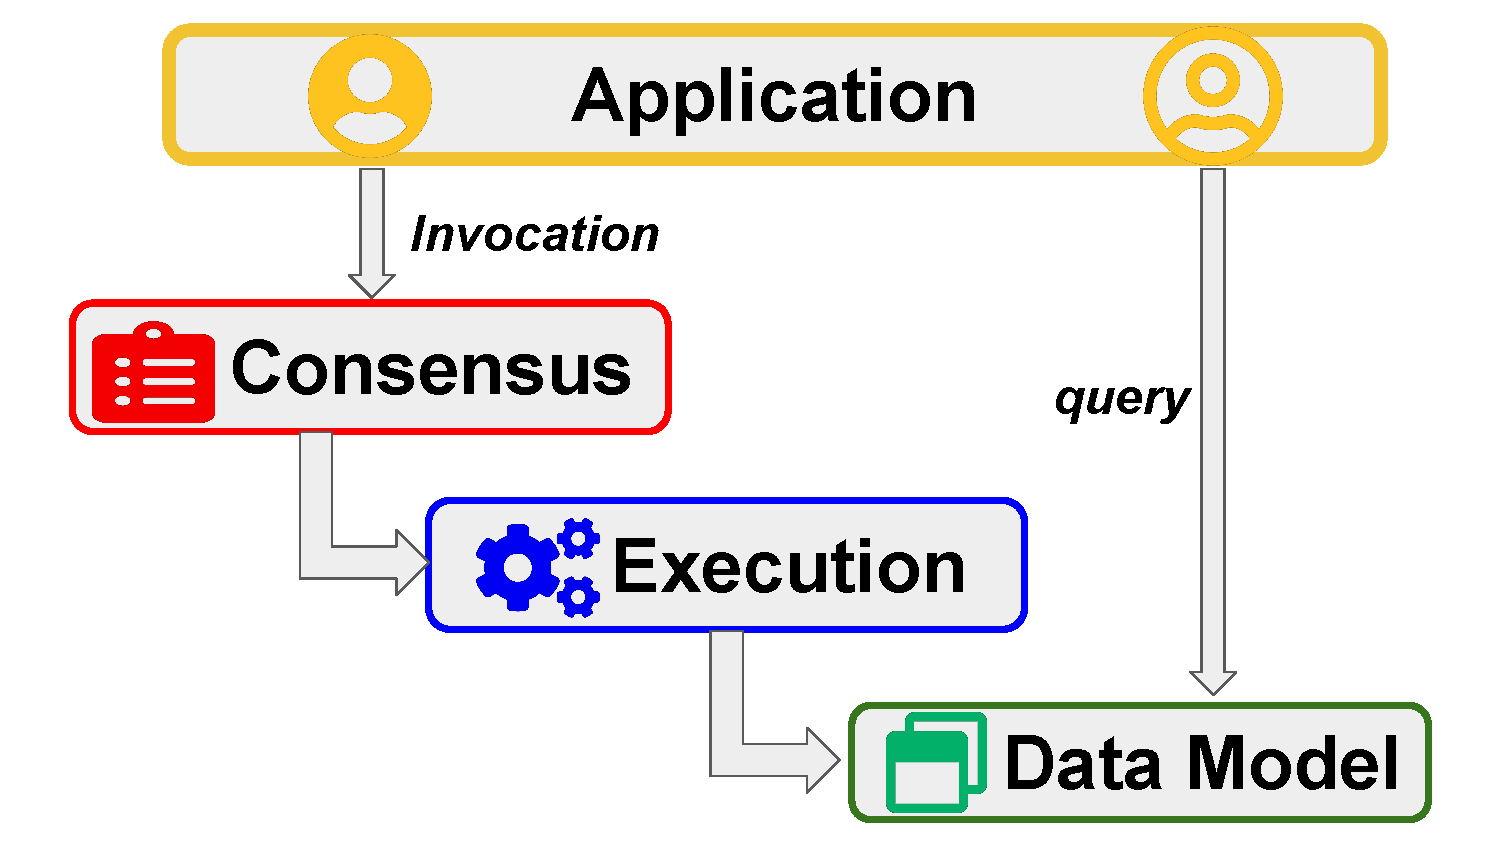
\includegraphics[width=0.8\linewidth]{diagram/intro/architecture.pdf}
  \vspace{\BeforeCaptionVSpace}
  \caption{Blockchain high-level architecture. }
  \subcaption*{State-mutating transactions must undergo the consensus and the execution components before persisting their effects at the data model layer, whereas ledger and state queries are directly answered by the storage component. }
  \label{diagram:intro:arch}
\end{figure}

\section{Vision, Motivation and Principle}

Our system-wide optimization primarily focuses on permissioned blockchains.
When compared with permissionless blockchains, permissioned blockchains resembles more to distributed databases and hence are more applicable to the database techniques.  
Their similarities and implication are summarized as follows: 

\textbf{Generic Workload Support. } 
Smart contracts of permissioned blockchains support arbitrary data transformation, like stored procedures in databases. And both of their invocation result into a transaction in their respective context. 
This is in contrast with permissionless blockchains, which mostly restrict their attention to the ownership transfer. 
Inevitably, permissioned blockchains raises for more challenges due to their generality.
Our optimization can no longer exploit the strong notion of asset ownership like in permissionless blockchains. 

\textbf{Authenticated Identity. } 
Analogous to distributed databases, permissioned blockchains operate under the authenticated setup.
Hence both categories of systems allow for more efficient state-machine replication consensus to withstand the byzantine failure. 
In comparison to permissionless blockchains, their PoW-like consensus (which is a must to mitigate Sybil Attacks) dominates the entire system performance. 
From this angle, the enhancement on other components of permissioned blockchains is necessary and worthwhile, as to side with their faster state-machine replication approach. 
Furthermore, the known membership relieves us from the identity problem. 
So that we will never get plagued by any Denial-of-the-service Attacks or Sybil Attacks throughout. 

The above commonalities explain why a number of entrepreneurs are actively exploring permissioned blockchains to replace their enterprise-ready databases. 
They seek to harness their common data processing capability while enjoying the additional decentralization and security that permissioned blockchains uniquely provide. 
However, their attempts are primarily hindered by the following limitations of the permissioned blockchains:

\textbf{Utility. }
Even though smart contracts open up opportunities for arbitrary transaction logic for blockchains, their provided utility is far from comparable to that of databases. 
For example, mainstream blockchains only provide procedural languages to encode the data transformation, such as Ethereum with Solidity and Hyperledger Fabric with Golang. 
But current relational databases already adopt the more expressive declarative SQL language, not to mention the enriched query features that databases develop over decades. 
In the face of growing demand, permissioned blockchains call for more data processing functionalities, like databases. 

\textbf{Performance. }
Another challenge is the low processing volume of permissioned blockchain to accommodate the business load. 
Researchers in BLOCKBENCH evaluated three blockchains with database workloads on the same testbed. 
Their results show that blockchains lag far behind databases in around two magnitudes. 
We believe the extra security properties of blockchains shall not solely account for such a huge performance gap. 
There must exist abundant optimization room available for the speedup. 

In the above, we lay out the optimization vision by showing vast similarities between permissioned blockchain and distributed databases. 
And we have also motivated such necessity by pinpointing the pain points for the adoption of blockchains in the industry. 
We now explain the three principles that our enhancement follows:

\begin{itemize}
  \item We break no security properties. We believe security lies at the core of blockchains. Although relaxing security assumptions is a standard engineering approach for the performance speedup, we do not find it scientific. A typical approach is to improve the system throughput by simply switching from byzantine tolerant consensus to crash failure tolerant. In our thesis, this principle can be manifested in the following two ways. Firstly, for the utility enhancement, we must preserve security on the added features. For instance, in Chapter~\ref{ch:prov}, we take special care to extend the tamper-evidence guarantee to the data provenance. On the other hand, any proposed procedures must be accompanied by their security analysis. This is why we dedicate \Cref{sec:txn:securityanalysis} on the security implication of the transaction reordering. 
  \item We adopt the modularized approach. We decouple a complex system into individual layers for the separate optimization. Modularization allows for the separation of concerns for the ease of reasoning. It also facilitates interoperability with independent optimization. 
  We follow the proposed architecture in BLOCKBENCH for our blockchain optimization in Chapter~\ref{ch:prov} and ~\ref{ch:txn}. In particular, we pinpoint our instrumentation with respect to each of four layers, as classified in Figure~\ref{diagram:intro:arch}. 
  \item Rather than building from the scratch, we ground our optimizations on Hyperledger Fabric v2.2, the most popular permissioned blockchain. Building on an existing system not only reuses its well-examined components, but this action by itself proves our practicality. Moreover, the results from a full-fledged system, instead of a prototype, are more convincing. And the evaluation is more meaningful when directly comparing with the vanilla baseline. 
\end{itemize}

\section{Optimization Basis}
\label{sec:intro:basis}
We incrementally apply our optimization on Hyperledger Fabric 2.2.0 into {\fs} and open source it~\cite{fsharp}. We fork its codebase with the commit hash \textit{2821cf}, the last commit on the branch \textit{release-2.2} when we start preparing this thesis. In later paragraphs, Fabric, without any version specification, all refers to this codebase snapshot. 

We now evaluate its throughput under out testbed and setup, which serves as the baseline. 
The testbed consists of a local cluster of 96 nodes. Each node is equipped with E5-1650 3.5GHz CPU, 32GB RAM, and 2TB hard disk. The nodes are interconnected via 1Gbps Ethernet. 
We dedicate five nodes to run \textit{peer} processes and three nodes for \textit{orderer} processes. 
(The distinction of \textit{peer} and \textit{orderer} processes can be found at~\Cref{sec:literature:execution:execute-order-validate}.  )
We configure Raft as the consensus protocol and all inter-node communication are protected by TLS encryption. 
Unless otherwise mentioned, all our following experiments in this thesis are conducted in the identical setup and the same testbed as this experiment.

We now present the primary results, after averaging over 3 times, in Figure~\ref{chart:intro:basic}. 
The first experiment is adapted from YCSB~\cite{cooper2010benchmarking}. 
Its workload consists of uniform write-only transactions, each inserting 1KB record. 
From Figure~\ref{chart:intro:basic:ycsb}, Fabric attains its peak throughput at around 1500 tps when the number of transactions per block is 1000 and beyond. 
In the second experiment, we evaluate Fabric against the Smallbank workload with 100K records, which follows a Zipfian distribution with $\theta=1$. 
We also vary the block size but control the requests at a rate which just saturates the system. 
We derive the saturated request rates from the previous YCSB experiment. 
For example, when a block contains 100 transactions, the request rate is 300 tps.
One can observe in Figure~\ref{chart:intro:basic:smallbank_blk} that the peak effective throughout reaches its peak at 600 transactions per block and 1200 tps request rate, instead of 1000 transactions per block in the previous experiment. 
It is because the block size introduces two interplay factors. 
On the one hand, a small block limits the system capacity.
As shown in Figure~\ref{chart:intro:basic:smallbank_blk}, the raw throughput, which includes the aborted transactions, grows with the block size. 
On the other hand, a large block implies that more transactions are concurrent. 
As explained in Chapter~\ref{sec:txn:theory}, concurrency exaggerates the conflicts, which leaves more transactions aborted and reduces the effective throughput. 
This aligns with our observation that the abort rate also increases with the block size.
The third experiment fixes the optimal setup for Smallbank, which is 600 transactions per block and 1200 tps request rate. 
We vary the Zipfian coefficient $\theta$ to control the skewness and present the effective throughout in Figure~\ref{chart:intro:basic:smallbank_skew}. 
One can observe that the Fabric's performance is susceptible to the request skewness, i.e., the greater $\theta$ leads to the lower throughput. 
In particular, as illustrated by the blue bar, it only attains 331 tps for the effective throughput when $\theta=1.5$, around 43.7\% of the peak. 
This set of experiments demonstrates the limited performance of Fabric and again calls for the speedup of permissioned blockchains. 

\begin{figure}[tp]
	\centering
    \begin{subfigure}{0.30\textwidth}
      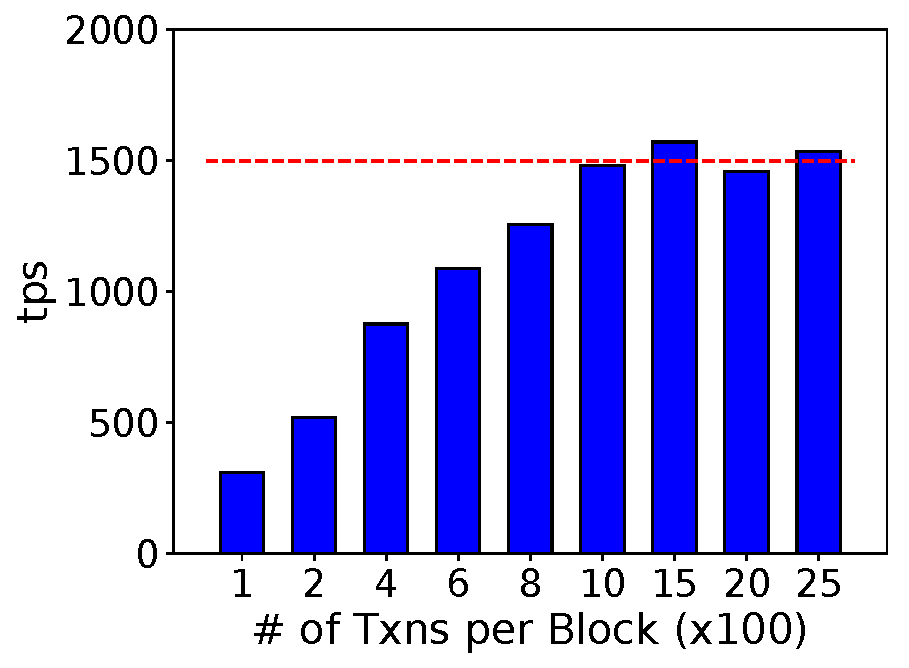
\includegraphics[width=0.99\textwidth]{chart/intro/ycsb.pdf}
      \caption{YCSB}
      \label{chart:intro:basic:ycsb}
    \end{subfigure}
    \begin{subfigure}{0.30\textwidth}
      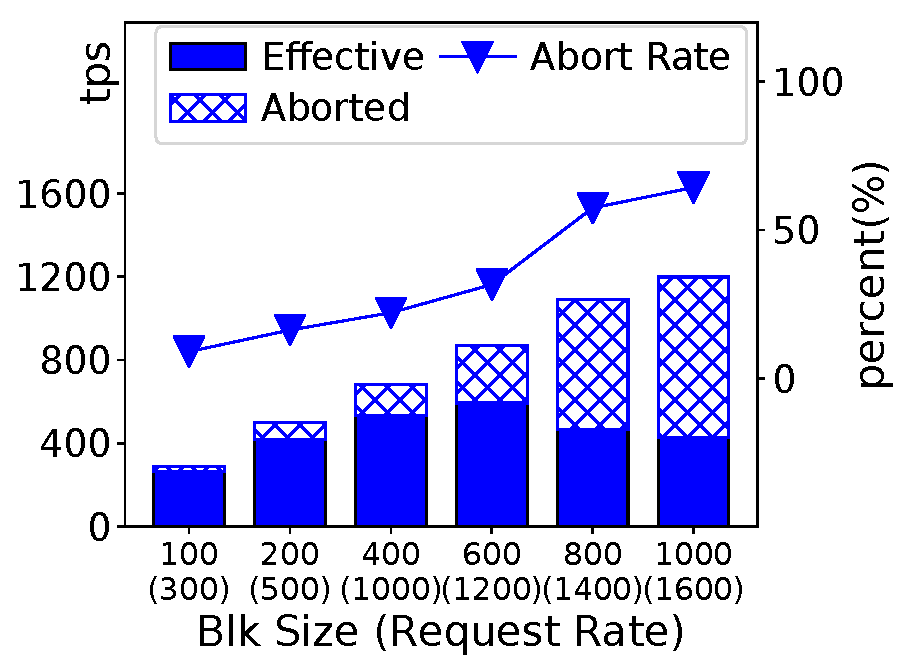
\includegraphics[width=0.99\textwidth]{chart/intro/smallbank_blk.pdf}
      \caption{Smallbank ($\theta=1$)}
      \label{chart:intro:basic:smallbank_blk}
    \end{subfigure}
    \begin{subfigure}{0.30\textwidth}
      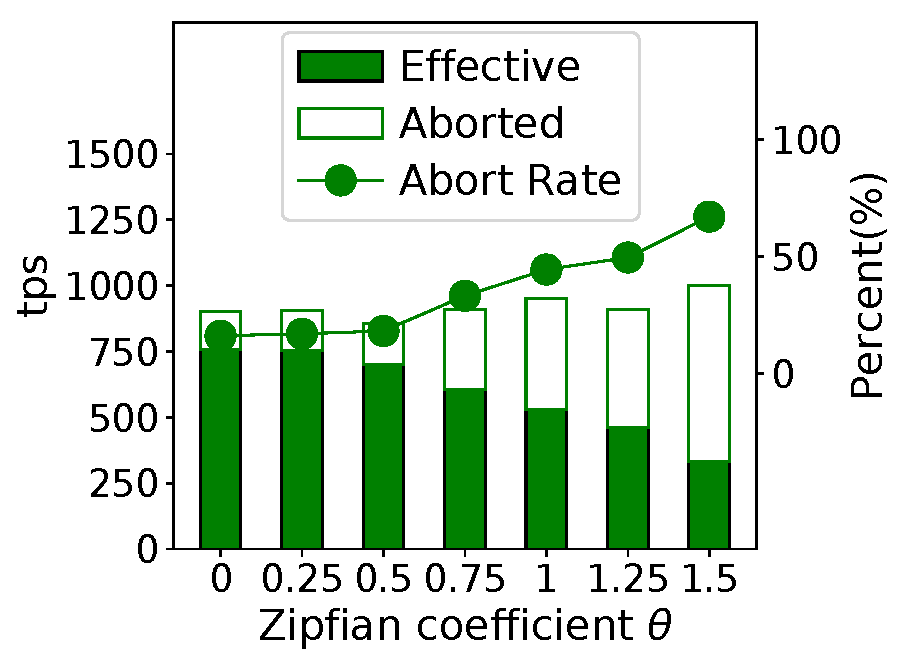
\includegraphics[width=0.99\textwidth]{chart/intro/smallbank_skew.pdf}
      \caption{Smallbank (skewed)}
      \label{chart:intro:basic:smallbank_skew}
    \end{subfigure}
    \caption{Primary evaluation results for Fabric }
    \subcaption*{(a) Fabric attains around 1500 tps at 1000 transactions per block, reaching its peak under the contention-free workload.(b) When Smallbank workload follows Zipfian distribution with $\theta=1$, Fabric reaches its peak (around 600 tps) at 600 transactions per block and 1200 tps request rate. (c) The skewness of the workload impacts on the Fabric's behavior. }
    \label{chart:intro:basic}
\end{figure}

\section{Thesis Synopsis}
We structure the rest of this thesis as follows. Chapter~\ref{ch:literature} overviews the recent year progress on both permissioned and permissionless blockchains. The covered literature spans from the database, distributed computing, and security communities. For the modularized fashion, we organize their reviews according to the classified layers in Figure~\ref{diagram:intro:arch}. This chapter ends with our critical analysis in this area. 

Chapter~\ref{ch:twin} proposes a taxonomy that unifies blockchains and distributed databases. 
The study considers both systems as the same type of distributed transactional systems, for the joint analysis on their respective focus. 
According to each dimension in the taxonomy, we devise corresponding workloads for the evaluation. 
Our results reveal the implication of their design choices. 
This comprehensive study sheds light on the optimization opportunities on permissioned blockchain with database techniques. 

Chapter~\ref{ch:prov} demonstrates our optimization for the utility. 
We first explain the added business value when data provenance is exposed to smart contracts. 
Then we introduce how lineage information in blockchains are captured, stored, and queried. 
The greatest contribution of our proposal is to extend the integrity property for the entire data evolution history. 
After implementing it into {\fs}~(or Fabric\# for short), the empirical evaluation demonstrates the negligible performance and storage overhead with this additional feature. 

Chapter~\ref{ch:txn} demonstrates another optimization on the performance. 
The work originates from our following subtle observation:
the execute-order-validate architecture in permissioned blockchains may over-abort transactions under the Serializable isolation level. 
Borrowed from the well-established transactional analysis from databases, we reason about the potential of transaction reordering to streamline the execution schedule. Based on the developed insight, then we adapt {\fs} to attain the theoretical limits. 
And the improvement is empirically demonstrated with our remarkable speedup, compared with the vanilla Fabric and the other state-of-the-art. 

At last, we wrap up the thesis with the conclusion and future directions in Chapter~\ref{ch:conclu}. 
In light of a variety of Fabric variants referenced and benchmarked in this thesis, we compile all for the clarity in Appendix~\ref{sec:append:variants}. 


% \SetPicSubDir{ch-Rice}
% \SetExpSubDir{ch-Rice}

\chapter{Literature Review}
\label{ch:literature}
In this chapter, we lay out the foundation of blockchains and explore a systematic exposition on their recent progress.
We organize the review based on the abstract layers as classified in Figure~\ref{diagram:intro:arch}, before identifying the research gap. 

\section{Data Model Layer}
\label{sec:literature:datamodel}
The data model in blochchains concerns on how to organize data that reflect the latest states, and model the ledger that records the historical transactions. 

\subsection{State Organization}
There are two state organizations in blockchains, the unspent transaction output-based (UTXO) and the account-based. Their key difference lies whether systems explicitly maintain the states. We illustrate both schemes in Figure~\ref{diagram:literature:data_model}.

\begin{figure}
    \centering
    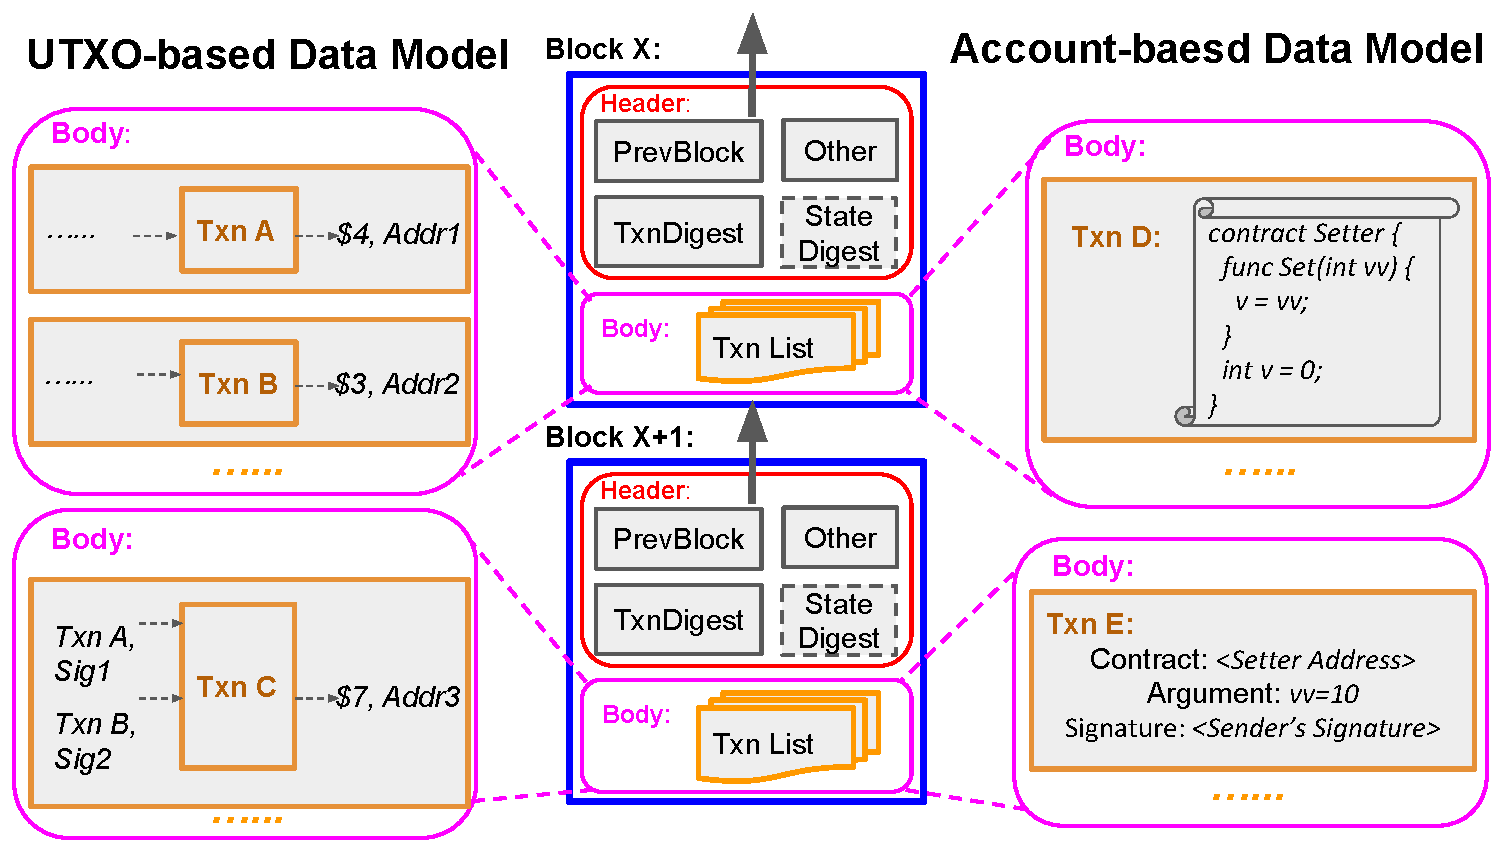
\includegraphics[width=0.8\linewidth]{diagram/literature/data_model.pdf}
    \vspace{\BeforeCaptionVSpace}
    \caption{The Unspent Transaction Output (UTXO) model vs the Account-based model. }
    \label{diagram:literature:data_model}
\end{figure}

\textbf{UTXO Model.}
UTXO operates on the transaction basis. In their structure, a transaction consists of multiple inputs and outputs. Each output is associated with an amount of cryptocurrency and an cryptographic puzzle. Any future transaction can reclaim this amount in its input, by providing the puzzle answer and referencing the previously unspent output. An canonical puzzle and its solution can be an address in the format of a public key hash, and a digital signature from the corresponding private key. Notably, the UTXO model does not bookkeep the balance to addresses. All transactions in the ledger form a Direct Acyclic Graph that records the cryptocurrency flow, where identity hides under the anonymous addresses. 

Bitcoins, due to its decentralization and anonymity, provide a terrain for financial crimes, such as drug dealing and the money laundry. There are a number of attempts to exploit the transactional graph, and identify the pattern for the detection~\cite{fleder2015bitcoin,ron2013quantitative,weber2019anti}. 
Some analysis relies on the graph linkage to discover the identity~\cite{ober2013structure,gaihre2018bitcoin,moser2013anonymity} or other information to predict the bitcoin price~\cite{greaves2015using}. 

\textbf{Account-based Model.}
Due to its simplicity, the UTXO model is solely applicable to cryptocurrency-based platforms. 
To support more general workloads, Ethereum introduces the smart contract to encode Turing-complete logic. 
In their design, a transaction either takes in the form of a contract deployment with the executable code. 
Or a transaction provides the execution context to invoke a contract. 
In all cases, each transaction is tagged with the digital signature of the sender. 
In addition, each blockchain peer must explicitly compute for contract states, including the cryptocurrency balance, in each account. 
Such requirement is enforced by the blockchain protocol that all peers shall reach consensus on a post-execution state digest in the block header. 
In contrast, the UTXO-based blockchain only requires a digest for the transaction integrity.

The account-based data model with smart contracts transition a blockchain into a more general processing platform. 
But it inevitably incurs more vulnerability from the additional complexity. 
For example, some malicious users might run an infinite loop in a transaction to waste system resources. 
To defer such Denial-of-service Attack in the permissionless setting, all blockchains are designed with an incentive-compatible mechanism to prevent the abusive usage. 
For example, Ethereum charges transaction senders with the transaction fee, in an amount proportional to the number and the complexity of contract operations~\cite{wood2014ethereum}.
Recently, a number of research works show that how to quantify such complexity and charge accordingly is not that intuitive than previously thought~\cite{chen2017adaptive,web:txn_spam}. 
Despite this, computational-heavy transactions may still render blockchains securely-flawed: some researchers reveal that rational block validators tend to skip their execution to gain an edge for the next block mining~\cite{luu2015demystifying}.
It is because all the transaction fee is credited to the block miner. 

\subsection{Ledger Abstraction}
The term \textit{blockchain} originates from the fact that the ledger takes in the form of a hash chain of blocks. 
Initially, the rationale for Bitcoin to batch transactions into blocks is to amortize the cryptographic overhead.
However, this single-chain structure prohibits the concurrency, as all participants must sync up on the unique ledger tip. 
To address this problem, numerous studies have transformed a chain into a direct-acyclic graph (DAG), and then derive a total order of transactions~\cite{sompolinsky2015secure,kiayias2017trees,li2018scaling,srivastava2018phantom}. 
The exact ledger format is strongly tied to their consensus. 

Meanwhile, batching trades off the latency for the throughput, as PoW bounds the block interval by the network delay. 
But from the perspective of permissioned blockchains. such tradeoff is not worthwhile: the state-machine replication consensus places no such restriction on the block interval. 
This observation accounts for why some researchers abandon the canonical block-based design but directly work upon transactions~\cite{istvan2018streamchain}. 
For a similar reason, we have observed a number of proposals known for their transaction-based DAG-typed ledger~\cite{lemahieu2018nano,churyumov2016byteball,divya2018iota}. 

\section{Execution Layer}
The execution layer concerns on how to process transactions. 
Different blockchain platforms adopt their distinct execution platforms, such as the Docker environment for Hyperledger Fabric and Ethereum Virtual Machine (EVM) for Quorum. 
Despite their implementation differences, the execution architecture of any blockchains falls into either of the following categories. Figure~\ref{diagram:literature:execution} presents their distinction. 

\begin{figure}
    \centering
    \begin{subfigure}{0.8\textwidth}
      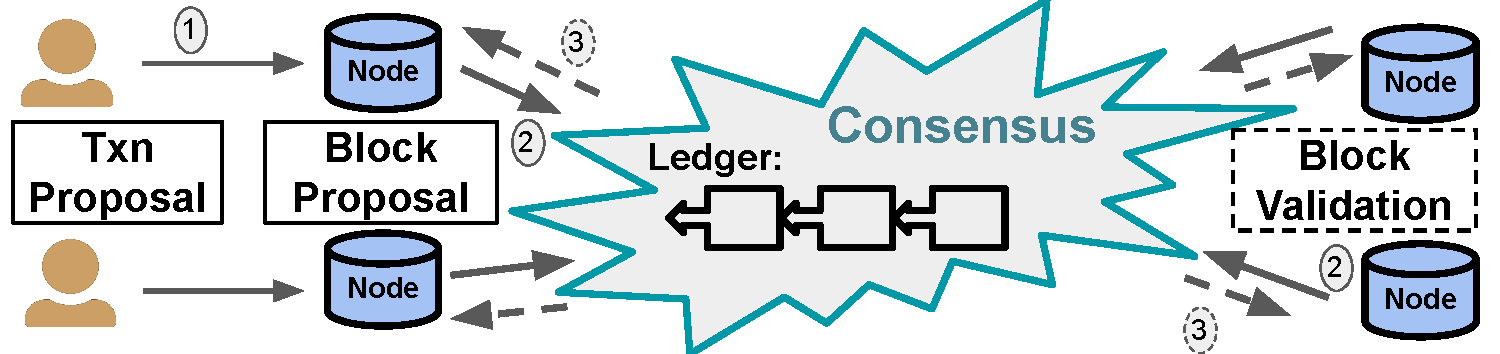
\includegraphics[width=0.99\textwidth]{diagram/literature/ox_arch.pdf}
    \end{subfigure}
    \begin{subfigure}{0.8\textwidth}
      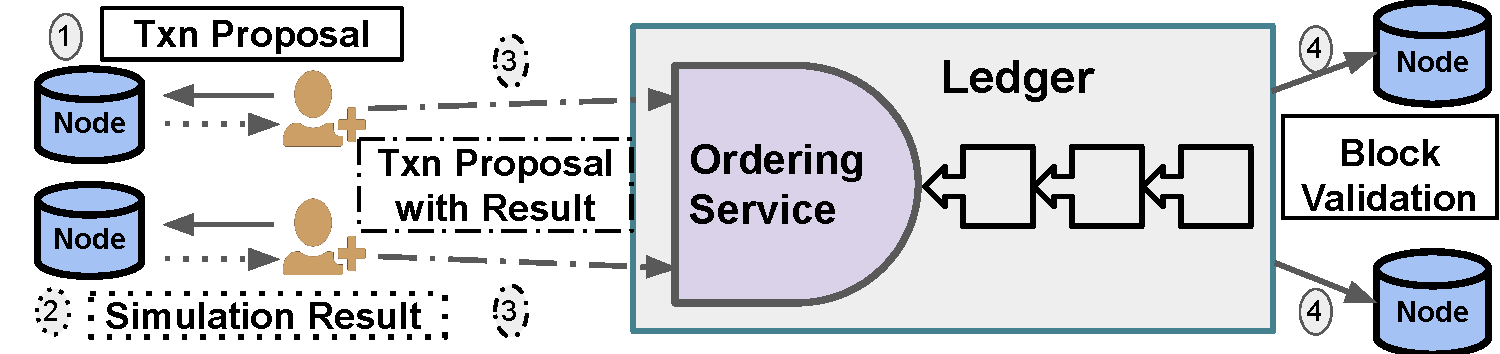
\includegraphics[width=0.99\textwidth]{diagram/literature/eov_arch.pdf}
    \end{subfigure}
    \caption{The Order-execute vs. Execute-order-validate architecture. }
    \label{diagram:literature:execution}
\end{figure}

\subsection{Order-execute Architecture}
\label{sec:literature:execution:order-execute}
In the Order-execute architecture, each peer serially executes transactions, based on the established order according to the ledger by the consensus. 
Bitcoin as well as all cryptocurrency-based blockchain adopts this concurrency-free design, simply because the consensus, rather than the execution layer, decides on the system performance. 
Moreover, sequentiality makes it easy to reason about the system behavior. 

Despite this, things still get convoluted when transactions deal with Turing-complete logic. For example, many security researchers have demonstrated that Solidity contracts in Ethereum are far more tricky than expected~\cite{luu2016making,parizi2018smart,atzei2017survey}. 
Due to some subtle misunderstanding on operation semantics on EVM, flawed contracts can be exploited by adversaries to gain profits. 
And the problem is further exaggerated given the transparency and the irreversibility of blockchains. 
The DAO hack shows that such an attack is not only a possibility in the theory but a true threat in reality~\cite{santos2018dao}.
In the meantime, there come along a series of empirical guidelines and practical tools to aid the contract development~\cite{ducasse2019open,jeng2019step,bai2018formal,tikhomirov2018smartcheck}. 

Through the Order-execute architecture takes on the sequential approach, it is never insulated from the concurrency topic. 
For example, after remarking the reminiscence between contract bugs in blockchains and data races in shared-memory programming, researchers propose a novel viewpoint on the security issues of contracts, from the concurrency perspective in distributed computing~\cite{herlihy2019blockchains,sergey2017concurrent}. 
In ~\cite{dickerson2019adding}, researchers explore to tentatively execute transactions in parallel and then fall into serial if encountering a conflict.  
Instead of speeding up the entire system, the goal of the concurrency is to facilitate the block validation, so that validators can gain a competitive edge on the next block mining. 
Quantitative analysis of the transaction graph shows abundant concurrent chances in mainstream blockchains~\cite{reijsbergen2020exploiting,saraph2019empirical}. 

\subsection{Execute-order-validate Architecture}
\label{sec:literature:execution:execute-order-validate}
Execute-order-validate architecture is proposed in Hyperledger Fabric v1.0~\cite{androulaki2018hyperledger}. 
Rather than taking a monolithic approach, the system is designed with two types of blockchain nodes: peers which execute smart contracts and validate blocks, and orderers which order transactions. 
A transaction pipeline is divided into three phases. 
In the Execute phase, a client requests a subset of peers to execute the transaction speculatively. 
The client collects the results and signatures from peers and sends them to the orderers. 
In the Order phase, orderers order the transactions and batch them into blocks.
For modularity, orderers do not inspect the transaction details. 
In the Validate phase, each peer pulls blocks from the orderers and independently validates each block before persisting the results. 
The block validation process firstly verifies whether transactions satisfy the endorsement policy, i.e., enough number of peers show the endorsement by their signature. 
Then validation procedure checks for conflicts in the read/write sets for each transaction. 
The invalid transactions will not persist their effects, even though they are part of the ledger. 
Read-only queries only involve the Execute phase. 

This architecture brings additional benefits compared to Order-execute architecture. 
Firstly, the endorsement policy decouples the trust condition of a contract from the consensus. 
For example, a transaction with the endorsement on execution results from only one of three peers can be considered valid. 
In contrast, the Order-execute architecture mandates the majority of peers to agree on the contract result. 
Secondly, it preserves confidentiality by restricting the execution to specify peers.
Clients, by knowing results before transactions are effected, can also minimize the uncertainty. 
Lastly, speculative execution at the start fits well for the concurrency.
It greatly facilitates computation-heavy transactions, which would queue up in the sequential Order-execute architecture. 

However, such concurrency comes with the cost, which manifests as the aborted transactions for the serializability. 
We have empirically demonstrated that in Figure~\ref{chart:intro:basic} and will elaborate this issue in Chapter~\ref{ch:txn}. 
In light of this, Fabric++ reorders transactions during the Order phase to minimize the abort~\cite{sharma2019blurring}. 
OXII architecture is featured for an additional dependency resolution phase at the start~\cite{amiri2019parblockchain}.
So that it enables for a concurrency-friendly transaction schedule. 
OXII relies on the core assumption that the dependency can be extracted by inspecting the contract codebase. 
In the same spirit, XOX architecture runs a patch-up code to streamline a contended transaction~\cite{gorenflo2020xox}. 
The dependency captured during the transaction execution determines this snippet of code. 

\section{Consensus Layer}
Byzantine-tolerant consensus differentiates blockchains from other distributed systems. 
Proof-of-work (PoW), initially proposed in Bitcoin, opens up a new horizon on incentive-based protocols. 
Meanwhile, permissioned blockchains revitalize the interest of 
state machine replication approach to address the arbitrary failure. 

\subsection{PoW and its Analysis}
The essence of PoW is a hard-to-solve and easy-to-verify puzzle. 
The protocol prescribes that the first solver has the privilege to broadcast a new block on the tip of the ledger. 
By adjusting the puzzle difficulty such that the solving duration exceeds the maximum network delay,
all blockchain participants can then sync up on the unique chain. 
In Bitcoin, the puzzle solution is a nonce to make the block hash value prefixed with enough zeros. 
The block proposer gets compensated for the hashing power with the newly-minted cryptocurrencies and the transaction fee. 

In the context of Bitcoin, the solution-finding process is called \textit{mining}. 
Due to the irreversibility of the hash function, mining is fair to all participants, including the adversaries. 
Ruling out the possibility that adversaries control the majority of the hash power, it results into the following two implications.
If the adversaries pour all their resources to mine on a shorter chain fork, 
that fork is impossible to catch up the longest chain, where the rest of honest power concentrates. 
Nakamoto has bounded this possibility to be exponentially small in the original whitepaper~\cite{nakamoto2019bitcoin}.
More in-depth mathematical frameworks have been established to reason about the mining behavior ~\cite{gervais2016security,kiayias2015speed,ren2019analysis,miller2014anonymous,garay2015bitcoin}. 
On the other hand, honest block proposers, aware that the longest chain is hardly revertible, are incentivized to extend on it. 
It is because their proposed block contains a coinbase transaction that credits the minted cryptocurrencies to proposers. 
Only the block is in the longest chain then this transaction can take into effect. 

Inevitably, the longest-chain-rule may lead to two divergent forks during the asynchronous network period. 
When the network delay exceeds the block interval, two honest participants may generate two different blocks but on the same height. 
The longest-chain-rule will eventually resolve to a unique chain when the network partition heals.
Hence, transactions in the ledger may not be secure given that they might reside on a shorter, to-be-pruned fork. 
Considering this, clients are advised to wait for their transactions until deep enough, before considering them committed. 
Intuitively, this depth, quantified by the number of blocks behind, balances between latency and security. 
In the meantime, the block interval and the block size controls the tradeoff between throughput and security. 
The shorter interval and the larger block imply greater system capacity. 
But it compromises the security, i.e., the network may not propagate a block to each participant before the next block is generated. 

Moreover, \cite{eyal2014majority} suggests that adversaries may not be incentivized to follow the default mining policy, i.e., mining on the longest chain and broadcast the block immediately. 
Instead, they may temporally withhold mined blocks and selectively publish them to gain extra profits.
Since then, more mining policies are discovered which allows adversaries to gain a competitive edge \cite{nayak2016stubborn,courtois2014subversive},
even infiltrating other mining pools to waste their resources~\cite{luu2015power,eyal2015miner}. 
Researchers employ a Markov Decision Process to find the optimal mining policy and explore the performance-security tradeoff~\cite{gervais2016security,sapirshtein2016optimal}.

\subsection{The Enhancements on PoW}
PoW has long been plagued for its energy assumption. 
In 2019, Bitcoin's electricity consumption is reported to reach 45.8 TWh. 
Naturally, several researchers propose to transform PoW to be more eco-friendly, 
or at least dedicate resources to useful tasks. 
We refer to these PoW-based enhancements as Proof-of-X (PoX). 

The major challenge of PoX is to replace the original computation-intensive puzzle and preserve its long-to-solve and easy-to-verify nature. 
For example, Proof-of-Stake (PoS) requires miners to stake a certain amount of cryptocurrencies~\cite{king2012ppcoin}. 
The stake will be confiscated if the proposed blocks are found to be invalid. 
One can find the adoption of PoS in the following blockchains~\cite{kiayias2017ouroboros,david2018ouroboros,bentov2016snow} and their security analysis in~\cite{nguyen2019proof,li2017securing,brown2019formal}. 
Proof-of-Elapsed-Time (PoET) replies on the Trusted Execution Environment to attest block validators that miners have waited enough time before the next block proposal~\cite{chen2017security}. 
To fully exploit the consumed resources to useful works, 
Proof-of-Retrievability is repurposed for the data archival~\cite{miller2014permacoin}, Proof-of-Prime-Number for the prime number searching~\cite{king2013primecoin}, and others for matrix product problems~\cite{shoker2017sustainable}. 

Another enhancement direction is to optimize the primitive PoW. 
Researchers adapt the puzzle-computation to resist ASIC-equipped mining and deter power centralization~\cite{zamanov2018asic,cho2018asic}. 
On the other hand, they refine the PoW mechanism to increase the system capacity.
For example, the original PoW groups the leader election and transaction proposal together. 
Bitcoin-NG decouples these two tasks, by allowing a puzzle solver to continuously propose transactions until the next solver emerges~\cite{eyal2016bitcoin}. 
GHOST incentives miners to extend on the heaviest sub-tree instead of the longest chain~\cite{sompolinsky2015secure}. 
This is to better recycle orphaned blocks. 
Conflux furthers replies on GHOST to determine the pivot chain and use the pivot chain to decide on a direct-acyclic graph, whose topological order determines the overall transaction sequence~\cite{li2018scaling}. 
The OHIE is renowned for its multiple-chain structure to harness the distributed network setup~\cite{yu2020ohie}. 
Its protocol drives each chain to grow at the same pace. 

\subsection{Byzantine Fault-tolerant Consensus}
The state-machine replication method to address byzantine consensus resurges with the popularity of blockchains. 
The Byzantine-fault tolerant consensus problem involves a number of nodes with initial different proposals. 
The problem requires honest nodes to reach agreement on one of the proposals, while reserving the safety (no possibility of disagreement) and liveness (guarantee of termination)~\cite{lamport2019byzantine}. 
And this must hold true under the premise that a fraction of malicious nodes may perform arbitrary action. 
Compared to Bitcoin, this problem modeling is more general, i.e., it is not targeting only on the ledger and no incentives can be hinged on. 

Long before Bitcoin, PBFT has provided the first-ever practical approach.
It achieves the consensus in $O(n^2)$ message complexity where $n$ is the number of nodes. 
Quorum adopts a PBFT-variant, IBFT as one of its consensus options but still requires for $O(n^2)$ messages~\cite{saltini2019correctness}. 
Tendermint reduces this bound to $O(n)$ but forgoes the network responsiveness~\cite{buchman2016tendermint}. 
In a word, unlike PBFT, the progress of Tendermint is dependent on the maximum network delay, rather than the actual message transmission delay~\cite{amoussou2019dissecting}. 
Hotstuff augments on the two-phase approach of PBFT and Tendermint into three phases of the message exchange~\cite{yin2019hotstuff}. 
But it achieves both network linearity ($O(n)$ message complexity) and the responsiveness. 

While the above series of researches are rooted from PBFT, researchers in VMWare address the problem from a new angle. 
They remark the possibility to reach consensus in a single phase, given more number of nodes have acknowledged the proposal than normal. 
Based on this insight, they start from Fast Byzantine Paxos~\cite{martin2006fast} and Zyzzyva~\cite{gueta2019sbft}, and lead into a series of re-analysis~\cite{abraham2017revisiting} and re-design~\cite{abraham2018revisiting, gueta2019sbft}. 
Their novelty comes from a fast path if more-than-normal acknowlegements have been collected before a timeout. 
Otherwise, the consensus falls backs to the standard two-phase pipeline.  

FLP Impossibility Result imposes no deterministic, safe and live protocols under the asynchronous network~\cite{fischer1985impossibility}. 
The above Byzantine-tolerant consensus protocols trade the liveness for the safety during the network partition. 
In other words, disagreement never occurs even the network loses the connection. 
Correspondingly, there also exist a number of approaches that rely on the network synchrony for the safety~\cite{abraham2020sync,abraham2017efficient}. 
In this manner, these protocols behave like PoW in Bitcoin, i.e., a chain will fork under the asynchronous period. 
In their design, the strict network assumption comes into play when to reliably broadcast the latest, majority-acknowledged block proposal. 
Notably, Flexible BFT mixes two types of deterministic protocols together, so that clients can draw their own commit decisions at their discretion on the network condition~\cite{malkhi2019flexible}. 

Randomness is another alternative route to break the Impossibilty, in order to reach agreement on the ledger. 
For example, HoneyBadgerBFT combines a variety of randomized agreement protocols~\cite{miller2016honey}. 
So that it achieves linear message complexity, as PoW in Bitcoin. 
As the carry-on work, BEAT provides a diversity of randomized protocols that tailors for various application demands~\cite{duan2018beat}. 
Such randomization takes in the form of the unpredictable network connectivity in~\cite{rocket2019scalable}.
In its design, each node repetitively queries for the proposals from the neighbors that it knows of. 
It then determines his own proposal from the majority of query results and uses it to respond for other's queries. 
Eventually, all honest nodes are probabilistically steered towards a uniform outcome, even though a limited fraction may cheat. 

\subsection{Committee-based Consensus}
Blockchains with the committee-based consensus select a single or multiple representative committees, which then establish the ledger with the above state-machine replication consensus. 
This idea has been dated back to PeerCensus~\cite{decker2016bitcoin}. 
But their application may not be that straightforward. 
It is because these off-the-shelf protocols require for strong assumptions, including identity management, member constitution, and so on. 
To cater for these conditions, most blockchains must couple wth some additional procedures, especially on the fair committee formation. 
For example, Algorand determines a single committee based on the Verifiable Random Function (VRF)~\cite{gilad2017algorand}. 
In particular, nodes must compute a value with VRF from its private key and a common seed. 
Only those with specific values are allowed to join the consensus with their public keys. 
VRF remains unpredictable without knowing the common seed beforehand. 
By starting from an unbiased random seed, Algorand guarantees that no adversaries may dominate a committee. 
Omniledger depends on the Randhound to achieve the decentralized and unbiased randomness, and power the multi-committee establishment~\cite{kokoris2018omniledger}. 
Byzcoin repurposes PoW to determine the membership for a single committee~\cite{kogias2016enhancing}. 
PoW not only guarantees the randomness but also resists the Sybil attacks under the permissionless setting. 
RapidChain also uses PoW to determine participants, from which it breaks into multiple committees with a theoretical-involved method~\cite{zamani2018rapidchain}. 
Elastico directly uses PoW nonce and group solvers with common prefixes into one of the committees~\cite{luu2016secure}. 
Such randomness for the committee formation comes from Trusted Execution Environment in AHL~\cite{dang2019towards}.
Not that all the above systems are subject to the periodic committee re-configuration between epochs. 
This prevents adaptive adversaries to exploit the setup and infiltrate honest nodes. 
The reconfiguration can be a full swap like in Elastico~\cite{luu2016secure}, Algorand~\cite{gilad2017algorand}, and Omniledger~\cite{kokoris2018omniledger}, or in a rotational manner like Byzcoin~\cite{kogias2016enhancing}, RapidChain~\cite{zamani2018rapidchain}, and AHL~\cite{dang2019towards}. 

We also observe several blockchains adopt a non-technical solution on membership management. 
For instance, a central authority decides on the validators' role in RSCoin~\cite{danezis2015centrally}. 
The participants and their weight in Libra~\cite{baudet2019state} and EoS~\cite{xu2018eos} are pre-determined according to their initial investment. 
Chainspace completely sidesteps the committee formation problem~\cite{al2017chainspace}. 
It leaves the behavior of malicious committee audible under the premise that they can be enforced by an external entity.

\section{Application Layer}
Blockchains provide unique decentralization, auditability, transparency, and irreversibility, adding abundant value to real-world applications. 
The most natural use case is to rely on the decentralized ledger as a trustworthy chronological logbook. 
For example, the Bitcoin protocol allows for a 40 byte of arbitrary data piggybacked at \textit{OP\_RETURN} opcode~\cite{opreturn}.
Several applications exploit this payload to use as a message commitment. 
So that one in the future can verify its existence, the creation time and the source of the origin. 
More advanced usage can be found in~\cite{maesa2017blockchain}, where this payload is used to encode the right transfer of the external resource access, and in~\cite{wu2017voting} for the e-voting. 
This survey investigates a broader range of applications and quantifies their the overhead of the piggybacking scheme~\cite{bartoletti2017analysis}. 

Another popular application is the token management.
Unlike the built-in cryptocurrency, the token is associated with external assets. 
The assets may range from vouchers, IOU, copyrights, and tangible objects. 
So that one may redeem the asset in the real world, by showing the cryptographic proof of the token possession in the blockchain. 
For example, one may get a one-for-one exchange between Tether tokens and US dollars. 
We observe most of these applications operate on Ethereum, especially to hinge on the official provided ERC20 token standard~\cite{wiki:ERC20}.
In particular, ERC20 is a smart contract that defines a common list of rules on token operations.  
Any token issuer can deploy its own version of the ERC20 contract with the prevision of the initial ownership and the total of the supply amount. 
The transfer of tokens takes in the form of the contract invocations. 
So that their transactions are secured by Ethereum.
ERC20 token is getting widespread with a growing number of Initial Coin Offering (ICO). 
This study reveals that there are more than 64k distinct ERC20 tokens~\cite{victor2019measuring}.
We refer readers to~\cite{victor2019measuring,somin2018network,chen2020traveling} for the analysis of their transaction pattern. 

To further unleash the blockchain potential, plenty of business proposals explore its intermediary-free data processing capabilities to the banking industry~\cite{guo2016blockchain}, the supply chain management~\cite{tse2017blockchain,saberi2019blockchain,korpela2017digital}, Internet-of-Things(IoT)~\cite{novo2018blockchain,huh2017managing,khan2018iot}, the autonomous governance~\cite{diallo2018egov,atzori2015blockchain}, identity service~\cite{lim2018blockchain,lootsma2017fintech}, medical record ownership control~\cite{azaria2016medrec,medilot}, collaborative shared databases~\cite{peng2020falcondb,el2019blockchaindb} and so on. 
In all the above cases, blockchains provide a unique trust-building platform that enforces the business process.
These processes usually involve multiple stakeholders with the conflict of interest.
Along with the popularity, some researchers voice out their concern about the improper blockchain usage. 
\cite{wust2018you} criticizes this worrying trend by critically analyzing several unreasonable cases. 
\cite{yaga2019blockchain,chowdhury2018blockchain,wust2018you} provide empirical guidelines for applications to choose between blockchains and conventional databases. 
In their opinion, the absence of the central authority is the deciding factor for the blockchain adoption. 
This absence may be due to the entangled interest in the application, the trust deficit from the hostile environment or etc. 
Otherwise, the expense of dis-intermediation, in terms of the extra storage and performance, far outweighs other blockchain-provided features. 
Most similar business requirements, such as the provenance support and state integrity, can be more efficiently satisfied with other technical solutions.
For example, QLDB, as a centrally administrated, in-cloud database, provides a verifiable storage~\cite{qldb}. 
In other words, the QLDB vendor is technically possible to tamper the data or refuse to deliver the service, despite the fact that all this action will leave evidence. 
Blockchains, however, is capable to prevent such arbitrary behavior due to their decentralized consensus. 
But it is questionable whether such additional security guarantee is worthwhile for most applications. 

\section{Benchmarks and Surveys}
Even though the aforementioned references cover most representative research works, they are far from comprehensive to draw an overall picture on the recent blochchain progress. 
For a wider range of exposition, we compile blockchain-related surveys with their focused layers in Table~\ref{tab:literature:survey}. We also tabulate reported benchmarks with their selected systems in the table.

\begin{table}[]
  \caption{Blockchain-related surveys and benchmarks}
  \label{tab:literature:survey}
  \centering

  \begin{tabular}{l|l|l}
    \hline
                             & \textbf{Layer} & \textbf{Focus}                                                                                       \\ \cline{2-3} 
    \multirow{4}{*}{\textbf{Surveys}} & Execution      & Ethereum Contract Security~\cite{li2020survey,atzei2017survey,chen2020survey,praitheeshan2019security}                                                                           \\ \cline{2-3} 
                             & Consensus     &  \cite{wang2019survey,nguyen2018survey,xiao2020survey,garay2020sok,consensus_survey}                                                                                                 \\ \cline{2-3} 
                             & Application    & \begin{tabular}[c]{@{}l@{}}Internet-of-Things~\cite{novo2018blockchain,wu2019comprehensive,wang2019iotsurvey} \\ Banking~\cite{guo2016blockchain,cocco2017banking,peters2016understanding} \\ Others~\cite{mollah2020blockchain,al2019blockchain,blossey2019blockchain,zhuang2020blockchain}\end{tabular}                                  \\ \cline{2-3} 
                             & Others         & \begin{tabular}[c]{@{}l@{}}Technical Overview~\cite{zheng2018blockchain,lin2017survey,dinh2018untangling}\\ Chain Interoperability and Sharding~\cite{zamyatin2019sok,wang2019sok,yu2020survey}\\ Data Privacy~\cite{feng2019survey,joshi2018survey,mohanta2019blockchain} \end{tabular} \\ \hline
    \multicolumn{2}{l|}{\textbf{Benchmarks}}           & \begin{tabular}[c]{@{}l@{}}Hyperledger Fabric~\cite{dinh2017blockbench,thakkar2018performance,nasir2018performance,ruan2019blockchains,pongnumkul2017performance,tinguely2019benchmarking}\\ Ethereum\cite{dinh2017blockbench,pongnumkul2017performance,rouhani2017performance,chen2018comparative} \\ Quorum~\cite{ruan2019blockchains,baliga2018performance} \\ Parity~\cite{dinh2017blockbench} \\ Corda~\cite{cordaperf,tinguely2019benchmarking} \end{tabular}                                  \\ \hline
    \end{tabular}
\end{table}

\section{Lessons learnt from the Review} 
Our above review reveals a mismatch between the focus of the industry and academia on blockchains. 
In particular, researchers place great emphasis on their security aspects. They restrict their attention on the incentive-based consensus, and UTXO-based cryptocurrency in permissionless blockchains. On the other hand, entrepreneurs in the industry show the most interest in the intermediary-free data processing capabilities from permissioned blockchains. 
In the meantime, we observe most researchers treat a blockchain as it is, but few of them realize its vast similarities to distributed databases. A few work with this awareness juxtapose permissioned blockchains and distributed databases for the joint study. 
But their analysis leaves much room for improvement: they either only show the blockchains' inferior performance to databases~\cite{dinh2017blockbench,chen2018comparative}. Or they compare their distinct value-addition properties for applications~\cite{chowdhury2018blockchain,wust2018you,yaga2019blockchain}. 
But they ignore a promising area, which is to optimize permissioned blockchains with database-specific techniques to support general workloads. 

Our thesis moves a step forward along this direction. 
We first classify blockchains and distributed databases under the same taxonomy.
Based on this framework, we jointly understand their design choices and behavior (Chapter \ref{ch:twin}). 
With the developed insights, we extend the provenance support to smart contracts to improve utility (Chapter \ref{ch:prov}). Then learning from databases, we explore reordering techniques to reduce the transaction abort. 
This performance enhancement applies to any blockchains with execute-order-validate execution pipeline (Chapter \ref{ch:txn}).  


\chapter{Twin Study}
\label{ch:twin}
\section{Introduction}
\label{sec:twin:intro}

The very first blockchain system, that is Bitcoin~\cite{nakamoto2019bitcoin}, is a decentralized ledger for
recording cryptocurrency's transactions. The ledger consists of multiple blocks chained together with cryptographic
hash pointers, each block containing multiple transactions. This chain of blocks is distributed    
across a network of nodes, some of which behave in a Byzantine (or malicious) manner~\cite{Lamport_BFT}. The network runs a
consensus protocol, namely \textit{proof-of-work} (PoW), to keep the ledger consistent among the nodes.  

Bitcoin is the first digital currency (or cryptocurrency) system that
operates in a Byzantine \cite{Lamport_BFT} peer-to-peer (P2P) environment, without relying on a common trusted
third party.
But it can execute only simple transactions that move some coins from one address (or user) to another.
Recent blockchains such as Ethereum~\cite{wood2014ethereum} and Hyperledger
Fabric~\cite{androulaki2018hyperledger} support general-purpose transactions. The key enabler is the {\em
smart contract} --- a user-defined computation executed by all nodes in the blockchain. 
With smart contracts, blockchains can execute transactional workloads which have so far been handled almost
exclusively by 
databases.  In other words, blockchains have evolved into transactional management systems, and therefore are
comparable to distributed databases. Their advantages over the latter include data transparency and security
against Byzantine failures. 
In fact, many companies and government agencies are exploring blockchains to replace, or to complement, their
enterprise-grade databases~\cite{mougayar2016business,morabito2017business,crosby2016blockchain}.

The parallel between blockchains and distributed databases has not gone
unnoticed. Existing works show that there are little similarities between the
two. Blockchains are suitable when the applications are running in untrusted,
hostile environments, whereas databases are suitable when performance is more
important than security~\cite{crosby2016blockchain,
wust2018you,chowdhury2018blockchain,yaga2018blockchain}. Their distinction is
further compounded by the significant gap in
performance~\cite{dinh2017blockbench}, for instance Bitcoin processes around
$10$ transactions per second~\cite{bitcoin_tps} while etcd --- a
state-of-the-art distributed NoSQL database --- processes over $50,000$
operations per second~\cite{etcd_perf}.

On the other hand, we notice the trend of design fusion between databases and
blockchains. Design principles and techniques that are traditionally used by
databases are being adopted by blockchains. For example, concurrency control
techniques attributed to databases are used to increase the performance of
blockchains~\cite{sharma2019blurring, ruan2020transactional,
dickerson2017adding}. Moreover, sharding has been used to scale out permissioned
blockchains~\cite{dang2018towards}. At the same time, the security features of
blockchains are used in hybrid blockchain-database systems to provide verifiable
data~\cite{el2019blockchaindb, veritas, peng2020falcondb}.


% 1. Focus on high level, without explaining the root cause 2. Too much on the
% difference, there are a lot of similarity.
% 3. We should look for their commonality, unify their design space.
% 4. The benefit of having one unifying design space, is that
One limitation of the existing works that compare blockchains and databases is
that they only focus on application-level, observable and measurable properties,
such as throughput and security. In particular, they show how the two types of
systems differ without identifying the root cause. For example,
BLOCKBENCH~\cite{dinh2017blockbench} compares three private blockchains, namely
Hyperledger Fabric, Ethereum and Parity, with H-Store under two popular data
processing workloads. The authors expose a large gap in performance, but provide
no further analysis of that gap. As a consequence, the reported difference does
not generalize to workloads other than the two used in the experiments. For
instance, under high contention workloads, the performance difference may shrink
drastically, or may even reverse.

To overcome these limitations, we aim to provide a comprehensive dichotomy of
blockchains and databases. Our approach is to position them within the same
design space --- that is, the design space of general transactional systems. We
propose a taxonomy consisting of four design dimensions and discuss how the two
types of systems make different design choices in each dimension. The first
dimension is replication, which determines what data is replicated to what
nodes, and the mechanism needed to keep the replicas consistent. The second is
concurrency, which determines the tradeoffs between performance and correctness
when executing concurrent transactions. The third is storage, which determines
the data models and access methods. The final dimension is sharding, which
determines how data is partitioned, and the mechanism for atomicity of
cross-shard transactions.

The four dimensions in our taxonomy capture the fundamental
similarities betwen blockchains and databases. In addition, their impact on the
overall performance can be measured, therefore these dimensions form a framework
for fine-grained, quantitiative comparison between these systems. We demonstrate
how our taxonomy is useful in practice by applying it to compare the performance
of recent hybrid database-blockchain
systems~\cite{BlockchainMeetsDatabase,peng2020falcondb,veritas,el2019blockchaindb,mcconaghy2016bigchaindb,schuhknecht2019chainifydb}.

In summary, we make the following contributions in this paper:
\begin{itemize}
  \item We compare blockchains and distributed databases as two different types
  of distributed, transactional systems. We propose a new taxonomy that
  characterizes both types of systems and their hybrids along four
  design dimensions: replication, concurrency, storage, and sharding.

  \item We conduct a comprehensive performance study of four popular systems,
  including two permissioned blockchains, namely Fabric~\cite{web:fabric} and
  Quorum~\cite{web:quorum}, and two database systems, namely
  TiDB~\cite{web:tidb} and etcd~\cite{web:etcd}. The results demonstrate the
  impact of different design choices on performance.
   
  \item We use our taxonomy to analyze the security and performance of emerging
  hybrid blockchain-database systems. We propose a framework that explains their
  performance differences and estimates the performance of future hybird
  systems.
\end{itemize}

Chapter~\ref{sec:twin:background} provides relevant background, followed by a qualitative comparisons on the above
four dimensions in Chapter~\ref{sec:twin:taxonomy}. Chapter~\ref{sec:twin:setup} and Chapter~\ref{sec:twin:exp} discuss the experimental setup and
results, respectively. 


%!TEX root = ../main.tex

\section{Background}
\label{sec:twin:background}

In this section, we discuss relevant background on blockchains and distributed databases.
Figure~\ref{diagram:twin:spectrum} shows a high-level comparison of these systems.

\subsection{Blockchains}
From a data structure perspective, a blockchain is a list of blocks linked by
cryptographic hash pointers. These blocks contain cryptocurrency
transactions~\cite{nakamoto2019bitcoin}. By this definition, the blockchain is a
tamper-evident ledger for recording transactions. With smart contracts,
transactions are in the form of contract deployment and invocation.
From a systems perspective, a blockchain is a distributed system consisting of
multiple nodes, some of which are malicious. These nodes maintain a consistent
ledger by using a Byzantine fault-tolerant (BFT) consensus protocol, such as PoW
or PBFT~\cite{castro1999practical}.

\begin{figure}[tp]
  \centering
  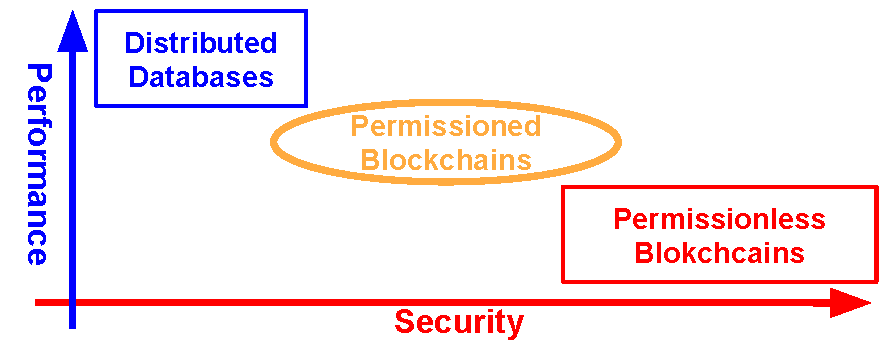
\includegraphics[width=0.99\textwidth]{diagram/twin/spectrum.pdf}
  \caption{Blockchains vs. distributed databases in the security-performance coordinate.}
  \label{diagram:twin:spectrum}
 \end{figure}


In earlier designs, a blockchain transaction is restricted to cryptocurrency and
the states are modeled as Unspent Transaction Outputs (UTXO).  For example,
Bitcoin~\cite{nakamoto2019bitcoin} and other similar altcoins use the UTXO
model.  Starting with Ethereum~\cite{web:ethereum}, blockchains support
\textit{smart contracts} which allow users to encode and execute arbitrary
Turing-complete computations on the ledger. The ledger states are modelled as
accounts instead of UTXO.
Other systems supporting smart contracts include Quorum, Parity and Hyperledger
Fabric~\cite{androulaki2018hyperledger}.  In these systems, a transaction on the
ledger takes the form of a contract invocation.
Transactions sequentially modify the system state based on their order in the
ledger, determined by the consensus protocol. A read-only transaction can be
carried out by any node, without undergoing the consensus and being included in
the ledger. We only consider blockchains that support smart contracts in this
paper, because earlier blockchains (without smart contracts) cannot support
database transaction workloads and thus cannot be compared with distributed
databases.

\textbf{Permissionless vs. Permissioned.} Blockchains can be broadly divided
into two categories: permissionless (or public), and permissioned (or private).
In the former, for example in Bitcoin and Ethereum, any node and user can join
the system in a pseudonymous manner. In the latter, for example in Fabric and
Quorum, the node and user must be authorized to join the system. With strong
membership control and action regulation, permissioned blockchains are more
suitable for enterprise applications and are particularly used in the financial
sector.
Figure~\ref{diagram:twin:spectrum} shows the security-performance tradeoffs in
blockchains. It highlights how permissionless blockchains can achieve stronger
security because they make no identity assumption. In contrast, permissioned
blockchains have weaker security because of the identity assumption, but can
achieve higher performance because they can employ consensus protocols with
higher efficiency. A more detailed discussion of permissionless versus
permissioned blockchain designs can be found
in~\cite{dinh2018untangling,dinh2017blockbench}.

\subsection{Distributed Databases}

Unlike blockchains, database systems have been around for decades.  Relational
databases, which support easy-to-use SQL language and intuitive ACID transaction
semantics, remained mainstream throughout the years. The recent demand of big
data processing and the fact that Moore's law is reaching its limit are major
factors behind the trend of scale-out database designs. Nowadays, both data and
computation are distributed over multiple nodes in order to achieve high
availability and scalability. Principles and techniques in designing and scaling
distributed databases are described in detail in~\cite{ozsu2011principles}.
Basically, there are two distinctive movements, namely NoSQL and NewSQL, under
this new distributed design direction.


\textbf{NoSQL vs. NewSQL.}
For scalability, many distributed databases abandon the complex relational model
and the strong ACID semantics.
These systems are referred to as {\em NoSQL}. They support more flexible data
models and weaker consistency.
% They adopt the BASE principle for their transaction semantics.
In the sense of the CAP theorem~\cite{gilbert2012perspectives}, these NoSQL
systems compromise consistency for the sake of availability.
A variety of their supported data models include key-value store (e.g,
Redis~\cite{carlson2013redis}, etcd~\cite{web:etcd}), document store (e.g,
CouchDB~\cite{anderson2010couchdb}), graph store (e.g,
Neo4J~\cite{vukotic2014neo4j}), column-oriented (e.g,
Cassandra~\cite{lakshman2010cassandra}) and so on.
The most lenient consistency model is eventual consistency which makes no
guarantees about the order of read and write operations.
Between eventual and strong consistency, researchers explore a variety of other
abstractions, such as sequential, causal, and PRAM consistency. They standardize
on the allowable operation behavior for the ease of reasoning.
Most NoSQL databases offer configurable options, where users can trade off
between performance and consistency.

The surge of NoSQL systems, however, does not obscure the cost in usability and
the increase in application complexity.  A new class of distributed database
systems, called {\em NewSQL}, aim to restore the relational model and ACID
semantics without sacrificing much scalability.
NewSQL has drawn attention since Google introduced
Spanner~\cite{corbett2013spanner}, the first NewSQL system. It was followed by a
few database vendors, such as CockroachDB~\cite{web:cockroach} and
TiDB~\cite{web:tidb}. In this paper, we consider both NoSQL and NewSQL systems.

\begin{figure}[tp]
    \centering
	\begin{subfigure}{0.5\textwidth}
	    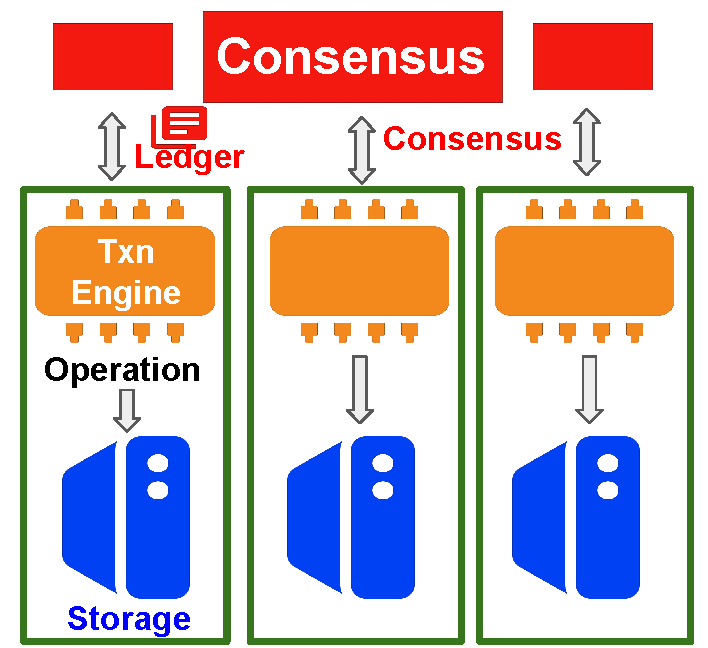
\includegraphics[width=0.9\textwidth]{diagram/twin/bc_arch.pdf}
	    % \caption{Blockchain architecture }
	    \caption{}
	\end{subfigure}%
	% \hspace{28mm}
	\begin{subfigure}{0.5\textwidth}
	    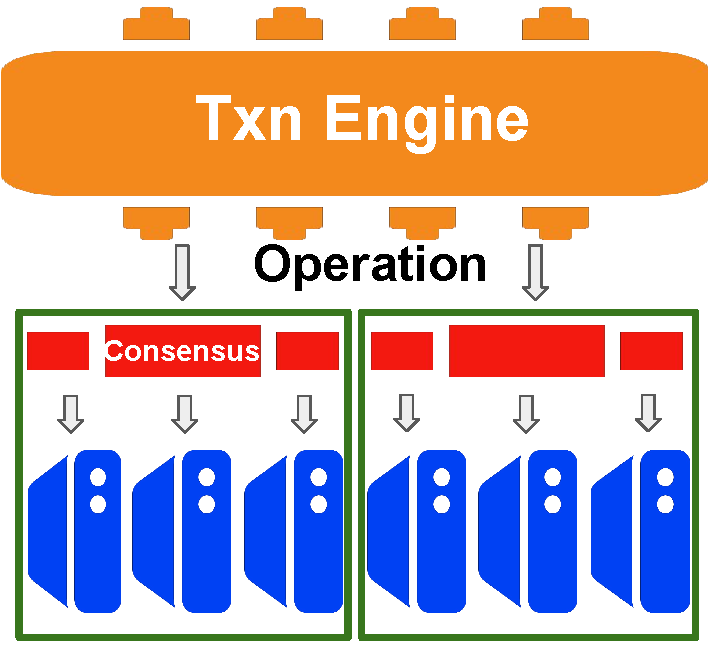
\includegraphics[width=0.9\textwidth]{diagram/twin/db_arch.pdf}
	    % \caption{Distributed database architecture}
	    \caption{}
	\end{subfigure}%
	\caption{Architecture of a blockchain and a distributed database}
    \subcaption*{(a) Blockchains first reach consensus on the transaction history, then commit their effects into the storage.
    (b) Distributed databases replicate at the storage layer.}
    \label{diagram:twin:arch}
\end{figure}

% \begin{landscape}
\begin{table}[tp]
	\centering
	\caption{Design choices in blockchains and distributed databases}
	\label{tab:twin:taxonomy}
	
	\resizebox{1.0\textwidth}{!}{%
	\begin{tabular}{l|ll}
	\toprule
	& \textbf{Blockchains} & \textbf{Distributed Databases} \\ 
	\hline
	\textbf{Replication} & \begin{tabular}[c]{@{}l@{}}Transaction replication \\
	Byzantine Fault Tolerant consensus \end{tabular} &
	\begin{tabular}[c]{@{}l@{}}State replication \\ 
	Crash Fault Tolerant consensus\end{tabular} \\ 
	\hline \textbf{Concurrency} & Serial execution & Concurrent execution \\ 
	\hline \textbf{Storage} & \begin{tabular}[c]{@{}l@{}}Append-only ledger
	abstraction \\ 
	Authenticated data structure: Merkle Tree, etc.\end{tabular} &
	\begin{tabular}[c]{@{}l@{}}Direct access without historical query \\
	Hardware-conscious index: PSL, FAST, etc.\end{tabular} \\ 
	\hline \textbf{Sharding} & \begin{tabular}[c]{@{}l@{}}Node-aware shard
	formation \\
	2PC and BFT-based replication\end{tabular} & \begin{tabular}[c]{@{}l@{}}Workload-aware shard formation \\ 
	2PC with centralized coordinator\end{tabular} \\
	\bottomrule
\end{tabular}
	}
\end{table}
% \end{landscape}


\section{Taxonomy}
\label{sec:twin:taxonomy}
% In this section, we present a distributed system taxonomy that illustrates the important design choices made
% by blockchains and distributed databases. We highlight how the differences are driven by the fact that these
% systems aim to achieve different goals: security for blockchains, and performance for databases.  

Table~\ref{tab:twin:taxonomy} compares the design choices of distributed databases and blockchains under each dimension in our taxonomy. 

\subsection{Replication}
Replication is the technique of storing copies of the data on multiple nodes called replicas. The key
challenge in such a system is to ensure consistency under failures.
In this section, we characterize blockchains and distributed databases by what they replicate, how they keep
the replicas consistent, and their failure models.

\subsubsection{Replication model}
The units of replication can be transactions or the read/write operations.
Figure~\ref{diagram:twin:arch} shows that blockchains replicate an ordered log of transactions (or ledger).  
Distributed databases replicate the ordered log of read and write operations on top
of the storage. The nodes in the database are oblivious to the transaction logic because they see only one
operation at a time. One consequence of this model is that the transaction manager which coordinates the
execution of a transaction must be trusted. In contrast, a blockchain does not have such trusted entity,
therefore it replicates the entire transaction so that its execution can be replayed by each participant node.

By replicating transactions, the ledger contain application-level information, such as transaction context,
client signature, execution timestamp, etc.,  making it easy to perform transaction verification.  Due to this
verifiability, blockchains are often used as a data and computing platform for mutually distrusting parties.
On the other hand, replicating storage operations means there can be more concurrency, because
operations can be replicated in different order but with the same effect on the storage.  

\subsubsection{Replication approach}
There are two main approaches to maintain consistency among replicas. The first
is primary-backup, which dedicates a replica as the primary which synchronizes
its states with backup replicas. This is adopted by many databases.
For example, Replex~\cite{replex} that uses chain replication.
Cassandra~\cite{lakshman2010cassandra} uses the client as the primary to
synchronize the replicas.

The second approach is state-machine replication, which essentially maintains an
ordered log of operations/transactions on each replica. Each replica starts at
the same initial state, then applies the operations/transactions in the log in
the same order. Many systems use {\em consensus protocols}, such as
Paxos~\cite{lamport2001paxos}, Raft~\cite{raft}, and
PBFT~\cite{castro1999practical}, for the replicas to agree on the ordered log.
Examples include Quorum~\cite{web:quorum}, TiDB~\cite{web:tidb},
Spanner~\cite{corbett2013spanner}.
Compared with the primary-backup, consensus protocols achieve the automatic
primary failover, by introducing the view change. That is, when the progress
halts, replicas may jointly agree to enter into a new epoch/view where a new
primary is elected.
Apart from the consensus, other systems rely on external services that provide a
distributed {\em shared log} abstraction, such as Kafka~\cite{web:kafka} and
Corfu~\cite{corfu}. Operations/transactions are appended to the log, and the
replicas, as clients of the log, apply them independently.
Examples of shared log systems include Fabric~\cite{web:fabric},
Hyder~\cite{hyder}, and Tango~\cite{tango}.

Primary-backup protocols are simpler, and can perform better than state-machine
replication, when the states are small and there are no failures. For example,
the chain replication protocol can spread the network cost more evenly among the
replicas than a consensus protocol, and it achieves better read
performance~\cite{replex}. Systems based on shared log are expected to perform
better than the ones based on consensus when there are no failures.  This is
because shared log decouples ordering from state replication, therefore it can
be optimized to have high throughput. Furthermore, while the throughput of a
consensus protocol decreases with more replicas, the throughput of a shared log
system is expected to remain constant until the number of log consumers exceeds
the capacity of the log producers~\cite{corfu}. 
 
\subsubsection{Failure model}
\label{sec:twin:taxonomy:replication:failure}
Replication protocols are complex because they need to maintain consistency
under failure. Under the crash failure model, in which nodes only fail by
crashing, the protocols need to tolerate hardware and software failures. Under
the Byzantine failure model, in which nodes fail arbitrarily, the protocols need
to tolerate any software and hardware failures, as well as any malicious
behavior. This model is suitable for achieving security, since it considers
attacks that fully compromise some nodes in the system.

An orthogonal dimension to the node failure model is the network assumption. The
network is {\em synchronous} when the network delay is bounded and known. It is
{\em asynchronous} when the network delay is unbounded. Protocols that tolerate
crash failures, or CFT, require $f+1$ replicas to tolerate $f$ failures under
the synchronous network model~\cite{budhiraja1993primary}, and $2f+1$ under the
asynchronous network model~\cite{raft,lamport2001paxos}. Protocols that tolerate
Byzantine failure, or BFT, require $2f+1$ and $3f+1$ replicas to tolerate $f$
failures under the synchronous and asynhronous network models,
respectively~\cite{castro1999practical, yin2019hotstuff,buchman2016tendermint}.

Databases assume the crash failure model, since they are considered internal
systems which are not subject to security attacks. For example,
Spanner~\cite{web:spanner} uses Paxos~\cite{lamport2005generalized}, a CFT
protocol.  Permissioned blockchains support both failure models. For example,
Quorum provides implementations for both Raft~\cite{raft}, a CFT protocol, and
IBFT, a BFT protocol. These systems allow applications to make different
tradeoffs between security and performance.
Public blockchains, on the other hand, ubiquitously adopt BFT protocols because they admit
any nodes to the system. In particular, PoW protocols are often used because
they address one fundamental problem in the public settings: a node can have
many identities. In PoW, a node's probability of solving a computational puzzle,
thereby reaching consensus and gaining rewards, is proportional to its physical
resources which are difficult to forge.

\begin{figure}
    \centering
    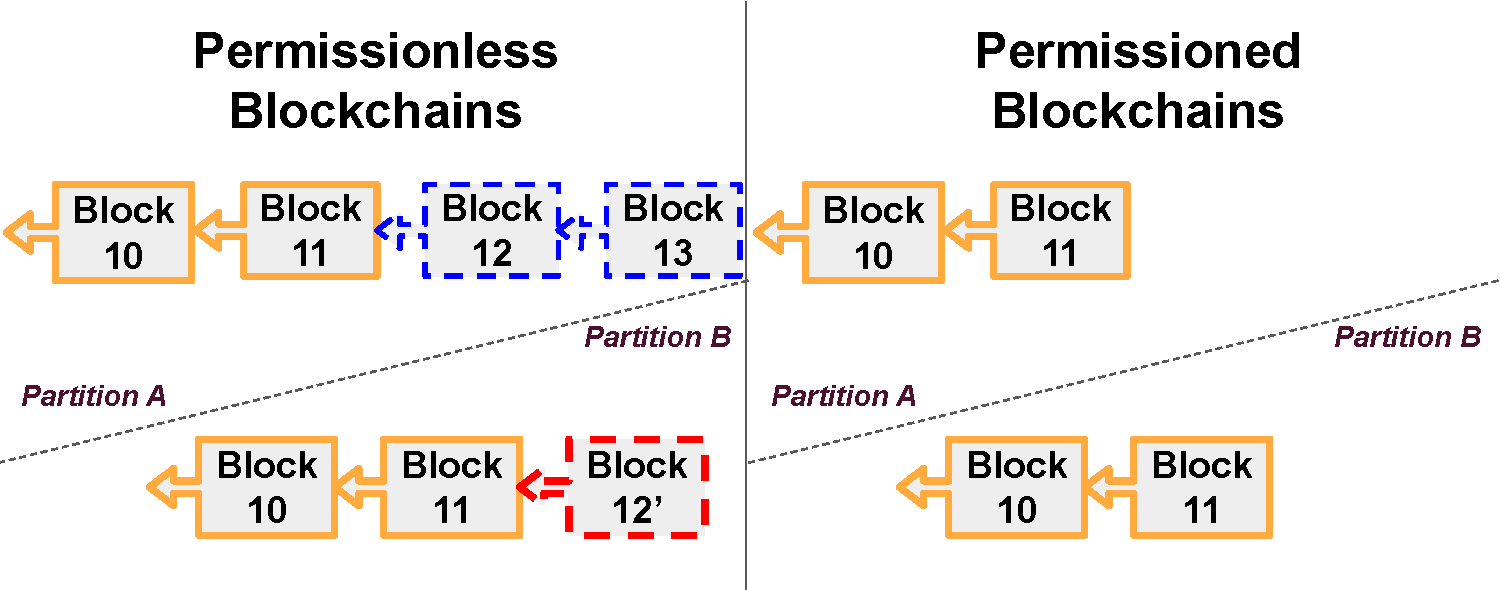
\includegraphics[width=0.975\textwidth]{diagram/twin/fork.pdf}
	\caption{Permissonless vs. permissioned blockchains during the asynchronous period} 
	\subcaption*{When the network partition occurs after Block 11, The former keep appending blocks in each partition, while
    the later become unavailable but remain consistent.}
    \label{diagram:twin:fork}
\end{figure}

In an asynchronous network and under failures, the FLP
theorem~\cite{fischer1982impossibility} rules out any deterministic consensus
protocol that can achieve both safety and liveness. Public blockchains choose
liveness over safety, meaning that the systems remain available under network
partitions, but these partitions may be in disagreement which takes the form of
forks, as shown in Figure~\ref{diagram:twin:fork}.
Here, availability refers to the system's behavior, that is, new
blocks are appended to the ledger. Individual transactions may be
censored and excluded from the blockchain.

PoW protocols have low throughputs mainly due to the resource
requirements~\cite{dinh2017blockbench}.
CFT protocols have better performance than BFT protocols, because the former
incur $O(N)$ network cost, whereas the latter incur $O(N^2)$, where $N$ is the
number of nodes. As a result, BFT protocols do not scale to a large number of
nodes, and their performance is more sensitive to network conditions at scale.
Specifically, when $N$ is large, BFT protocols are more likely to enter view
change --- an expensive phase of the protocol for replacing the current leader.


\subsection{Concurrency}

Concurrency refers to the extent to which transactions are executed at the same
time. There are two choices: transactions are executed either serially (or
sequentially), or concurrently. Most blockchains support only serial execution,
while distributed databases employ sophisticated concurrency control mechanisms
to extract as much concurrency as possible.

There are two reason behind blockchains' lack of support for concurrency. First,
serial execution may not affect the overall performance because transaction
execution is often not the bottleneck~\cite{dinh2017blockbench}.   For
example, in Bitcoin, the consensus protocol may take several minutes to
complete, which is the block interval required by the protocol, whereas the
transaction execution, which invokes the Bitcoin script to validate a
cryptocurreny flow, can be done in milliseconds. Second, serial execution means
the behavior of smart contracts is deterministic when the transaction execution
is replicated over many nodes. The benefit of determinism is that it is easy to
reason about the states of the ledger.

Unlike blockchains, concurrency remains a major research topic in databases, as
it is the main source of performance improvement. The challenge in extracting
concurrency is to ensure the correctness of the concurrent execution. In fact,
there is a wide range of isolation
levels~\cite{computer1986american,bailis2013highly} which make different
tradeoffs between correctness and performance. Most production-grade databases
today offer more than one isolation level.

We observe that recent blockchains are adopting some simple concurrency
techniques often found in databases. In Hyperledger Fabric, for example,
transactions are simulated (executed) in parallel against the ledger states
before being sent for ordering. During the later commit phase, the system uses a
simple optimistic concurrency control to achieve serializability which aborts
transactions whose simulated states are stale. More established techniques to
reduce abort have also been proposed~\cite{sharma2019blurring,
ruan2020transactional}.

\subsection{Storage}

In this section, we describe how blockchains and distributed databases build
different models and data structures for storage.

\subsubsection{Storage model}
Storage can be built upon the latest states only, amenable for mutation, or upon
all historical information, amenable for appending.
The storage in distributed databases only exposes direct access to up-to-date
records. In databases without explicit provenance support, historical data is
maintained in limited forms, for example as write-ahead logs.
We note that such logs are used primarily for failure recovery, and they are
periodically pruned.
Blockchains, besides the state storage, additionally expose an append-only
ledger abstraction.
The ledger, a chain of blocks, records historical transactions and the changes
made to the global states.
We note that such a ledger is hash protected to conserve historical integrity.
Some blockchains allow applications to access only the latest states, for
example, Hyperledger Fabric v0.6.
Recently, novel blockchain-tailored storage systems have been proposed to enable
access to any historical states during smart contract
execution~\cite{ruan2019fine}.

\subsubsection{Index}
Indexes play an instrumental role on the state storage to facilitate data
access.
Apart from the performance consideration, some security-oriented systems
additionally rely on the index to compute a digest, which uniquely identifies
the state contents.
Distributed databases are more concerned by performance, i.e., any small
optimization on the index can translate to a significant improvement in
performance. Modern indexes are designed to be hardware-conscious in order to
extract the most efficiency from the hardware. For example, in-memory databases
abandon the disk-friendly B-tree structure for other structures such as
FAST~\cite{kim2010fast} and PSL~\cite{xie2017parallelizing} which are designed
for better cache utilization and multi-core parallelism.

To compute the content-unique digest, blockchains employ an authenticated data
structure, such as the Merkle tree index, to provide integrity protection on top
of the state storage.
For example, Ethereum uses a prefix trie, named Merkle Patricia Trie
(MPT)~\cite{web:mpt}. In MPT, the states are stored in the leaves. The states
with a common key prefix are organized under the same branch. Each node is
associated with the cryptographic hash of its content in the storage engine,
such that the root hash represents the complete global states. The access path
serves as the integrity proof for the retrieved value. Older versions of
Hyperledger Fabric use a Merkle Bucket Tree (MBT) in which the size of the tree
is fixed.
Unlike the ledger abstraction which is ubiquitous in blockchains, we note that
not all blockchains adopt the authenticated data structure for the state
organization. For example, Hyperledger Fabric abandons this design from version
1 onwards.	


\subsection{Sharding}

Sharding is a common technique in distributed databases for achieving
scalability, in which data is partitioned into multiple shards. Although it has
been studied extensively in databases, sharding has only recently been
introduced to blockchains to harness concurrency across shards. In
this section, we discuss two key challenges in any sharded system, that are (i)
how to form a shard, and (ii) how to ensure atomicity for cross-shard
transactions.

\subsubsection{Shard formation}
A shard formation protocol determines which nodes and data go to which shard.
The security of blockchains depends on the assumption that the number of
failures is below a certain threshold. The shard formation protocol must,
therefore, ensure that the assumption holds for every shard.
In particular, the shard size must be large enough so that the fraction of
Byzantine nodes is small.
Furthermore, the attacker must not be able to influence the shard assignment,
otherwise, it could reserve enough resources for one shard to break the security
assumption. State-of-the-art sharded blockchains have different approaches. For
example, Elastico uses PoW for shard formation~\cite{luu2016secure}, while
 the recent version of Ethereum uses Proof-of-Stake to select
validators for each shard~\cite{web:eth2}.
OmniLedger~\cite{kokoris2018omniledger} employs a complex cryptographic
protocol, while AHL~\cite{dang2018towards} uses trusted hardware.
These protocols are secured against Sybil attacks, and executed
regularly, in the form of shard reconfiguration, to guard against adaptive
attackers.

The goal of sharding in distributed databases is scalability. As such, the
systems aim to assign data to shards in a way that optimizes the performance of
certain workloads. In practice, they offer a variety of partitioning schemes,
for example, hash partitioning and range partitioning, so that users can select
the most suitable for their workloads. Some systems, for instance,
Cassandra\cite{lakshman2010cassandra}, even allow users to specify workload
distributions so that data can be partitioned in a locality-aware manner. Unlike
blockchains, shard reconfiguration is not necessary for databases, unless when
there are significant changes in the workload distribution.

\subsubsection{Atomicity}
Sharding introduces the problem of transaction atomicity when a transaction
touched data in multiple shards.
Atomicity requires a cross-shard transaction to either commit or abort in all
shards. In databases, this problem is addressed by the two-phase commit (2PC)
protocol. This protocol requires a dedicated transaction coordinator that must
be trusted, but may fail and leave the transaction blocked forever. A recent
work proposed Parallel Commit to reduce the commit duration to a single round
trip~\cite{taft2020cockroachdb}.

Sharded blockchains face additional challenges in ensuring atomicity because the
coordinator cannot be trusted under the Byzantine failure model.
To overcome this, Eth2 introduces a separate chain running Casper
consensus~\cite{buterin2017casper}, called Beacon Chain, that coordinates
cross-shard transactions~\cite{web:eth2}.
Similarly, \cite{dang2018towards,herlihy2019cross} propose to implement the 2PC
coordinator as a state machine in a shard that runs a BFT protocol. The BFT
protocol ensures that the shard is less vulnerable to attacks and does not
become a point of failure.
Any cross-shard transaction must involve this 2PC BFT replicated state machine
to ensure atomicity.
The consensus liveness guarantees the high availability of the coordinator,
therefore mitigating the blocking problem.
But the Byzantine setup in blockchains imposes considerable overhead to the 2PC
process.

\subsection{Fusion of Blockchains and Databases}
The taxonomy above provides a comprehensive description of the design space of
distributed transactional systems. This taxonomy helps in illustrating the
similarities and differences between blockchains and distributed databases. It
also serves as a principled framework for understanding the recently emerging
hybrid blockchain-database systems. In this section, we discuss how these
systems fit into the design space. We provide a deeper analysis of their
performance in Chapter~\ref{sec:twin:exp:hybrids}.

\textbf{Out-of-the-blockchain Databases.} One approach toward a hybrid design is
to start with a blockchain (or a blockchain-like system) and build database
features on top of it. Examples of this approach include
BlockchainDB~\cite{el2019blockchaindb}, Veritas~\cite{veritas}, and
FalconDB~\cite{peng2020falcondb}, which provide shared and verifiable databases
for multiple distrusting parties.
They use blockchains as an integrity-protected storage, and build other database
components on top of it.
In these systems, replication is transaction-oblivious, with duplicated states,
logs, and meta-data.
BlockchainDB replicates storage operations and uses PoW for
consensus. It inherits the authenticated state organization from the underlying
blockchain and employs multiple blockchains for storage. Therefore, it is
amenable to sharding. However, transactions are executed sequentially within
each shard.
FalconDB and Vertias also adopt storage-based replication, but use
Tendermint~\cite{buchman2016tendermint} for consensus and Kafka~\cite{web:kafka}
as the shared log, respectively.
They use a similar optimistic concurrency control mechanism as Fabric. FalconDB
outsources the authentication task to IntegriDB~\cite{zhang2015integridb}, which
enables a light-weight client to produce a proof without holding the entire
ledger. Veritas relies on trusted verifiers for the state integrity.

\textbf{Out-of-the-database Blockchains.} Another hybrid design approach is to
start with a database, then add blockchain features to it. Examples of this
approach include BigchainDB~\cite{mcconaghy2016bigchaindb}, Blockchain
Relational Database (BRD)~\cite{BlockchainMeetsDatabase}, and
ChainifyDB~\cite{schuhknecht2019chainifydb}. In these systems, each node has its
own database and executes transactions on its database according to a global
order achieved through consensus.
These systems adopt the transaction-based replication model where the
ledger serves as a secure shared log that stores transactions.
The nodes execute the same sequence of transactions, but on different local
databases.
In particular, BRD uses PostgreSQL~\cite{postgres} and the transactions contain
invocation contexts of stored procedures. BigchainDB uses
MongoDB~\cite{web:mongodb}, thus its transactions are in JSON format.
ChainifyDB allows heterogeneous relational databases, and transactions are in
the form of standardized SQL statements.
ChainifyDB uses a Kafka broker to share logs for efficiency. In contrast,
BigchainDB uses the Tendermint consensus protocol which tolerates Byzantine
failures at the expense of performance.
BRD jointly uses Kafka~\cite{web:kafka} and BFT-SMaRt~\cite{bftsmart}, an
implementation of PBFT.
These systems inherit the concurrency support of their underlying databases,
with serializable constraints according to the ledger order. However, these
systems do not protect the local states with Merkle trees and only rely on the
integrity protection of the ledger.
Finally, these systems do not support sharding.

In summary, out-of-the-database blockchains retain many design choices of
distributed databases, as their main goal is performance. In contrast,
out-of-the-blockchain databases inherit many design choices of blockchains, as
their main goal is security.

\subsection{Discussion}

Table~\ref{tab:twin:systems} summarizes some representative transactional systems and
their design choices based on our proposed taxonomy.
We only consider blockchains with generic smart contracts and NoSQL databases
with key-value data model.
We exclude permissionless blockchains from our quantitative analysis, as their
security-performance tradeoffs have been extensively
studied~\cite{gervais2016security}.
One can observe from Table~\ref{tab:twin:systems} that the hybrid systems, just like
permissioned blockchains, share some security-oriented design choices with
blockchains and some performance-oriented design choices with databases.

\begin{landscape}

	\begin{table*}[tp]
		\centering
		\caption{System comparison based on our taxonomy }
		\subcaption*{ 
		For each hybrid system, we mark their security-oriented designs with red and performance-oriented designs with blue.
		}
		\label{tab:twin:systems}
		
		\definecolor{highlighted}{rgb}{0.7, 0.75, 0.71}
	
		\newcommand{\security}[1]{{\color{red}{#1}}}
		\newcommand{\performance}[1]{{\color{blue}{#1}}}
	
	
		\resizebox{1.5\textwidth}{!}{%
		\begin{tabular}{cclcccccc} 
			\toprule
			\multirow{2}{*}{\textbf{Category}} & \multirow{2}{*}{\textbf{System}} & \multicolumn{3}{c}{\textbf{Replication} }                                                                                                                                                  & \multirow{2}{*}{\textbf{Concurrency} } & \multicolumn{2}{c}{\textbf{Storage} } & \multirow{2}{*}{\begin{tabular}[c]{@{}c@{}}\textbf{Sharding }\\\textbf{ Support (2PC)} \end{tabular}}  \\
									  &                          & \begin{tabular}[c]{@{}l@{}}Replication \\ Model \end{tabular} & \begin{tabular}[c]{@{}c@{}}Replication \\Approach \end{tabular} & \begin{tabular}[c]{@{}c@{}}Failure Model\\(Consensus Protocol) \end{tabular} &                                        & Ledger Abstraction & Index(Storage Engine)                 &                                                                                                  \\
	
			\midrule
			\multirow{2}{*}{\makecell{Permissionless \\ Blockchains}} & Ethereum~\cite{web:ethereum} & Txn-based & Consensus & BFT(PoW) & Serial & \cmark & LSM Tree(LevelDB)+MPT & \xmark(\xmark)\\
	
			\cdashline{2-9} \\
			& Eth2~\cite{web:eth2} & Txn-based & Consensus & BFT(PoS + Casper) & Serial (in each shard) & \cmark & LSM Tree(LevelDB)+MPT & \cmark(\xmark)\\
	
			\midrule
	
			\multirow{5}{*}{ \makecell{Permissioned \\ Blockchains}} & \cellcolor{highlighted}Quorum v2.2~\cite{web:quorum} &  \cellcolor{highlighted}Txn-based &  \cellcolor{highlighted}Consensus &  \cellcolor{highlighted}Raft(CFT)/IBFT(BFT) &  \cellcolor{highlighted}Serial &  \cellcolor{highlighted}\cmark & \cellcolor{highlighted} LSM Tree(LevelDB)+MPT &  \cellcolor{highlighted}\xmark(\xmark) \\
	
			\cdashline{2-9} \\
	
			&\cellcolor{highlighted} Fabric v2.2~\cite{web:fabric} &\cellcolor{highlighted} Txn-based &\cellcolor{highlighted} Shared log &\cellcolor{highlighted} CFT(\textit{Orderer} with Raft) &\cellcolor{highlighted} \makecell{Concurrent Execution \\ Serial Commit}&\cellcolor{highlighted} \cmark &\cellcolor{highlighted} LSM Tree(LevelDB) &\cellcolor{highlighted} \xmark(\xmark) \\
	
			\cdashline{2-9} \\
	
			& Fabric v0.6~\cite{web:fabric06} & Txn-based & Consensus & BFT(PBFT) & Serial & \cmark & \makecell{LSM Tree(RocksDB) \\ + MBT} & \xmark(\xmark)
			\\
	
			\cdashline{2-9} \\
			& EOS~\cite{web:eos} & Txn-based & Consensus & BFT(DPoS) & Serial & \cmark & B-tree(MongoDB) &  \xmark(\xmark) \\
	
			\cdashline{2-9} \\
	
			& \multirow{2}{*}{FISCO BCOS~\cite{web:fisco}} & \multirow{2}{*}{Txn-based} &  Consensus & CFT(Raft) & \multirow{2}{*}{Serial} & \multirow{2}{*}{\cmark} & \multirow{2}{*}{\makecell{LSM Tree(LevelDB) \\+MPT}} & \multirow{2}{*}{\xmark(\xmark)} \\
			& &  & & BFT(PBFT) & &  &  &  \\
	
			\midrule
			\multirow{3}{*}{\makecell{NewSQL \\ Databases}} & \cellcolor{highlighted} {TiDB v4.0~\cite{web:tidb}} & \cellcolor{highlighted}{Storage-based} & \cellcolor{highlighted}Consensus &\cellcolor{highlighted} CFT(Raft) &\cellcolor{highlighted} Concurrent &\cellcolor{highlighted} \xmark &\cellcolor{highlighted} LSM Tree(TiKV) &\cellcolor{highlighted}  \cmark(\cmark) \\
	
			\cdashline{2-9} \\
			 & CockroachDB~\cite{web:cockroach} & Storage-based & Consensus & CFT(Raft) & Concurrent & \xmark & LSM Tree(RocksDB) &  \cmark(\cmark) \\
			\cdashline{2-9} \\
			 & Spanner~\cite{web:spanner} & Storage-based & Consensus & CFT(Paxos) & Concurrent & \xmark & LSM Tree &  \cmark(\cmark) \\
	
			\cdashline{2-9} \\
			 & H-store~\cite{kallman2008h} & Storage-based & Primary-backup & CFT & Concurrent & \xmark & B Tree &  \cmark(\cmark) \\
	
			\midrule
			\multirow{3}{*}{\makecell{NoSQL \\ Databases}} &\cellcolor{highlighted} Etcd v3.3~\cite{web:etcd} &\cellcolor{highlighted} Storage-based &\cellcolor{highlighted} Consensus &\cellcolor{highlighted} CFT(Raft) &\cellcolor{highlighted} Serial &\cellcolor{highlighted} \xmark &\cellcolor{highlighted} B Tree(BoltDB) & \cellcolor{highlighted} \xmark(\xmark) \\
	
			\cdashline{2-9} \\
			& Cassandra~\cite{web:cassandra}& Storage-based & Primary-backup & CFT & Concurrent & \xmark & LSM Tree &  \cmark(\xmark) \\
			\cdashline{2-9} \\
			& DynamoDB~\cite{web:dynamodb} & Storage-based & Primary-backup & CFT & Concurrent & \xmark & B Tree &  \cmark(\xmark) \\
	
			\midrule
			\multirow{3}{*}{\makecell{Out-of-the \\ Blockchain \\ Databases}} & BlockchainDB~\cite{el2019blockchaindb} & \performance{Storage-based} & Consensus & \security{BFT(PoW)} & \security{Serial (in each shard)} & \security{\cmark} & \security{\makecell{LSM Tree(LevelDB)\\+MPT}} &  \cmark(\xmark) \\
	
			\cdashline{2-9} \\
			& Veritas~\cite{veritas} & \performance{Storage-based} & Shared log& \performance{CFT(Kafka)} & \performance{\makecell{Concurrent Execution \\ Serial Commit}} &  \security{\makecell{\cmark}} & \performance{Skip List(Redis)} &  \xmark(\xmark) \\
	
			\cdashline{2-9} \\
			& FalconDB~\cite{peng2020falcondb} & \performance{Storage-based} & Consensus & \security{BFT(Tendermint)} & \performance{\makecell{Concurrent Execution \\ Serial Commit}} &  \security{\makecell{\cmark }} & \security{\makecell{B Tree(MySQL)\\+Merkle Tree(IntegriDB)}} &  \xmark(\xmark) \\
	
			\midrule
			\multirow{3}{*}{\makecell{Out-of-the \\ Database \\ Blockchains}} & \makecell{Blockchain Relational\\
		Database (BRD)~\cite{BlockchainMeetsDatabase}} & \security{Txn-based} & \makecell{Shared log} & \makecell{\performance{CFT(Kafka)} \\ \security{BFT(BFT-SMaRt)}} & \performance{Concurrent} & \security{\cmark} & \performance{\makecell{B Tree(PostgreSQL)}} &  \xmark(\xmark) \\
	
			\cdashline{2-9} \\
			& ChainifyDB~\cite{schuhknecht2019chainifydb} & \security{Txn-based} & Shared log& \performance{CFT(Kafka)} & \performance{Concurrent} &  \security{\cmark} & \performance{\makecell{B Tree\\(MySQL/PostgreSQL)}} &  \xmark(\xmark) \\
	
			\cdashline{2-9} \\
			& BigchainDB~\cite{mcconaghy2016bigchaindb} & \security{Txn-based} & Consensus & \security{BFT(Tendermint)} & \performance{Concurrent} &  \security{\cmark} & \performance{B Tree(MongoDB)} &  \xmark(\xmark) \\
	
			\bottomrule
			\end{tabular}
		}
	\end{table*}

\end{landscape}

\section{Experimental Setup}
\label{sec:twin:setup}
\subsection{Systems}

We select four representative systems: two permissioned blockchains, namely Quorum~\cite{web:quorum} and Hyperledger Fabric~\cite{web:fabric}, and two distributed databases, namely TiDB~\cite{web:tidb} and etcd~\cite{web:etcd}.
Quorum represents order-execute blockchains, while Fabric represents execute-order-validate blockchains. 
They also employ different replication approaches, as shown in Figure~\ref{diagram:literature:execution}.
Fabric employs an external ordering service while Quorum relies on Raft consensus.

Quorum is a fork of \textit{geth}, the Golang implementation of Ethereum. 
Quorum replaces the original Proof of Work (PoW) of Ethereum with a CFT protocol, namely Raft, and a BFT protocol called
Istanbul BFT (IBFT). However, it inherits Ethereum Virtual Machine (EVM) to invoke smart contracts.

Fabric is featured for its modularized design. 
In particular, a node role is separated into \textit{orderer} and \textit{peer}, as also detailed in Figure~\ref{diagram:literature:execution}.

TiDB~\cite{web:tidb} and etcd~\cite{web:etcd} represent NewSQL and NoSQL
distributed databases, respectively.
TiDB consists of three independent modules, namely Placement Driver for
coordinating cluster management, TiKV as the replicated key-value storage, and
TiDB-server for parsing and scheduling SQL queries in a stateless manner. TiDB
only supports snapshot isolation.
Etcd provides a simple key-value data model with relaxed transactional
restrictions but focuses on the tradeoff between availability and consistency.
Similar to blockchains, etcd employs a single consensus instance to sequence all
the requests.
Without sharding, etcd fully replicates the data on each node.
We also benchmarked CockroachDB~\cite{web:cockroach}, another NewSQL database. Since it exhibits similar performance trends as TiDB, we decide to omit it in this paper. 

% \begin{figure}[tp] 
% 	\centering
% 		\begin{subfigure}{0.99\textwidth}
% 			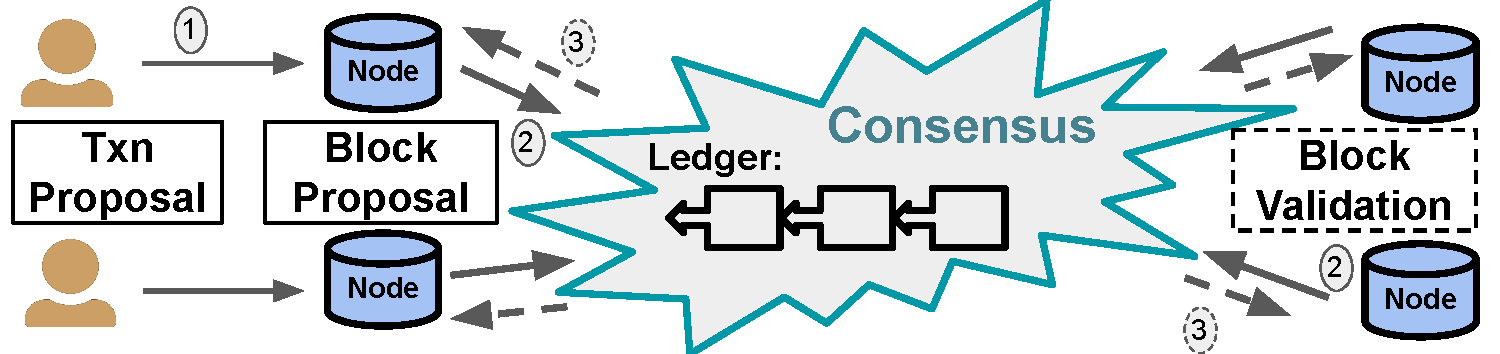
\includegraphics[width=0.99\textwidth]{diagram/twin/quorum_arch.pdf}
% 			\caption{Quorum transaction lifecycle}
% 			\label{chart:twin:quorum-arch}     
% 		\end{subfigure}
% 		\begin{subfigure}{0.99\textwidth}
% 			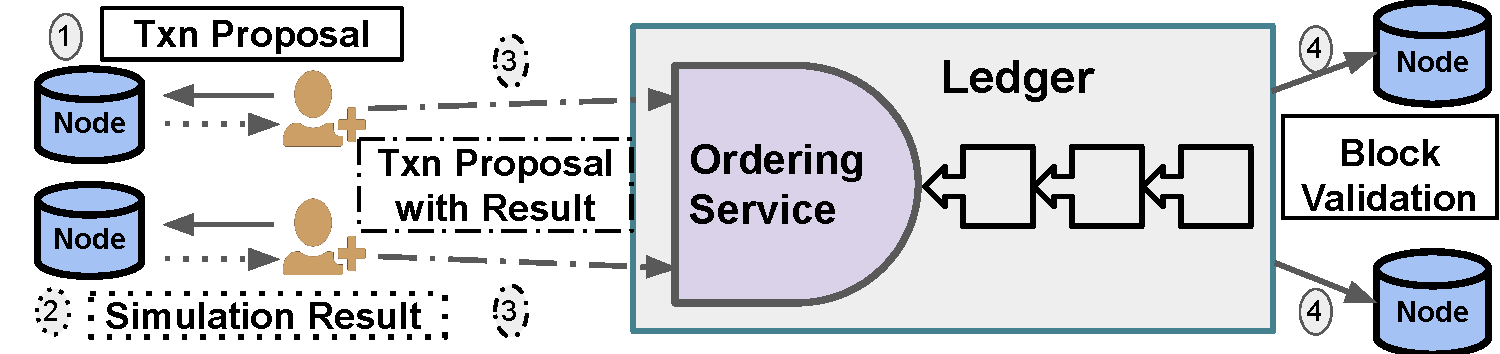
\includegraphics[width=0.99\textwidth]{diagram/twin/fabric_arch.pdf}
% 			\caption{Fabric transaction lifecycle}
% 			\label{chart:twin:fabric-arch}
% 		\end{subfigure}
% 	\caption{Transaction execution in Quorum vs. Fabric.}
% 	\subcaption*{In Quorum, a node
% 	assembles pre-executed transactions into blocks before running the consensus.
% 	In Fabric, a client collects simulation results and endorsements from peer
% 	nodes to form a transaction. Orderer nodes order the transactions and batch
% 	them into blocks, which are then pulled by the peer nodes for independent
% 	validation and commit.} 
% 	\label{chart:twin:fabric_vs_quorum}
% \end{figure}

\subsection{Setup}
For a fair comparison, we run all systems in full replication mode where each
node has a complete copy of the states. In particular, for Fabric the
endorsement policy is set such that a transaction is executed and endorsed by
all peers. For TiDB, we set the replication factor to be the same as the number
of nodes. In other words, even though TiDB partitions data to multiple
shards and manages the shards separately, each node has a copy of the entire
system state. We configure Quorum and Fabric to use Raft, a CFT consensus.
For Fabric, we fix the number of orderers to three while scaling the peers.
For TiDB, we scale all its modules with the number of nodes.

Unless otherwise specified, we use YCSB and Smallbank workloads in our
experiments. The experiment parameters for YCSB are summarized in
Table~\ref{tab:twin:parameter} with the default values underlined.

\begin{table}
	\centering
	\caption{Experiments parameters}
	\label{tab:twin:parameter}
	\begin{tabular}{@{}ll@{}}
	\toprule
	\textbf{Variable}               & \textbf{Values}               \\
	\midrule
	Record size (Byte)               & 10, 100, \underline{1000}, 5000          \\
	Zipfian coefficient $\theta$       & \underline{0.0}, 0.2, 0.4, 0.6, 0.8, 1.0 \\
	\# of transaction operations & \underline{1}, 2, 4, 6, 8, 10            \\
	\# of nodes & 3, \underline{5}, 7, 11, 15, 19            \\
	\bottomrule
	\end{tabular}
\end{table}

\begin{figure}
	\centering
	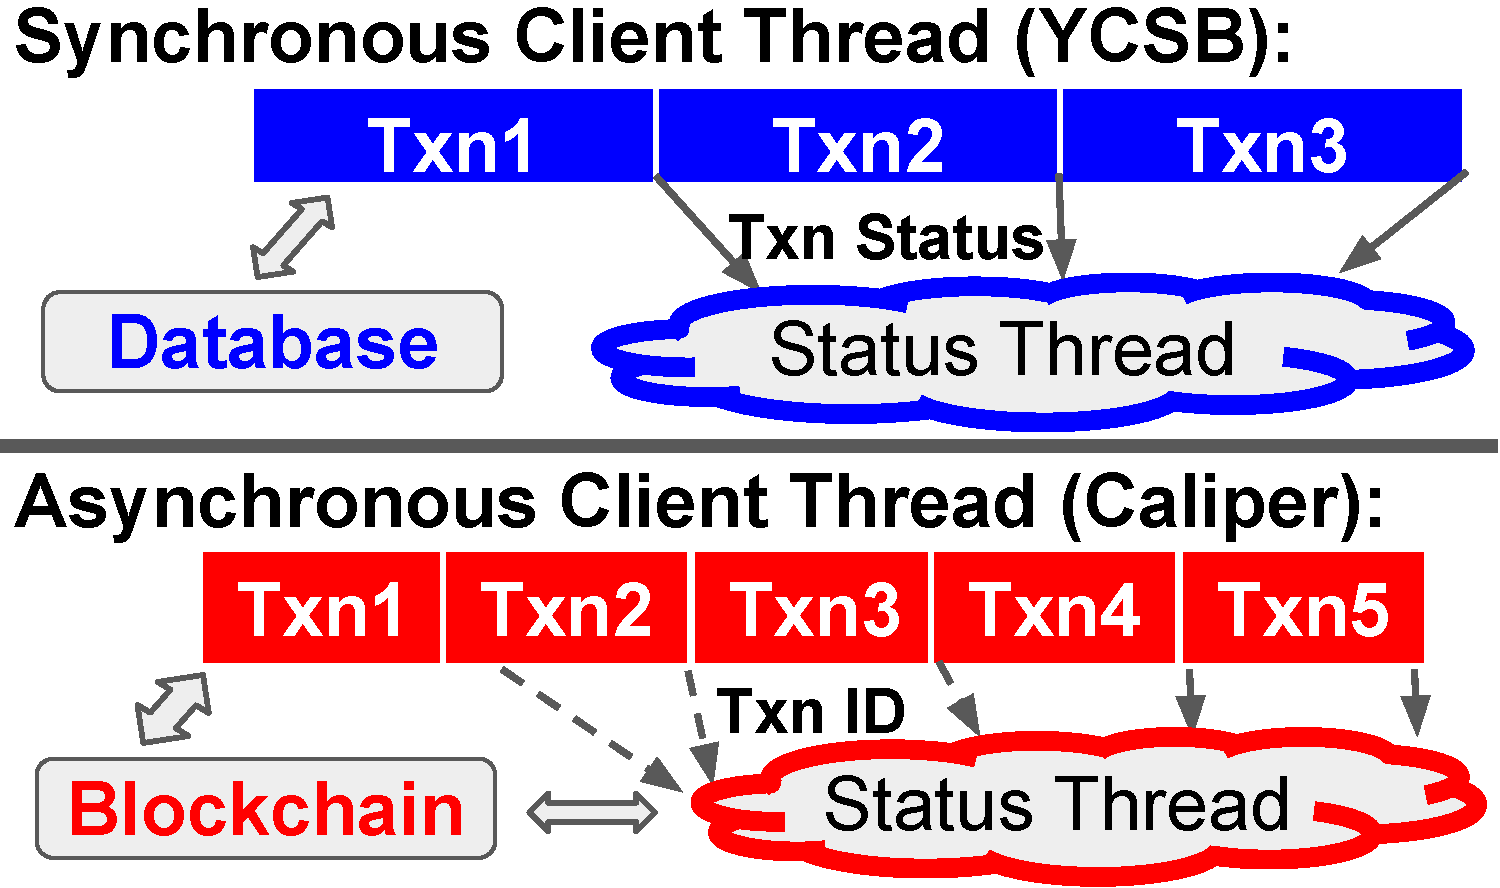
\includegraphics[width=0.8\textwidth]{diagram/twin/driver_diff.pdf}
	\caption{Differences between synchronous and asynchronous drivers. }
	\subcaption*{Asynchronous drivers can issue more transactions, as they do not have to wait for their completion, as opposed to the synchronous ones.}
	\label{diagram:twin:driver_diff} 
\end{figure}

\subsection{Benchmark Driver}
We note that existing benchmark drivers for databases are synchronous (or closed-loop), meaning that a next
request is sent only after the current request is completed. In contrast, blockchain benchmark
drivers, such as Hyperledger Caliper and BLOCKBENCH driver~\cite{dinh2017blockbench}, are asynchronous (or
open-loop) in which a new request is sent as soon as the current request is acknowledged by a
node in the blockchain. 
Figure~\ref{diagram:twin:driver_diff} illustrates the difference between the two types of drivers. 
In a synchronous driver, a separate status thread is responsible for computing statistics. In an
asynchronous driver, the status thread needs to keep track of the outstanding requests and to periodically poll
the blockchain for newly completed requests.

Asynchronous drivers are suitable for blockchains because of the long request latency which requires a large number of outstanding requests to saturate the system. In other words, benchmarking a blockchain with synchronous drivers would require many nodes to run the driver. 
To verify this, we implement a synchronous YCSB driver for Fabric using its Java SDK.  
Our results show that the synchronous driver severely underestimates Fabric's performance, even with a large number of client-side requests issued.

For the database experiments we use the open-source driver for YCSB workload~\cite{web:ycsb} and 
the OLTPBench~\cite{difallah2013oltp} driver for Smallbank workload.  Both Fabric and Quorum are
benchmarked using Caliper~\cite{web:caliper}. We note that although there are differences in the types of
drivers for benchmarking blockchains and databases, they alone do not account for the large performance gap
reported in the following section. 

\section{Result and Analysis}
\label{sec:twin:exp}
We first summarize the main findings, then provide the detailed experimental analysis. Based on these findings,
we propose an empirical framework that compares the performance of recent hybrid blockchain-database systems.
The framework not only explains the performance differences in existing systems, but it is also useful for
understanding future hybrid systems.

\begin{itemize}
  \item \textbf{Peak performance.} The performance gap between blockchains and distributed databases is large. However, the gap is not as significant as previously reported.
  \item \textbf{Replication. }
    The transaction-based replication model restricts concurrency, which limits the impact of different
	replication approaches and failure models on the system's peak performance. 
  \item \textbf{Concurrency.} Execute-order-validate blockchains have low performance under workloads with high contention and constraints.
  The impact of workloads on the performance is prominent in NewSQL databases, where concurrency is
  on top of replication.
  \item \textbf{Storage. } The ledger abstraction in blockchains incurs significant storage overhead. On the
  other hand, the overhead needed to guarantee state tamper evidence is small.
  \item \textbf{Sharding. } The performance of sharded blockchains is far behind that of distributed
  databases, due to the security requirements on shard formation and periodic reconfiguration.
\end{itemize}

\subsection {Peak Performance}
\subsubsection{YCSB}

\begin{figure}[tp]
	\centering
    \begin{subfigure}{0.45\textwidth}
        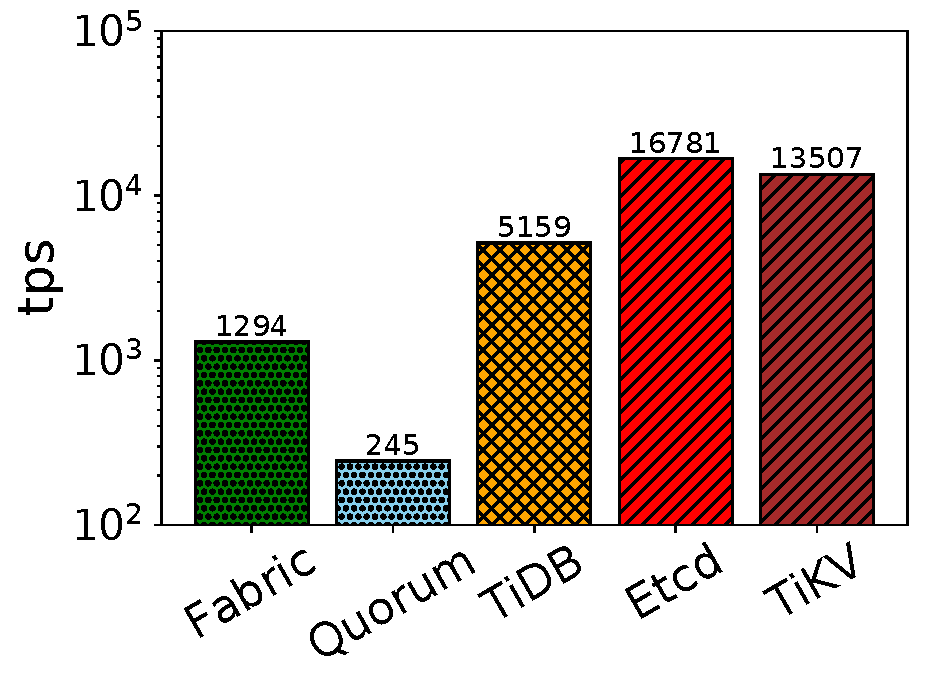
\includegraphics[width=0.99\textwidth]{chart/twin/ycsb-update.pdf}
        \caption{Update}
    \end{subfigure}
    \begin{subfigure}{0.45\textwidth}
        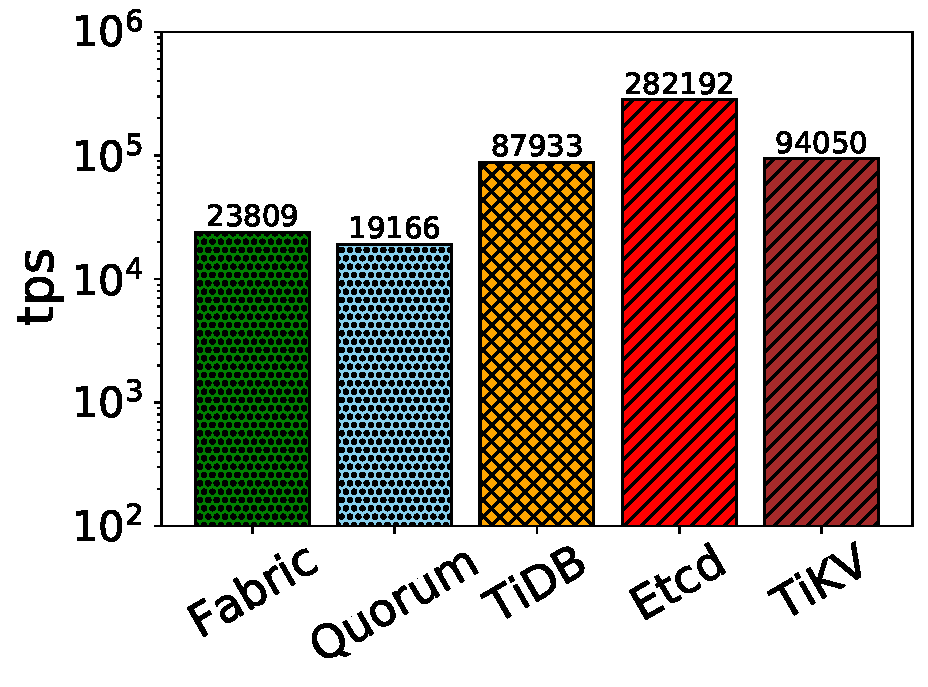
\includegraphics[width=0.99\textwidth]{chart/twin/ycsb-query.pdf}        
        \caption{Query}
    \end{subfigure}
    \caption{Throughput of YCSB workload (log scale).}
    \label{chart:twin:ycsb-thruput}
\end{figure}

\begin{figure}[tp]
	\centering
	\begin{subfigure}{0.45\textwidth}
		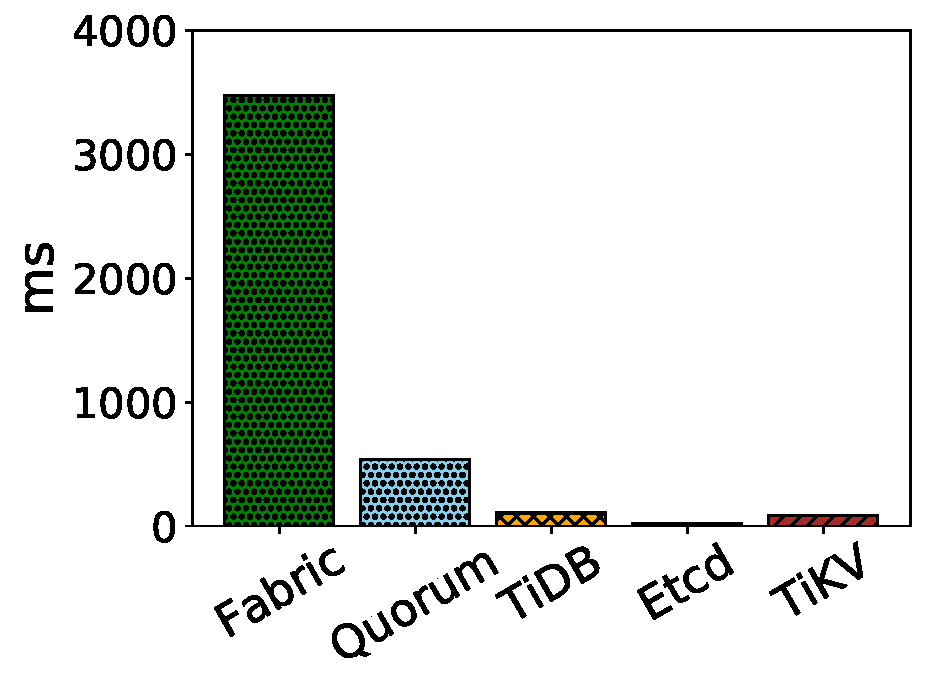
\includegraphics[width=0.99\textwidth]{chart/twin/ycsb-update-delay.pdf}
        \caption{Update}
	\end{subfigure}
	\begin{subfigure}{0.45\textwidth}
		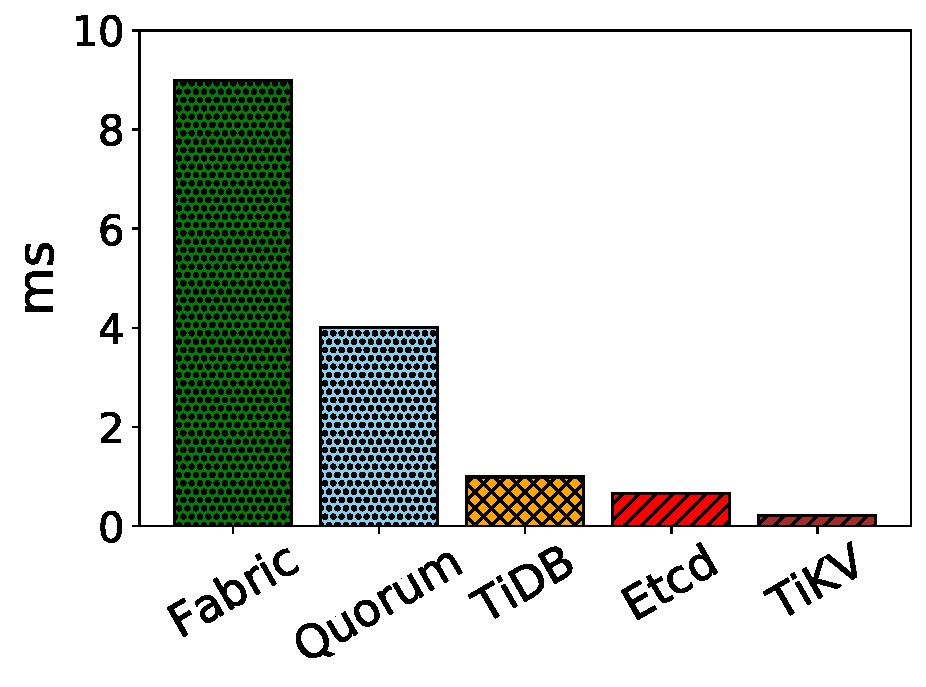
\includegraphics[width=0.99\textwidth]{chart/twin/ycsb-query-delay.pdf}		
        \caption{Query}
	\end{subfigure}
	\caption{Latency of YCSB workload.}
	\label{chart:twin:ycsb-delay}
\end{figure}

We first analyze the peak performance of the four systems under the default
configurations shown in Table~\ref{tab:twin:parameter}.
Specifically, we populate each system with 100K records, each of size $1$ KB.
We then measure the throughput and latency against two YCSB workloads: uniform
update-only (100\% writes) and uniform query-only (100\% reads). We also measure
independently the performance of TiKV, the replicated storage of TiDB, and
include it in this comparison.

Figure~\ref{chart:twin:ycsb-thruput} shows the peak throughput of the five systems.
The relational NewSQL database (TiDB) outperforms the blockchains, while the
replicated storages (etcd and TiKV) outperform the relational database.
Specifically, the two blockchains achieve update throughputs of below $1500$
transactions per second (tps), whereas TiDB achieves $5159$ tps.
The two key-value storages, etcd and TiKV, achieve around $15,000$ tps.
Both outperform the NewSQL database because they do not incur the overhead of
supporting ACID transactions.
This is evidenced by the gap between TiDB and TiKV, caused by the overhead of
the TiDB-server that wraps around the key-value storage.
But this gap is less evident under the query workload, as ACID semantics impose
less constraints on read-only transactions.

Figure~\ref{chart:twin:ycsb-delay} shows the latency when the systems are unsaturated.
Similar to throughput, we observe a clear separation between the blockchains and
the databases.
We note that the blockchains have weaker guarantees for read-only transactions
compared to those offered by the databases (linearizability).
Responses to read requests in the former still take longer (up to $6\times$ in
Fabric) than the linearizable reads in the latter.
The update (query) latency in Fabric and Quorum is around $3500$ms ($9$ms) and
$500$ms ($4$ms) respectively, while in databases it is below $100$ms ($1$ms).

Our results confirm the conclusion drawn in~\cite{dinh2017blockbench} that the
performance of blockchains lags far behind state-of-the-art databases.
However, we observe a smaller gap than that reported
in~\cite{dinh2017blockbench}.
In particular, the relational database, TiDB, achieves $4\times$ greater
throughput than the fastest blockchain, Fabric, under the uniform update
workload (5159 vs.
1294 tps).
This is in contrast with~\cite{dinh2017blockbench}, where H-Store exhibits more
than $120\times$ speedup over blockchains.
The key reason is that H-Store is an in-memory, distributed database with
primary-backup replication.
H-Store represents an extreme point of the design space that makes it rather
dissimilar to blockchains.
In contrast, all systems considered in our work incur some overheads from the
consensus protocols.

\begin{figure}[tp]
	\begin{minipage}{0.45\textwidth}
		\centering
        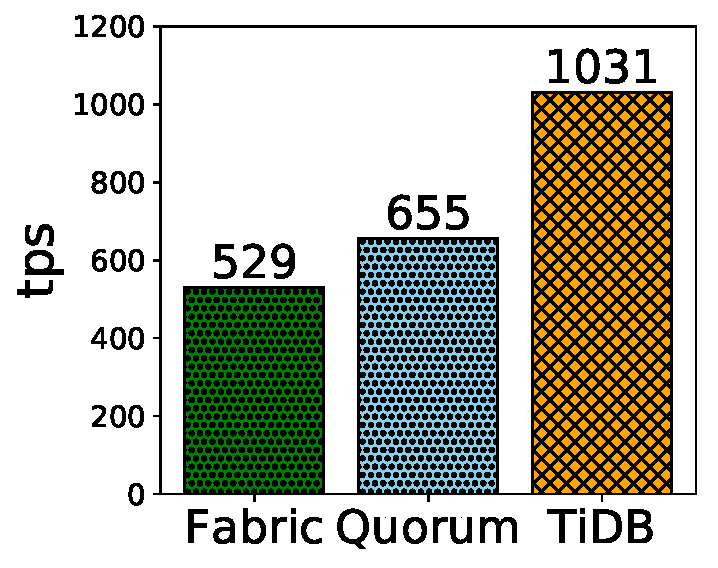
\includegraphics[width=0.99\textwidth]{chart/twin/smallbank.pdf}
		\caption{Throughput of the skewed Smallbank workload (1M records).}
		\label{fig:sb} 
	\end{minipage} \hfill
	\begin{minipage}{0.45\textwidth}
		\centering
		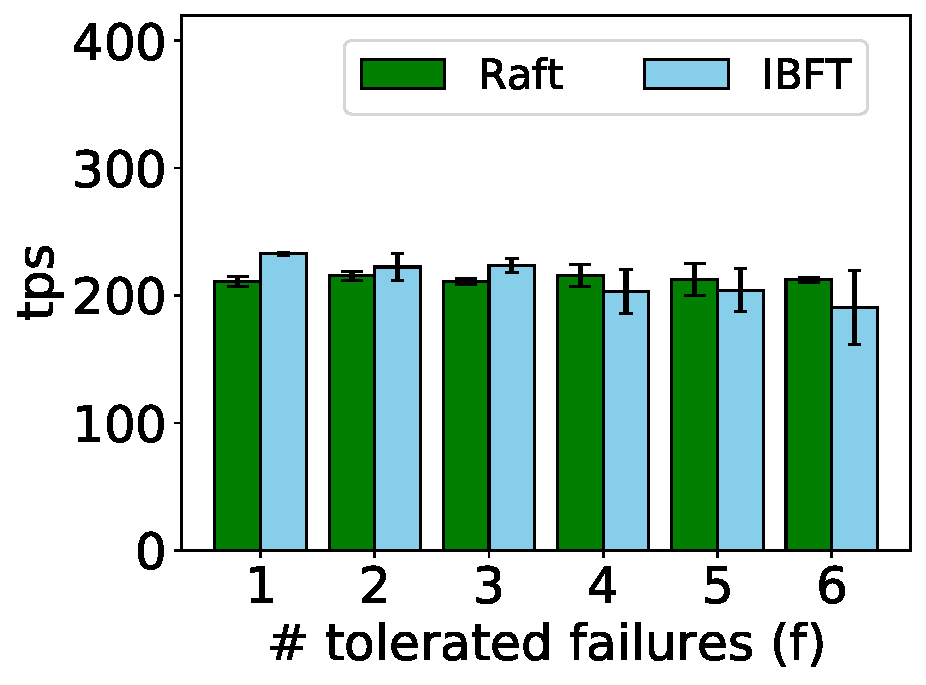
\includegraphics[width=0.99\textwidth]{chart/twin/quorum-consensus.pdf}
		\caption{Quorum throughput with CFT(Raft) and BFT(IBFT).}
		\label{chart:twin:quorum-consensus}
	\end{minipage}
\end{figure}

\subsubsection{Smallbank}

Figure~\ref{fig:sb} compares the OLTP performance under the Smallbank workload.
The request key follows a Zipfian distribution with coefficient $\theta=1$ on 1M
records.
We do not include etcd because it does not support general transactional
workloads.
Compared to YCSB, besides skewness, a Smallbank transaction imposes more
constraints and may touch up to two records, but the record size is smaller.
% For example, sufficient funds must be available for the payment transactions
% to succeed
To our astonishment, the experiments show that the performance difference
between blockchains and distributed databases is small. For example, Faric and
Quorum exhibit throughputs of $835$ and $655$ tps, respectively, while TiDB
exhibits only $1031$ tps.
The performance of Fabric and TiDB drops when switching from YCSB to Smallbank,
while the performance of Quorum improves with a peak throughput under Smallbank
that is $2.5\times$ greater compared to YCSB.
We attribute this improvement to the smaller record size of Smallbank.
As we shall see in Chapter~\ref{sec:twin:exp:txn:record_size}, Quorum's performance
is vulnerable to transactions that access large records.
Likewise, the request skewness accounts for the throughput drop reported by Fabric and TiDB. 

\begin{figure}[tp]
	\centering
	\begin{subfigure}{0.49\textwidth}
		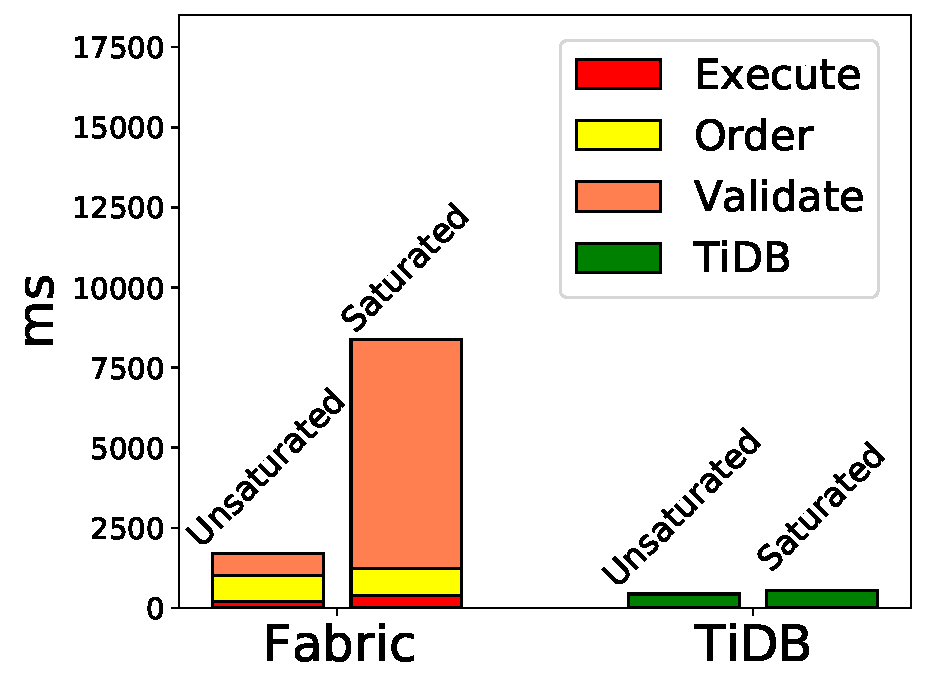
\includegraphics[width=0.99\textwidth]{chart/twin/update-breakdown-v2.pdf}
		\caption{Update}
		\label{chart:twin:update-breakdown}
	\end{subfigure}
	\begin{subfigure}{0.49\textwidth}
		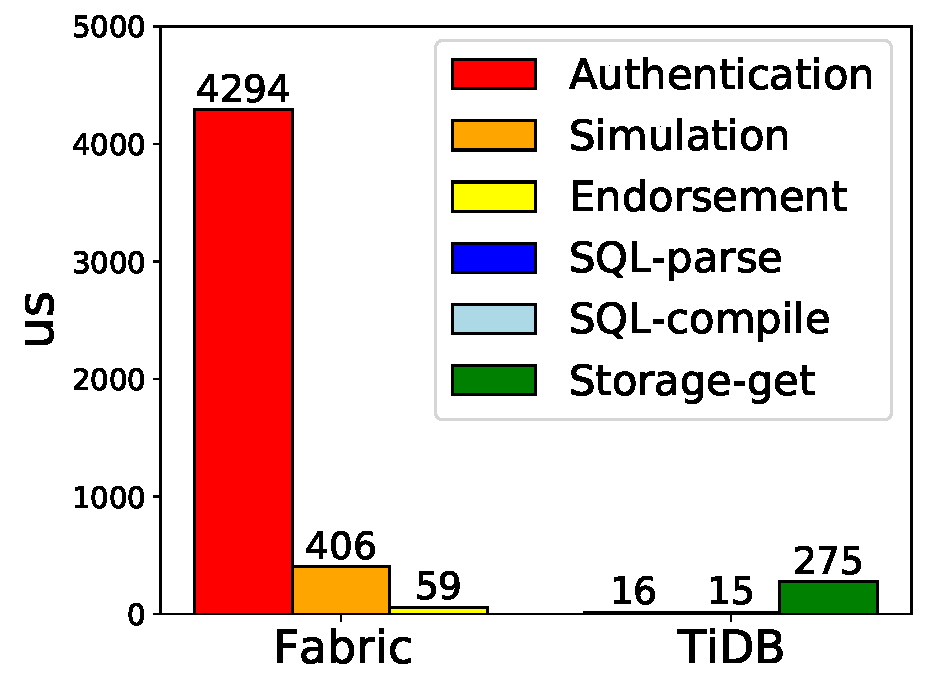
\includegraphics[width=0.99\textwidth]{chart/twin/query-breakdown.pdf}
		\caption{Query}							
		\label{chart:twin:query-breakdown}		
	\end{subfigure}
	\caption{Latency breakdown.}
\end{figure}

\subsection{Replication}

In this experiment, the workload updates only distinct records. 
By reducing the effects of concurrency, we focus on the implications of replication. 

\subsubsection{Effect of replication model}
\label{sec:twin:exp:replication:model}
To understand the impact of the replication model, we focus on Fabric and TiDB
because they support different transaction lifecycles.
Figure~\ref{chart:twin:update-breakdown} compares the latency of a transaction when the
systems are both unsaturated and saturated. Besides its higher latency compared
to TiDB, Fabric exhibits a significant increase in latency when the system is
saturated. To investigate this issue, we instrument Fabric codebase to record
detailed latency breakdown at each phase of a transaction. In particular, we
measure the latency of the execute, order, and validate phases.
When Fabric is unsaturated, the order and validate phases take roughly $700$ms
each, while the execute phase takes below $500$ms.
But when the request rate exceeds the system capacity, validation phase
becomes the bottleneck, as shown in Figure~\ref{chart:twin:update-breakdown}.

We attribute this increase in latency to the serial validation of
blocks in Fabric, where blocks pile up before committing their transactions.
Even inside a block, transactions persist their effects sequentially
based on their internal order.
Worst still, substantial overhead in transaction processing is attributed to
factors other than data processing.
For example, we observe that Fabric, under the saturated scenario, spends $42\%$
of the block validation time to verify the transaction signature.
We note that serial validation is Fabric's implementation choice, i.e., it could
commit transactions concurrently.
However, most of the blockchains impose a strict transaction order to achieve
deterministic execution for security reasons.
In contrast, database transactions do not suffer from such strict sequentiality
under their storage-based replication, nor do they incur security overhead.

The security overhead is the most prominent in query transactions,
which involve no consensus in both systems.
We show in Figure~\ref{chart:twin:query-breakdown} that Fabric spends most of the query
time to authenticate the clients.
In contrast, TiDB incurs no cryptographic overhead and most of its query time is
spent on getting the data.


\subsubsection{Effect of replication approach}
\label{sec:twin:exp:replication:approach}

\begin{table}[tp]
    \centering
    \caption{Throughput (in tps) with varying number of nodes under full replication.}
    \begin{tabular}{@{}lrrrrr@{}}
    \toprule
    \textbf{} & \textbf{3} & \textbf{7} & \textbf{11} & \textbf{15} & \textbf{19} \\ \midrule
    Fabric             & 1560        & 1288        & 1031         & 749         & 528         \\
    % Fabric(solo)       & 1484        & 1207        & 1015         & 729         & 400         \\
    Quorum             & 237        & 236        & 229         & 217         & 219         \\
    TiDB               & 5726       & 8301       & 8898        & 6235        & 5465        \\
    Etcd               & 16492      & 16849      & 9123        & 7801        & 6076        \\ 
	TiKV               & 10369       & 7765       & 7236        & 5516        & 5195        \\
	\bottomrule
    \end{tabular}
    \label{tab:twin:scale}
\end{table}

We increase the number of nodes to compare the scalability of shared log and
consensus-based systems under the full replication mode, and summarize the
results in Table~\ref{tab:twin:scale}.
Here, Fabric is the only shared log system.
Even though Fabric employs the Raft consensus to obtain the transaction order,
this is an external service with 3 fixed orderers. 
The increasing number of Fabric peers consume the same shared ordered log while for the other systems, all their nodes participate in the consensus.

Contrary to our expectations on the two blockchains, we observe neither a constant performance of the
shared log system nor performance degradation in the consensus-based system.
In particular, Fabric's throughput drops $3\times$ from 3 to 19 nodes, while
Quorum's throughput is roughly unchanged.
In Fabric, we find a $38\%$ increase in the block validation latency.
This is because the endorsement policy requires a transaction to be endorsed by
all the nodes.
Hence, more nodes lead to transactions with more signatures and, therefore,
longer validation.
Due to the sequentiality in transaction-based replication, this increase in
validation time translates to the decrease in throughput, as we explained in
Chapter~\ref{sec:twin:exp:replication:model}.
On the other hand, Quorum underutilizes Raft, making its performance insensitive
to the consensus group size.
Specifically, Quorum first pre-executes transactions at the tip of the ledger,
before batching these transactions into a block for the consensus.
Thus, the block proposal rate is affected by the ledger's sequentiality.

Under the same Raft protocol, both NoSQL databases (etcd and TiKV) achieve
higher peak performance compared to the blockchains, but the performance
degrades with the number of nodes.
We attribute this to the consensus protocol.
The NewSQL database does not exhibit either a constant or decreasing performance
trend.
Instead, TiDB reaches its peak performance on 11 nodes.
This is because of the interplay between the consensus overhead in TiKV and the
transaction processing on TiDB servers.
Finally, we conclude that the transaction-based replication model has an obvious
impact on the performance of blockchains, while replication approaches have plain
effects on the performance of distributed databases.

\subsubsection{Effect of failure model}
\label{sec:twin:exp:replication:consensus}
We compare the performance of Raft and Istanbul Byzantine Fault Tolerant (IBFT)
consensus in Quorum to illustrate the impact of different failure models.
Recall that Raft tolerates only crash failures, whereas IBFT can tolerate
Byzantine failures.
IBFT shares the crux of PBFT, which consists of a three-phase commit.
But IBFT is heavily optimized for blockchains.
For example, by embedding the consensus meta-data in the ledger, IBFT saves PBFT
checkpointing efforts.
IBFT additionally accommodates dynamic validators, while PBFT assumes fixed
membership.

% IBFT's distinction from PBFT can be found at Sec 1.2 at
% https://arxiv.org/pdf/1901.07160.pdf.

Figure~\ref{chart:twin:quorum-consensus} shows similar peak throughputs that remain
relatively constant when increasing the number of tolerated failures.
However, we observe that IBFT's throughput exhibits higher variance in larger
networks, as evidenced by the greater error bar. This is due to the larger
quorums needed in IBFT, which are $2f+1$ out of $3f+1$, compared to $f+1$ out of
$2f+1$ replicas needed in Raft.
IBFT needs to contact more replicas in a time window compared to Raft to avoid
the view change, during which the corresponding transaction processing is
interrupted.
When $f$ increases, the probability of such interruption increases accordingly,
hence, this leads to larger variances in performance.

\subsection{Concurrency} 
\label{sec:twin:exp:concurrency}
In the following experiments, we twist the workload to understand the effects of
concurrency on system performance.
To reduce the effects of replication, the number of nodes is fixed to 5 and full
replication is used.

\subsubsection{Effect of skewness}

\begin{figure}[tp]
	\centering
	\begin{subfigure}{0.45\textwidth}
		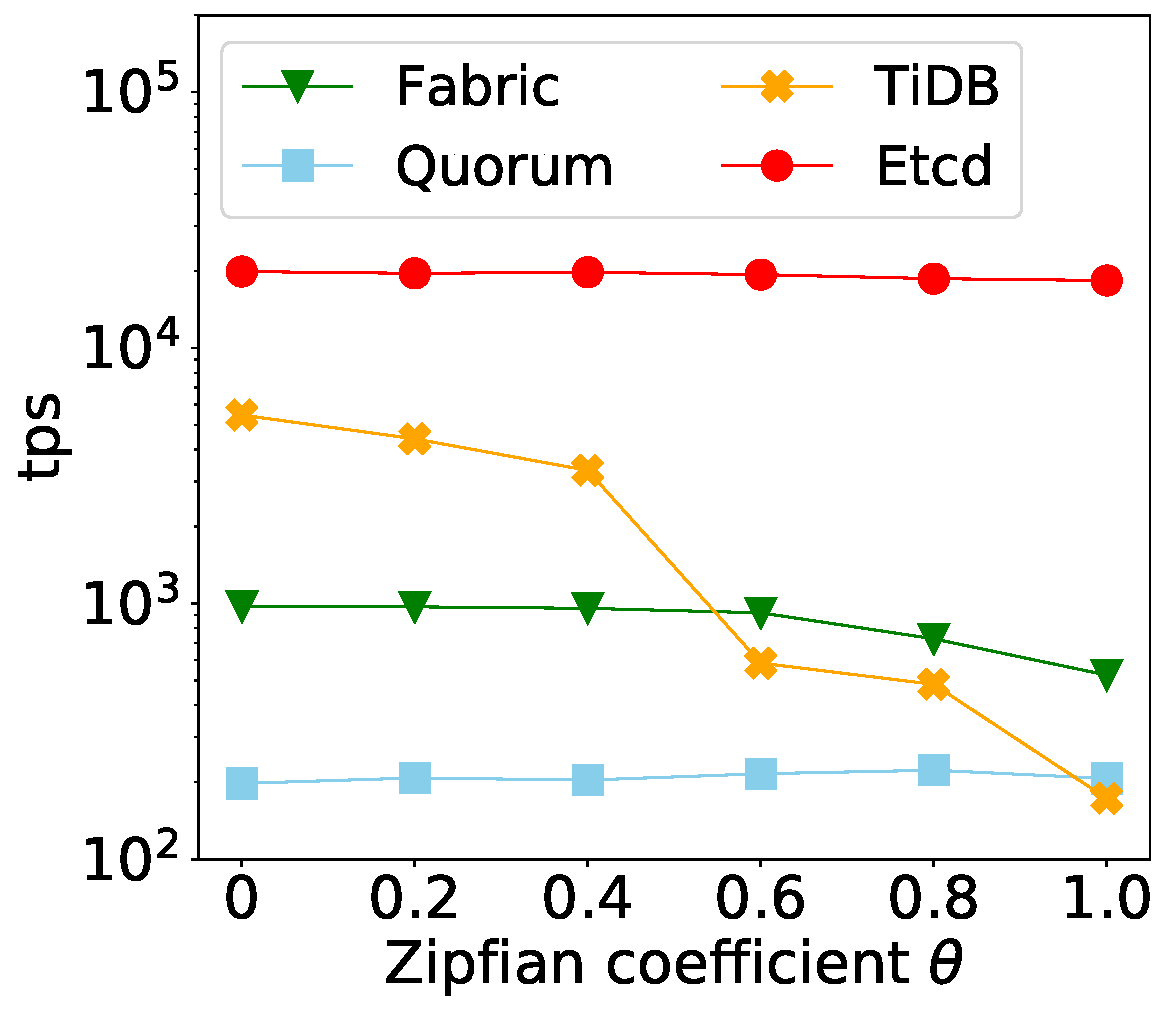
\includegraphics[width=0.99\textwidth]{chart/twin/skew.pdf}
		\caption{Throughput (log scale)}        
		\label{chart:twin:skew-thruput}
	\end{subfigure}
	\begin{subfigure}{0.45\textwidth}
		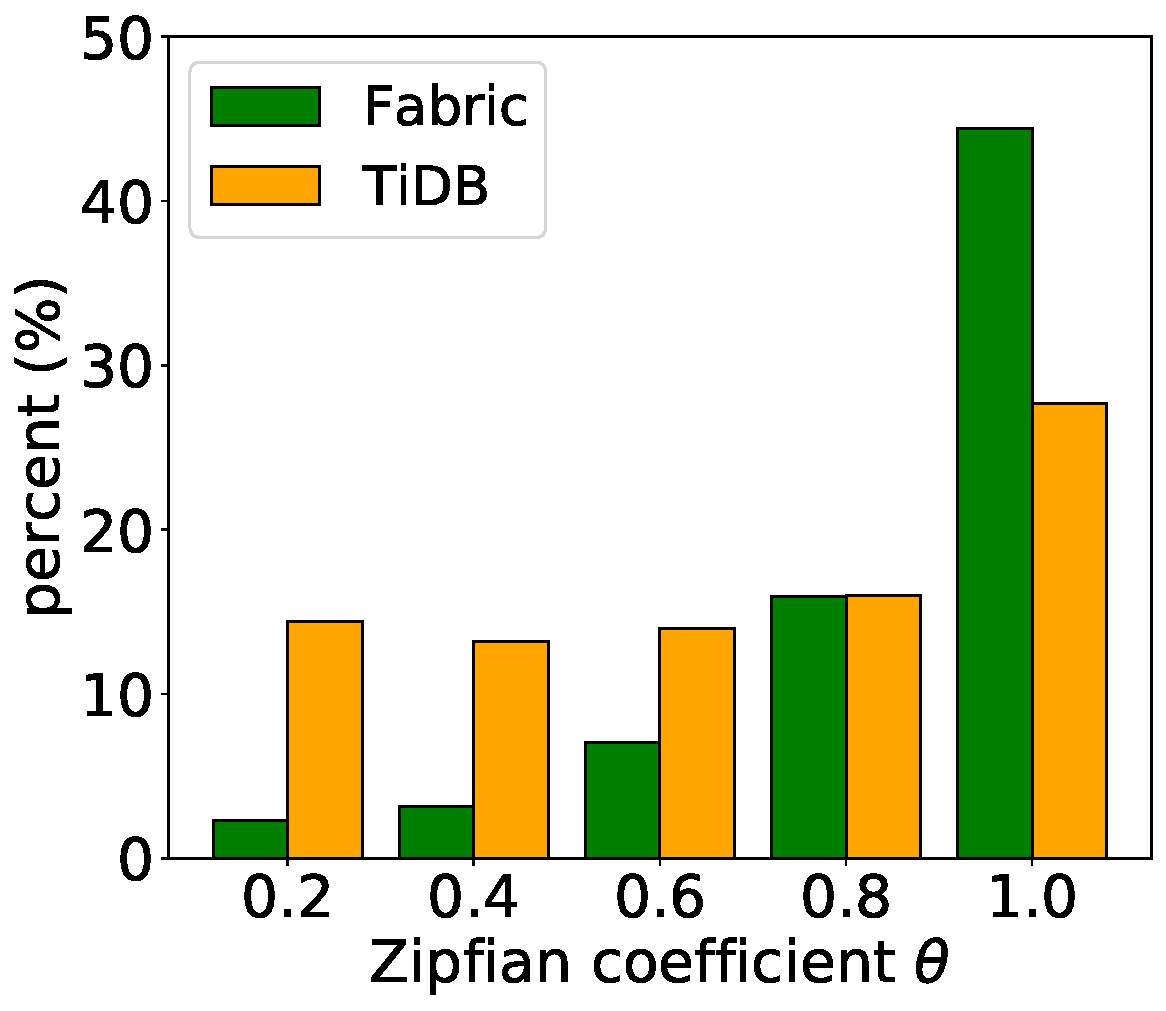
\includegraphics[width=0.99\textwidth]{chart/twin/skew-abort.pdf}
		\caption{Abort rate}        
		\label{chart:twin:skew-abort}
	\end{subfigure}
	\caption{Throughput and abort rate with skewed workloads. Each transaction modifies a single record.}
	\label{chart:twin:skew}
\end{figure}

To analyze the effect of concurrency control mechanisms, we use skewed workloads
in which each transaction modifies (first read, then update and write back) a
single record.
The records' keys follow a Zipfian distribution that varies based on the
skewness coefficient $\theta$.
Figure~\ref{chart:twin:skew} shows the throughputs and the corresponding abort rates
under different skewness.
Our key observation here is that blockchains and databases are comparable under
a high contention workload, given the fact that TiDB drastically drops from
$5461$ to $173$ tps when $\theta$ increases from $0$ to $1$.
Etcd and Quorum do not have concurrency control because they execute
transactions serially. Thus, their performance is not affected by skewness.

Although Fabric commits transactions sequentially, we observe a $31\%$ drop in
throughput from a uniform to a skewed workload with $\theta=1$.
This is due to Fabric's optimistic concurrency control on read-write conflicts.
That is, a transaction contains the versions of the records read during the
proposal phase, which are then checked in the validation phase.
If the versions are not the latest, the transaction aborts.
A skewed workload means that many transactions are accessing the same records,
leading to a higher probability of transaction abort.
For example, Figure~\ref{chart:twin:skew-abort} shows that $44\%$ of the transactions
in Fabric abort when $\theta=1$.

Another interesting observation is that TiDB's throughput drop is
disproportional to its increase in abort rate.
Specifically, when $\theta=1$, only $30\%$ of TiDB's transactions fail but the
throughput decreases by $90\%$.
This is because each transaction coordinator must obtain a latch on a primary
record, whose write outcome determines the overall transaction status.
But write must undergo the consensus for replication.
Under a highly skewed workload, such a latching mechanism makes the transaction
coordinator spend more time on contention resolution than the actual execution
of the transaction payload, resulting in a remarkable decrement of the overall
throughput.
Hence we conclude that the workload skewness exerts a tremendous impact on
storage-based replicated, concurrency-over-replication architectures.

\subsubsection{Effect of operation count}

\begin{figure}[tp]
	\centering
	\begin{subfigure}{0.45\textwidth}
		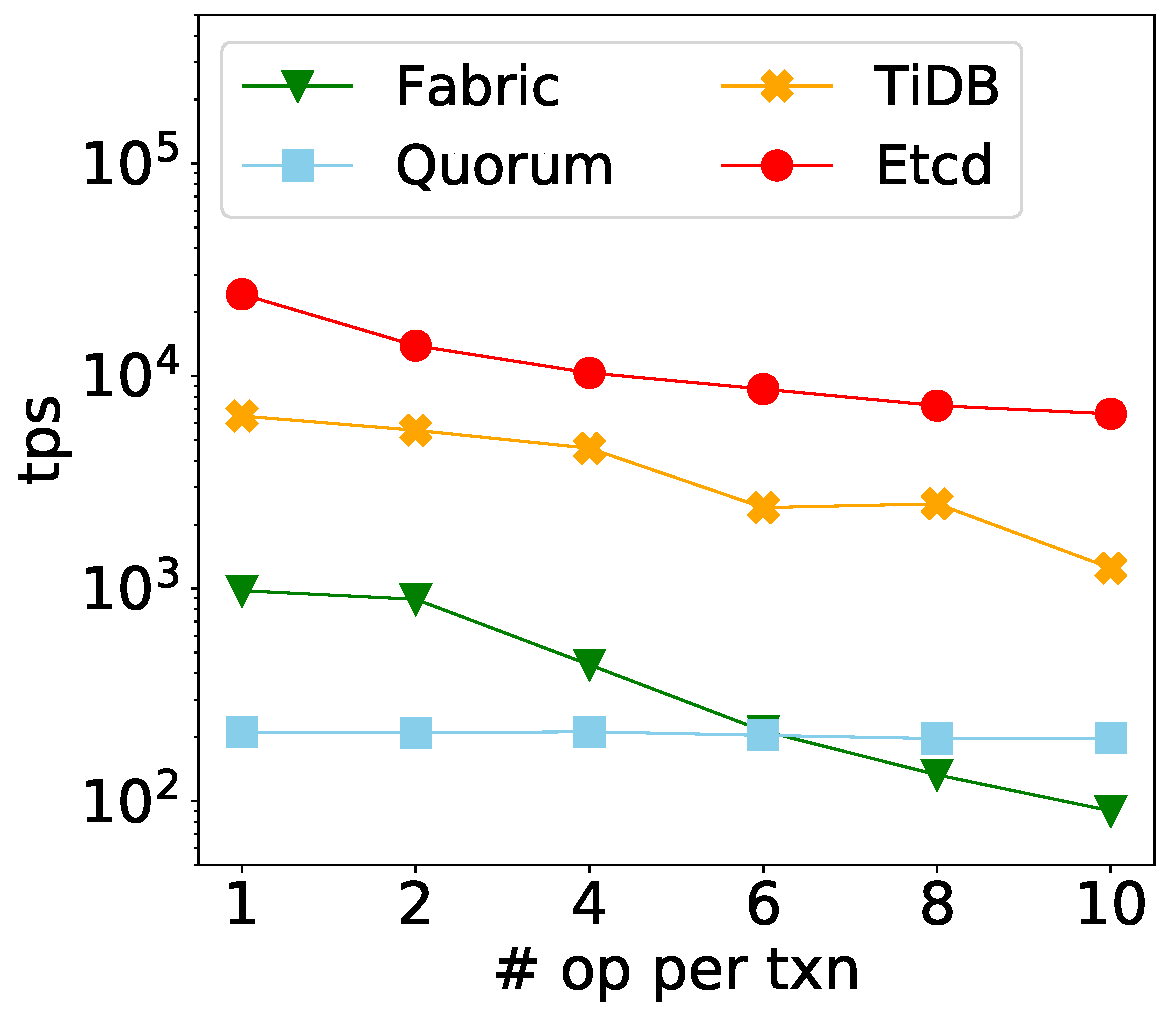
\includegraphics[width=0.99\textwidth]{chart/twin/txn-size.pdf}
		\caption{Throughput (log scale)}        
		\label{chart:twin:txn-size}
	\end{subfigure}
	\begin{subfigure}{0.45\textwidth}
		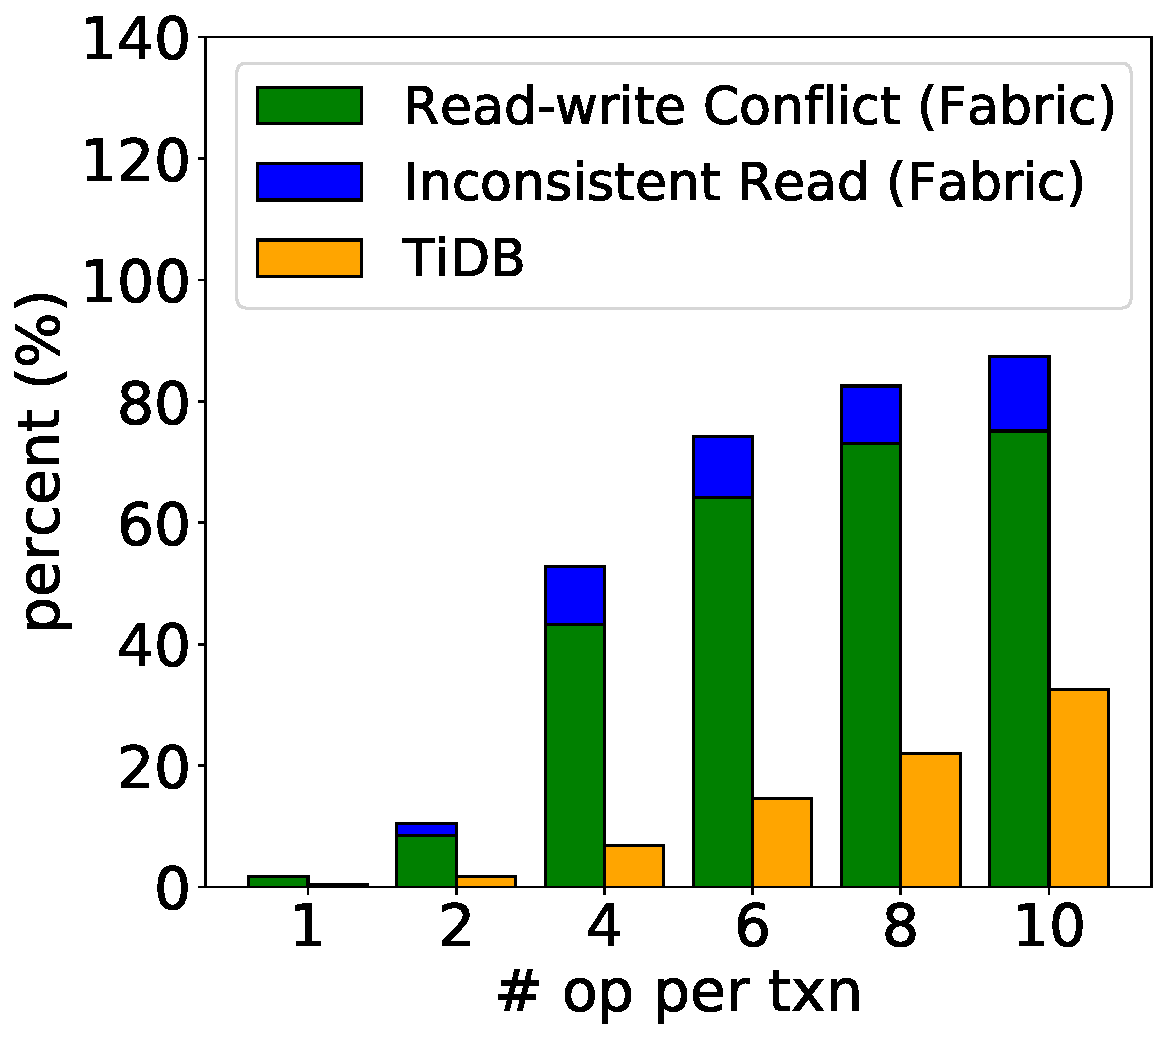
\includegraphics[width=0.99\textwidth]{chart/twin/txn-size-abort.pdf}
        \caption{Abort rate}
		\label{chart:twin:txn-size-abort}
	\end{subfigure}
	\caption{Throughput and abort rate with uniformly modified records in a single
	transaction.}
	\label{chart:twin:txn-size-fig}
\end{figure}

We gradually include more update operations per transaction to analyze the
impact of transaction atomicity on performance. 
To remove the effect of transaction size, for a given number of operations we
vary the record size such that the total transaction size is $1000$ bytes. 
For example, if a transaction writes 10 records, then each record contains
100 bytes.

As shown in Figure~\ref{chart:twin:txn-size}, the performance of Fabric, TiDB, and etcd
drops when the number of operations per transaction increases.
In particular, with 10 operations per transaction, TiDB achieves only $32\%$ of
the throughput of single operation transactions.
Two sources of overheads contribute to this drop in performance.
First, there are more conflicts when a transaction writes to more records, which
leads to a higher abort rate.
Second, TiDB uses sharding, which means that a 10-operation transaction may span
multiple shards.
As there are more shards, the overhead of the 2PC coordination in TiDB
increases.
Etcd and Quorum are unaffected because they do not entail cross-shard
transactions.

Figure~\ref{chart:twin:txn-size-abort} shows the abort rate of TiDB and Fabric as the
number of operations per transaction increases.
Both systems experience high abort rates: $26.9\%$ for TiDB and $87\%$ for
Fabric.
Interestingly, while TiDB aborts are mostly due to write-write conflicts, aborts
in Fabric come from two sources: inconsistent reads and the read-write
conflicts.
On the one hand, during the proposal phase in Fabric, a client must collect
identical read results from the peers.
This is because we mandate that each transaction proposal must be simulated and
endorsed by all peers.
But different results may be returned, as the peers have disjoint states, which
is highly likely since they commit blocks at different rates.
In this case, the client immediately aborts the transaction.
On the other hand, any of the modified records exhibiting a read-write conflict
may render the transaction invalid.
Under 10 operations per transaction, these two sources take up $14\%$ and $86\%$
of all the aborts, respectively.

\subsubsection{Effect of record size}
\label{sec:twin:exp:txn:record_size}

\begin{figure}[tp]
	\centering
	\begin{subfigure}{0.45\textwidth}
		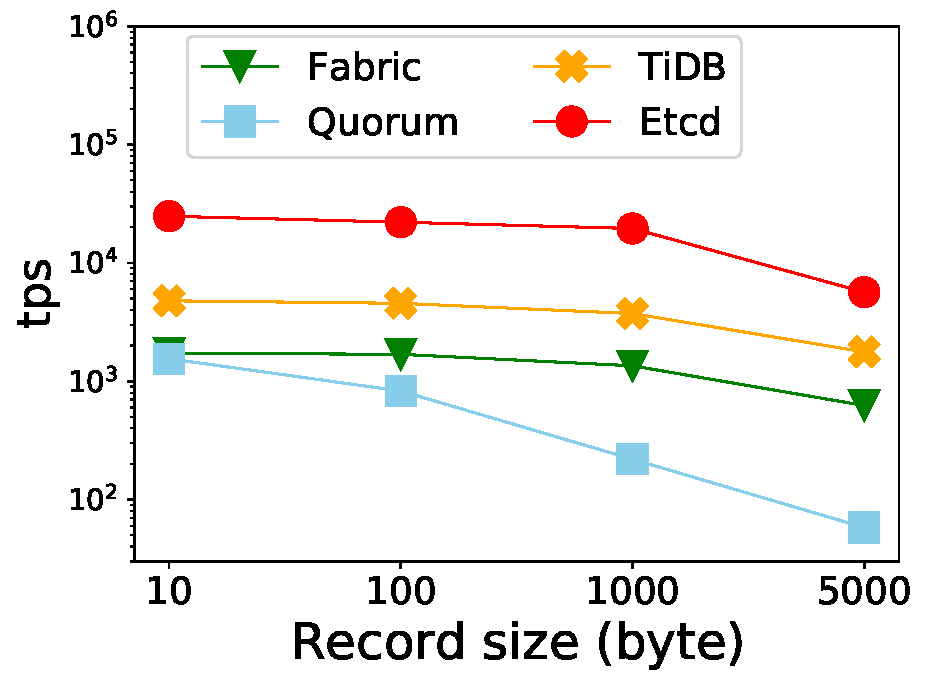
\includegraphics[width=0.99\textwidth]{chart/twin/record-size-thruput.pdf}        
		\caption{Throughput}
		\label{chart:twin:record-size-thruput}
	\end{subfigure}
	\begin{subfigure}{0.45\textwidth}
		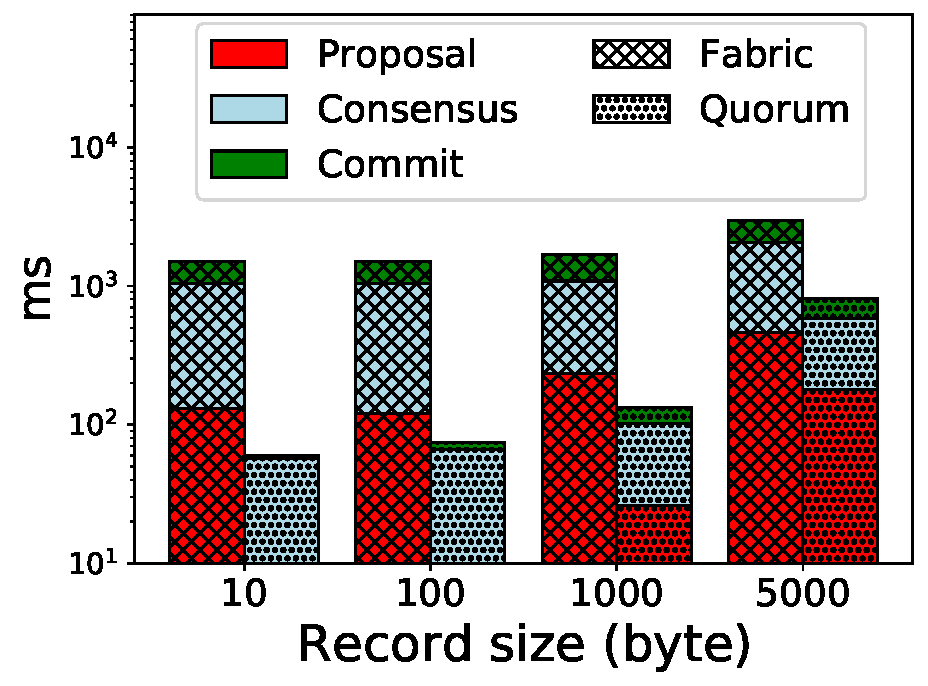
\includegraphics[width=0.99\textwidth]{chart/twin/record-size-breakdown.pdf}     
		\caption{Latency breakdown}
		\label{chart:twin:record-size-breakdown}
	\end{subfigure}
	\caption{Performance under uniform update workload with increasing record size.
	Both plots use log scale.}
\end{figure}

We enlarge the record in the uniform-update workload to increase the complexity
per transaction without aggravating the inter-transaction conflicts.
As shown in Figure~\ref{chart:twin:record-size-thruput}, all the databases exhibit
moderate throughput decrease and latency increase.
However, the two blockchains behave differently.
When the record grows from $10$ to $1,000$ bytes, Fabric's performance remains
roughly constant at 1400 tps and drops by half on $5,000$ bytes.
But Quorum suffers a significant drop in throughput, from $1547$ tps on
$10$-byte to $58$ tps on $5000$-byte records.
To understand this, we analyze the transaction latency breakdown in Fabric and
Quorum, and present the results in Figure~\ref{chart:twin:record-size-breakdown}.
The block commit time in Fabric only doubles, whereas in Quorum there is a
$70\times$ increase from $3$ms for $10$-byte records to $221$ms for $5000$-byte
records, reducing the proportion of the consensus from $88\%$ to $50\%$ in a
transaction lifecycle.
For each commit, Quorum's virtual machine needs to reconstruct an MPT data
structure, which involves many expensive cryptographic hash computations.
At the same time, the cost of a hash function increases with the record size.
In particular, we find that the cost of MPT reconstruction increases from $56$us
to $2.5$ms when the record size grows from $10$ to $5000$ bytes.

Another interesting observation from Figure~\ref{chart:twin:record-size-breakdown} is
that the delay of the proposal phase in Quorum grows at the same rate as the
delay of the commit phase.
This is due to Quorum's order-execute model, where transactions are firstly
batched and serially executed during the proposal phase by the proposer.
After consensus, the batched transactions are serially executed again by all the
other nodes for validation and commit.
Hence, Quorum's performance suffers from both double execution and the overhead
of sequential validation of in-block transactions.
In contrast, Fabric adopts an execute-order-commit model where transactions are
executed concurrently during the proposal phase, before being ordered and
batched in the consensus phase. 
The serial processing only occurs once during the commit phase. 
However, concurrency comes at the cost of potentially aborted in-block
transactions that would break the serializability, as we saw in the previous
section.
Hence, when the transactions are computationally heavy, execute-order-commit
blockchains outperform order-execute blockchains by introducing the
sequentiality requirement later.
But compared with blockchains, NewSQL databases with storage-based replication
can harness more concurrency.

\subsection{Storage}
In this section, we analyze the storage overhead for the ledger abstraction and
the authenticated data structures.

\begin{figure}[tp]
	\begin{minipage}{0.45\textwidth}
		\centering
		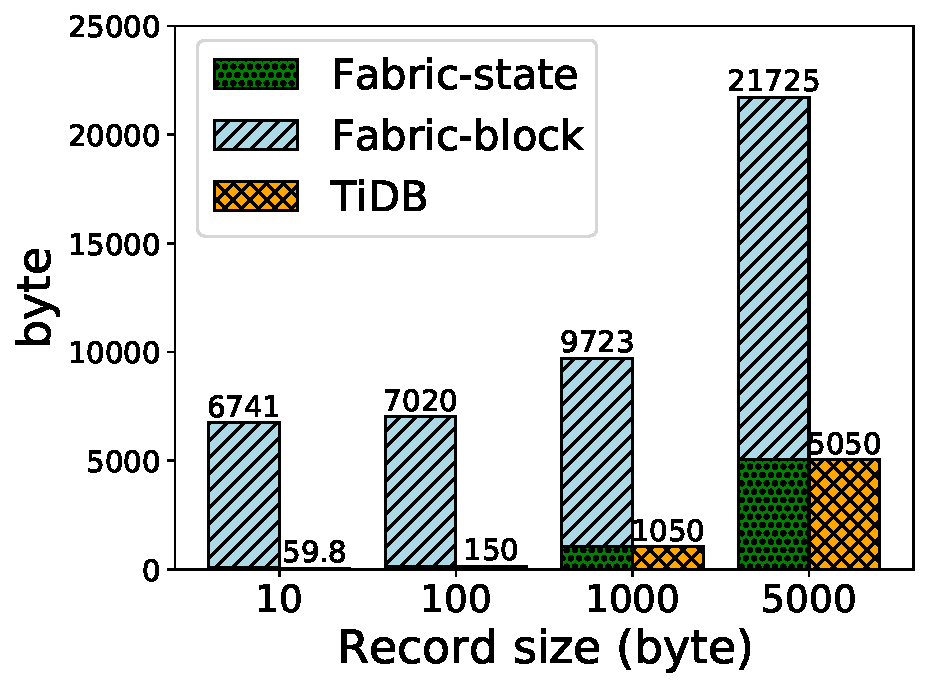
\includegraphics[width=0.99\textwidth]{chart/twin/record-size-storage.pdf}
		\caption{Storage breakdown \\ in Fabric and TiDB.}
		\label{chart:twin:record-size-storage}
	\end{minipage}\hfill
	\begin{minipage}{0.45\textwidth}
		\centering
		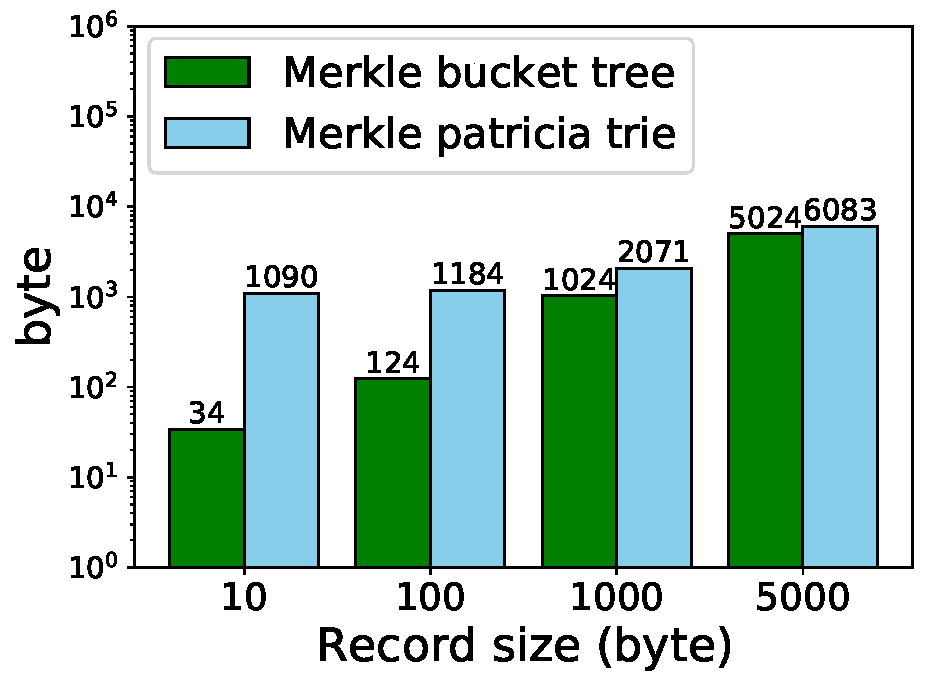
\includegraphics[width=0.99\textwidth]{chart/twin/record-size-antitamper.pdf}
		\caption{Storage overhead to achieve tamper evidence (log scale).}
		\label{chart:twin:record-size-antitamper}
	\end{minipage}\hfill
 \end{figure}

 \subsubsection{Effect of record size on storage}

Figure~\ref{chart:twin:record-size-storage} shows the storage cost per record as we
increase the record size.
Fabric incurs a much higher storage overhead than TiDB.
For a $5000$-byte record, the state storage consumes around $5000$ bytes, while
the block storage consumes $21,725$ bytes.
There is no additional storage used by TiDB because no historical information is
maintained and the associated metadata is negligible.
This result demonstrates that blockchains incur significantly higher storage
costs than databases because of the underlying ledger abstraction.

\subsubsection{Security overhead for tamper evidence}
\label{sec:twin:exp:storage:tamper}

To quantify the overhead incurred by the integrity protection mechanism in
blockchains, we compare the performance of Merkle Bucket Tree (MBT) from
Hyperledger Fabric v0.6\footnote{Fabric v1.0 and later relax the security model
and no longer require tamper-evident indexes.} and Merkle Patricia Trie (MPT)
from Quorum.
This comparison is done on the system behavior in its entirety. We
refer readers to~\cite{yue2020analysis} for an in-depth analysis.

For this comparison, we insert 10K records of different sizes and measure the
state storage cost per record. 
Figure~\ref{chart:twin:record-size-antitamper} shows
that MBT adds extra $24$ bytes per record, while MPT adds over 1KB per record.
Since both MBT and MPT store data records in the leaves, their differences come
from the tree structures: the deeper the tree, the higher the storage overhead.
The scale of MBT is fixed.
Specifically, MBT first hashes all the records into $1,000$ buckets, on top of
which a Merkle tree with a given fan-out is built.
Considering $1,000$ buckets and a fan-out of $4$ in our experiments, the depth
of the tree is capped at 5 ($\ceil{log_4 1000}$).
As a prefix tree, the depth of MPT is affected by the key length, which is 16
bytes in our setting.
Specifically, each internal MPT node holds 4 bits of the key, hence, the depth
and fan-out can go up to 32 and 16, respectively.
This explains why MPT needs more space.

\subsection{Sharding}
\label{sec:twin:exp:shard}

\begin{figure}[tp]

	\centering
	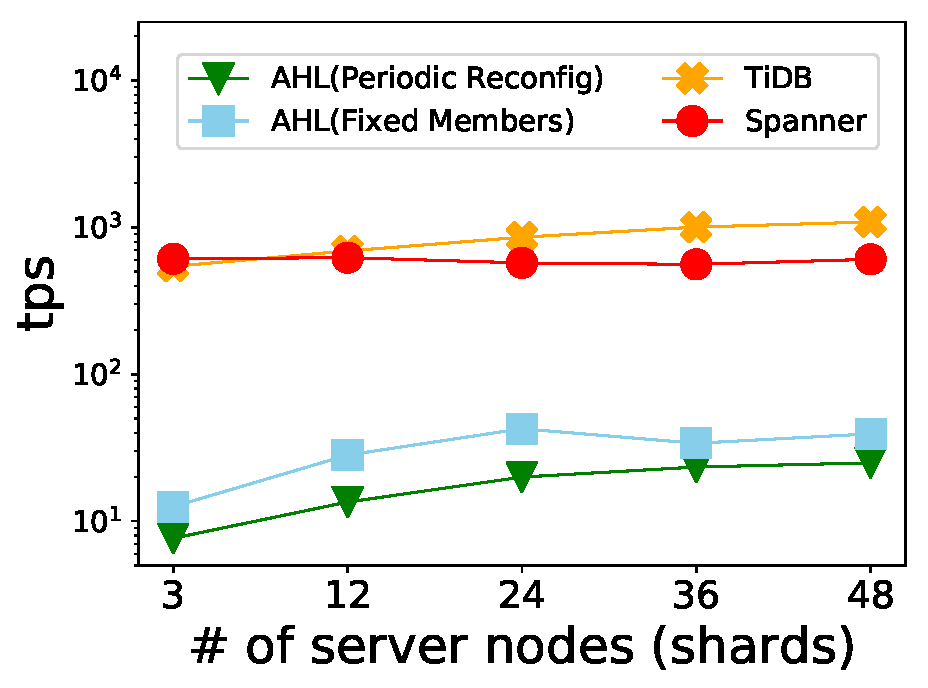
\includegraphics[width=0.6\textwidth]{chart/twin/skewed-scale.pdf}
	\caption{Throughput of the skewed workload (log scale).}
	\label{chart:twin:shard}
\end{figure}

To compare the impact of sharding on databases and blockchains, we disable full
replication in TiDB, and compare its performance with Spanner, a cloud-based
NewSQL database, and Attested Hyperledger (AHL)~\cite{dang2018towards}, a
state-of-the-art sharded blockchain based on Hyperledger Fabric v0.6.
AHL leverages trusted hardware to reduce shard size and to improve throughput
per shard.
It supports cross-shard transactions by running a BFT shard that implements a
2PC state machine, and periodically reconfigures shards to mitigate adaptive
adversaries.
This experiment is run on Google Cloud Platform since Spanner is a cloud-only
service.
We set the number of nodes in a shard to 3 for all the systems, and we
pre-populate the state with 1M 1KB-size records.
We evaluate the systems with a skewed workload with a Zipfian coefficient of
$\theta=1$, in which each transaction modifies two records.

Figure~\ref{chart:twin:shard} shows that TiDB achieves higher throughput compared to
Spanner when increasing the number of nodes (and shards).
This is because TiDB instantly aborts a transaction once detecting a conflict.
In contrast, conflicting transactions in Spanner would contend for locks under
the pessimistic concurrency control.
To achieve stronger security, AHL with periodic shard re-configuration trades
off $30\%$ in performance compared to AHL with fixed shards.
Nonetheless, the gap between AHL and both the databases is large, due to the
high cost of PBFT and other security overheads.

\subsection{Performance of Hybrid Systems}
\label{sec:twin:exp:hybrids}
\begin{figure}
	\centering
	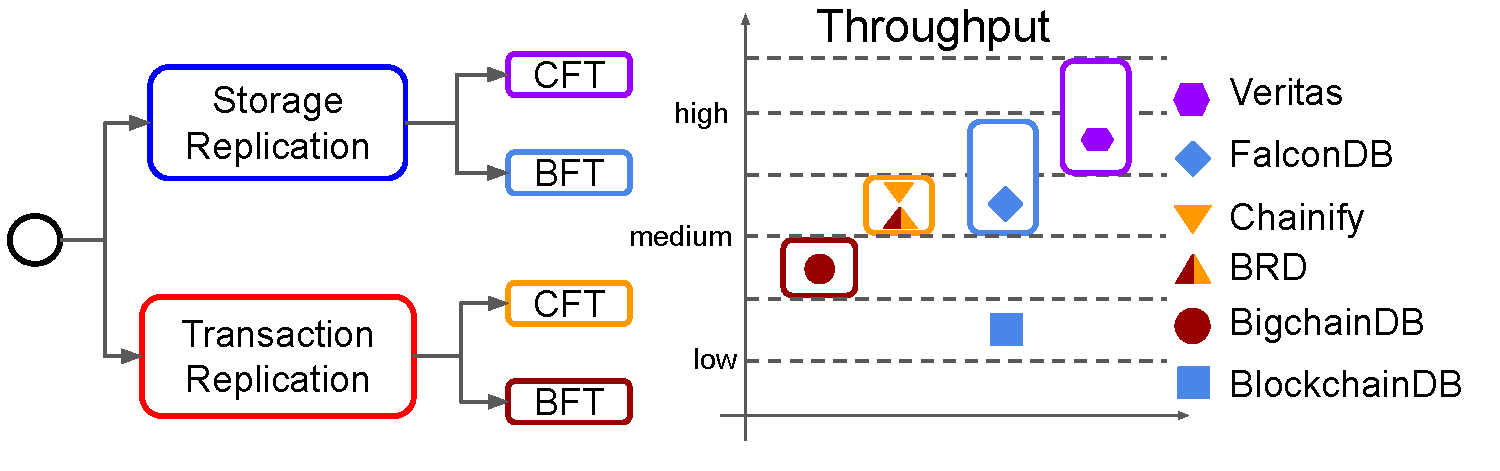
\includegraphics[width=0.8\textwidth]{diagram/twin/performance_framework.pdf}
	\caption{The framework for understanding the throughput of hybrid systems.
	The systems are color-coded based on the design choices.} 
	\label{diagram:twin:perf_framework}
\end{figure}

Based on our taxonomy and experimental results, we propose a framework for
comparing the performance of existing hybrid systems.
We emphasize that the framework only supports high-level, back-of-the-envelope
comparison, and is not a replacement for detailed experimental analysis.
It focuses on throughput as the key performance metric and does not consider all
the dimensions in our taxonomy.
However, this framework explains the performance differences among systems
according to their reported results.
More importantly, it can guide the design of future hybrid systems.

Figure~\ref{diagram:twin:perf_framework} presents our framework together with the
reported performance of some hybrid systems.
We note that the replication model is the deciding factor in determining the
peak throughput.
The results in Chapter~\ref{sec:twin:exp:replication:model} show that the replication
model affects concurrency.
In particular, transaction-based replication exposes lower concurrency than
storage-based replication, which results in lower throughput.
The next factor that affects throughput is the failure model.
As explained in Chapter~\ref{sec:twin:taxonomy:replication:failure}, CFT protocols
are more efficient than BFT protocols due to their lower network overhead,
therefore, systems using CFT are likely to have higher throughput.
This is true especially when the CFT protocol is implemented as a shared log
service.
We note that even though our experiments do not show much difference between CFT
and BFT in Quorum, it is because these protocols are not the bottleneck.

Figure~\ref{diagram:twin:perf_framework} illustrates the reported performance of six
hybrid systems within our framework.
Using the two factors stated above, we can predict the throughput effectively.
For instance, Vertias exhibits better throughput than Chainify ($29k$ vs.
$6.1k$) because it uses storage-based replication and CFT protocols.
But its performance has a high variance because, under high contention, the
throughput can decrease significantly, as explained in
Chapter~\ref{sec:twin:exp:concurrency}.
\chapter{Fine-Grained, Secure and Efficient Data Provenance on Blockchains}
\label{ch:prov}

\section{Introduction}
\label{sec:provenance:intro}
Blockchains are disrupting many industries, including
finance~\cite{tapscott2017blockchain,nguyen2016blockchain}, supply
chain~\cite{korpela2017digital,tian2016agri}, and healthcare~\cite{medilot}. These industries are exploiting
two distinct advantages of blockchains over traditional data management systems. First, a blockchain is
decentralized, which allows mutually distrusting parties to manage the data together instead of trusting a
single party.  Second, the blockchain provides integrity protection (tamper evidence) to all transactions
recorded in the ledger. In other words, the complete transaction history is secure.  

The management of data history, or data provenance, has been extensively studied in databases, and  many
systems have been designed to support
provenance~\cite{cheney2009provenance,chiticariu2005dbnotes,buneman2006provenance,park2011ramp,akoush2013hadoopprov,wang2015big}.
In the context of blockchain, there is explicit, but only coarse-grained support for data provenance. In
particular, the blockchain can be seen as having some states (with known initial values), and every
transaction moves the system to new states.  The evolution history of the states (or provenance) can be
securely and completely reconstructed by replaying all transactions. This reconstruction can be done 
during offline analysis. During contract execution (or runtime), however, no provenance information is
safely available to smart contracts. In other words, smart contracts cannot access historical blockchain
states in a tamper-evident manner. The lack of secure, fine-grained, runtime access to provenance therefore restricts the expressiveness of the business logic the contract can encode.

Consider an example smart contract shown in Figure~\ref{code:prov:contract}, which contains a method for transferring a
number of tokens from one user to another. Suppose user $A$ wants to send tokens to $B$ based on the latter's
historical balance in recent months. For example, $A$ only sends token if $B$'s average balance per day is
more than $t$. It is not currently possible to write a contract method for this operation. To work around
this, $A$ needs to first compute the historical balance of $B$ by querying and replaying all on-chain
transactions, then based on the result issues the \texttt{Transfer} transaction. Besides performance
overhead incurred from multiple interactions with the blockchain, this approach is not {\em safe}: it fails to
achieve transaction serializability. In particular, suppose $A$ issues the \texttt{Transfer} transaction
$tx$ based on its computation of $B$'s historical balance. But before $tx$ is received by the
blockchain, another transaction is committed such that $B$'s average balance becomes $t' < t$. Consequently,
when $tx$ is later committed, it will have been based on stale state, and therefore fails to meet the intended
business logic. In blockchains with native currencies, serializability violation can be exploited for
Transaction-Ordering attacks that cause substantial financial loss to the users~\cite{luu2016making}.

\begin{figure}
    \footnotesize
    \centering
    \begin{verbatim}
    contract Token {
        method Transfer(sender, recipient, amount) {
            bal1 = gState[sender];
            bal2 = gState[recipient];
            if (amount < bal1) {
                gState[sender] = bal1 - amount;
                gState[recipient] = bal2 + amount;
        } 
      } 
    }
    \end{verbatim}
\caption{A smart contract that manages for token management.}
\label{code:prov:contract}
\end{figure}

In this paper, we design and implement a fine-grained, secure and efficient provenance system for blockchains,
called {\fs}. In particular, we aim to enable a new class of smart contracts that can access provenance
information at runtime. Although our goal is similar to that of existing works in adding provenance to
databases~\cite{akoush2013hadoopprov,tian2016agri,psallidas2018smoke}, we face three unique challenges due to
the nature of blockchain. First, there is a lack of data operators whose semantics capture
provenance in the form of input-output dependency. More specifically, for general data management workloads (i.e.,
non-cryptocurrency), current blockchains expose only generic operators, for example, \texttt{put} and \texttt{get}
of key-value tuples. These operators do not have input-output dependency. In contrast, relational databases
operators such as \texttt{map}, \texttt{join}, \texttt{union}, are defined as relations between input and output, which
clearly capture their dependencies. To overcome this lack of provenance-friendly operators, we instrument
blockchain runtime to record read-write dependency of all the states used in any contract invocation, which is
then passed to a user-defined method that specifies which dependency to be persisted. 

The second challenge is that blockchains assume an adversarial environment, therefore any captured provenance
must be made tamper evident. To address this, we store provenance in a Merkle tree data structure
that also allows for efficient verification. The final challenge is to ensure that provenance queries are
fast, because a large execution overhead is undesirable due to the Verifier's
Dilemma~\cite{luu2015demystifying}. To address this challenge, we design a novel skip list index that is optimized
for provenance queries. The index incurs small storage overhead, and its performance is independent of the number of blocks in the blockchain. 

In summary, we make the following contributions: 
\begin{itemize}
  \item We introduce a system, called {\fs} that efficiently captures fine-grained provenance for
  blockchains. It stores provenance securely, and exposes simple access interface to smart contracts. 

  \item We design a novel index optimized for querying blockchain provenance. The index incurs small
  storage overhead, and its performance is independent of the blockchain size. 
  It is adapted from the skip list but we completely remove the randomness to fit for deterministic blockchains. 

  \item We implement {\fs} for Hyperledger Fabric v2.2~\cite{github:fabric}. Our implementation builds on top of
  ForkBase, a blockchain-optimized storage~\cite{wang2018forkbase}. We conduct extensive
  evaluation of {\fs}. The results demonstrate its benefits to provenance-dependent applications, and
  its efficient query and small storage overhead. 
\end{itemize}

The remainder of the chapter is organized as follows. \Cref{sec:provenance:background} provides necessary blockchain preliminaries for the understanding. \Cref{sec:provenance:capture} describes our design for capturing provenance, and the interface
exposed to smart contracts. \Cref{sec:provenance:storage} discusses how we store provenance, and
\Cref{sec:provenance:index} describes our new index. \Cref{sec:provenance:implementation} presents our
implementation. \Cref{sec:provenance:exp} reports the performance of {\fs} on provenance-related matters. 

\section{Preliminary}
\label{sec:provenance:background}
In this section, we present more background on blockchain systems.
We especially focus on the block structure and the procedure to validate a block. 
And we explain the design choices of state organization that affect index structure requirements.
At last, we present an overview of {\fs}. 

\textbf{Data model.} Different blockchains adopt different data models for their states. Bitcoin' states
are unspent coins modeled as Unspent Transaction Outputs (UTXOs), as detailed in \Cref{sec:literature:datamodel}. More recent blockchains, namely Ethereum and Fabric, support general states that can be modified arbitrarily
by smart contracts.  They adopt an account-based data model, in which each account has its own local states
stored on the blockchain. A smart contract transaction can write arbitrary data to the storage. This flexible
data model comes at the cost of integrity protection and verification of the account states. In this paper, we
focus on the account-based data model.

\textbf{Block structure.} A block in the blockchain stores the transactions and the global states.
The block header contains the following fields.  
\begin{itemize} 
    \item \texttt{PreviousBlockHash}: reference to the previous block in the chain. 
    \item \texttt{Nonce}: used for checking validity of the block. In PoW consensus, \texttt{Nonce} is the solution to the PoW puzzle. 
    \item \texttt{TransactionDigest}: used for integrity protection of the list of transactions in the block. 
    \item \texttt{StateDigest}: used for integrity protection of the global states after executing the block transactions. 
\end{itemize}
Both \texttt{TransactionDigest} and \texttt{StateDigest} are Merkle-tree roots. They allow for efficient block
transfer, in which the block headers and block content can be decoupled and transferred separately. In
addition, they enable efficient verification of transactions and states.

\begin{algorithm}
    \caption{Block verification in blockchain}
    \label{alg:prov:bc}
      \KwIn{A block {\em Blk} received from the network.} 
      \KwIn{The global state {\em gState}, which maps state identifiers to their values.}
    \KwOut{{\em True} if the block is valid, {\em False} otherwise.}
  
    \tcp{Step 1: Verify Nonce (PoW only).}
    \If{checkNonce(Blk.Header.Nonce)} {
      \Return{{False}}\;
    }
  
    \tcp{Step 2: Verify transactions.} 
    txnDigest = computeDigest(Blk.Transactions)\;
    \If{txnDigest != Blk.Header.TransactionDigest} {
      \Return{False}\;
    }
  
    \tcp{Step 3: Tentatively execute transactions.}
    oldState = gState\;
    allUpdates = []\;
    \For{txn in Blk.Header.Transactions} {
      \tcp{Buffer the changes}
      updates = execute(txn)\;
      allUpdates.Append(update)\;
    }
    gState.apply(allUpdates)\;
  
    \tcp{Step 4: Verify new state.} 
    stateDigest = computeDigest(state)\;
    \If{stateDigest != Blk.Header.StateDigest} {
      \tcp{Rollback}
      gState = oldState\;
      \Return{False}\;
    } \Else {
      \Return{True}\;
    }
  \end{algorithm}

\textbf{Block verification.} Algorithm~\ref{alg:prov:bc} illustrates how a node uses the block header to verify
if a block it receives from the network is valid. If the block is valid, it is appended to the chain. When PoW
is used for consensus, the node first checks if \texttt{Nonce} is the correct solution to the PoW puzzle. This
step is skipped if a deterministic consensus protocol, such as PBFT, is used. Next, it checks if the list of
transactions has not been tampered with, by computing and verifying \texttt{TransactionDigest} from the list. It then tentatively re-executes the included transactions. During execution, the states are
accessed via some index structures.  After the execution, the node checks if the resulting states match with
\texttt{StateDigest}. If they do, the block is considered valid and the new states are committed to the
storage.  Otherwise, the states are rolled back to those before execution. We note that
Algorithm~\ref{alg:prov:bc} takes as input an object {\em gState} that represents the global states.  If the
blockchain does not have forks, e.g., Hyperledger Fabric, this object is the {\em latest} states. However, when
there are forks, e.g., in Ethereum, this object may refer to the global states at a point in the past.


\subsection{State Organization}
The most important feature of blockchain is the guarantee of data integrity, which implies that the global
states must be tamper evident. The block verification algorithm above is crucial for the security of
blockchain. We note that the algorithm requires access to all history snapshots of the states, as well as the
ability to update the states in batch. These requirements present new challenges in
designing an index structure for organizing blockchain states. In particular, traditional database indices
such as B+ tree cannot be used. We now elaborate on the requirements for a blockchain index, and
explain how they are met in Ethereum and Hyperledger. {\fs} builds on existing blockchain indices to
ensure security for the captured provenance.
  
\textbf{Tamper evidence.}. A user may want to read some states without downloading and
executing all the transactions. Thus, the index structure must be able to generate an integrity proof for any
state. In addition, the index must provide a unique digest for the global states, so that nodes can quickly
check if the post-execution states are identical across the network. 

\textbf{Incremental update.}. The size of global states in a typical blockchain
application is large, but one block only updates a small part of the states. For example, some states may be
updated at every block, whereas other may be updated much more infrequently. Because the index must be
updated at every block, it must be efficient at handling incremental updates. 
  
\textbf{Snapshot.} A snapshot of the index, as well as of the global states, must be
made at every block. This is crucial to realize the immutability property of blockchain which allows users to
read any historical states. It is also important for block verification. As explained earlier, when a new
block is received that creates a fork, an old snapshot of the state must be used as input for verification.
Even when the blockchain allows no forks, snapshots enable roll-back when the received block is found to be
invalid after execution (step 4 in Algorithm~\ref{alg:prov:bc}). 

Existing blockchains use indices that are based on Merkle tree. In particular, Ethereum implements Merkle
Patricia Trie (MPT), and Hyperledger implements Merkle Bucket Tree (MBT). In a Merkle tree,
content of the parent node is recursively defined by those of the child nodes. The root node uniquely
identifies the content of all the leaf nodes. A proof of integrity can be efficiently constructed without
reading the entire tree. Therefore, the Merkle tree meets the first requirement. This structure is also
suitable for incremental updates (second requirement), because only the nodes affected by the update need to
be changed. To support efficient snapshots, an update in the Merkle tree recursively creates new nodes in the
path affected by the change. The new root then serves as index of the new snapshot, and is then
included in the block header.

\subsection{\fs Overview}
Given a smart contract on an existing blockchain, {\fs} enriches it with fine-grained, secure and
efficient provenance as follows. First, the contract can implement a helper
method to define the exact provenance information to be captured at every contract invocation. By default, all
read-write dependencies of all the states are recorded. Second, new methods can be added that make use of
provenance at runtime. As far as a contract developer is concerned, these are the only two changes from the
existing, non-provenance blockchain. The captured information is then stored in an enhanced blockchain storage
that ensures efficient tracking and tamper evidence of provenance.  On top of this storage, we build a skip
list index to support fast provenance queries.  These changes to the blockchain storage are invisible to the
contract developer.    


\section{Fine-Grained Provenance}
\label{sec:provenance:capture}
In this section, we describe our approach to capture provenance during smart contract execution. We present
APIs that allow the contract to query provenance at runtime. 

\textbf{Running example.} Throughout this section, we use as running example the token smart contract  
shown in Figure~\ref{code:prov:contract}. Figure~\ref{diagram:prov:ledger} depicts how the global states are modified by the contract. In particular, the contract is deployed at block $L^\textit{th}$ in the blockchain. Two addresses
\textit{Addr1} and \textit{Addr2} are initialized with 100 tokens. Two transactions \textit{Txn1} and
\textit{Txn2} that transfer tokens between the two addresses are committed at block $M$ and $N$ respectively.
The value of \textit{Addr1} is 100 from block $L$ to block $M-1$, $90$ from block $M$ to $N-1$, and 70
from block $N$. The global state {\em gState} is essentially a map of addresses to their values. 

\begin{figure}
  \centering
  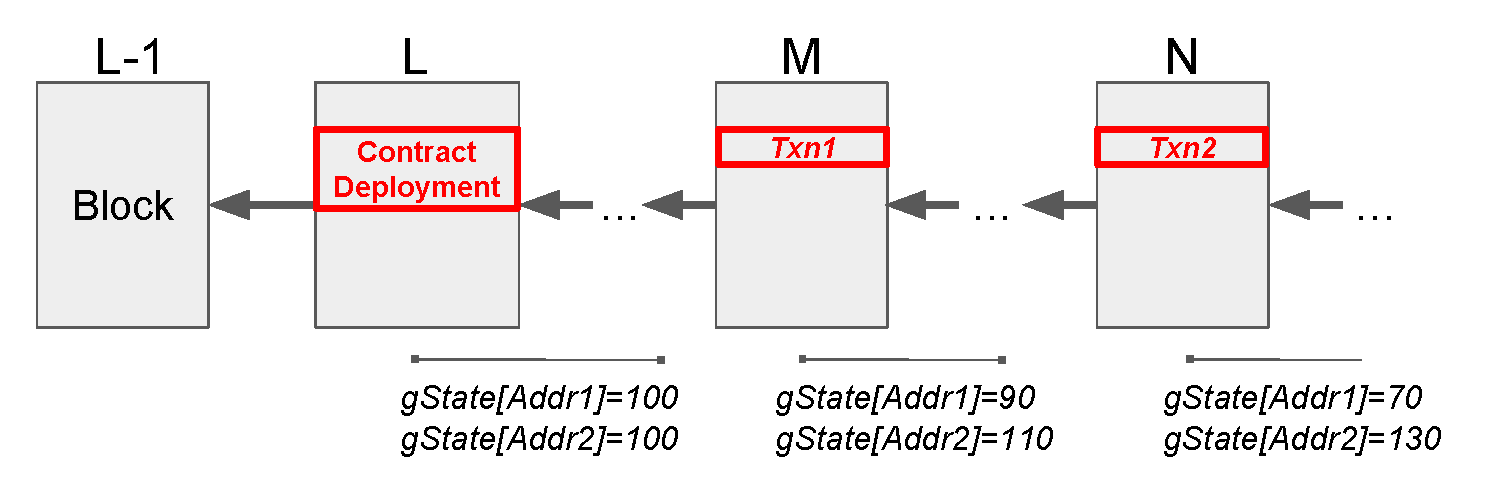
\includegraphics[width=0.9\textwidth]{diagram/provenance/contract.pdf}
  \caption{The example ledger with \textit{gState} between the block interval}
  \label{diagram:prov:ledger}
\end{figure}


\subsection{Capturing Provenance}
Blockchains support only a small set of data operators for general workloads, namely \textit{read} and \textit{write}. These operators are not provenance friendly, in the sense that they do not capture any data
association (input-output dependency). In contrast, relational databases or big data systems have many
provenance-friendly operators, such as \textit{map}, \textit{reduce} and \textit{join}, whose semantics meaningfully
capture the association. For instance, the output of \textit{join} is clearly derived from (or is dependent on)
the input data.  

\begin{figure}
    \footnotesize
    \centering
    \begin{verbatim}
    contract Token {
        method Transfer(...){...} // as above
        method prov_helper(name, reads, writes) {
          if name == "Transfer" {
            for (id,value) in writes {
                if (reads[id] < value) {
                    recipient = id;
                } else {sender = id; }
            }
            // dependency list with a 
            // single element. 
            dep = [sender];  
            return {recipient:dep};
          } 
          ...
        }
    }
    \end{verbatim}
    \caption{The provenance helper method for \textit{Token} contract}
    \subcaption*{It defines dependency between the
    sender identifier and recipient identifier. This method is invoke after every invocation of the Token
    contract.} 
    \label{code:prov:helper_contract}
\end{figure}


In {\fs}, every contract method can be made provenance-friendly via a {\em helper} method.  
More specifically, during transaction execution, {\fs} collects the identifiers and values of the
accessed states, i.e., ones used in \texttt{read} and \texttt{write} operations. The results are a read set \texttt{ 
reads} and write set \texttt{writes}. For {\em Txn1}, ${\texttt{reads}} = \{{\textit Addr1}: 100, {\textit Addr2}:
100\}$, and ${\texttt{writes}} = \{{\textit Addr1}: 90, {\textit Addr2}: 110\}$. After the execution finishes,
these sets are passed to a user-defined method \texttt{prov\_helper}, together with the name of the contract
method. \texttt{prov\_helper} has the following signature:
\begin{verbatim}
method prov_helper(name: string,
                   reads: map(string, byte[]), 
                   writes: map(string, byte[])) 
       returns map(string, string[]);
\end{verbatim}

It returns a set of dependencies based on the input read and write sets. Figure~\ref{code:prov:helper_contract}
shows implementation of the helper method for the Token contract. It first computes the identifier of the
sender and recipient from the read and write sets. Specifically, the identifier whose value in \texttt{writes} is lower than that
in \texttt{reads} is the sender, and the opposite is true for the recipient. It then returns a dependency set of
a single element: the recipient-sender dependency. In our example, for {\em Txn1}, this method returns
$\{{\textit Addr2}: [{\textit Addr1}]\}$ 

{\fs} ensures that \texttt{prov\_helper} is invoked immediately after every successfully contract execution.
If the method is left empty, {\fs} uses all identifiers in the read set as dependency of each identifier
in the write set. Interested readers may observe that the vanilla Fabric already computes for the read/write set
during the endorsement phase. 
Orthogonal to ours, they are internally used for the concurrency control to achieve one-copy serializability. 
Instead, we allow contract developers to capture for their application-level provenance. 


\subsection{Smart Contract APIs}
Current smart contracts can only safely access the {\em latest} blockchain state. In Hyperledger, for example, the \texttt{get(k)} operation returns the last value of $k$ that is written or being batched.  In Ethereum, on the other
hand, when a smart contract reads a value of $k$ at block $b$, the system considers the snapshot of states at
block $b-1$ as the latest states. Although there may exist a block $b' > b$ on a different branch, the
smart contract always treats what returned from the storage layer as the latest state.  

The main limitation of the current APIs is that the smart contract cannot tamper-evidently read previous values of a state.
Instead, the contract has to explicit track historical versions, for example by maintaining a list of versions
for every state. This approach is costly both in terms of storage and computation. {\fs} addresses this limitation with three additional smart contract APIs. 

\begin{itemize}
    \item \texttt{Hist(stateID, [blockNum])}: returns the tuple \texttt{(val, blkStart)} where \texttt{val}
    is the value of \texttt{stateID} at the snapshot of block \texttt{blockNum}. If \texttt{blockNum} is not specified, the latest block is used. \texttt{blkStart} is the index of the block that contains a transaction setting \texttt{stateID}. 

    \item \texttt{Backward(stateID, blkNum)}: returns a list of tuples \texttt{(depStateID, depBlkNum)} where \texttt{ depStateID} is the dependency state of \texttt{stateID} at block \texttt{blkNum}. \texttt{depBlkNum} is the block number at which the value of \texttt{depStateID} is set. It also returns \texttt{txID} which is the identifier of the transaction that sets \texttt{stateID}.
    In our example, \texttt{Backward(Addr2, N)} returns \texttt{(Addr1, M)} and \texttt{txID} is equal to \texttt{Txn2}. 

    \item \texttt{Forward(stateID, blkNum)}: similar to the \texttt{Backward} API, but returns the states of
    which \texttt{stateID} is a dependency and the corresponding transaction identifier. For example, \texttt{Forward(Addr1, L)} returns \texttt{(Addr2, M, Txn1)}.
\end{itemize}

\begin{figure}[t]
\footnotesize
\centering
\begin{verbatim}
contract Token {
  ...
  method Refund(addr) {
    blk := last block in the ledger
    first_blk := first block in this month
    sum = count = 0;
    while (first_blk < blk) {
      val, startBlk = Hist(addr, blk);
      blk = startBlk - 1; 
      sum += val;
      count += 1;
    }
    avg = sum / count;
    refund_amount := refund amount based on avg
    gState[addr] += refund_amount;
  }

  method Suspect(addr) {
    blk := last block in the ledger
    suspected = false;
    iterate 5 times {
      val, startBlk = Hist(addr, blk);
      for (depAddr, depBlk) 
            in (Backward(addr, startBlk) 
            or Forward(addr, startBlk)) {
        if depAddr in gState["suspect"] {
          gState["suspect"].append(addr);
          return;
        }
      }
      blk = startBlk - 1; 
    }
  }
}

\end{verbatim}
\caption{The modified \textit{Token} contract with provenance-dependent methods.}
\label{code:prov:enhanced_contract}
\end{figure}

% \subsection{Sample Usage}
Figure~\ref{code:prov:enhanced_contract} demonstrates how the above APIs are used to express smart contract logics
that are currently impossible in the secure manner.
We add two additional methods to the original contract, both of which use the new
APIs. The \textit{Refund} method examines an account's average balance in the recent month and makes the
refund accordingly. The \textit{Suspect} method marks an address as suspected if one of its last 5
transactions is with a suspected address. 



\section{Secure Provenance Storage} 
\label{sec:provenance:storage}
In this section, we discuss how {\fs} enhances existing blockchain storage layer to provide efficient
tracking and tamper evidence for the captured provenance. Our key insight is to reorganize the flat leaf
nodes in the original Merkle tree into a Merkle DAG. We first describe the Merkle DAG structure, then discuss
its properties. Finally, we explain how to exploit the blockchain execution model to support forward
provenance tracking. 

\subsection{Merkle DAG}

Let $k$ be the unique identifier of a blockchain state, whose evolution history is expected to be tracked. 
Let $v$ be the unique version number that identifies the state in its evolution history. 
When the state at version $v$ is updated, the new version $v'$ is strictly greater than $v$. 
In {\fs}, we directly use the block number as its version $v$. 
Let $s_{k,v}$ denote the value of the state with identifier
$k$ at version $v$. We drop the subscripts if the meaning of $k$ and $v$ are not important. For any $k \neq
k'$ and $v \neq v'$, $s_{k,v}$ and $s_{k',v'}$ represent the values of two different states at different versions.  
$s^b_k$ represents the state value with identifier $k$ at its latest version before block b. 
In our example, for $k=Addr1$ and $v=M$, $s_{k,v}=90$.

\begin{definition}
A transaction, identified by ${tid}$ which is strictly increasing, reads a set of input states $S^{i}_{tid}$ 
and updates a set of output states $S^{o}_{tid}$. 
A valid transaction satisfies the following properties: 
  \begin{equation}
    \label{eq:1} \forall s_{k_1,v_1}, s_{k_2,v_2} \in S^{o}_{tid}. \quad k_1 \ne k_2
    \land v_1 = v_2 
  \end{equation}
  \begin{equation}\label{eq:2}
    \forall s_{k_1,v_1} \in S^{i}_{tid}, s_{k_2,v_2} \in S^{o}_{tid}. \quad v_1 < v_2 
  \end{equation}
  \begin{equation}\label{eq:22}
    \forall s_{k,v} \in S^{i}_{tid},  s_{k,v'} \in S^{i}_{tid'}. \quad tid < tid' \Rightarrow v \le v'. 
  \end{equation}
  \begin{equation}\label{eq:3}
    tid \ne tid' \Rightarrow S^{o}_{tid} \cap S^{o}_{tid'} = \emptyset
  \end{equation}
\end{definition}

Property (\ref{eq:1}) means that the versions of all output states of a transaction are identical, 
because they are updated by the same transaction in the same block. 
Property (\ref{eq:2}) implies the version of any input state is strictly lower than
that of the output version. This makes sense because the blockchain establishes a total order over the
transactions, and because the input states can only be updated in previous transactions. 
Property (\ref{eq:22}) specifies that, for all the states with the same identifier, the input of later
transactions can never have an earlier version.  This ensures the input state of any transaction must be
up-to-date during execution time.  Finally, Property (\ref{eq:3}) means that every state update is  unique. 

\begin{definition}
The dependency of state $s$ is a subset of the input states of the transaction that outputs $s$. More
specifically: 
  \begin{displaymath}
    dep(s) \subset S^{i}_{tid} \ \text{where} \ s \in S^{o}_{tid}. 
  \end{displaymath}
\end{definition}
\noindent We note that $dep$, which is returned by \texttt{prov\_helper} method, is only a subset of the read
set.  

\begin{definition} \label{def:entry}
The entry $E_{s_{k,v}}$ of the state $s_{k,v}$ is a tuple containing the current version, the state value, and the
hashes of the entries of its dependent state. More specifically:
  \begin{displaymath}
    E_{s_{k,v}}= \langle v, s_{k,v}, \{hash(E_{s'})|s' \in dep(s_{k,v})\} \rangle
  \end{displaymath}
\end{definition}
\noindent An entry uniquely identifies a state. In {\fs}, we associate each entry with its corresponding
hash. 

\begin{definition}
The set of latest states at block $b$, denoted as $S_{latest,b}$ is defined as: 
  \begin{displaymath}
    S_{latest, b} = \bigcup\limits_{k}\{s^b_k\}
    % S_{latest, b} = \Union \{s^*_k\}
  \end{displaymath}
\end{definition}
\noindent Let $U_b$ be the updated states in block $b$. We can compute $S_{latest, b}$ by recursively
combining $U_b$ with $S_{latest, b-1} \setminus U_b$.  

\begin{definition}
$\chi_b$ is the root of a Merkle tree built on the map $S_b$ where 
  \begin{displaymath}
  S_b = \{k:hash(E_{s^b_{k}}) | \forall s^b_{k} \in S_{latest, b}\}. 
  \end{displaymath}
\end{definition}

{\fs} stores $\chi_b$ as the state digest in the block header. Figure~\ref{diagram:prov:dag} illustrates how state DAG evolves with the blockchain.

\begin{figure}
  \centering
  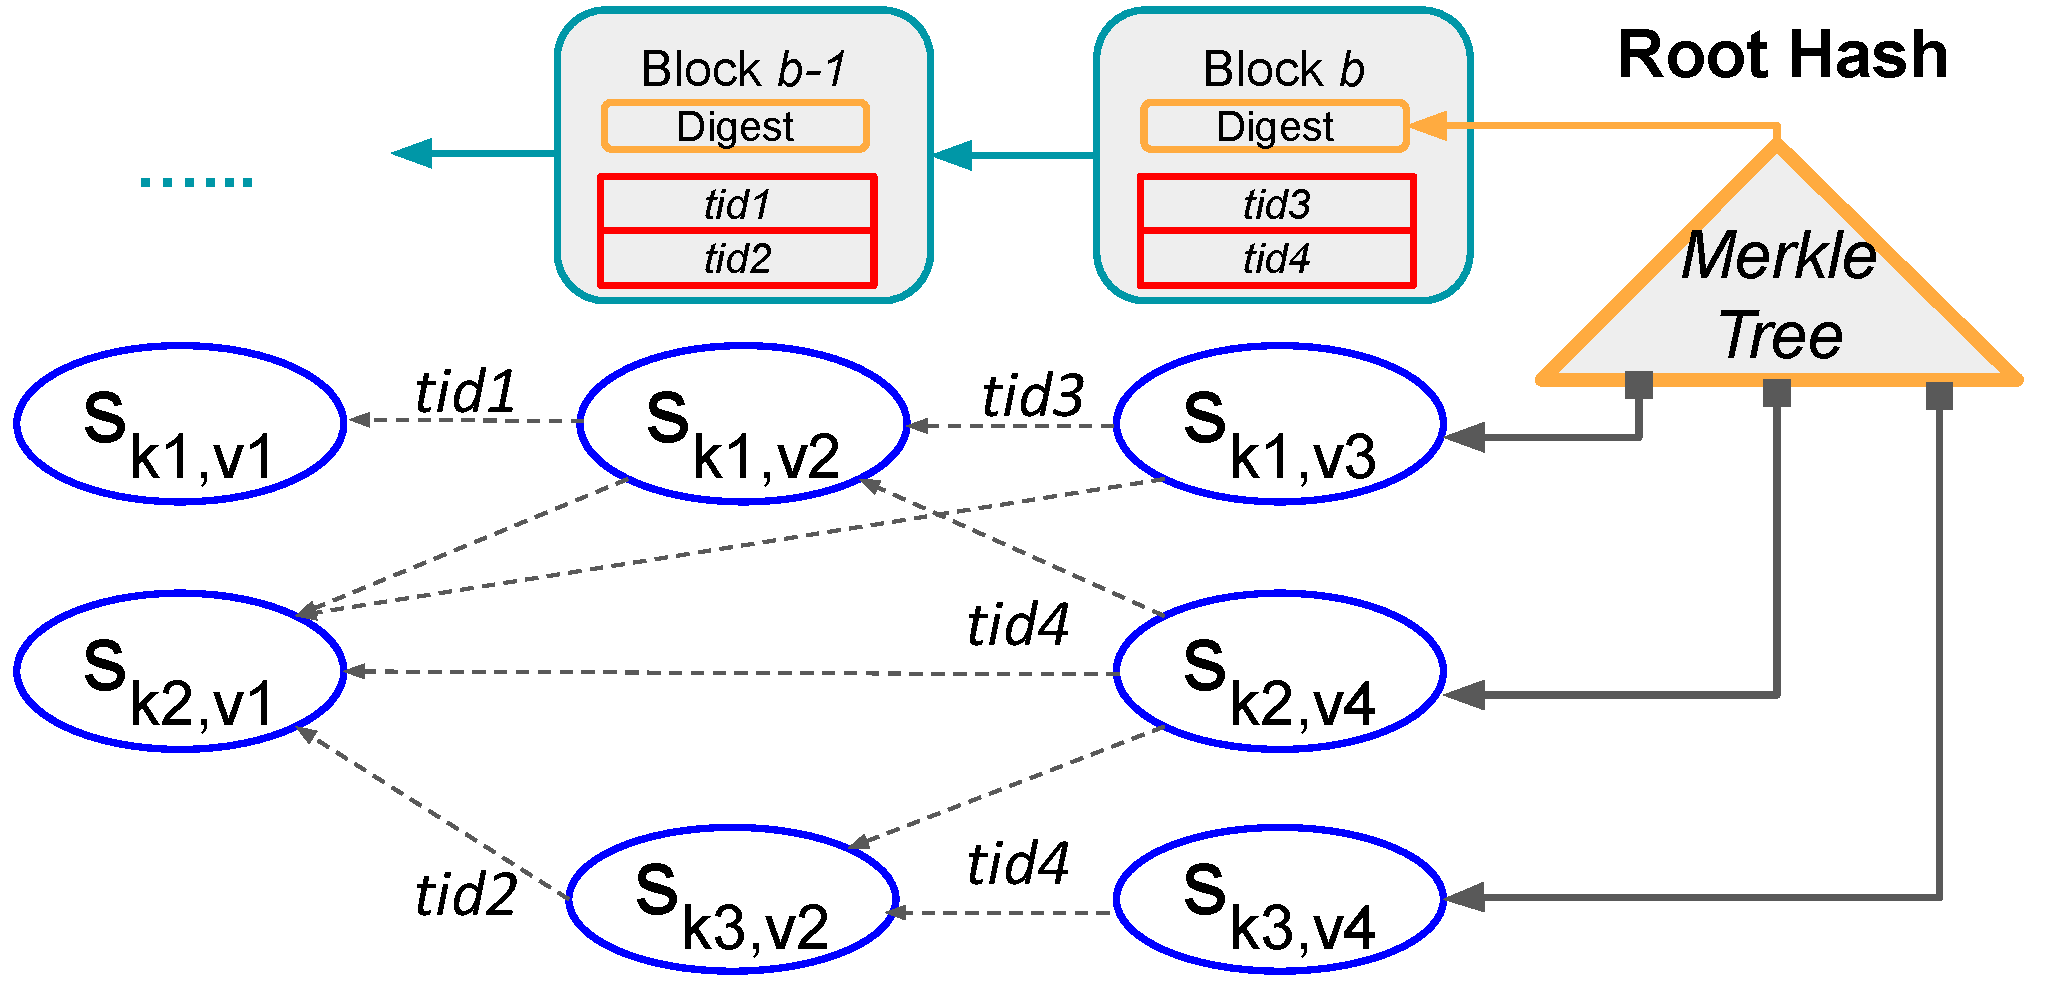
\includegraphics[width=0.9\textwidth]{diagram/provenance/DAG.pdf}
\caption{A Merkle DAG for storing provenance. }
\subcaption*{$s_{k_2,v_4}$ and $s_{k_3,v_4}$ updated by the same transaction ($tid_4$), but their dependencies are
different. $b$ contains two transactions, $tid_3$ and $tid_4$. Its latest states include $s_{k_1,
v_3}$, $s_{k_2,v_4}$, $s_{k_3,v_4}$, from which a Merkle tree is built.} 
\label{diagram:prov:dag} 
\end{figure}

\subsection{Discussion}
Our new Merkle DAG can be easily integrated to existing blockchain index structures. In particular, existing
Merkle index such as MPT stores state values directly at the leaves, whereas the Merkle DAG in {\fs} stores
the entry hashes of the latest state versions at the leaves. By adding one more level of indirection, we
maintain the three properties of the index (tamper evidence, incremental update and snapshot), while enhancing
it with the ability to traverse the DAG to extract fine-grained provenance information. 

Recall that the state entry hash captures the entire evolution history of the state. Since this hash is
protected by the Merkle index for tamper evidence, so is the state history.  In other words, we add integrity
protection for provenance without any extra cost to the index structure.  For example, suppose a
client wants to read a specific version of a state, it first reads the state entry hash at the latest block.
This read operation can be verified against tampering, as in existing blockchains. Next, the client traverses
the DAG from this hash to read the required version. Because the DAG is tamper evident, the integrity of the
read version is guaranteed.

\subsection{Support for Forward Tracking}
\label{sec:provenance:storage:forward}
One problem of the above DAG model is that it does not support forward tracking, because the hash pointers
only reference {\em backward} dependencies. When a state is updated, these backward
dependencies are permanently established, so that they belong to the immutable derivation history of the
state. However, the state can be read by future transaction, therefore its forward dependencies cannot be
determined at the time of update. 

\begin{figure}
  \centering
  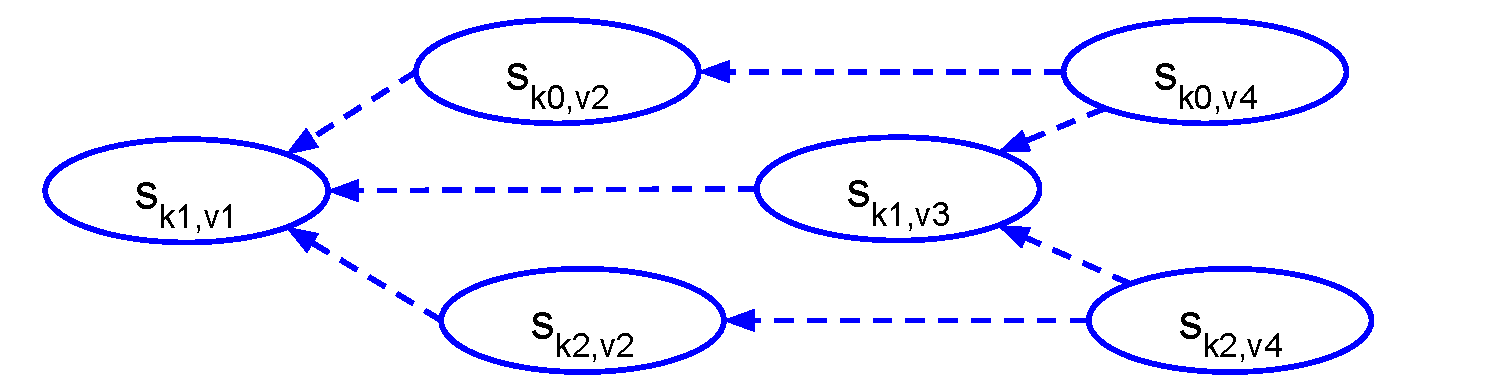
\includegraphics[width=0.9\textwidth]{diagram/provenance/forward.pdf}
  \caption{Forward tracking support for data provenance}
  \label{diagram:prov:forward}
  \subcaption*{After $s_{k_1,v_1}$ is updated, there can only be $s_{k_0,v_2}$ and
  $s_{k_2,v_2}$ that are dependent on $s_{k_1,v_1}$. Future states can only depend on $s_{k_1,v3}$. Forward
  pointers of $s_{k_1,v_1}$ are stored in the entry of $s_{k_1,v_3}$. } 
\end{figure}

Our key insight here is that only forward dependencies of the {\em latest state} are mutable. Once the state
is updated, due to the execution model of blockchain smart contract, in which the latest state is always read,
forward dependencies of the previous state version becomes permanent. As a result, they can be included into
the derivation history. Figure~\ref{diagram:prov:forward} illustrates an example, in which forward dependencies of
$s_{k_1, v_1}$ becomes fixed when the state is updated to $s_{k_1, v_3}$. This is because when the transaction
that
outputs $s_{k_0, v_4}$ is executed, it reads $s_{k_1, v_3}$ instead of $s_{k_1, v_1}$. 

In {\fs}, for each state $s_{k,v}$ at its latest version, we buffer a list of forward pointers to the
entries whose dependencies include $s_{k,v}$.  We refer to this list as $F_{s_{k,v}}$, which is defined more precisely as
follows: 
\begin{displaymath}
F_{s_{k,v}} = \{hash (E_{s'}) | s_{k,v} \in dep(s')\}
\end{displaymath}
\noindent When the state is updated to $s_{k,v'}$ for $v' > v$, we store $F_{s_{k,v}}$ at the entry of
$s_{k,v'}$.  

\section{Efficient Provenance Queries}
\label{sec:provenance:index}
The Merkle DAG structure supports efficient access to the latest state version, since the state index at block
$b$ contains pointers to all the latest versions at this block. To read the latest version of $s$, one simply
reads $\chi_b$, follows the index to the entry for $s$, and then reads the state value from the entry.
However, querying an arbitrary version in the DAG is inefficient, because one has to start at the DAG head
and traverse along the edges towards the requested version.  Supporting fast version queries is important
when the user wants to examine the state history only from a specific version (for auditing purposes, for
example).  It is also important for provenance-dependent smart contracts because such queries directly affect
contract execution time. 

In this section, we describe a novel index that facilitates fast version queries. The index is designed for
permissioned blockchains. We discuss its efficiency and how to extend it to permissionless blockchains. 

\subsection{Deterministic Append-Only Skip List} 
We propose to build an index on top of a state DAG to enable fast version queries. The index has a skip list
structure, which we call Deterministic Append-only Skip List (or DASL). It is designed for blockchains,
exploiting the fact that the blockchain is append-only, and randomness is not well
supported~\cite{cachin2016non}. More specifically, a DASL has two distinct properties compared to a normal skip
list. First, it is append-only. The index keys of the appended items, which are versions in our case, are
strictly increasing. Second, it is deterministic, that is,
the index structure is uniquely determined by the values of the appended items, unlike a stochastic skip list.
For ease of explanation, we assume that version numbers are positive integers.

\begin{definition}\label{def:1}
  Let $V_k = \langle v_0, v_1, ...\rangle$ be the sequence of version numbers of states with identifier $k$, in which $v_i <
  v_j$ for all $i<j$. A DASL index for $k$ consists of $N$ linked lists $L_0, L_1,.., L_{N-1}$. Let $v^{i}_{j-1}$ and $v^i_j$ be
  the versions in the $(j-1)^{\textit{th}}$ and $j^{\textit{th}}$ node of list $L_i$. Let $b$ be the base number, a system-wide parameter. The content
  of $L_i$ is constructed as follows:
 
  1) $v_0 \in L_i$

  2) Given $v^i_{j-1}$, $v^i_j$ is the smallest version in $V_k$ such that: 
  \begin{equation}\label{eq:4}
    \floor*{\frac{v^i_{j-1}}{b^i}} < \floor*{\frac{v^i_j}{b^i}}
  \end{equation}
\end{definition}

\begin{figure}
  \centering
  \footnotesize
  \begin{verbatim}
  struct Node {
    Version v;
    Value val;
    List<Version> pre_versions;
    List<Node*> pre_nodes;
  }
  \end{verbatim}
  \caption{Node structure that captures a state $s_{k,v}$ with value $val$}
  \label{code:prov:node}
\end{figure} 

\begin{figure}
  \centering
  \begin{subfigure}{0.32\textwidth}
    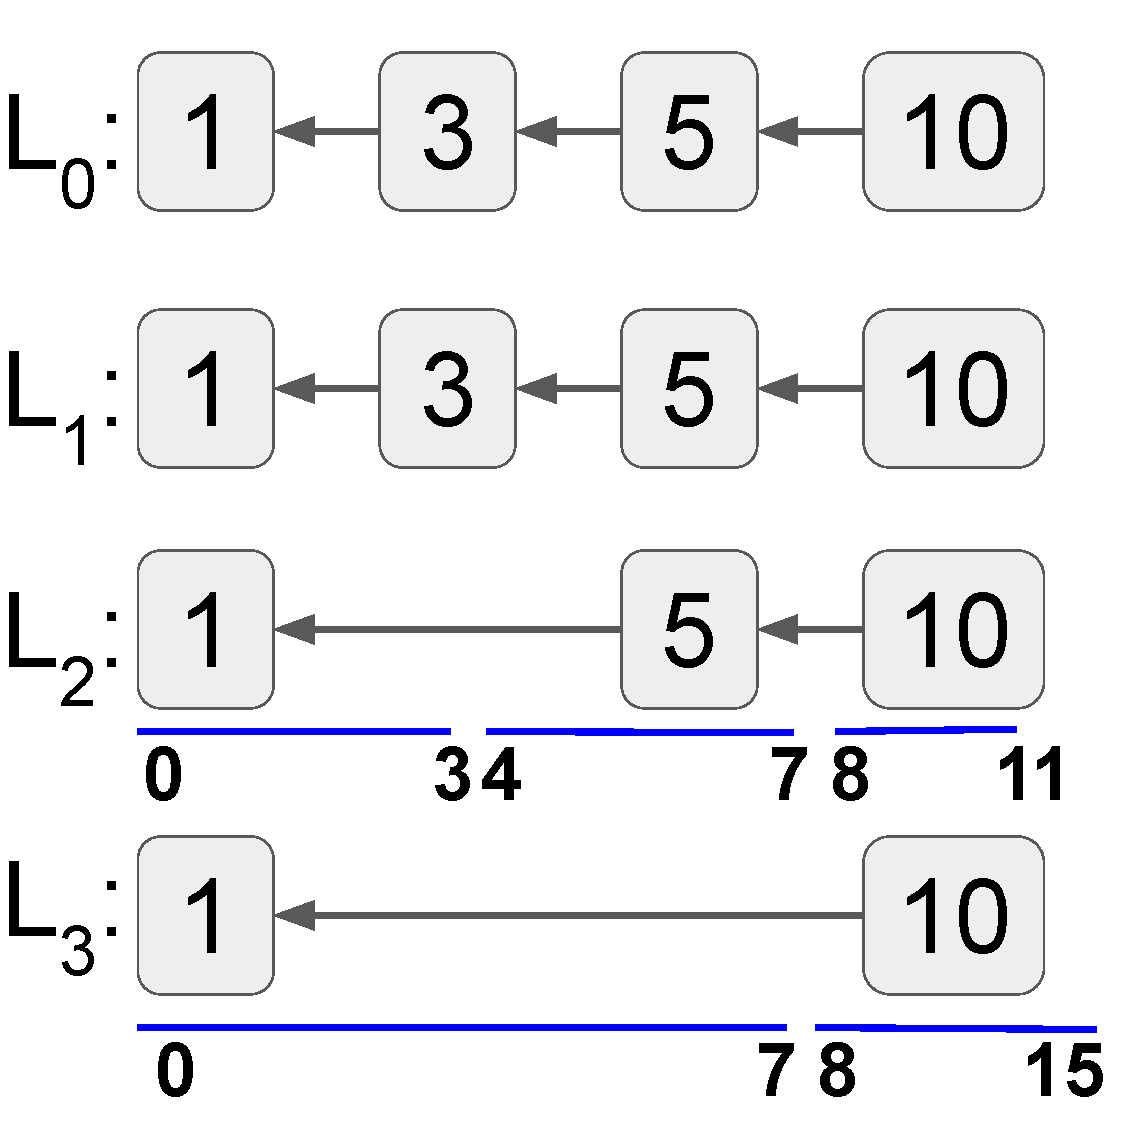
\includegraphics[width=0.99\textwidth]{diagram/provenance/dasl_original.pdf}
    \caption{}
    \label{diagram:prov:dasl_original}
  \end{subfigure}
  \begin{subfigure}{0.54\textwidth}
    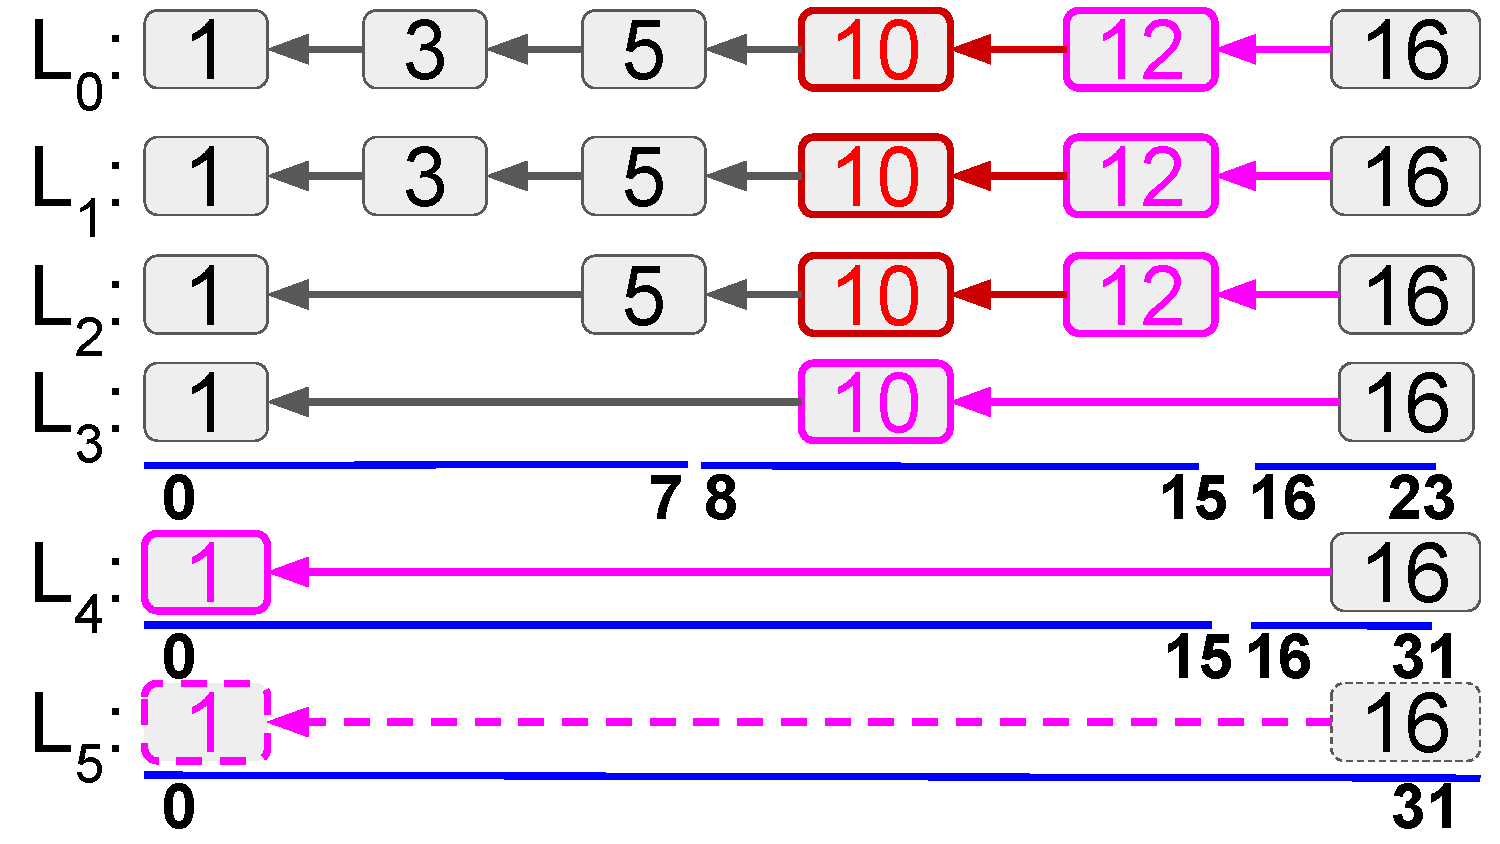
\includegraphics[width=0.99\textwidth]{diagram/provenance/dasl_appended.pdf}
    \caption{}
    \label{diagram:prov:dasl_appended}
  \end{subfigure}
  \caption{An example of the append procedure in Deterministic Append-only Skip List (DASL)}
  \subcaption*{(a) A DASL containing versions 1, 3, 5 and 10. The base $b$ is 2. The intervals for $L_2$ and
  $L_3$ are shown in blue lines. (b) The new DASL after appending version 12 and 16. $L_4$ is created when appending version $16$. $L_5$ is created, then discarded.} 
\end{figure}

Figure~\ref{code:prov:node} shows how DASL is stored with the state in a data structure called Node.  This structure
(also referred to as node) consists of the state version and value. A node belongs to multiple lists (or
levels), hence it maintains  a list of pointers to some version numbers, and another list of pointers to other
nodes.  Both lists are of size $N$, and the $i^{\textit th}$ entry of a list points to the previous version
(or the previous node) of this node in level $L_i$.  For the same key, the version number uniquely identifies
the node, hence we use version numbers to refer to the corresponding nodes.

We can view a list as consisting of continuous, non-overlapping intervals of certain sizes. In particular, the
$j^{\textit{th}}$ interval of $L_i$ represents the range $R^i_j = [jb^i, (j+1)b^i)$. Only the smallest version in $V_k$ that
falls in this range is included in the list. Figure~\ref{diagram:prov:dasl_original} gives an example of a DASL
structure with $b=2$. It can be seen that when the version numbers are sparsely distributed, the lists at lower levels are
identical. In this case, $b$ can be increased to create larger intervals which can reduce the overlapping among
lower-level lists.   

A DASL and a skip list share two properties. First, if a version number appears in $L_i$, it also appears in
$L_j$ where $j<i$.  Second, with $b=2$, suppose the last level that a version appears in is $i$, then this
version's preceding neighbour in $L_i$ appears in $L_j$ where $j>i$. 
Given these properties,
a query for a version in the DASL is executed in the same way as in the skip list.
More specifically, the query traverses a high-level list as much as possible, starting from
the last version in the last list. It moves to a lower level only if the preceding version in the current list
is strictly smaller than the requested version. In DASL, the query for version $v_q$ returns the largest
version $v \in V_k$ such that $v \leq v_q$ (the inequality occurs when $v_q$ does not exist). This result
represents the value of the state which is visible at time of $v_q$. 

\begin{algorithm}[t]
  \caption{DASL Append}
  \label{alg:prov:append}
  %uint b \tcp{base}
  \KwIn{version $v$ and last node $last$}
  \KwOut{previous versions and nodes}
  $\textit{level}$=0;\   \tcp{list level} 
  $\textit{pre\_versions}$ = []\;
  $\textit{pre\_nodes}$ = []\;
  $\textit{finish}$ = false \;
  $\textit{cur} = \textit{last}$ \;
  \While{not finish} {
    $l$ = $\textit{cur}$->$\textit{pre\_versions.size()}$ \;
    \If {l > 0} {
      \For {j=level; j<l; ++j} { \label{alg:prov:append:iterate_begin}
        \If {$\textit{cur}$->$\textit{version}$ / $b^j$ < $v$ / $b^j$} {
          $\textit{pre\_versions}$.append($\textit{cur}$->$\textit{version}$)\;
          $\textit{pre\_nodes}$.append($\textit{cur}$)\;
        } \Else {
          $\textit{finish}$ = true\;
          break\;
        }
      }
      \If {not finish} {
        $\textit{cur}$ = $\textit{cur}$->\textit{pre\_versions[l-1]}\;
        $\textit{level}=l$
      } \label{alg:prov:append:iterate_end}
    } \Else {
      \tcc {We have reached the last level}
      $\textit{finish}$ = true\;
      \While {$\textit{cur}$->$\textit{version}$ / $b^{\textit{level}}$ < $v$ / $b^{\textit{level}}$} { \label{alg:prov:append:head_begin}
        ++$\textit{level}$\;
        $\textit{pre\_versions}$.append($\textit{cur}$->$\textit{version}$)\;
        $\textit{pre\_nodes}$.append($\textit{cur}$)\;
      }\label{alg:prov:append:head_end}
    }
  }

  \Return{$pre\_version$, $pre\_nodes$;}
\end{algorithm}

We now describe how a new node is appended to DASL. The challenge is to determine the lists that should include the
new node. Algorithm \ref{alg:prov:append} details the steps that find the lists, and subsequently the previous
versions, of the new node. The key idea is to start from the last node in $L_0$, then keep increasing the list
level until the current node and the new node belong to the same interval (line
\ref{alg:prov:append:iterate_begin} - \ref{alg:prov:append:iterate_end}). Figure~\ref{diagram:prov:dasl_appended} shows the result of appending a node with version $12$ to the original DASL. The algorithm starts at node $10$ and moves up to list $L_1$ and $L_2$. It stops at $L_3$ because in this level node $10$ and $12$ belong to the same
interval, i.e., $[8,16)$. Thus, the new node is appended to list $L_0$ to $L_2$. When the algorithm reaches
the last level and is still able to append, it creates a new level where node $0$ is the first entry and
repeats the process (line \ref{alg:prov:append:head_begin} -
\ref{alg:prov:append:head_end}). In Figure~\ref{diagram:prov:dasl_appended}, when appending version $16$, all existing lists can be used. The algorithm then creates $L_4$ with node $1$ and appends the node $16$ to it. It also creates
level $L_5$, but then discards it because node $16$ will not be appended since it belongs to same
interval of $[0,32)$ with node $1$. 

\subsection{Discussion} \label{sec:provenance:model_discuss}
\textbf{Integrating to Merkle DAG. } 
The DASL is integrated to the Merkle DAG as follows. The node structure (Figure \ref{code:prov:node}) is stored in
the state entry (Definition~\ref{def:entry}).  The node pointers are implemented entry hashes. The Merkle tree
structure remains unchanged.  

\textbf{Speed-storage tradeoff. } 
As a skip list variant, DASL shares the same lineage space complexity and 
logarithmic query time complexity. 
Suppose there are $v^*$ number of versions and the base of DASL is $b$. 
The maximum number of required pointers is $\frac{bv^*-1}{b-1}$. 
(There are at most $\ceil{\log_b v^*}$ levels and the $i$-th level takes at most $\ceil{\frac{v^*}{b^i}}-1$ pointers.)
Suppose the queried version is $v^q$ and the query distance $d=v^*-v^q$, the maximum number of hops in such query is capped at $2b\ceil{\log_b d}$. (A query traversal from the end will undergo two stages, one stage towards lower levels  and the other stage back towards upper levels. In each stage, 
the traversal will take at most $b$ hops on the same list before moving to the next level.
And there are at most $\ceil{\log_b d}$ levels to traverse.)
Hence, $b$ controls the tradeoff between the space overhead and query delay. 
One benefit of this property is that DASL queries favor more recent
versions, i.e. $d$ are small.
It is useful for smart contracts that work on recent rather than old versions.  
Another benefit is that the performance of such recent-version queries does not change as the state history grows.  

\textbf{Extending to permissionless blockchains. } 
We note that DASL incurs storage overhead. The version query also incurs some computation cost, even though it
is more efficient with DASL than without it. These costs may be small enough such that they do not
affect the performance of a permissioned blockchain, as we demonstrate in \Cref{sec:provenance:exp}.  However,
they need to be carefully managed in a permissionless blockchain where any overhead directly translates to
monetary cost to the miners. In particular, any additional cost to the miner triggers the Verifier
Dilemma~\cite{luu2015demystifying} and compromises the incentive mechanism of the blockchain.  

A malicious user could issue a transaction that references a very old version. Reading earlier versions is more
expensive, because there are more hops involved. This overhead is born by all nodes in the network,
since every node in the network has to execute the same transaction. Current public blockchains prevent such
denial-of-service attack by explicitly charging a fee for each operation in the transaction. In Ethereum, the
transaction owner pays for the resource consumption in {\em gas}. A transaction that writes more data or
consumes more CPUs has to pay more {\em gas}. Thus, rational users are deterred from running too complex
transactions on the blockchain. 

As DASL consumes resources, its costs must be explicitly accounted for in permissionless blockchains.
More specifically, during deployment, the contract owner specifies which states require DASL support.
Alternatively, DASL support can be automatically inferred from the contract's source code. The deployment fee
should reflect this extra storage cost for DASL. If the fee is too high, the owner can lower it by increasing
b. During contract execution, the execution engine must charge the cost of DASL queries to the transaction
fee. In particular, a query that requires more hops to find the requested version incurs a higher transaction
fee. Users may empirically estimate the hops (as well as the cost) based on the above-derived theoretical upper bound. 

\section{Implementation}
\label{sec:provenance:implementation}
\begin{figure}
  \centering
  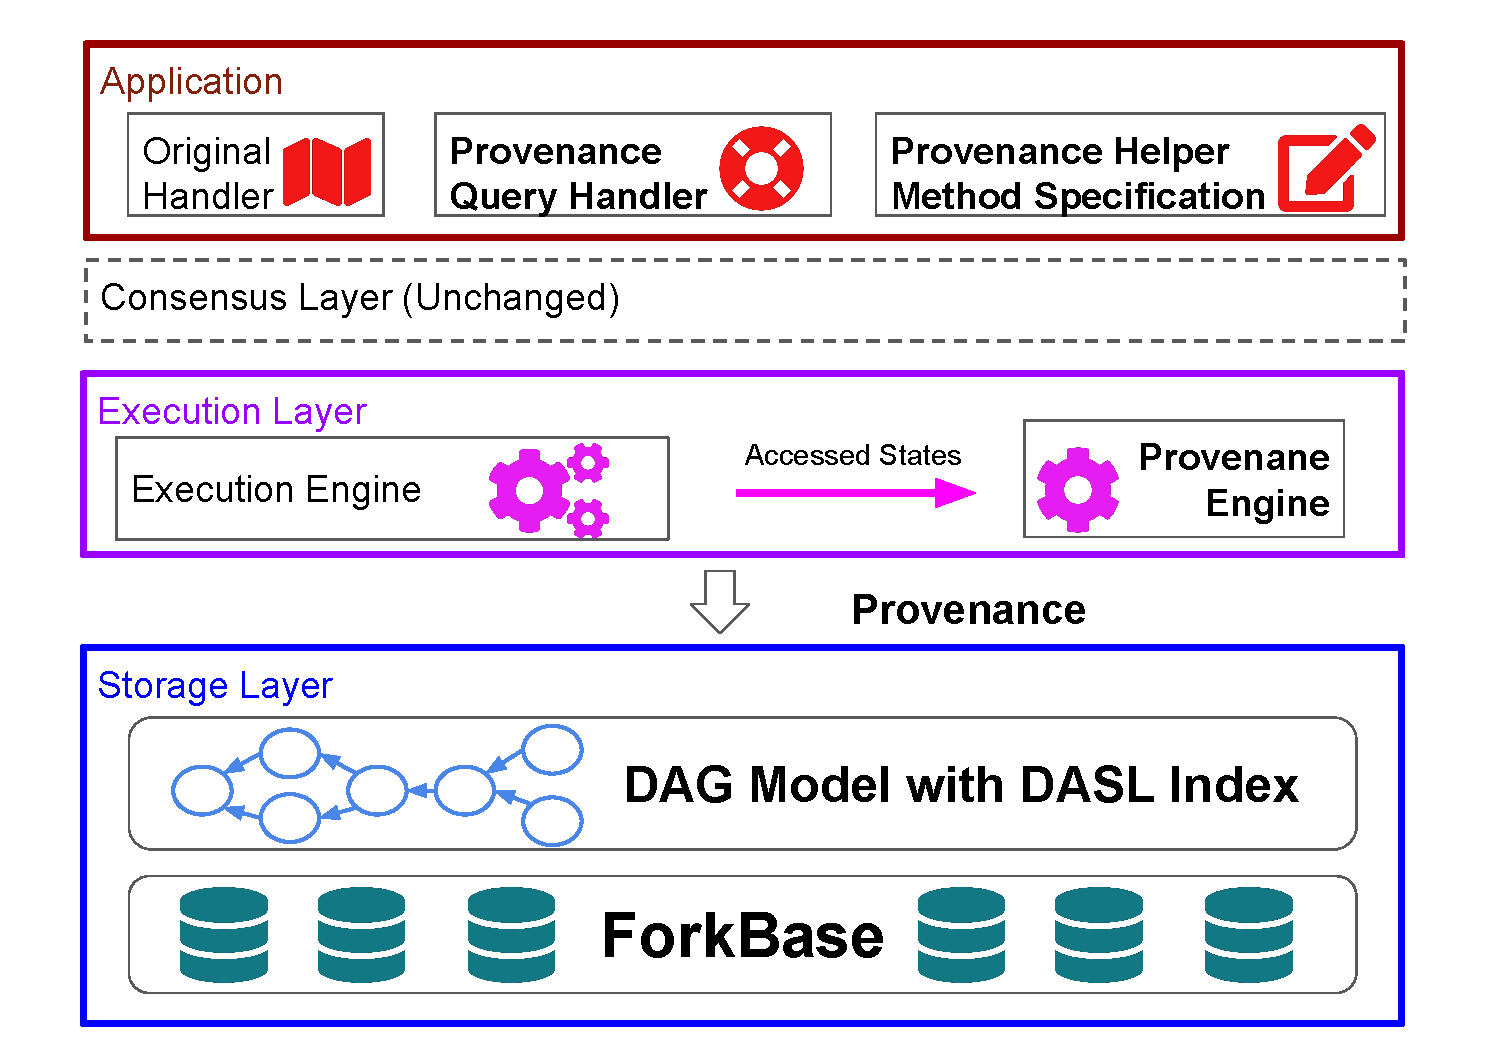
\includegraphics[width=0.8\textwidth]{diagram/provenance/lineagechain.pdf}
  \caption{The {\fs}'s instrumentation on Fabric to support data provenance }
  \subcaption*{The original storage layer is replaced with the implementation that
  supports fine-grained provenance. The original execution layer is instrumented with a provenance capture
  engine. The application layer contains the new helper method and provenance query APIs. The consensus layer is unchanged. } 
  \label{diagram:prov:arch} 
\end{figure}

\begin{algorithm}
  \caption{Provenance update and digest Computation} \label{prov:fabric_change} 
  \tcc{fb is the shorthand for ForkBase. fb.Map is the built-in map data type in Forkbase.}     
  fb.Map<id,vid> $\textit{latest}$\;
    String $\textit{branch}$ = "default"\;
    \tcp{Buffered forward pointers}
    Map<id, List<vid>> $\textit{forward}$\;  
  
    \KwIn{$\textit{id}$, $\textit{version}$, $\textit{value}$ of the updated state}
    \KwIn{ids of the dependent states, $\textit{dep\_ids}$}
    \SetKwFunction{FUpdate}{Update}
    \SetKwProg{Fn}{Function}{:}{}
    \Fn{\FUpdate{id, version, value, dep\_ids}}{
     \tcc {Backward pointers}
      List<vid> $\textit{back\_vids}$\; \label{lst:line:back_begin}
      \For {$\textit{dep\_id}$ in $\textit{dep\_ids}$} {
        $\textit{back\_vid}$ = $latest$[$\textit{dep\_id}$]\;
        $\textit{back\_vids}$.push\_back($\textit{back\_vid}$)\;
      } \label{lst:line:back_end}
      \tcc{Forward pointers}
      $\textit{forward\_vids}$ = $\textit{forward[id]}$\; \label{lst:line:forward}
      \texttt{\\}
   
      \tcc{Retrieve pointer to last DASL node}
      $\textit{last\_vid}$ = $latest$[$\textit{id}$]\;  \label{lst:line:dasl_begin}
      \tcc{Refer DASL Append in Algorithm \ref{alg:prov:append}}
      $\textit{pre\_versions}$, $\textit{pre\_vids}$ = DaslAppend($\textit{version}$, $\textit{last\_vid}$)\; 
      $\textit{node}$ = new DaslNode\{$version$, $pre\_versions$, $pre\_vids$\} \;\label{lst:line:dasl_end}
      $\textit{meta}$ = Serialize($\textit{back\_vids}$, $\textit{forward\_vids}$, $node$) \;  \label{lst:line:dump_begin}
  
      \texttt{\\}
      \tcc{Store the updated value}
      $\textit{new\_vid}$ = fb.Put($\textit{id}$, $\textit{branch}$, $\textit{value}$, $\textit{meta}$)\;  \label{lst:line:dump_end}
  
      \texttt{\\}
      \tcc{Update forward pointers}
      \For {$\textit{dep\_id}$ in $\textit{dep\_ids}$} {  \label{lst:line:forward_begin}
        $\textit{forward[dep\_id]}$.push\_back($\textit{new\_vid}$);
      }
  
      $\textit{forward[id]}$.Clear()\;  \label{lst:line:forward_end}
      $\textit{latest[id]}$ = $\textit{new\_vid}$\;  \label{lst:line:latest}
    }
    \texttt{\\}
    \KwOut{The state digest for the committed block}
    \SetKwFunction{FCommit}{ComputeDigest}
    \Fn{\FCommit{}}{
      $\textit{latest\_vid}$ = fb.Put("state", $\textit{branch}$, $\textit{latest}$, nil)\;
      \Return{$\textit{latest\_vid}$}\;
    }
\end{algorithm}
In this section, we present our implementation of {\fs} based on Hyperledger Fabric v2.2. 
Figure~\ref{diagram:prov:arch} highlights our changes in a layer-wise fashion. 
In particular, we completely
replace the storage layer with our implementation of the Merkle DAG and DASL index. This new storage
is built on top of ForkBase~\cite{wang2018forkbase}, a state-of-the-art blockchain storage system
with support for version tracking.  We instrument the original execution engine to record read and write sets
during contract execution. At the application layer we add a new helper method and three provenance APIs. The
execution engine is modified to invoke the helper method after every successful contract execution.  


\subsection{Storage Layer}
Instead of implementing the storage layer from scratch, we leverage ForkBase for its support of version
tracking.  We exploit three properties of ForkBase in {\fs}. The first is the fork semantics, with which
the application can specify a \textit{branch} for the update. Given
a branch, ForkBase provides access to the latest value.  The second property is tamper evidence, in which
every update returns a tamper-evident identifier {\em vid} which captures the entire evolution history of the
updated value. A data object in ForkBase is uniquely identified by the key and {\em vid}. In {\fs}, {\em
vid} is used as the entry hash in the DAG, and as the pointer in DASL. The third property is the rich set of
built-in data types including map, list and set. 
Figure~\ref{code:prov:api} lists our utilized ForkBase APIs with their explanations. 

\begin{figure}
\centering
\footnotesize
\begin{verbatim}
// Update the value for key in a branch with the metadata 
//   and return a tamper-evident vid. 
// Value can be a primitive like a string, or more complex types like map, list, etc. 
vid <- Put(key, branch, value, metadata);
// Retrieve the latest value for a key on a branch
value <- GetLastValue(key, branch);
// Retrieve the value or the metadata for a key based on vid. 
value <- GetValue(key, vid);
meta <- GetMetadata(key, vid);
\end{verbatim}
\caption{ForkBase APIs to implement the {\fs}'s storage}
\subcaption{\textit{metadata} is a user provided string that describes the updated value. And \textit{vid} is uniquely determined by the updated value, key, branch and the metedata. }
\label{code:prov:api}
\end{figure}

Algorithm~\ref{prov:fabric_change} details our implementation for updating states
and computing the global state digest when a block is being
committed. The update function is invoked with a new state
and a list of dependencies. We first prepare the list of backward pointers by retrieving the latest {\em vids} of the dependent
states (line~\ref{lst:line:back_begin}-\ref{lst:line:back_end}). Next, we build the pointers for the DASL
index, then retrieve the forward pointers
of the previous state (line~\ref{lst:line:forward}). The metadata from these steps are serialized and stored together with the updated
value in ForkBase (line~\ref{lst:line:dump_begin}-\ref{lst:line:dump_end}). The result is a new {\em vid} for
the update, which is appended to the list of forward pointers of every dependent state
(line~\ref{lst:line:forward_begin}-\ref{lst:line:forward_end}). {\em vid} is now 
the latest version (line \ref{lst:line:latest}). 

The global states are stored in a map object in ForkBase. To compute the global state digest, we simply update
the map object with the new {\em vids} computed for this block. The update operation of the map object, which
is built as a Merkle tree in ForkBase, returns a digest {\em latest\_vid} which is then included
to the block header.  This digest provides tamper evidence for the evolution histories of all the states up to
the current block.
Given a {\em key}, the query on its latest value can be directly answered by \textit{fb.GetLastValue(key, branch="default")}. For the historical value and dependency, one must locate the corresponding {\em vid} for that entry. 
DASL facilitates this query process. 
Then one shall use {\em vid} to fetch for the value and metadata with the corresponding ForkBase APIs. 

\subsection{Application and Execution Layer}
In {\fs}, users write their smart contracts by implementing the \texttt{Chaincode} interface. Given any  \texttt{Chaincode} implementations, the execution engine triggers the \texttt{Init} and \texttt{Invoke} method during deployment and
invocation respectively. Both methods take as input an instance of \texttt{ChaincodeStubInterface} which
supplies relevant context, such as access to the ledger states, to the smart contract. 

We add the helper method, called \texttt{ProvHelper}, to the \texttt{Chaincode} interface. This method's signature,
and how to write user-defined provenance rules with it, are explained in \Cref{sec:provenance:capture}. The
execution engine intercepts \texttt{PutState} and \texttt{GetStates} during execution to record the read set and the
write set. It invokes \texttt{ProvHelper} when the execution finishes. Then it piggybacks the computed dependency along with the transaction, later to be stored securely when the transaction commits. Fig
The three new provenance APIs, namely \texttt{Hist}, \texttt{Backward} and \texttt{Forward}, are added to \texttt{ChaincodeStubInterface}
and therefore previously-stored provenance is accessible to all contract methods. 


\section{Performance Evaluation}
\label{sec:provenance:exp}
\subsection{Baselines and Experimental Setup}
\label{sec:provenance:exp:setup}

We evaluate {\fs} against two baselines. 
The first baseline is the original Fabric, without any provenance support.
The second one, which we refer as {\fsPr}, directly enhances the original storage engine LevelDB for the provenance. 
To be specific, previously Fabric associates the state IDs only with their latest values in LevelDB. 
With our modification, historical values and dependencies are now associated with the concatenations of their IDs and versions. 
For example, with respect to the example in Figure~\ref{diagram:prov:dag}, the storage entries (in the format of \textit{key:value}) for state ID $k_1$ are organized as follows: 
\begin{equation*}
  \begin{aligned}
    Hist\_k1\_v1: S_{k1\_v1} \\
    Hist\_k1\_v2: S_{k1\_v2} \\
    Hist\_k1\_v3: S_{k1\_v3} \\
    Backward\_k1\_v1: \{\} \\
    Backward\_k1\_v2: \{k1\_v1,k2\_v1\} \\
    Backward\_k1\_v3: \{k1\_v2,k2\_v1\} \\
    Forward\_k1\_v1: \{k1\_v2\} \\
    Forward\_k1\_v2: \{k1\_v3, k2\_v4\} \\
    Backward\_k1\_v3: \{\} \\
  \end{aligned}
\end{equation*}
With the help of built-in LevelDB iterator, such flat organization facilitates the provenance retrieval for states at a specific version. 
However, compared with our ForkBase in {\fs}, it does not protect the provenance integrity, nor does it support the discriminated version retrieval as our DASL. 
Despite the storage differences, {\fsPr} is similar with {\fs}, i.e., both share the exact provenance capturer and query handlers. 

We perform three sets of experiments. First, we repeat the YCSB and Smallbank experiments to evaluate the performance implication with the provenance support. 
Secondly, we demonstrate the provenance-provided utility with the Smallbank workload. In the meantime, we dissect the Fabric bottleneck (the validation phase as identified in Chapter~\ref{sec:twin:exp:replication:model}) to understand the exact overhead. 
In the remaining experiments, we place a specific analysis on the provenance query and space consumption of the storage engine. 
Note that in the following paragraphs and charts throughout this chapter, we refer {\fsPr} as {\fsPrO} and {\fs} as {\fsO}. The additional suffix \textit{O} denote that both Fabric variants use the original transaction scheduler. 
We vary the transaction scheduler in the next chapter. 

\subsection{Peak Performance}
\label{sec:provenance:exp:peak}

Figure~\ref{chart:provenance:basic} presents the effective throughput for YCSB and Smallbank at their respective optimal setup, as previous identified in Chapter~\ref{sec:intro:basis}. 
In the YCSB experiment, {\fsPrO} and {\fsO} track each value of for all historical versions of records, while the original Fabric only maintains the latest state. 
For Smallbank, we implement the provenance helper method (which is detailed in Chapter~\ref{sec:provenance:capture}) to capture the monetary flow. 
So besides the historical versions, {\fsPrO} and {\fsO} also preserve the dependency information. 
Despite all these provenance features, we observe from Figure~\ref{chart:provenance:basic} that the performance overhead is negligible. 
To be specific, under 1000 transactions per block with the YCSB workload, Fabric, {\fsPrO} and {\fsO} respectively achieve $1521$, $1449$, and $1387$ tps. The discrepancy is within 10\%. 
Similarly, the abort rate for three systems increases from around 20\% to 66\% when $\theta$ grows from $0$ to $1.5$.
Correspondingly, all the effective throughputs reduce to around 300 tps. 
However, under a similar performance, {\fsO} additionally guarantees the provenance integrity. 
In a word, {\fsO} is more secure than {\fsPrO}. 
Interestingly from Figure~\ref{chart:provenance:basic:ycsb}, we observe {\fsPrO}'s throughputs are constantly lower than other systems with smaller blocks. 
We leave its answer to Chapter~\ref{sec:provenance:exp:util}, when we dissect the bottleneck. 

\begin{figure}[tp]
	\centering
    \begin{subfigure}{0.45\textwidth}
      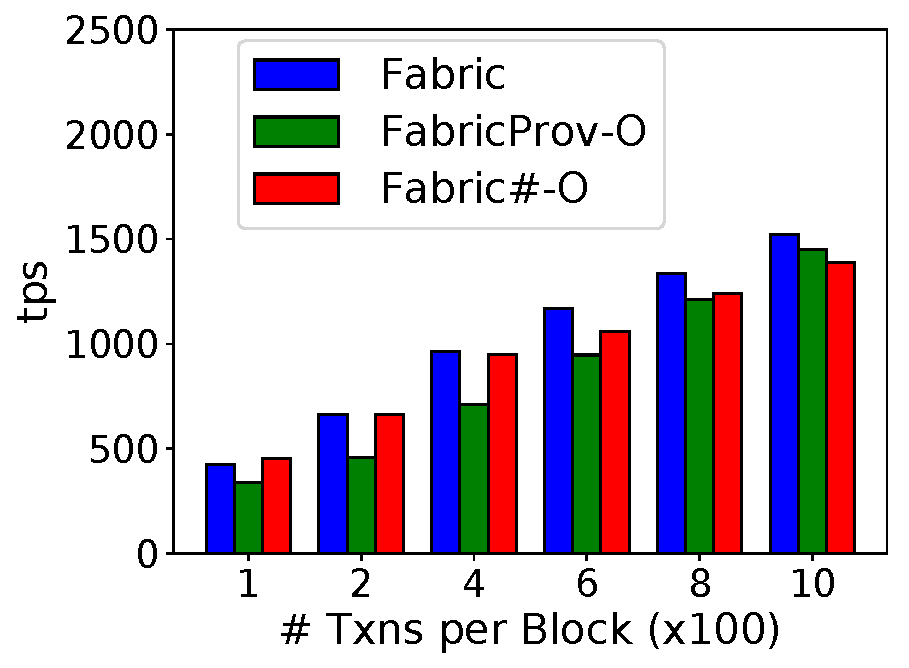
\includegraphics[width=0.99\textwidth]{chart/provenance/ycsb_thruput.pdf}
      \caption{YCSB}
      \label{chart:provenance:basic:ycsb}
    \end{subfigure}
    \begin{subfigure}{0.45\textwidth}
      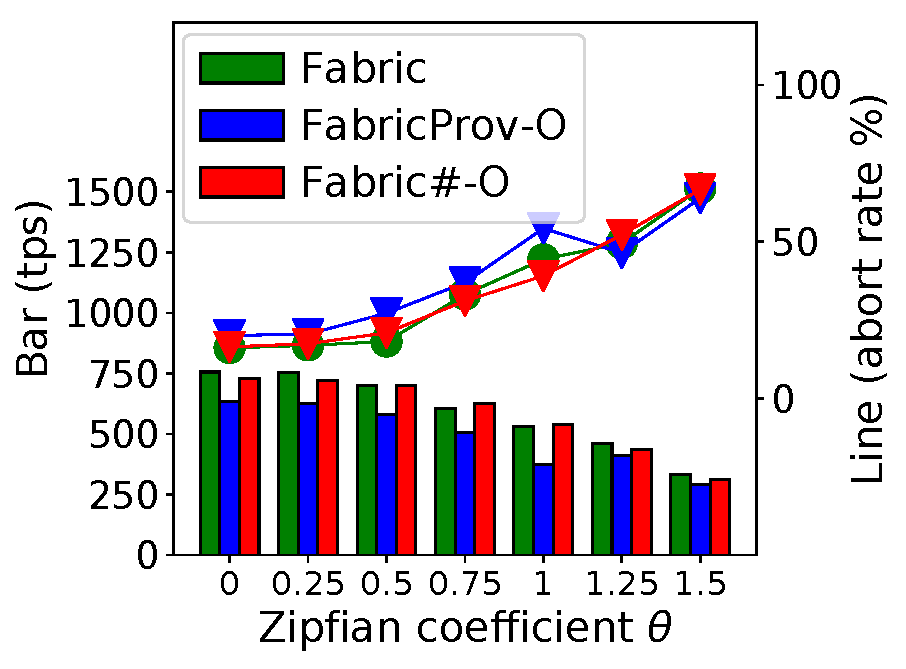
\includegraphics[width=0.99\textwidth]{chart/provenance/smallbank_skew.pdf}
      \caption{Smallbank (skewed)}
      \label{chart:provenance:basic:smallbank_skew}
    \end{subfigure}
    \caption{Effective throughput }
    % \subcaption*{ }
    \label{chart:provenance:basic}
\end{figure}

\subsection{Provenance Overhead and Utility}
\label{sec:provenance:exp:util}
\begin{figure}[tp]
	\centering
    \begin{subfigure}{0.45\textwidth}
      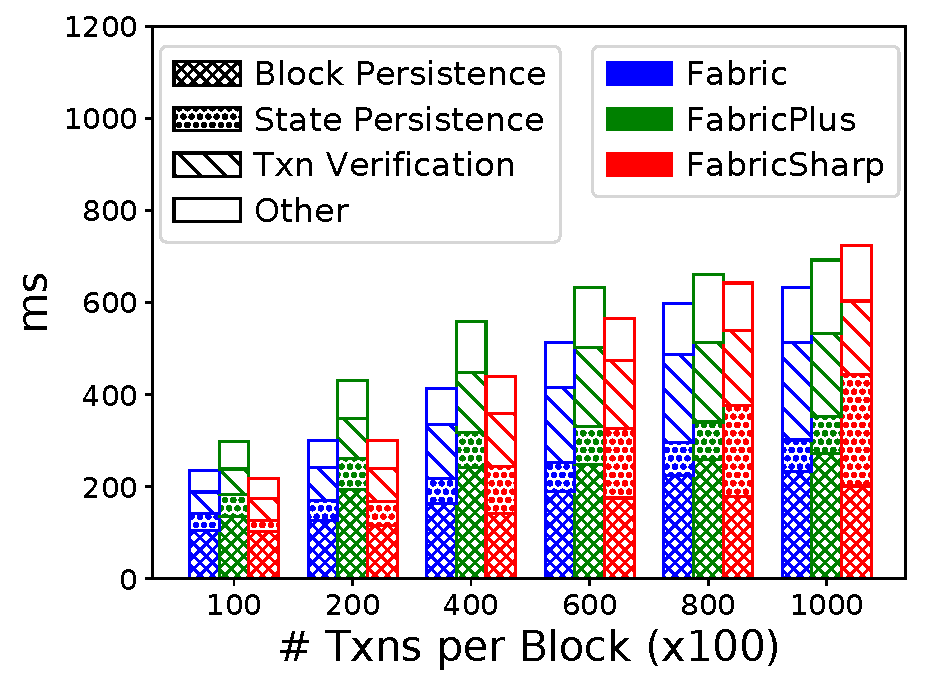
\includegraphics[width=0.99\textwidth]{chart/provenance/ycsb_breakdown.pdf}
      \caption{}
      \label{chart:provenance:ycsb_breakdown}
    \end{subfigure}
    \begin{subfigure}{0.45\textwidth}
      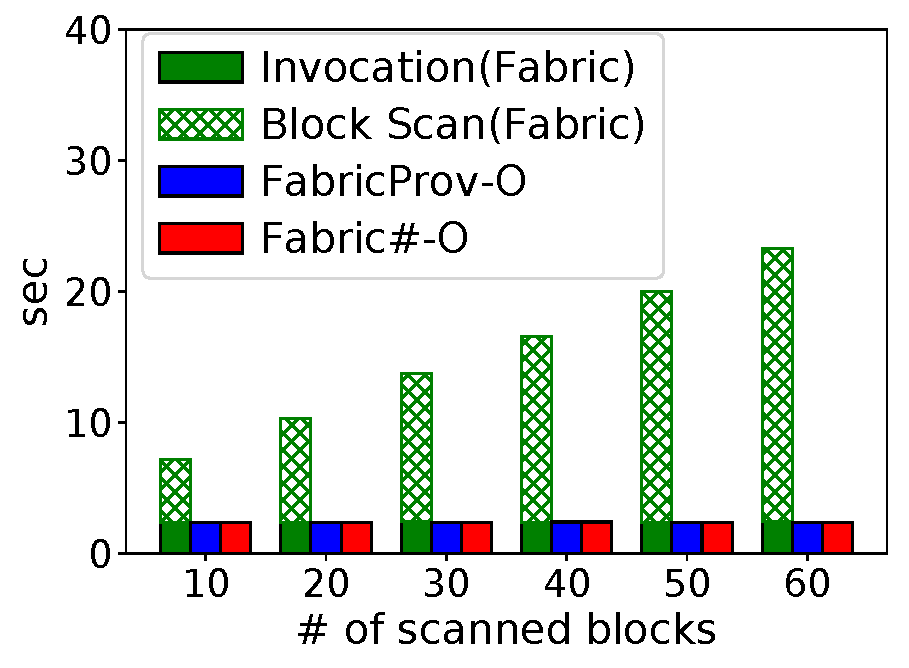
\includegraphics[width=0.99\textwidth]{chart/provenance/smallbank_util.pdf}
      \caption{}
      \label{chart:provenance:smallbank_util}
    \end{subfigure}
    \caption{Provenance overhead and utility }
    \subcaption*{(a) The breakdown of the block validation delay in YCSB (b) The delay to invoke the provenance-dependent \textit{Refund} logic in Smallbank.}
    % \label{chart:provenance:util_overhead}
\end{figure}
Figure~\ref{chart:provenance:ycsb_breakdown} breaks down the latency of block validation into multiple phases, block persistence, state persistence, transaction verification and others. 
As we have demonstrated in Chapter~\ref{sec:twin:exp:replication:model}, the sequential validation rate decides on the system capacity. 
Figure~\ref{chart:provenance:ycsb_breakdown} reveals a greater delay in {\fsPrO}, especially under small blocks. 
In particular, we observe that {\fsPrO} takes $25$\% more time to persist blocks than Fabric and {\fsO}.
By our careful inspection of the codebase, we realize that all Fabric variants construct an index on transactions when persisting a block. 
The index is persisted into the same storage (LevelDB) engine, which also maintains the latest state in Fabric.
However, that storage in {\fsPrO} incurs a heavier role: as explained in Chapter~\ref{sec:provenance:exp:setup}, it tracks all data provenance. 
The overloaded usage accounts for the increased delay to build the transaction index, which ultimately translates into the lower throughput in {\fsPrO}. 
On the other hand,  {\fsO} delegates the provenance tracking responsibility separately to ForkBase. 
It is why the block persistence in {\fsO} saves around $10$\% time compared with Fabric. 
However, {\fsO} takes more than 3 times to persist states (provenance) to ForkBase as Fabric and {\fsPrO} persist states (provenance) to LevelDB. 
For example with 1000 transactions per block, this delay in {\fsO} reports $242$ms while 69ms and 81ms in Fabric and {\fsPrO}.
This is understandable as {\fsO} additionally maintains the DASL and hash DAG for the provenance integrity. 
But fortunately, the delay ratio of the state persistence with respect to the overall block validation is small:
given the overall block validation delay is $723$ms in {\fsO}, this ratio is below $1/3$.
It explains why the total block validation delay in {\fsO} is within $14$\% and $4$\% more than Fabric and {\fsO}. 
So that {\fsO} reports the negligible performance overhead, even though it additionally preserves the provenance with the integrity guarantee.

The provenance-provided utility is abundant. In the Smallbank contract of {\fsPrO} and {\fsO}, we additionally encode a provenance-dependent code, which refunds an account with an amount computed from its recent transactions in latest blocks.
This is similar to the \texttt{Refund} example in Figure~\ref{code:prov:enhanced_contract}
Figure~\ref{chart:provenance:smallbank_util} compares the end-to-end invocation latency with Fabric, without the provenance support. 
The utility to expose smart contracts with provenance is tremendous. 
Both {\fsO} and {\fsPrO} are capable to consolidate the above provenance-dependent logic into a single invocation, which takes around 2s. 
In contrast, Fabric has to break the flow into two phases: first scan blocks for relevant transactions and then invoke the contract to perform the refund with the self-computed parameter. 
Worst still, the delay of the sequential block scanning increases with the number of requested recent blocks. 
Even though the block fetching can be done in parallel, 
the separation of two phases is not only error-prone but also security-flawed, as explained in Chapter~\ref{sec:provenance:intro}.

\subsection{Provenance Historical Query}
In the following experiments, we strip away the storage components from {\fsO} and {\fsPrO} for the specific analysis with the tailored workload. 

We first create 500 key-value tuples and then continuously issue update transactions until there are more 10k blocks in the ledger. We use 500 tuples, which is the same number of transactions in a block, so that every block contains a version of every tuple.  
We then execute a query for
the values of a key at different block numbers. Figure~\ref{chart:provenance:ycsb_dist_query} illustrates the query latency with  
increasing block distance from the last block. One can observe that when the distance is small, {\fsO} without DASL has the lowest latency. Without special index support for the query, it performs linear scan from the latest
version. Therefore, it is fast when the requested version is very recent because the number of read is small.
However, its performance degrades quickly as the distance increases. In particular, when the block distance
reaches $128$, the query is $4\times$ slower than {\fsO} with DASL. We observe that the query latency in
{\fsPrO} is independent of the block distance. It is because the query uses storage index directly. {\fsO}
outperforms the other two. Due to DASL, the query latency in {\fsO} is low when the block distance is
large. When the block distance increases, the latency in {\fsO} increases logarithmically, as opposed to
linearly without DASL.  

\begin{figure}[t]
	\centering
    \begin{subfigure}{0.3\textwidth}
      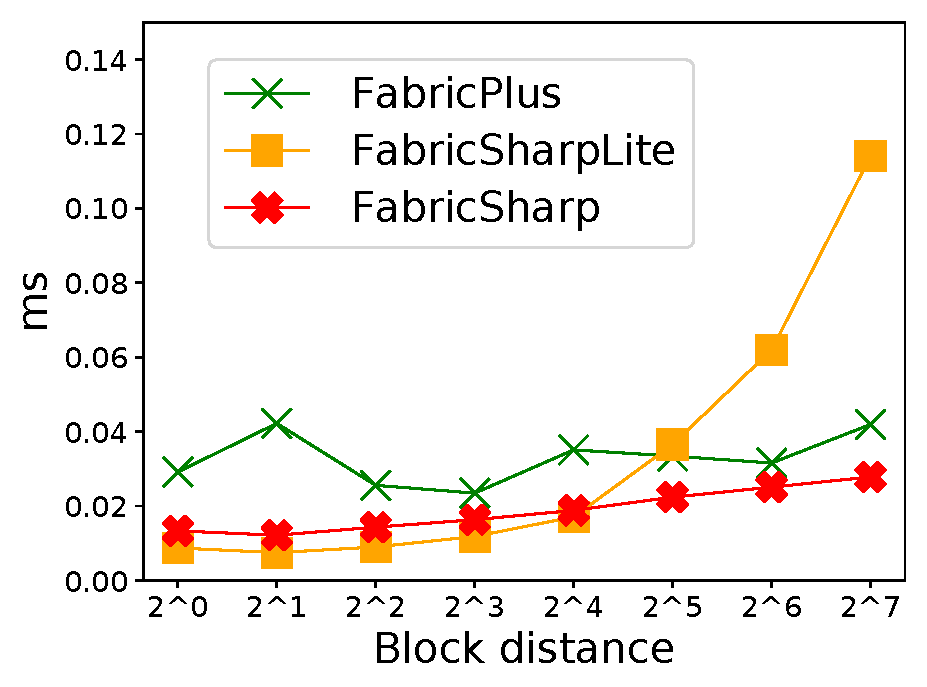
\includegraphics[width=0.99\textwidth]{chart/provenance/ycsb_dist_query.pdf}
      \caption{Version query I}
      \label{chart:provenance:ycsb_dist_query}
    \end{subfigure}
    \begin{subfigure}{0.3\textwidth}
      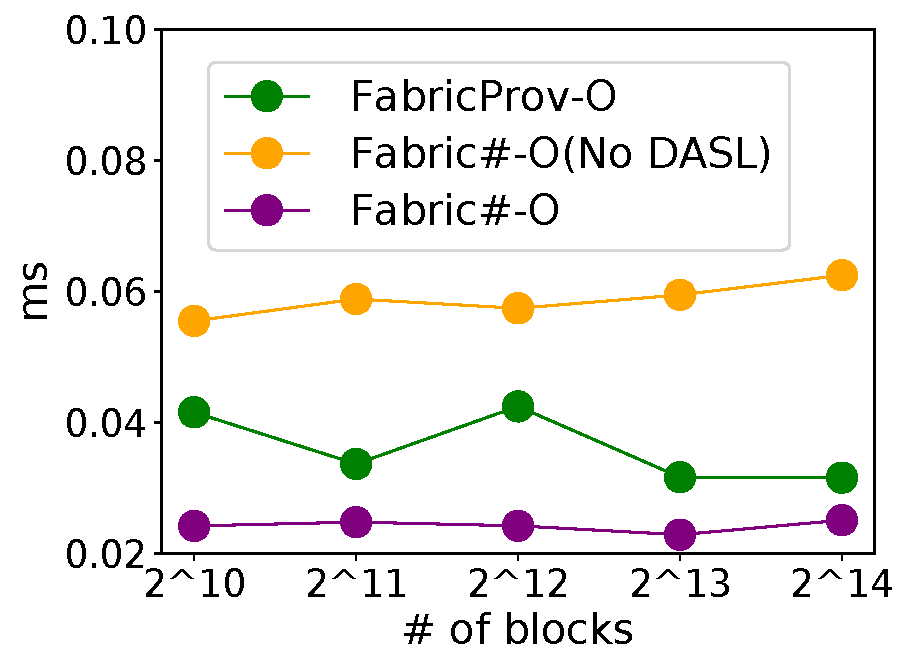
\includegraphics[width=0.99\textwidth]{chart/provenance/ycsb_blk_query.pdf}
      \caption{Version query II}
      \label{chart:provenance:ycsb_blk_query}
    \end{subfigure}
    \begin{subfigure}{0.3\textwidth}
      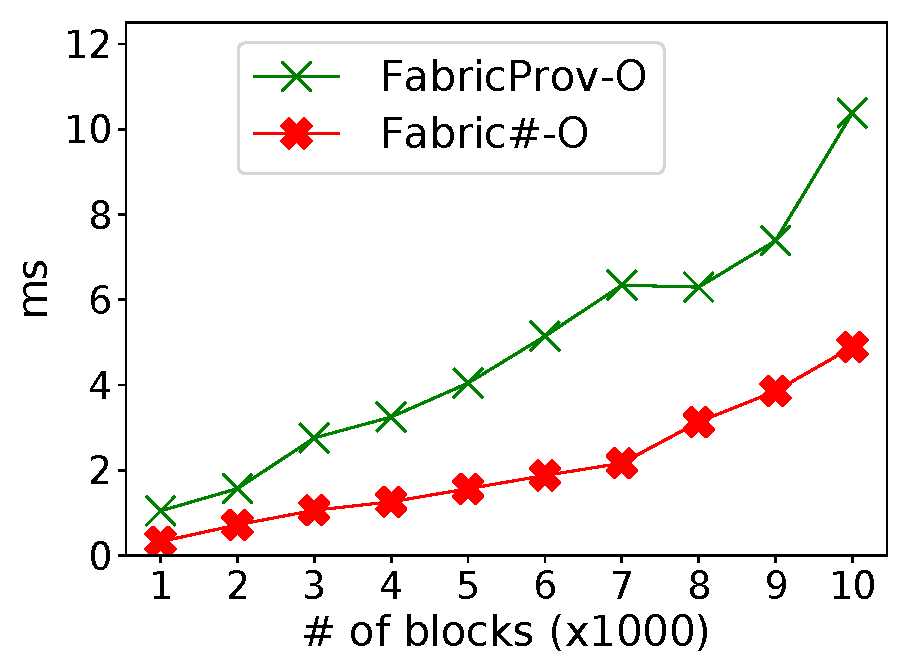
\includegraphics[width=0.99\textwidth]{chart/provenance/ycsb_version_scan.pdf}
      \caption{Version scan}
      \label{chart:provenance:ycsb_version_scan}
    \end{subfigure}
    \caption{Latency of historical queries}
    % \label{chart:provenance:util_overhead}
\end{figure}
We repeat the experiment above while fixing the block distance to $64$ and varying the total number of blocks.
Figure~\ref{chart:provenance:ycsb_blk_query} shows the results for the version query when the number of block increases.
It can be seen that the query latency in both {\fsO} with and without DASL remains roughly the same. In other words,
the performance of version queries in these systems are independent of the block numbers, which is due to the
DAG data model that tracks state versions. But the index reduces the
number of hops needed to be read. An interesting observation is that the latency of {\fsPrO} fluctuates
significantly. We attribute this fluctuation to the log-structure-merge tree index in the storage, in which the
requested version may reside at different levels of the tree when the total number of block increases. 

Next, we measure the latency for the operation that scan the entire version history of a given key.
Figure~\ref{chart:provenance:ycsb_version_scan} shows the scan latency with increasing number of blocks between {\fsPrO} and {\fsO}.  
For {\fsPrO}, we first construct the key range and rely on iterator for the scanning.  As the number of block
increases, the version history becomes longer which accounts for the linear increase in latency in both
systems.  However, {\fsO} outperforms {\fsPrO} by a constant factor. We attribute this difference to ForkBase's
optimizations for version tracking. 


\subsection{Provenance Dependency Query}
\begin{figure}[t]
	\centering
    \begin{subfigure}{0.68\textwidth}
      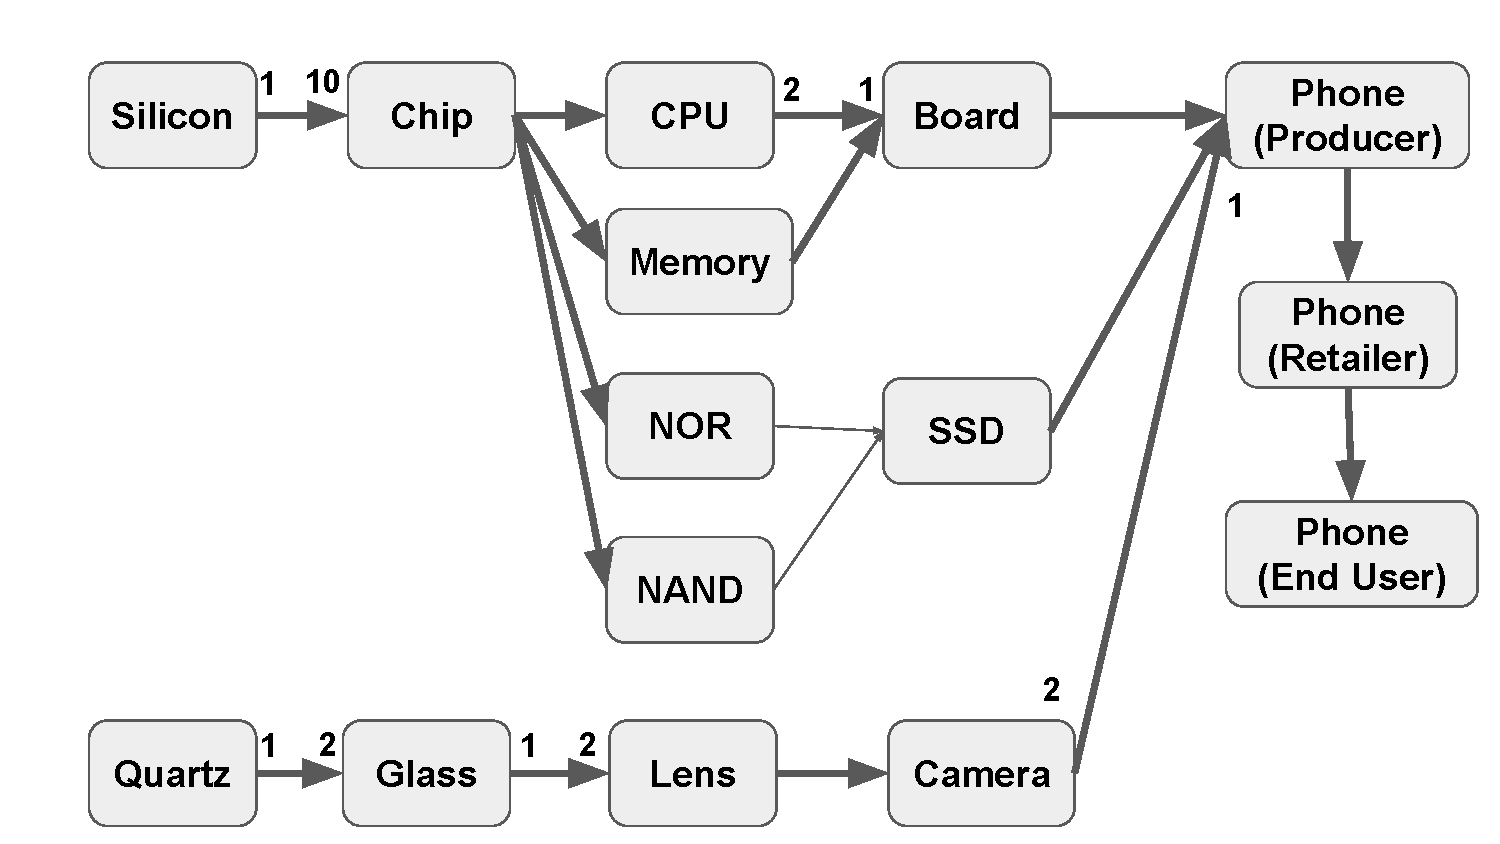
\includegraphics[width=0.99\textwidth]{diagram/provenance/supplychain.pdf}
      \caption{Dependency in the supply chain}
      \label{diagram:provenance:supply_chain_dag}
    \end{subfigure}
    \begin{subfigure}{0.45\textwidth}
      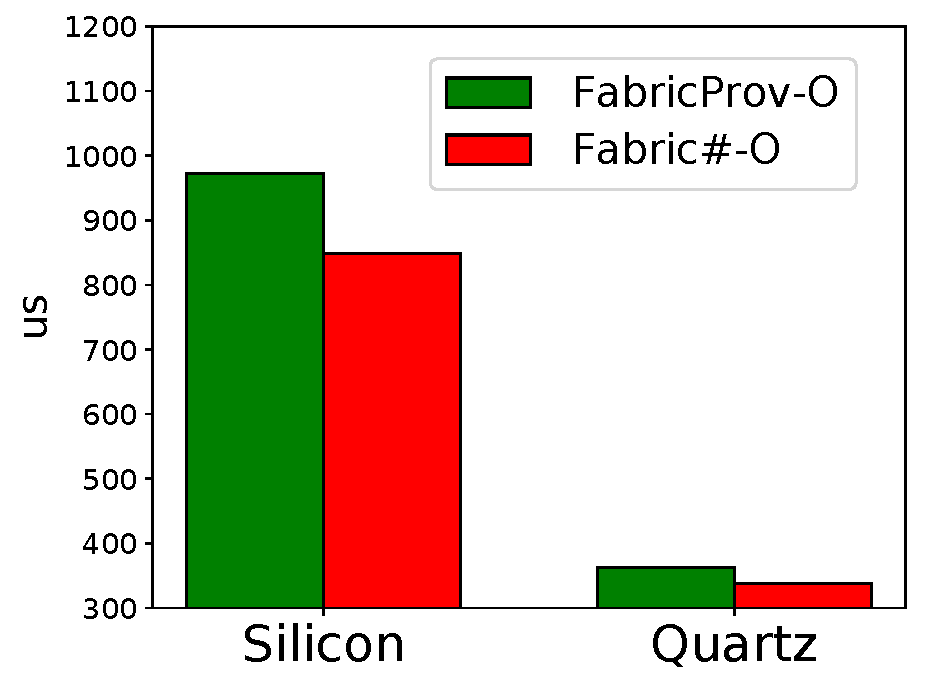
\includegraphics[width=0.99\textwidth]{chart/provenance/forward.pdf}
      \caption{Delay of forward query}
      \label{chart:provenance:supply_chain_forward}
    \end{subfigure}
    \begin{subfigure}{0.45\textwidth}
      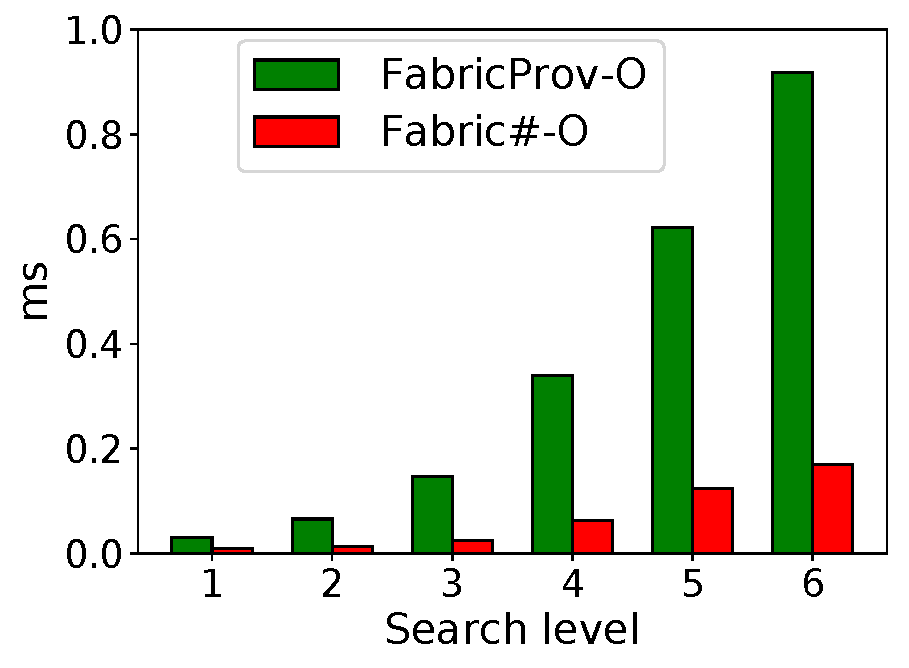
\includegraphics[width=0.99\textwidth]{chart/provenance/bfs.pdf}
      \caption{Delay of BFS traversal}
      \label{chart:provenance:supply_chain_bfs}
    \end{subfigure}
    \caption{Dependency queries on a simulated supply chain}
\end{figure}

For multi-state dependency tracking, we implement a contract for a supply chain
application shown in Figure~\ref{diagram:provenance:supply_chain_dag}.  In this application, a phone is assembled from intermediary
components which are made from other components or raw material. 
We pre-populate raw materials in both {\fsPrO} and {\fsO} and then issue transactions for the above transformation process. 
Each transaction consumes (reads) the source materials and generates (writes) new components. 
The steps after the phone production represent ownership changes from producers, retailers and end users.
This supply chain is more complex than the example in Figure~\ref{code:prov:contract}, as it consists of a DAG with
maximum depth of $6$. We generate synthetic data for this contract, and measure the latency of operations
using  \texttt{Forward} and \texttt{Backward} version tracking.

We evaluate the query performance with multi-state dependency. We populate the blockchain states with
raw materials and issue transactions that create new phones.  We perform two experiments. First, we assume
that one piece of silicon and quartz is found defected, and use forward tracking to find the
affected materials and phones. Second, we perform a standard DAG traversals, breadth-first search (BFS), to retrieve all the dependencies of a phone. 
Figure~\ref{chart:provenance:supply_chain_forward} compares the latency of forward tracking, and Figure
\ref{chart:provenance:supply_chain_bfs} shows the BFS traversal performance with varying depths.  For forward tracking, we observe that
{\fsO}'s delay is 10\% smaller than that of {\fsPrO}.  It takes less time to track the affected quartz than
the affected the silicon, because the silicon is at a deeper position in the supply
chain.  The gap between {\fsO} and {\fsPrO} is much more evident in the BFS traversal, 
in which the latencies of both systems grow exponentially with increasing depths.  However,
{\fsO} outperforms the baseline.  It is because the index in {\fsO} directly captures the dependencies,
whereas each backtrack operation in {\fsPrO} requires traversing the storage index.  As the number of queries
increases with the search depth, their performance gap accumulates.  

\subsection{Provenance Storage}
\begin{figure}[tp]
	\centering
    \begin{subfigure}{0.45\textwidth}
      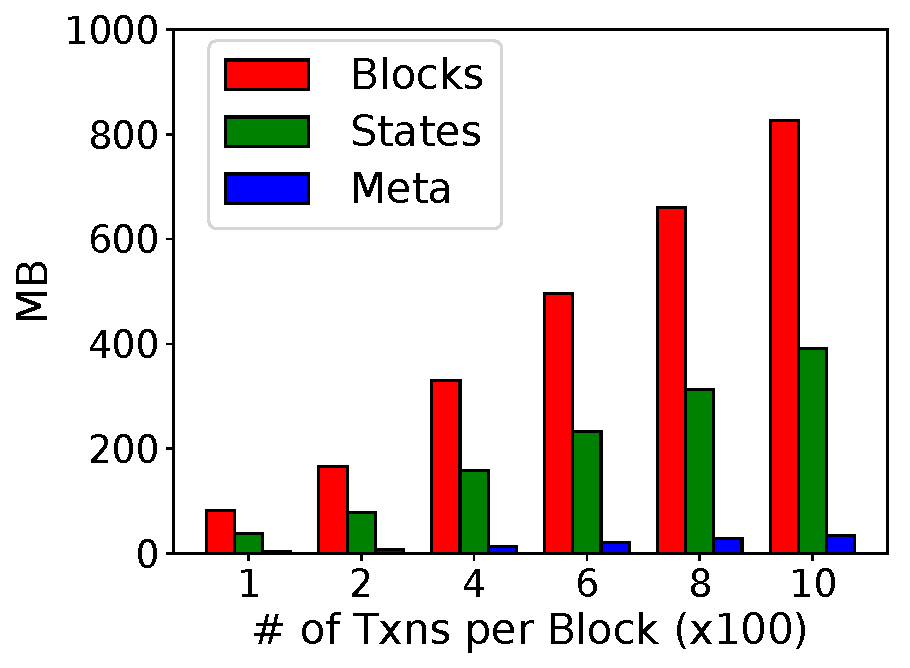
\includegraphics[width=0.99\textwidth]{chart/provenance/ycsb_blksize_storage.pdf}
      \caption{}
      \label{chart:provenance:ycsb_blksize_storage}
    \end{subfigure}
    \begin{subfigure}{0.45\textwidth}
      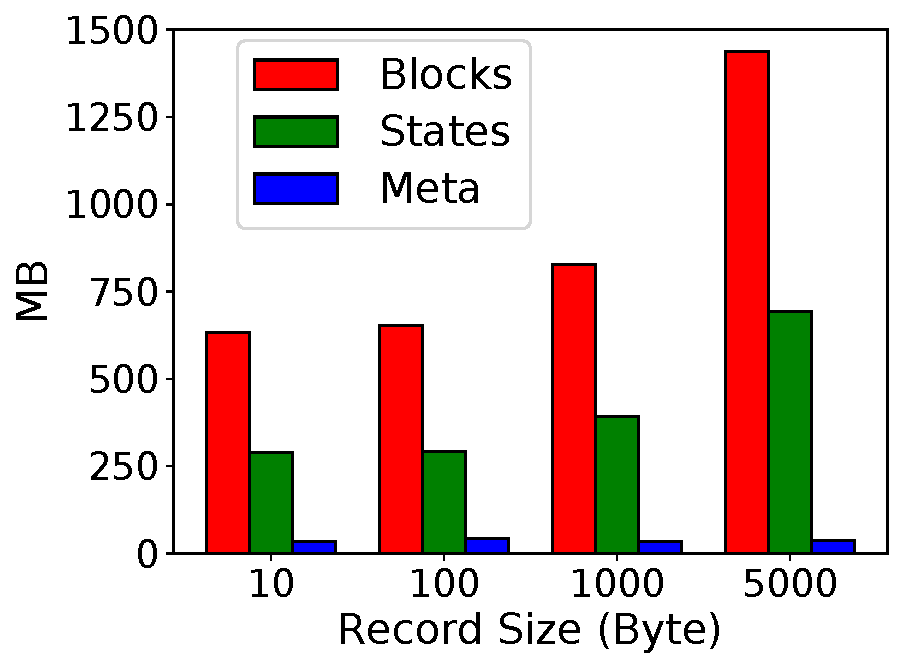
\includegraphics[width=0.99\textwidth]{chart/provenance/ycsb_recordsize_storage.pdf}
      \caption{}
      \label{chart:provenance:ycsb_recordsize_storage}
    \end{subfigure}
    \caption{Provenance storage size}
    \subcaption*{The storage space with (a) the varying block size and fixed record size (1000 bytes) (b) the varying record size and the fixed block size (1000 transactions per block). \textit{Meta} measures the size for all provenance information, such as hash pointers of Merkle DAG and DASL. }
    % \label{chart:provenance:util_overhead}
\end{figure}
In the last experiment, we populate 100 blocks with the YCSB workload. 
We place our focus solely on {\fsO} to understand the storage constitution for a blockchain application. 
Even though there might be differences if with {\fsPrO}, the differences are specific to their storages, that is, ForkBase in {\fsO} and LevelDB in{\fsPrO}. 
Their comparison is out of the scope of this thesis. 

We measure the consumed storage space with the varying block size and the record size, 
which are respectively reported in Figure~\ref{chart:provenance:ycsb_blksize_storage} and~\ref{chart:provenance:ycsb_recordsize_storage}. 
One can observe that the storage consumption grows linearly with the number of blocks. 
The storage increase is not evident until the record size grows to 5000 bytes. 
But the block content constantly accounts for the majority of the storage cost.
In particular, despite the different settings, blocks occupy around $66$\% of the entire space. 
The result further confirms the conclusion drawn in Chapter~\ref{sec:twin:exp:storage}: compared with the state storage, the ledger abstraction incurs the most storage overhead. 
But to our astonishment, we find that the storage consumption for data provenance is far less than expected, as shown in the negligible \texttt{Meta} bar. 
Their storage ratios are all below $1$\% when a block contains 1000 transactions. 
In the worst case with 100 transactions per block, the ratio is only $6.7$\%.
Hence we conclude that the storage overhead for the extra provenance and DASL index is insignificant. 

\chapter{A Transactional Perspective on \\Execute-order-validate Blockchains}
\label{ch:txn}
\section{Introduction}
\label{sec:txn:intro}
From Chapter~\ref{ch:twin}, blockchains systems can be classified into \textit{permissionless}
(\textit{public}), such as Bitcoin and Ethereum, and \textit{permissioned}
(\textit{private}), such as Hyperledger Fabric~\cite{androulaki2018hyperledger}.
%
In public blockchains, the data and transactional logic are transparent to the
public, hence, are subject to private data leakage.
%
Due to their openness, public blockchains use expensive PoW consensus.
%
This, together with the serial transaction execution limit these systems' capacity.
%
Addressing the limitations of public blockchains, Hyperledger Fabric is a
private blockchain that supports \emph{concurrent} transactions
\cite{androulaki2018hyperledger}.
%
A Fabric blockchain requires its members to enroll through a trusted membership service in order to interact with the blockchain.
In this chapter, we focus on permissioned blockchains as they are more suitable
for supporting applications such as supply-chain, healthcare and resource
sharing, and in particular, we use Fabric as the underlying blockchain system.

Fabric supports a new transaction execution architecture called
execute-order-validate (EOV).
%
In this architecture, a transaction's lifecycle consists of three phases, as detailed in~Chapter~\ref{sec:literature:execution:execute-order-validate}. In the
first phase, \textit{execution}, a client sends the transaction to a set of
nodes, or peers, specified by an endorsement policy.
%
The transaction is executed by these peers in parallel and its effects in terms
of read and written states are recorded.
%
Moreover, transactions from different clients may be parallelized during the
execution.
%
In the second phase, \textit{ordering}, a consensus protocol is used
to produce a totally ordered sequence of endorsed transactions grouped in
blocks.
%
This order is broadcast to all peers. In the third phase, \textit{validation},
each peer validates the state changes from the endorsed transactions with
respect to the endorsement policy and serializability. 
%
We will further elaborate the EOV architecture with an example in Chapter~\ref{sec:txn:background}. 

The new EOV architecture limits the execution details of a transaction to the
endorsing peers to enhance confidentiality and exploit concurrency. But such
concurrency comes at the cost of aborting transactions that do not abide
%
serializability.
%
We have quantified this cost with respect to the Smallbank workload in Figure~\ref{chart:intro:basic:smallbank_skew}.
%
Figure~\ref{chart:intro:basic:smallbank_skew} report both the raw and effective peak throughputs under the transaction workload with contention. 
%
In the latter, the Zipfian coefficient $\theta$ of the request distribution controls the contention. 
%
The raw throughput represents the in-ledger transaction rate, while the effective throughput represents committed transactions by excluding the aborted transactions from raw throughput. 
%
In Figure~\ref{chart:intro:basic:smallbank_skew}, a bar shows the raw throughput, while its blue part reports the effective throughput. 
%
As we can see with higher skewness, a substantial fraction of the in-ledger transactions are aborted for serializability. 
%
To be specific, this ratio grows to $67$\% when $\theta=1.5$, severely reducing the system processing volume. 

% \begin{figure}
%   \centering     
%   \includegraphics[width=0.8\textwidth]{chart/intro/skew.pdf}
%   \caption{Fabric's raw and effective throughput under both no-op transactions and single modification transactions with varying skewness}
%   \label{chart:txn:intro}
% \end{figure}

There are two notable directions attempting to address this limited volume. 
%
The first is to improve upon Fabric's architecture to enhance its
attainable throughput \cite{nasir2018performance, thakkar2018performance}.
%
For example, FastFabric proposes to split a node's functionality to alleviate the bottleneck and achieves the highest throughput among all improvements of Fabric~\cite{gorenflo2019fastfabric}. 
%
However, these approaches are implementation-specific and might not generalize well
to other blockchains.
%
The second direction is to abstract out the transaction lifecycle to reduce
abort rate.
%
For example, {\fabricPlusplus}~\cite{sharma2019blurring} uses
well-established concurrency techniques from databases to early abort
transactions or reorder them to reconcile the potential conflicts.




In this Chapter~\ref{ch:twin}, we propose a work corresponding to the second direction, as a major attempt to
\textit{databasify} blockchains.
%
In this proposal, we first take a principled approach to learn from transactional analysis
techniques in databases with optimistic concurrency control (OCC) and apply them
to enhance transaction processing in blockchains.
%
We formally analyze the behavior of the current implementations of Fabric, and discover that both
achieve \textit{Strong Serializability} \cite{bailis2013highly} (as described in Chapter~\ref{sec:txn:serializabilityAnalysis}).
%
In fact, these implementations are more stringent than
\textit{One-Copy Serializability} (or simply Serializability), as prescribed by the original Fabric protocol~\cite{androulaki2018hyperledger}.
%
Both systems employ a preventive approach which might over-abort transactions that are still serializable.
%
In contrast, our proposal consists of a novel reordering technique that
eliminates unnecessary abort due to in-ledger conflicts, with the serializability guarantee established on our theoretical insights. 
%
Our approach does not change Fabric's architecture, therefore it is orthogonal to the aforementioned optimizations, such as FastFabric \cite{gorenflo2019fastfabric}. 

In the following, Chapter~\ref{sec:txn:theory} expands the above analysis in full details. 
We will then draw out the plan to materialize it, and discuss the potential implementation challenges in Chapter~\ref{sec:txn:impl}.
At last, Chapter~\ref{sec:txn:exp} describes experiments for the evaluation.

% In summary, our paper makes the following contributions:
% % \begin{itemize}[leftmargin=1.8em]
% \begin{itemize}
% \item We theoretically analyze the resemblance of transaction processing in
%   blockchains with EOV architecture and databases with optimistic concurrency
%   control (Chapter~\ref{sec:txn:resembalance}).
%   %
%   Based on this resemblance, we analyze the transactional behavior of
%   state-of-the-art EOV blockchains, such as Fabric and {\fabricPlusplus}
%   (Chapter~\ref{sec:txn:serializabilityAnalysis}).
  
% \item We propose a novel theorem to identify transactions that can never be
%   reordered for serializability 
%   (Chapter~\ref{sec:txn:reorderabilityAnalysis}).
%   %
%   Based on this theorem, we propose efficient algorithms to early filter out
%   such transactions (Chapter~\ref{sec:txn:concurrencyControl}), 
%   with the serializability guarantee for the remaining after reordering.
%   We also discuss the security implications of our proposal (Chapter~\ref{sec:txn:securityanalysis}).
  

% \item We implement our proposed algorithms on top of {\fs} and extensively evaluate {\fs} by comparing it with the vanilla
%   Fabric, {\fabricPlusplus}(simulated by our baseline {\fsP}), and two other implementations based on database concurrency control techniques from one standard approach~\cite{CahillRF08} and a recent proposal by Ding et al~\cite{ding2018improving}.
%   %
%   The experimental results show that the remarkable speedup compared to the other systems.
%   %
% \end{itemize}

% The remaining of this paper is structured as follows.
% %
% Chapter~\ref{sec:txn:background} provides background on EOV blockchains and OCC techniques. 
% %
% Our theoretical analysis follows in Chapter~\ref{sec:txn:theory}, ending with our
% reordering algorithm.
% %
% Chapter~\ref{sec:txn:impl} describes the implementation of our approach.
% %
% Chapter~\ref{sec:txn:exp} reports our experimental results.

\section{Background}
\label{sec:txn:background}
\begin{figure*}[h!]
    \begin{subfigure}{0.71\textwidth}
      \centering
      \includegraphics[width=0.99\textwidth]{diagram/txn/background.pdf}
      % \caption{Workflow of Hyperledger Fabric with example transactions}
      \caption{}
      \label{diagram:txn:background_fabric}
    \end{subfigure}
    \begin{subfigure}{0.28\textwidth}
      \centering
      \includegraphics[width=0.75\textwidth]{diagram/txn/fabric_orderer.pdf}
      \caption{}
      % \caption{Procedures in Fabric Orderer}
      \label{diagram:txn:background_orderer}
    \end{subfigure}
    \caption{Background in Execute-order-validate architecture and {\fabricPlusplus}'s instrumentation}
    \subcaption*{(a) Example of transaction workflow in Fabric. An arrow represents the lifespan of a transaction's execution (simulation), e.g, Txn1 starts its execution immediately after block 1 and finishs its simulation after block 2. (b) Procedures replicated in each Fabric Orderer.
    {\fabricPlusplus} introduces a reordering step before the block formation to reduce the transaction abort rate.}
    \label{diagram:txn:background}
\end{figure*}

\subsection{EOV~architecture~in~Fabric~and~{\fabricPlusplus}}
\label{sec:txn:background_fabric}

Hyperledger Fabric~\cite{androulaki2018hyperledger} is a state-of-the-art
permissioned blockchain that features a modular design based on the EOV architecture.
% (execute-order-validate)
%
{\fabricPlusplus}~\cite{sharma2019blurring} is an optimization of Fabric, which reorders transactions after consensus to reduce the abort rate.
%
A Fabric/{\fabricPlusplus} blockchain is run by a set of authenticated nodes, whose identity is
provided by a membership service.
%
A node in this blockchain has one of the following three roles:
%
(i) \textit{client} which submits a transaction proposal for execution,
%
(ii) \textit{peer} which \textit{executes} and \textit{validates}
transaction proposals,
%
or (iii) \textit{orderer} which \textit{orders} transactions and batches
them in blocks.
%
Transaction order is determined collectively by all orderers in
the blockchain based on a consensus protocol.
%
% Orderers are responsible for block formation.

The state of a blockchain after forming a block is maintained by a
versioned key-value store.
% 
Each entry in this store is a tuple (\texttt{key}, \texttt{ver},
\texttt{val}), where \texttt{key} is a unique name representing the entry, and
\texttt{ver} and \texttt{val} are the entry's latest version and value, respectively.
% 
Moreover, \texttt{ver} is a pair consisting of the sequence number of the block
and the transaction that updated the entry.
%
For example, in Figure~\ref{diagram:txn:background_fabric}, the entry \entry{C}{2,1}{201} in
the state after block $2$ indicates that the key \texttt{C} contains the latest
value $201$ which was lastly updated by the 1st transaction in block $2$.

\begin{table}[tp]
\centering
\caption{The transaction summary in Figure~\ref{diagram:txn:background}.}
\label{txn:tab:simulation}
\small
\setlength\tabcolsep{2.3pt}
\begin{tabular}{|c|c|cc|cc|c|l|c|l|c|l|}
\hline
\multicolumn{2}{|c|}{}
& \multicolumn{2}{c|}{\textbf{Txn1}}
& \multicolumn{2}{c|}{\textbf{Txn2}}
& \multicolumn{2}{c|}{\textbf{Txn3}}
& \multicolumn{2}{c|}{\textbf{Txn4}}
& \multicolumn{2}{c|}{\textbf{Txn5}}
\\

\hline

\multirow{2}{*}{\textbf{Readset}} & Key
& B & C
& A & {\color{red} \textbf{B}}
& \multicolumn{2}{c|}{B}
& \multicolumn{2}{c|}{{\color{red} \textbf{C}}}
& \multicolumn{2}{c|}{{\color{red} \textbf{C}}}
\\

& Version
& 1,2 & 2,1
& 1,1 & {\color{red} \textbf{1,2}}
& \multicolumn{2}{c|}{2,1}
& \multicolumn{2}{c|}{{\color{red} \textbf{2,1}}}
& \multicolumn{2}{c|}{{\color{red} \textbf{2,1}}}
\\

\hline

\multirow{2}{*}{\textbf{Writeset}} & Key
& \multicolumn{2}{c|}{C}
& \multicolumn{2}{c|}{C}
& \multicolumn{2}{c|}{{\color{blue} \textbf{C}}}
& \multicolumn{2}{c|}{B}
& \multicolumn{2}{c|}{A}
\\

& Value
& \multicolumn{2}{c|}{301}
& \multicolumn{2}{c|}{302}
& \multicolumn{2}{c|}{{\color{blue} \textbf{303}}}
& \multicolumn{2}{c|}{304}
& \multicolumn{2}{c|}{305}
\\

\hline

\multirow{2}{*}{\textbf{Commit status}} & Fabric
& \multicolumn{2}{c|}{\textbf{N.A.}}
& \multicolumn{2}{c|}{\xmark}
& \multicolumn{2}{c|}{\vmark}
& \multicolumn{2}{c|}{\xmark}
& \multicolumn{2}{c|}{\xmark}
\\

& {\fabricPlusplus}
& \multicolumn{2}{c|}{{\xmark}}
& \multicolumn{2}{c|}{{\xmark}}
& \multicolumn{2}{c|}{{\xmark}}
& \multicolumn{2}{c|}{\vmark}
& \multicolumn{2}{c|}{\vmark}
\\

\hline
\end{tabular}
\subcaption*{
  Staled reads and installed writes are
  marked in {\color{red} red} and {\color{blue} blue} colors. The symbols {\vmark}, {\xmark}, \textbf{N.A.} respectively indicate committed, aborted, or not-allowed transactions.}
\end{table}


In Fabric/{\fabricPlusplus}, the workflow of a transaction consists of three phases:
execution, ordering, and validation.
%
We elaborate on these phases below, using the example in
Figure~\ref{diagram:txn:background_fabric}.

\textbf{Execution}. In this phase, clients propose transactions
  consisting of smart contract invocations to a set of endorsing peers,
  which are selected by an endorsement policy.
  %
  Each endorsing peer executes transaction proposals concurrently and
  speculatively and returns the simulation results together with its endorsement
  signature.
  % 
  The results contain two value sets called the \textit{readset} and the
  \textit{writeset} which respectively represent the version dependencies (all
  keys read along with their version numbers) and the state updates (all keys
  modified along with their new values) produced by the simulation.
  %
  For example, the readset and writeset of transactions in
  Figure~\ref{diagram:txn:background_fabric} are summarized in Table~\ref{txn:tab:simulation}.
  % 
  Throughout the execution, a transaction holds a read lock on the
  state database to guarantee that read values are the latest.
  %
  Transactions that read across blocks, such as \texttt{Txn1} in
  Figure~\ref{diagram:txn:background_fabric}, are not allowed in Fabric.
  %
  In contrast, {\fabricPlusplus} optimistically removes this lock for more parallelism but aborts transactions that read across blocks.
  %
  After a client collects enough identical simulation results as required
  by the endorsement policy, it packages them into a single transaction and
  submits it to orderers.
  % %
  % \trung{To Pingcheng: I feel that the last two sentences are confusing. Can we
  %   drop them?} \rpc{They are fine here.} \dumi{They indeed break the flow.}

% \item 
\textbf{Ordering}. In this second phase, orderers receive
  transactions and sequence them into a total order to form a block, 
  as shown in Figure~\ref{diagram:txn:background_orderer}.
  %
  Each orderer may belong to different administrative domains and receive different transaction proposals from various clients. 
  %
  But all orderers rely on a single consensus protocol to establish a common transaction order.
  % 
  Fabric/{\fabricPlusplus} outsources this consensus service to Kafka. 
  %
  With the consistent transaction stream from the consensus, each orderer employs the same block formation protocol to batch transactions into blocks, and consequently delivers them to peers.  
  % 
  A block is formed when the number of pending transactions reach the threshold or a timeout triggers. 
  %
  For example, in Figure~\ref{diagram:txn:background_fabric}, Orderer1 receives \texttt{Txn5} and Orderer2 receives \texttt{Txn2},  \texttt{Txn3}, and \texttt{Txn4}. 
  %
  They send the transactions to the consensus service and receive the same transaction order. 
  %
  Based on this order, both orderers package the transactions into identical blocks, i.e., block 3 with  \texttt{Txn2} to  \texttt{Txn5}, given that the protocol limits the maximum number of transactions per block to 4. 
  

% \item 
\textbf{Validation}. This phase is executed by each peer after
  a block has been retrieved from orderers.
  %
  Transactions in a block are sequentially validated based on the
  corresponding endorsement policy and transaction serializability.
  %
  The serializability of a transaction is tested by inspecting the
  staleness of its readset. The transaction is marked as invalid if it
  reads a key whose version at the read time is inconsistent (or older) than the
  latest version.
  %
  For example, in Figure~\ref{diagram:txn:background_fabric}, transaction \texttt{Txn2} in
  block $2$ is unserializable since it reads key \texttt{B} with version
  $(1,2)$ from block $1$, which is inconsistent with the latest version $(2,1)$
  in block $2$.
  %
  Suppose that \texttt{Txn3} passes the serializability test and updates the version of key \texttt{C} from $(2,1)$ to $(3,3)$ in block $3$. Then, transactions \texttt{Txn4} and \texttt{Txn5} become invalid, since they both read an inconsistent version of key \texttt{C} in block $2$.
  %
  Hence, after this validation phase, only transaction \texttt{Txn3} in
  block $3$ is committed, while transactions \texttt{Txn2}, \texttt{Txn4}, \texttt{Txn5} are aborted.
  %
  To satisfy the serializability constraint, {\fabricPlusplus} introduces a reordering step immediately before block formation but after consensus.
  % 
  The reordering is based on the commit order determined by the consensus and the accessed records in the transactions. 
  % 
  For example, each orderer in {\fabricPlusplus} puts \texttt{Txn3} behind \texttt{Txn4} and  \texttt{Txn5}. Then, \texttt{Txn4} and \texttt{Txn5} are committed while \texttt{Txn3} is aborted. 
  % 
  Hence, {\fabricPlusplus} commits one more transaction than Fabric. 
  
\subsection{Optimistic Concurrency Control in Databases}
Unlike pessimistic concurrency control, the OCC technique does not hold locks to
regulate transactional interference.
%
Instead, each transaction has a unique \textit{start timestamp} assigned to it
from a global atomic clock.
%
All queries reflect the state snapshot of the database at the start timestamp,
without observing later changes.
%
Each transaction is also assigned an {\textit{end timestamp}}. 
%
Before committing, the database system checks the validity of a transaction
based on these two timestamps and the accessed records.
%
OCC can easily achieve \textit{Snapshot Isolation}, which disallows concurrent
transactions updating the same key~\cite{berenson1995critique}.
%
Considering the fact that Snapshot Isolation suffers anomalies such as
Lost Update and Write Skew, a number of attempts have been
made to transform Snapshot Isolation to Serializable level
\cite{fekete2005making, yabandeh2012critique, bornea2011one}.

\section{Theoretical Analysis}
\label{sec:txn:theory}

In this section, we first describe the resemblance of transaction processing
techniques in EOV blockchains and OCC databases.
%
Then, we use the transactional analysis method of OCC databases to
reason about the serializability behavior of EOV blockchains, such as Fabric and {\fabricPlusplus}.
%
Finally, we propose a reordering-based concurrency control algorithm for ordering
serializable transactions in EOV blockchains, 
along with the discussion on its security implications.

\subsection{Resemblance~in~Transaction~Processing}
\label{sec:txn:resembalance}
%
Similar to database systems where the concept \textit{database snapshot} is used
to describe a read-only, static view of a database~\cite{kung1981optimistic}, in blockchains, we can define the similar concept of \textit{blockchain snapshot} as follows.

\begin{definition}[Blockchain snapshot]
  \label{defn:snapshot}
  A blockchain snapshot is the state of a blockchain after a block is committed.
  %
  Let $M$ be the sequence number of the committed block, then the
  corresponding snapshot is denoted as $M$ and is said to have the sequence
  number $(M{+}1,0)$~\footnote{We use the two-value tuple with 0 fixed for the
    second element. This is to facilitate the ordering relations $<$ of sequence numbers of blockchain snapshots and
    transaction timestamps.}.
\end{definition}

\begin{definition}[Snapshot consistency]
  \label{defn:inconsistentExe}
  A transaction is snapshot consistent if there exists a blockchain snapshot M
  from which all the transaction's records are read.
\end{definition}

Transactions in Fabric satisfy snapshot consistency since Fabric uses a lock to
ensure the simulation is done against the latest state.
%
{\fabricPlusplus} optimistically removes the lock but early aborts transactions which read across blocks.
%
Hence, it also satisfies the snapshot consistency. 
%
However, eliminating transactions based on cross-block reading might
lead to over-aborting snapshot consistent transactions.

\begin{example}
  \label{example:txn:acrossBlk}
  In Figure~\ref{diagram:txn:theory_snapshot}, \texttt{Txn1} reads key
  \texttt{A} of version $(1,1)$ in snapshot $1$ and key \texttt{B} of
  version $(2,1)$ in snapshot $2$.
  %
  These versions are the same as the versions of keys \texttt{A} and \texttt{B} in snapshot $2$.
  %
  Hence, \texttt{Txn1} is \textit{snapshot consistent} with block snapshot $2$.
  %
  In contrast, transaction \texttt{Txn2}, which also reads across blocks, does
  not achieve snapshot consistency because the value of previously read key B
  changes in block 2.
  %
  % \texttt{Txn2}, unlike \texttt{Txn1}, is correctly aborted by \heur{H1}.
\end{example}


\begin{figure*}[tp] \centering
  \begin{subfigure}{0.7\textwidth}
    \includegraphics[width=0.99\textwidth]{diagram/txn/theory_snapshot.pdf}
    \caption{Txn1, which reads across blocks, is snapshot consistent and can be
    scheduled with serializability. Txn2 is not as its early-read key B
    is updated before its execution ends.}
    \label{diagram:txn:theory_snapshot}
  \end{subfigure}\hfill
  \begin{subfigure}{0.27\textwidth}
    \includegraphics[width=0.99\textwidth]{diagram/txn/theory_notation.pdf}
    \caption{Concise notation to represent a transaction}
    \label{diagram:txn:theory_notation}
  \end{subfigure}
  \caption{An example of transactions reading across blocks}
  % \label{fig:theory_inconsistent}
\end{figure*}

\begin{proposition}
  \label{proposition:crossblockRead}
  There exist snapshot-consistent transactions that read across blocks. For such
  a transaction, its block snapshot is determined by its last read operation.
\end{proposition}

\begin{proof}
  \texttt{Txn1} in Figure~\ref{diagram:txn:theory_snapshot} is a witness example.
  %
  We have described in Example~\ref{example:txn:acrossBlk} that \texttt{Txn1} reads across
  blocks 1 and 2, and it is still consistent with block snapshot 2.
\end{proof}

Proposition~\ref{proposition:crossblockRead} shows that a legitimate transaction in an
EOV blockchain can read across blocks, if their states are consistent.
%
This makes the EOV blockchain similar to an OCC database, as the
latter also reads from consistent states determined by the transaction's start
timestamp.
%
We also observe that the blockchain's sequence numbers have similar properties with
databases' timestamps, such as atomicity, monotony, total order, and
unique mapping to snapshots.
%
Therefore, we define the timestamps of blockchain transactions using their
sequence numbers.

\begin{definition}[Start timestamp]
  \label{defn:start-timestamp}
  The start timestamp of transaction \texttt{Txn}, denoted by \startTS{Txn}, is
  the sequence number of its read snapshot.
\end{definition}

\begin{definition}[End timestamp]
  \label{defn:commit-timestamp}
  The end timestamp of transaction \texttt{Txn}, denoted by \commitTS{Txn}, is its sequence number in the block, determined by the consensus. 
\end{definition}

For example, in Figure~\ref{diagram:txn:theory_snapshot}, \texttt{Txn1} has $\startTS{Txn1} =
(3, 0)$ and $\commitTS{Txn1} = (3,1)$, since it lastly reads from block $2$ and
occupies the first position in block $3$.
%
For brevity, in later paragraphs, we use the notation presented in
Figure~\ref{diagram:txn:theory_notation} to denote a transaction.
%
Moreover, the sequence numbers of transactions' start or end timestamps are lexicographically ordered, e.g., (2,1) < (2,2) = (2,2) < (3,0).

\begin{definition}[Concurrent transactions]
  \label{defn:concurrent-transaction}
  Two transactions \texttt{Txn1} and \texttt{Txn2} are said to be concurrent if their executions overlap. 
  To be specific, if \texttt{Txn1} ends earlier than \texttt{Txn2} (i.e., $\commitTS{Txn1}$ < $\commitTS{Txn2}$), then \texttt{Txn2} must start before \texttt{Txn1} ends (i.e., $\startTS{Txn2}$ < $\commitTS{Txn1}$). Otherwise, if \texttt{Txn2} ends earlier than \texttt{Txn1} (i.e., $\commitTS{Txn2}$ < $\commitTS{Txn1}$), then \texttt{Txn1} must start before \texttt{Txn2} ends (i.e., $\startTS{Txn1}$ < $\commitTS{Txn2}$).
\end{definition}

\begin{proposition}
  \label{proposition:concurrency}  
  Each pair of transactions in the same block are concurrent. 
\end{proposition} 

\begin{proof}
  Suppose two transactions \texttt{Txn1} and \texttt{Txn2} are committed in the
  same block $M$ at position $p$ and $q$, respectively, where $p < q$.
  %
  Since the latest block that \texttt{Txn2} can read from is $M{-}1$, we have
  that: $\startTS{Txn2} \le (M,0) < \commitTS{Txn1} = (M,p) < \commitTS{Txn2} =
  (M,q)$.
  %
  Hence, \texttt{Txn1} and \texttt{Txn2} are concurrent.
\end{proof}

\begin{proposition}
  \label{proposition:nonconcurrency}  
  The reverse of Proposition~\ref{proposition:concurrency} is not true: there are concurrent transactions not belonging to the same block.
\end{proposition} 

\begin{proof}
  We present a witness example in Figure~\ref{diagram:txn:theory_concurrency}, where
  transactions \texttt{Txn1} and \texttt{Txn2} respectively belong to block $M$
  and $M{+}1$. However, \texttt{Txn2} reads from a block earlier than $M$.
  %
  Hence, we have: $\startTS{Txn2} \le (M,0) < \commitTS{Txn1} = (M,1) <
  \commitTS{Txn2} = (M{+}1,1)$.
  %
  Therefore, \texttt{Txn1} and \texttt{Txn2} are concurrent.
\end{proof}

\begin{figure}[tp] \centering
  \includegraphics[width=0.85\textwidth]{diagram/txn/theory_concurrency.pdf}
  \caption{Concurrency of transactions within and across blocks}
  \subcaption*{\texttt{Txn2} and \texttt{Txn3} are in the same block and concurrent. \texttt{Txn1} and \texttt{Txn2} are in different blocks, but they are still concurrent. \texttt{Txn1} and \texttt{Txn3} are not concurrent.}
  \label{diagram:txn:theory_concurrency}
\end{figure}

From the above two propositions, concurrency does not only occur between transactions within the same block.  
%
{\fabricPlusplus} fails to consider dependencies among transactions across blocks.
%
Hence, its reordering effect is limited. 


\subsection{Serializability Analysis}
\label{sec:txn:serializabilityAnalysis}

\begin{figure*}
  \centering
  \begin{subfigure}{0.45\textwidth}
      \includegraphics[width=0.99\textwidth]{diagram/txn/dependency/theory_noncurrent_ww.pdf} 
      \caption{\textit{n-ww}}
  \end{subfigure}
  \begin{subfigure}{0.45\textwidth}
      \includegraphics[width=0.99\textwidth]{diagram/txn/dependency/theory_noncurrent_wr.pdf}
      \caption{\textit{n-wr}}
  \end{subfigure}
  \begin{subfigure}{0.45\textwidth}
      \includegraphics[width=0.99\textwidth]{diagram/txn/dependency/theory_noncurrent_rw.pdf} 
      \caption{\textit{n-rw}}
  \end{subfigure}
  \begin{subfigure}{0.45\textwidth}
      \includegraphics[width=0.99\textwidth]{diagram/txn/dependency/theory_concurrent_ww.pdf} 
      \caption{\textit{c-ww}}
  \end{subfigure}
  \begin{subfigure}{0.45\textwidth}
      \includegraphics[width=0.99\textwidth]{diagram/txn/dependency/theory_concurrent_rw.pdf} 
      \caption{\textit{c-rw}}
  \end{subfigure}
  \begin{subfigure}{0.45\textwidth}
      \includegraphics[width=0.99\textwidth]{diagram/txn/dependency/theory_concurrent_antirw.pdf} 
      \caption{\textit{anti-rw}}
  \end{subfigure}  
  \caption{Six canonical dependencies between snapshot transactions.}
  \subcaption*{(a), (b), and (c) are non-concurrent and (d), (e), and (f) are concurrent.}
  \label{diagram:txn:theory_dependencies}
\end{figure*}

Figure~\ref{diagram:txn:theory_dependencies} shows all six scenarios of canonical transaction dependency (or conflict) between snapshot transactions, as described by
\cite{fekete2005making}.
%
Among them, three dependencies, namely \scenario{n-ww}, \scenario{n-wr}, and
\scenario{n-rw} are between non-concurrent transactions.
%
The other three dependencies, namely \scenario{c-ww}, \scenario{c-rw}, and \scenario{anti-rw} are between concurrent transactions.
%
According to the conflict serializability theorem in
\cite{weikum2001transactional}, the effect of a serializable transaction
schedule is equivalent to any serialized transaction history that respects
dependency order.
%
Note that the dependency graph of the serializable transaction schedule must be acyclic.

\begin{definition}[Strong Serializability]
  A schedule of transactions is \textit{Strong Serializable} if its effect is
  equivalent to the serialized history, which conforms to the transactions'
  commit order determined by their end timestamps.
\end{definition}

\begin{theorem}   
  \label{theory:strict}
  A schedule of transactions without \scenario{anti-rw} achieves Strong Serializability.
\end{theorem}

\begin{proof}
  We first prove that any transaction schedule without \scenario{anti-rw} achieves Serializability.
  %
  By contradiction, suppose that such a transaction schedule does not achieve Serializability.
  %
  Then, in the schedule there must be a subset of transactions with a dependency cycle,
  in which the last committed transaction is denoted by \texttt{Txn}.
  %
  Then \texttt{Txn} must exhibit an \scenario{anti-rw} dependency because
  \scenario{anti-rw} is the only one among all six dependencies that relates
  later transactions to earlier ones.
  %
  But this contradicts our assumption. 
  %
  Hence, the transaction schedule is serializable.
  %
  Next, we prove that it also achieves Strong Serializability.
  %
  Since the order of the five remaining dependencies is consistent to their
  commit order, the serialized history that respects the commit order also
  respects the dependency order.
  %
  According to the conflict serializability theorem in
  \cite{weikum2001transactional}, this serialized transaction history has the
  equivalent effect of the serializable schedule.
  %
  Hence, the transaction schedule is Strong Serializable.
\end{proof} 

We remark that Fabric/{\fabricPlusplus} do not allow \scenario{anti-rw} between two transactions because the latter transaction would read an old version of the updated key, hence, it must be aborted.
Based on Theorem~\ref{theory:strict}, transactions in Fabric/{\fabricPlusplus} satisfy Strong Serializability, which is more stringent than Serializability~\cite{androulaki2018hyperledger}. This opens up the opportunity to reduce the transaction abort rate. 


\subsection{Reorderability Analysis}
\label{sec:txn:reorderabilityAnalysis}
Under Serializability instead of Strong Serializability,
we formally analyze the reorderability of transactions in EOV blockchains.
%
We focus on determining a serializable schedule by switching the commit order of
pending transactions.

\begin{lemma} 
  \label{lemma:reorder_concurrency}
  In blockchains, reordering can only happen between concurrent transactions. 
\end{lemma}

\begin{proof} 
  Assume transaction reordering occurs between two non-concurrent transactions.
  These transactions are committed in different blocks, due to the
  contra-positive of Proposition~\ref{proposition:concurrency}. Switching their order means changing a previously committed block, which is impossible in blockchains due
  to their immutability.
\end{proof}

\begin{lemma} 
  \label{lemma:reorder_impact}
  A transaction does not change its concurrency relationship with respect to
  others after reordering.
\end{lemma}

\begin{proof}
  Assume the next block's sequence number is $M$.
  %
  For any pending transaction \texttt{Txn}, we have: $\startTS{Txn} \le (M,0) <
  \commitTS{Txn}$.
  %
  Other transactions are classified into three cases.
  %
  (i) For any non-concurrent transaction \texttt{Txn1}, we have:
  $\commitTS{Txn1} < \startTS{Txn}$.
  %
  Since reordering does not affect $\startTS{Txn}$, the non-concurrency between
  \texttt{Txn} and \texttt{Txn1} still holds.
  %
  (ii) For any concurrent transaction \texttt{Txn2} committed earlier than block
  $M$, we have: $\startTS{Txn} < \commitTS{Txn2} < (M,0) < \commitTS{Txn}$.
  %
  Since reordering cannot move the commit time of \texttt{Txn} before $(M,0)$,
  \texttt{Txn2} and \texttt{Txn} remain concurrent.
  %
  (iii) For any pending transaction \texttt{Txn3},  we have either $\startTS{Txn} < (M, 0) < \commitTS{Txn3} < \commitTS{Txn}$, or $\startTS{Txn3} < (M, 0) < \commitTS{Txn} < \commitTS{Txn3}$.
  %
  Hence, \texttt{Txn} and \texttt{Txn3} remain concurrent after reordering.
\end{proof}

The above Lemma~\ref{lemma:reorder_concurrency} ensures that reordering does not
impact non-concurrent transactions and their dependencies.
%
Lemma~\ref{lemma:reorder_impact} ensures that non-concurrent transactions are not
introduced by reordering.
%
Therefore, we restrict our analysis to concurrent dependencies.

We describe the dependency order of concurrent transactions using the two lemmas below.

\begin{figure}[tp]
      \centering
      \begin{subfigure}{0.46\textwidth}
        \includegraphics[width=0.99\textwidth]{diagram/txn/theory_order_rw.pdf}
      \end{subfigure}      
      \begin{subfigure}{0.46\textwidth}
        \includegraphics[width=0.99\textwidth]{diagram/txn/theory_order_ww.pdf}
      \end{subfigure}
      \caption{The implication of reordering to concurrent dependencies}
      \subcaption*{Dependency order preserves between \scenario{c-rw},
        \scenario{anti-rw} but not \scenario{c-ww} when switching commit order}
      \label{diagram:txn:theory_reorder}
\end{figure}

\begin{lemma} 
  \label{lemma:reorder_rw}
  If two transactions \texttt{Txn1} and \texttt{Txn2} exhibit \scenario{c-rw} or
  \scenario{anti-rw} dependency, switching their commit order does not affect
  their dependency order.
\end{lemma}

\begin{proof}
  When \texttt{Txn1} and \texttt{Txn2} exhibit \scenario{c-rw} (or
  \scenario{anti-rw}) dependency, if we switch their commit order, they will
  exhibit \scenario{anti-rw} (or \scenario{c-rw}) dependency, as illustrated in the left side of Figure~\ref{diagram:txn:theory_reorder}.
  %
  Consequently, in both two cases, their dependency order remains the same,
  i.e., \texttt{Txn1} reads a key which will be written later by \texttt{Txn2}.
\end{proof}

\begin{lemma} 
  \label{lemma:reorder_ww}
  If two transactions \texttt{Txn1} and \texttt{Txn2} exhibit \scenario{c-ww}
  dependency, switching their commit order flips their dependency order.
\end{lemma}

\begin{proof}
  When \texttt{Txn1} and \texttt{Txn2} exhibit \scenario{c-ww} dependency,
  \texttt{Txn1} writes to a key which will be over-written by \texttt{Txn2}.
  %
  If their commit order is switched, then \texttt{Txn2} and \texttt{Txn1} will
  exhibit \scenario{c-ww} dependency, as illustrated in the right side of
  Figure~\ref{diagram:txn:theory_reorder}.
  %
  Now, \texttt{Txn2} writes to a key which will be over-written by \texttt{Txn1}.
  %
  Consequently, the dependency order of \texttt{Txn1} and \texttt{Txn2} is flipped.
\end{proof}

Finally, we present a theorem on reordering transactions containing a dependency
cycle. This theorem is utilized in Chapter~\ref{sec:txn:concurrencyControl} to
design our novel fine-grained concurrency control algorithm.

\begin{theorem}
  \label{theory:unreorderable}
  A transaction schedule cannot be reordered to be
  serializable if there exists a cycle with no \scenario{c-ww} dependencies involving pending transactions.
\end{theorem}

\begin{proof}
  We classify the dependencies in the cycle into two categories. 
  %
  The first category includes those involving at least one committed transaction in the dependency. 
  %
  Due to the immutability of blockchains, reordering does not impact these dependencies, because the relative commit order of two transactions is fixed.
  %
  The second category includes all dependencies between a pair of pending transactions. 
  %
  For each dependency, its corresponding transactions must be concurrent, otherwise, the preceding transaction would be committed. 
  %
  Due to the fact that the pending transactions are concurrent and the absence of \scenario{c-ww}, the order switching can only happen between conflicting transactions with \scenario{c-rw} or \scenario{anti-rw}.
  %
  Their dependency order preserves despite being reordered (Lemma~\ref{lemma:reorder_rw}).
  %
  Hence, the cyclic schedule remains unserializable, as shown in
  Figure~\ref{diagram:txn:theory_cycle_rw}.
\end{proof}

However, a transaction schedule can be reordered to be serializable if there exists a cycle with one \scenario{c-ww} conflict between pending transactions. Due to Lemma~\ref{lemma:reorder_ww}, their dependency order can be flipped. We present this scenario in Figure~\ref{diagram:txn:theory_cycle_ww}, where a cyclic schedule formed by \texttt{Txn1}, \texttt{Txn2} and \texttt{Txn3} becomes serializable by switching the commit order of \texttt{Txn2} and \texttt{Txn3}, which exhibit \scenario{c-ww} dependency.

\begin{figure}[tp]
	\centering
    \begin{subfigure}{0.45\textwidth}
    	\centering
      \includegraphics[width=0.99\textwidth]{diagram/txn/theory_cycle_rw.pdf}
      \caption{An unreorderable schedule without \scenario{c-ww}}
      \label{diagram:txn:theory_cycle_rw}
    \end{subfigure}
    \begin{subfigure}{0.45\textwidth}
    	\centering
      \includegraphics[width=0.99\textwidth]{diagram/txn/theory_cycle_ww.pdf}
      \caption{A reorderable schedule with \scenario{c-ww}}
      \label{diagram:txn:theory_cycle_ww}
    \end{subfigure}
    \caption{Transaction schedule reorderability}
\end{figure}

\subsection{Fine-grained Concurrency Control}
\label{sec:txn:concurrencyControl}

Theorem~\ref{theory:unreorderable} states that a cyclic transaction schedule without
\scenario{c-ww} among pending transactions can never be serializable despite reordering.
%
Based on this insight, we formulate the following three steps for
fine-grained concurrency control in EOV blockchains.

\begin{itemize}

\item For a new transaction, we first consider all dependencies, except
  \scenario{c-ww}, among all pending transactions (including the new
  transaction).
  % 
  Then, we directly drop the new transaction if there is a dependency cycle.

\item On block formation, we retrieve the pending transaction order that
  respects all the computed dependencies.

\item Finally, we restore \scenario{c-ww} dependencies on pending transactions
  based on the retrieved schedule.

\end{itemize}

Note that \scenario{c-ww} dependency restoration is still necessary, 
%
as future unserializable transactions may encounter a cycle with a \scenario{c-ww}
dependency which involves committed transactions. 
%
But both their commit and dependency order are already fixed.
%
Hence, the dependency graph remains acyclic after the restoration.

We outline our fine-grained concurrency control in Algorithms \ref{alg:txn:simulation}, \ref{alg:txn:txn}, and \ref{alg:txn:blk}, while the implementation details are presented in Chapter~\ref{sec:txn:impl}.
%
We use the notation $A \unioneq B$ to represent the self-assignment with union $A := A \cup B$.
%
Here, we argue that the topological sort in Algorithm~\ref{alg:txn:blk} always has a solution
since the transaction dependency graph $G$ is guaranteed to be acyclic by Algorithm~\ref{alg:txn:txn}.
%
Even the sub-graph containing only the pending transactions, $P$, is a directed
acyclic graph and, hence, must have a topological order.

Compared to the reordering algorithm in {\fabricPlusplus}, ours is more fine-grained
because the unserializable transactions are aborted before ordering and the
remaining transactions are guaranteed to be serializable without being aborted.
%
Our reordering is no longer limited to a block's scope.
Another notable difference is that we determine the block snapshot at the start
of the simulation, while Fabric and {\fabricPlusplus} determine it based on the last read
operation.
%
We allow block commit during the contract simulation for more
parallelism, but this may introduce stale snapshots when previously read records
are updated by committed transactions during the simulation.

% \begin{algorithm}[tp]
\begin{algorithm}
  \caption{Contract simulation}
  \label{alg:txn:simulation}
  \KwIn{Contract invocation context.}
  \KwOut{$readset$, $writeset$ are simulation results,\\
  \hspace*{3.4em} $b$ is the number of the block simulated on.}
  $b$ := fetch the number of the last block\;
  $readset, writeset$ := simulate the contract invocation on Block $b$
  snapshot; 
\end{algorithm}


\begin{algorithm}[tp]
  \caption{On the arrival of a transaction}
  \label{alg:txn:txn}
  \KwData{$G$ is the transaction dependency graph with nodes $U$ and edges $V$,
    and $P$ is the pending transaction set.}
  \KwIn{$t$ is the transaction identifier, 
    $b$ is the number of the block simulated on, 
    and $readkeys$, $writekeys$ are accessed keys during simulation.}
  \KwOut{$reorderable$ property of $t$.}
  $dep$ := Compute $t$'s dependency except $c$-$ww$ among $P$ based on $G, b, readkeys,
  writekeys$; \\
  $reorderable := true$ if no cycle is detected in $G$ with respect to $dep$,
  or $false$ otherwise;
  \\
  \If{$reorderable$} {
    $P \unioneq \{t\}$\;
    $G.U \unioneq \{t\}$\;
    $G.V \unioneq dep$\;
  }
\end{algorithm}

\begin{algorithm}
  \caption{On the formation of a block}
  \label{alg:txn:blk}
  \KwData{$G$ is the transaction dependency graph, and
    $P$ is the pending transaction set.}
  \KwOut{$s$ is the commit order of pending transactions.}
  $s$ := Topologically sort $P$ based on reachability in $G$\;
  $ww$ := Compute \scenario{c-ww} among $P$ with $s$\;
  $G.V \unioneq ww$; \\
  $P := \emptyset$
\end{algorithm}

\subsection{Security Analysis}
\label{sec:txn:securityanalysis}
Our reordering algorithm serves as a part of the ordering process and needs to be replicated on each honest orderer to form the ledger after the consensus service has established the transaction order. 
%
We assume the safety and liveness of the original consensus service under its security model, either crash-failure or byzantine-failure.
%
We now discuss whether both properties preserve after our reordering. 

\textbf{Safety.} 
In the original Fabric design, there are four safety properties: \textit{agreement, hash chain integrity, no skipping}, and \textit{no creation}~\cite{androulaki2018hyperledger}. 
%
These properties require honest orderers to sequentially deliver consistent, untampered blocks in a ledger.
%
We claim that our approach preserves \textit{hash chain integrity} and \textit{no skipping} as we do not change the block formation procedure.
%
Next, \textit{no creation} holds because we do not introduce new transactions. 
%
Lastly, we achieve \textit{agreement} because we fully replicate the reordering on each orderer.
%
Moreover, we do not introduce non-determinism which may lead to execution bifurcation. 
%
As long as honest orderers perform the reordering individually from a consistent transaction stream, they shall produce identical ledgers. 

\textbf{Liveness.} 
Fabric defines liveness in terms of the \textit{validity} property, which mandates all broadcasted transactions to be included in the ledger. 
%
Our algorithm may compromise this liveness property as aborted transactions are excluded from the ledger. 
%
However, we propose the following approach to prevent abusive usage. 
%
To be specific, in the consensus protocol, the transaction order is tentatively proposed by a leader node. 
%
When this order is accepted by the other nodes, it becomes the input of our reordering approach. 
%
Hence, the order is controlled by the leader, which may hinge on the publicly available reordering algorithm to maliciously defer certain transactions.
% 
Suppose the malicious leader detects an undesirable transaction \texttt{TxnT} which reads and writes a record against the state snapshot of block N. 
%
The leader, using both a proxy peer and a proxy client, can immediately prepare another transaction \texttt{TxnT'} which reads and writes the same record against block N. 
%
Next, the leader places \texttt{TxnT'} ahead of \texttt{TxnT} during ordering. 
%
The other orderers, unaware of this manipulation, may accept this ordering.
% 
Assuming \texttt{TxnT'} passes the reorderability test in Algorithm~\ref{alg:txn:txn}, each honest orderer will abort \texttt{TxnT}.
%
It is because these two transactions form an unreorderable cyclic schedule, namely \texttt{TxnT'} depends on \texttt{TxnT} with \scenario{c-rw} and \texttt{TxnT} on \texttt{TxnT'} with \scenario{anti-rw}.
%
The crux of the mitigation is to hide the transaction's details, such as accessed records, before the transaction order is established. 
%
For example, we allow clients to send only the transaction hash to the orderers.
%
Moreover, clients have incentives to do so to avoid the above manipulation.
%
After the sequence of a transaction hash is decided, its details are then disclosed to orderers for reordering. 
%
We remark that this approach also defers malicious clients from exploiting the reordering by mutating the transaction contents.
%
It is because clients have already made a security commitment by publishing the transaction hash. 


\section{Implementation}
\label{sec:txn:impl}

\begin{figure}
  \center
	\includegraphics[width=0.68\textwidth]{diagram/txn/fabricX_arch.pdf}
  \caption{The integration of our concurrency control on EOV blockchains}
	\label{diagram:txn:impl:fabricx}
\end{figure}

% \subsection{Overview}
We illustrate in Figure~\ref{diagram:txn:impl:fabricx} the integration of our proposed fine-grained concurrency control on EOV blockchains. 
%
For simplicity, we only show a single orderer and a single peer in the EOV pipeline, but the algorithms are replicated on each node. 
%
While the majority of our implementation is done in orderers, Algorithm~\ref{alg:txn:simulation} is integrated in the peers for snapshot-consistent transaction execution during the endorsement phase.
%
In the ordering phase, we employ Algorithm~\ref{alg:txn:txn} to test the reorderability of an incoming transaction after the consensus decides its commit order.
%
Algorithm~\ref{alg:txn:blk} performs the abort-free reordering immediately before pending transactions are batched into a block. 
%
We remark that Figure~\ref{diagram:txn:impl:fabricx} is far from implementation-friendly to system developers, i.e.,  Algorithm~\ref{alg:txn:txn} and Algorithm~\ref{alg:txn:blk} employ an abstract dependency graph.
%
Hence, to tackle this challenge, we break down the implementation plan into the following steps: 
\begin{itemize}
  \item \textbf{Snapshot Read.} It achieves the snapshot mechanism used by Algorithm~\ref{alg:txn:simulation}.
  \item \textbf{Dependency Resolution.} It implements on the dependency graph $G$ in Algorithm~\ref{alg:txn:txn}.
  \item \textbf{Cycle Detection.} It works on $G$ to detect cycles and achieve serializability.
  \item \textbf{Dependency Restoration.} It restores the computed \scenario{c-ww} dependencies in Algorithm~\ref{alg:txn:blk} to the dependency graph $G$.
  \item \textbf{Dependency Graph Pruning.} It shrinks the size of $G$ to be acceptable, despite the append-only nature of blockchains. 
\end{itemize}
In the above, we only assume that a generic storage provides the latest state snapshot. 
But ForkBase in {\fs} provides far richer features than this.
Hence, we will discuss tailored techniques for {\fs} , i.e., how to make use of its ForkBase storage and make it compatible with the existing provenance support. 

% In light of this, we present the details of designing the dependency graph and efficient operations on it.

% Even though our actual implementation extends on {\fs}, our below explanations are based upon the original LevelDB-powered Fabric for clarity. 
% %
% We then dedicate~Chapter~\ref{sec:txn:impl:intervention} to discuss specific techniques for {\fs} , i.e., how to make use of ForkBase storage and make it compatible with the existing provenance support. 

% \subsection{Snapshot Read}
% \label{sec:txn:impl:snapshot_read}

% We first describe the snapshot mechanism used by Algorithm~\ref{alg:txn:simulation}.
% %
% We rely on the storage snapshot mechanism to ensure each contract invocation is
% simulated against a consistent state.
% %
% Specifically, after a block is committed, we create a storage snapshot and associate
% it with the block number.
% %
% Each transaction, before its simulation, must acquire the number of the latest
% block, as shown in Algorithm~\ref{alg:txn:simulation}.
% %
% Staled snapshots without any simulation are periodically pruned.
% %
% This design allows more parallelism across contract simulation in the Execution
% phase and block commit in the Validation phase.
% %
% In contrast, vanilla Fabric uses a read-write lock to coordinate these two phases.


% \subsection{Dependency Resolution}
% \label{sec:txn:impl:dep}

% To compute the dependency graph in Algorithm~\ref{alg:txn:txn}, we introduce two
% multi-versioned storages in the orderers to identify committed transactions.
% %
% These storages are implemented in LevelDB and represent
% \textit{CommittedWriteTxns} (\textit{CW}) and \textit{CommittedReadTxns}
% (\textit{CR}), respectively.
% %
% Each key of \textit{CW} consists of the concatenation of the record key and the
% commit sequence of the transaction updating the value.
% %
% For example, if \texttt{Txn1} with commit sequence $(3,2)$ writes to key
% \texttt{A}, \textit{CW} has an entry \dbentry{A}{3}{2}{Txn1}.
% %
% Similarly, each key of \textit{CR} consists of the concatenation of the record key and
% the commit sequence of the transaction reading that key's latest value.
% %
% For instance, the entry \dbentry{A}{4}{1}{Txn7} indicates that \texttt{Txn7} is
% the first transaction in block 4 which reads the latest value of key \texttt{A}.
% %
% In both \textit{CW} and \textit{CR}, we place the record key prior to the commit
% sequence to efficiently support point query and range query.
% %
% For example, the query $CW$.$Before(key, seq)$ returns the last committed
% transaction updating $key$ with the commit sequence earlier than $seq$.
% %
% Similarly, $CW$.$Last(key)$ returns the last committed transaction updating
% $key$.
% %
% For the range query, $CW[key][seq:]$ returns all committed transactions from
% $seq$ onward that update $key$.

% We maintain two in-memory indices, $PendingWriteTxns$ ($PW$) and
% $PendingReadTxns$ ($PR$), to respectively store the keys for the write and read
% sets of pending transactions.
% %
% Consider a new transaction $txn$ that starts at $startTS$ with read keys $R$ and
% write keys $W$. All the dependencies of transaction $txn$ are computed as
% follows.

% \begin{center}
%   \def\arraystretch{1.3}
%   \begin{tabular}{lcl}
%     $\scenario{anti-rw}(txn)$
%     & $=$
%     & $\bigcup_{r \in R}^{} CW[r][startTS:] \cup PW[r]$
%     \\

%     $\scenario{rw}(txn)$
%     & $=$
%     & $\bigcup_{w \in W}^{} CR[w]  \cup PR[w]$
%     \\

%     $\scenario{n-wr}(txn)$
%     & $=$
%     & $\bigcup_{r \in R}^{} CW.Before(r, startTS)$
%     \\

%     $\scenario{ww}(txn)$
%     & $=$
%     & $\bigcup_{w \in W}^{} CW.Last(w)$
%     \\
%   \end{tabular}
% \end{center}


% Note that we ignore \scenario{ww} dependencies between pending transactions and do not
% differentiate whether \scenario{ww} and \scenario{rw} are concurrent or not.
% %
% This is because non-concurrent transaction may be part of a cycle.
% %
% We then compute the predecessor transactions of $txn$ as $\scenario{ww}(txn)
% \cup \scenario{n-wr}(txn) \cup \scenario{rw}(txn)$, and successor transactions
% as $\scenario{anti-rw}(txn)$.

% \subsection{Cycle Detection}
% \label{sec:txn:impl:graph}

% We now discuss how we represent the dependency graph $G$ to detect cycles and
% achieve serializability.
% %
% We face two design choices.
% %
% On the one hand, we could maintain only the immediate linkage information for
% each transaction and then perform graph traversal for cycle detection.
% %
% On the other hand, we could maintain the entire reachability information among
% each pair of transactions.
% %
% But the latter approach shifts the overhead from computation to space
% consumption.
% %
% We achieve a sweet spot by maintaining the immediate successors of
% a transaction ($txn.succ$) and represent all transactions that can reach $txn$
% with a bloom filter, referred to as $txn.anti\_reachable$.
% %
% Cycle detection becomes straightforward by testing
% $p.anti\_reachable(s)$ for each pair $(p,s)$ consisting of a
% predecessor and a successor of $txn$.

% We use bloom filters because they are memory efficient and can perform
% fast union.
% %
% Union is extensively used to update the reachability information for each
% transaction, as shown in Algorithm~\ref{alg:txn:reachability}.
% %
% Since a bloom filter internally relies on a bit vector, the set union can be
% fast computed via the bitwise OR operation.
% %
% However, bloom filters are known to report false positives~\cite{bloom1970space}.
% %
% If the filters report such false positives for a pair of adjacent transactions
% to $txn$, we preventively abort $txn$.
% %
% If they report negative for all pairs, then $txn$ does not belong to any
% cycle in $G$.

% Algorithm~\ref{alg:txn:reachability} entails the relatively expensive traversal of all
% reachable transactions from $txn$.
% %
% However, this cost is bearable, since the traversal is unnecessary when
% $\scenario{anti-rw}(txn)$ is empty.
% %
% This is often the case under non-skewed workloads.
% %
% Moreover, we reduce the cost of traversal by pruning the dependency graph, as described in Chapter~\ref{sec:txn:impl:optimization}.

% \begin{algorithm}
%   \caption{Reachability update for transaction $txn$}
%   \label{alg:txn:reachability}
%   \KwData{$G$ is the transaction dependency graph}
%   \KwIn{$M$ is the number of next block to be committed, 
%     $pred$ is $txn$'s immediate predecessor transactions, and
%     $succ$ is $txn$'s immediate successor transactions.}

%   $txn.anti\_reachable$ := $\emptyset$\;
%   \For{$p$ \textup{in} $pred$} {
%       $p.succ \ \unioneq \{txn\}$\;
%       $txn.anti\_reachable \ \unioneq
%       p.anti\_reachable$\; }
%   \For{$s$ \textup{reachabale from} $succ$ \textup{in} $G$} {
%       $s.anti\_reachable \ \unioneq
%       txn.anti\_reachable$;\\
%       $s.age := M$;\label{alg:txn:age}}
% \end{algorithm}

% Algorithm~\ref{alg:txn:reachability} is the constant growth of the
% $anti\_reachable$ filter.
% %
% In practice, we observe that the false positive rate of a single bloom filter
% grows to an intolerable ratio.
% %
% To address this issue, we use two bloom filters with relay.
% %
% Each transaction is associated with one bloom filter capturing transactions
% committed after block $M$ and another bloom filter capturing transactions after
% block $N$.
% %
% Suppose block $C$ is the earliest block which contains a committed transaction
% in $G$.
% %
% We maintain $M < C < N$ and use the first bloom filter for testing reachability.
% %
% Whenever $C$ grows to $M < N < C$, the first bloom filter is emptied and it
% starts to collect transactions from the current block.
% %
% We then use the second filter for testing reachability.
% %
% In this manner, we restrict the number of transactions represented by a bloom
% filter within a certain block range so that the false positive rate remains
% acceptable. 
% %
% For safety, honest orderers must use the same $M$ and $N$ for exact replication.


% \subsection{Dependency Restoration}
% \label{sec:txn:impl:resintall}
% Next, we present our method to install \scenario{ww} dependencies into the dependency
% graph $G$ based on the derived commit sequence, which is a topological order of
% the pending transactions $P$ according to the reachability in $G$.
% %
% One prominent issue is that the reachability of a transaction may be affected by
% multiple \scenario{ww} dependencies from various updated keys.
% %
% But we want the reachability modification to take place within a single
% iteration for efficiency.
% %
% Algorithm~\ref{alg:txn:restoration} outlines the major steps of the restoration of
% \scenario{ww} dependencies.
% %
% We further explain this algorithm using the example in Figure~\ref{diagram:txn:impl:restore}.

% \begin{algorithm}
%   \caption{Restoration of \scenario{ww} within pending transactions based on
%     the computed commit sequence}
%     \label{alg:txn:restoration}
%     \KwData{$G$ is transaction dependency graph.}
%     \KwIn{$seq$ is committed sequence of pending transactions, 
%       $PW$ is the index that associates updated keys with pending
%       transactions.}
%     $head\_txns := \emptyset$\;
%     \For{($key, txns$) \textup{in} $PW$\label{alg:txn:iter_key}}
%       {
%         Sort $txns$ based on the relative order in $seq$;\\
%         $(txn1, txn2)$ := the first pair in $txns$ such that $txn1 \notin
%         txn2.anti\_reachable$;\label{alg:txn:pair}\\
%         $txn2.anti\_reachable \ \unioneq
%         txn1.anti\_reachable$;\\
%         $head\_txns \ \unioneq \{txn2\}$;
%       }
%     \For{$txn$ \textup{in the topologically-ordered
%          iteration of all txns reachable from} $head\_txns$
%          \label{alg:txn:iteration}}
%       {
%         \For{$t$ \textup{in} $txn.succ$}
%           {
%             $t.anti\_reachable \ \unioneq txn.anti\_reachable$;
%           }
%       }
% \end{algorithm}

% For each $key$ to be updated by pending transactions ($PW$), we topologically
% sort its associated transactions and select the first pair that is not yet
% connected in the reachability filter.
% %
% In such a pair, the second transaction can be reached from all the predecessors
% of the first transaction.
% %
% There can be a scenario where transactions in a pair are already connected in
% the reachability filter, which makes the restoration redundant.
% %
% For example, this happens with \texttt{Txn0} and \texttt{Txn3} in
% Figure~\ref{diagram:txn:impl:restore}.
% %
% For transactions that are not yet connected, we need to update their
% successors.
% %
% To do this efficiently, we keep the transactions in a set ($head\_txns$) and
% update their successors based on the topological order.
% %
% Thereby, we avoid updating the information multiple times during the iteration
% in line~\ref{alg:txn:iter_key}.
% %
% For example, \texttt{Txn8} in Figure~\ref{diagram:txn:impl:restore} is reachable through
% the update of both key \texttt{A} and \texttt{B}.
% %
% Using our algorithm, the reachability information is updated once.

% \begin{figure}
%   \centering
% 	\includegraphics[width=0.87\textwidth]{diagram/txn/impl_dep_graph.pdf}
%   \caption{An example of a dependency graph with new \scenario{c-ww} dependencies}
%   \subcaption*{Blue dashed border indicates \textcolor{blue}{pending
%       transactions} with their commit sequence.
%       Blue solid line indicates \textcolor{blue}{new \scenario{ww} dependencies}
%     and the topologically-sorted iteration order.
%     We do not consider the \scenario{ww} dependency between Txn0 and Txn3
%     (marked with blue dotted line), as it is implicit.
%     \textcolor{red}{Txn1} in red is subject to
%     pruning due to staleness. The transaction age is in italic.}
% 	\label{diagram:txn:impl:restore}
% \end{figure}

% \subsection{Dependency Graph Pruning}
% \label{sec:txn:impl:optimization}
% Since graph $G$ can grow quickly, we prune transactions that either (i) are simulated against very old snapshots or (ii) cannot affect pending transactions.
% %
% For the first case, we introduce a parameter called $max\_span$ to limit the block span\footnote{If a transaction is simulated against block $M$ and committed in block $M+1$, its block span is 1.} for
% a transaction.
% %
% If the number of the next block is $M$, we compute the \textit{snapshot
%   threshold} as $H = M - max\_span$.
% %
% Any transaction simulated against block $H$ or earlier is aborted.
% %
% For the second case, we define the \textit{age} of a transaction $txn$ to be the sequence
% number of the last committed block containing at least one transaction reachable
% from $txn$ in $G$.
% %
% When the snapshot threshold is greater than $txn$'s age, future transactions
% cannot be concurrent with any transaction that can reach $txn$.
% %
% In this case, the \scenario{anti-rw} dependency will not happen, and this rules
% out any unserializable schedule containing $txn$.
% %
% Therefore, $txn$ can be safely pruned from $G$.
% %
% We facilitate the pruning by arranging all transactions in $G$ into a priority
% queue weighted by age.
% %
% For new transaction to be committed in block $M$, we increase the age of the
% transactions reachable from it to $M$ during the traversal in
% Algorithm~\ref{alg:txn:reachability} (line~\ref{alg:txn:age}).
% %
% For security, all orderers must use the same value for $max\_span$.

% \subsection{Intervention with data provenance}
% \label{sec:txn:impl:intervention}
% When comparing Figure~\ref{diagram:prov:arch} and~\ref{diagram:txn:impl:fabricx}, one may observe that the instrumentation for concurrency control is most orthogonal to the provenance support. 
% It is because the former mostly works on orderer nodes (or the consensus layer), which the latter leaves unchanged. 
% In addition, the historical query powered by DASL in ~Chapter~\ref{sec:provenance:index} can greatly facilitate the snapshot-based simulation in Algorithm~\ref{alg:txn:simulation}. 

% \begin{figure}
%   \centering
% 	\includegraphics[width=0.87\textwidth]{diagram/txn/odd.pdf}
%   \caption{An example that leads to the incorrect forward query}
% 	\label{diagram:txn:impl:sharp}
% \end{figure}

% Our concurrency control relaxes from the Strong Serializability in Fabric to the Serializability in {\fs}.
% In other words, transactions committed later can now depend on earlier ones with \scenario{anti-rw}. 
% But this may lead to an incorrect forward query. 
% Figure~\ref{diagram:txn:impl:sharp} illustrates a concrete case.
% It juxtaposes both the state DAG, which draws the provenance dependency between state entries, and the transactional graph, which draws the dependencies between transactions. 
% In particular, \texttt{Txn1} simulates on block 2, updates key \texttt{A} and commits as the first transaction in block 5. Hence, it creates a new entry $S_{A,5}$ with the version 5.
% \texttt{Txn2}, with the simulation on block 3, reads a staled entry of \texttt{A}, updates \texttt{B} and commits in block 6. 
% Most importantly, \texttt{Txn2} relates \texttt{A} as one of \texttt{B}'s provenance dependencies. 
% Hence the forward query on $S_{A,3}$ shall return $S_{B,6}$. 
% In~Chapter~\ref{sec:provenance:index}, we assume once creating $S_{A,5}$, the entries dependent on $S_{A,3}$ becomes permanent. So we dump all the information of these entries to $S_{A,5}$. 
% However, due to the \scenario{anti-rw}, \texttt{Txn2} creates the dependent entry $S_{B,6}$ later than $S_{A,5}$.
% To address this issue, we directly drop \texttt{Txn2}. 
% In all, {\fs} will abort a transaction with \scenario{anti-rw} dependencies to earlier committed transactions and the conflicted keys in its captured provenance. 
% Notably, the abort only applies when \texttt{Txn1} is already committed in earlier blocks. 
% If \texttt{Txn1} and \texttt{Txn2} are both pending, our reordering procedure guarantees to place \texttt{Txn2} ahead and avoid the above scenario. 

\section{Experimental Plan}
\label{sec:txn:exp}
We discuss the baselines and workloads as below. 

% \subsection{Baselines and Workloads}
First, we will compare our proposed fine-grained concurrency control with the original First-in-first-out one on both {\fs} and {\fsPr}. 
In a nutshell, {\fs} relies on ForkBase to provide the multi-version storage, while {\fsPr} utilizes our enhanced LevelDB which is illustrated in Chapter~\ref{sec:provenance:exp:setup}. 
Following the naming convention in Appendix~\ref{sec:append:variants}, those with our \textbf{F}ine-grained concurrency control are respectively denoted as {\fsF} and {\fsPrF}, and those with the \textbf{O}riginal are suffixed with \textit{O} instead of \textit{F}. 
We also include the original Fabric in the comparison. 
On the above systems, we repeat the YCSB and Smallbank experiments. 
The YCSB workload inserts distinct records. 
Given its contention-free nature, we use YCSB to investigate the overhead of ours when the workload entails no conflicts. 
In contrast, Smallbank simulates a realistic workload with the more skewness.
For a fair comparison, we turn off the provenance capture in the Smallbank contract. 
But we perform an additional experiment to differentiate the intervention from data provenance.

In the second experiment, we will evaluate more system baselines on a complex workload introduced in~\cite{sharma2019blurring}. 
To be specific, all these baselines are built on top of ForkBase-powered {\fs} but with different transaction concurrency methods.
Besides the aforementioned {\fsO} and {\fsF}, we introduce additional three variants: {\fsP}, {\fsL} and {\fsS}. 
{\fsP} implements the reordering technique as described in Fabric++(\textbf{P}lus plus) \cite{sharma2019blurring}.
{\fsS} follows the \textbf{S}tandard serializable OCC approach in ~\cite{CahillRF08}. 
This approach considers a dangerous pattern formed by two consecutive concurrent read-write conflicts with at least one \textit{anti-rw}. 
In {\fsS}, we modify our Algorithm~\ref{alg:txn:txn} such that incoming transactions with a \textit{c-ww} conflict or a dangerous pattern are immediately aborted. 
{\fsS} does nothing on the block formation.
{\fsL} uses a \textbf{L}atest OCC technique~\cite{ding2018improving}, based upon which we construct the read-write
dependency graph and apply its \textit{Sort-Based Greedy Algorithm} in Algorithm~\ref{alg:txn:blk} for reordering. 
{\fsL} does not filter any transactions in Algorithm~\ref{alg:txn:txn}.

The complex workload (the code attached in Appendix~\ref{sec:append:contracts:complex}) is adapted from Smallbank but subject to more configurations.
In the workload, a transaction reads and writes 4 bank accounts, respectively, out of 10k accounts.
We set 1\% of them as hot accounts.
Each read has a certain probability to access the
hot accounts, controlled by the \textit{Read hot ratio} parameter. 
Similarly, writing to hot accounts is controlled by the \textit{Write hot ratio}. 
We introduce two more workload parameters, namely \textit{Client delay} and \textit{Read interval}.
The former controls the delay of a client's broadcast to \textit{orderers} after
it receives the execution results from a \textit{peer}.
This parameter simulates the network transmission delay at the client side. 
The latter simulates computation-heavy transactions by controlling the interval
between consecutive reads. 
Table~\ref{tab:txn:parameter} tabulates all the parameters, with the default value underlined and with the fixed $max\_span$ to 10. 
The default parameters serves as the basis to determine the optimal setup (block size x request rate) in terms of the effective throughput for each Fabric variants, as we did for the Smallbank experiment in Figure~\ref{chart:intro:basic:smallbank_blk}. 
Then we incrementally modify each workload parameter in Table~\ref{tab:txn:parameter} to investigate their implication. 
Unless otherwise specified, all reported throughputs denote the effective throughput, which represents the transactions that pass the serializability check and persist their states.

\begin{table}
	\centering
	\caption{Experiment parameters in the complex workload}
	\label{tab:txn:parameter}
	\begin{tabular}{@{}ll@{}}
	\toprule
	\textbf{Parameter}
  & \textbf{Value} \\
	\midrule

  Write hot ratio (\%)
  & 0, \underline{10}, 20, 30, 40, 50 \\

	Read hot ratio (\%)
  & 0, \underline{10}, 20, 30, 40, 50 \\

  Client delay (x100 ms)
  & \underline{0}, 1 ,2 ,3, 4, 5 \\

	Read interval (x10 ms)
  & \underline{0}, 4, 8, 12, 16, 20 \\

	\bottomrule
	\end{tabular}
\end{table}

% \subsection{Peak Performance}

% \begin{figure}[t]
% 	\centering
%     \begin{subfigure}{0.75\textwidth}
%       \includegraphics[width=0.99\textwidth]{chart/txn/ycsb_thruput.pdf}
%       \caption{YCSB}
%       \label{chart:txn:ycsb_thruput}
%     \end{subfigure}
%     \begin{subfigure}{0.45\textwidth}
%       \includegraphics[width=0.99\textwidth]{chart/txn/smallbank_skew.pdf}
%       \caption{Smallbank(Skewed) I}
%       \label{chart:txn:smallbank_skew}
%     \end{subfigure}
%     \begin{subfigure}{0.45\textwidth}
%       \includegraphics[width=0.99\textwidth]{chart/txn/smallbank_prov.pdf}
%       \caption{Smallbank(Skewed) II}
%       \label{chart:txn:smallbank_prov}
%     \end{subfigure}
%     \caption{Effective throughput}
%     \subcaption*{In (a)(b), the bar segments with the cross and the blank pattern respectively denote the speedup and overhead brought by our proposed approach compared to the original one. In (c), the bar segments with the stripped pattern denote the overhead when the Smallbank contract tracks state dependency(monetary flow). }
%     % \label{chart:provenance:util_overhead}
% \end{figure}

% Figure~\ref{chart:txn:ycsb_thruput} presents the effective throughput on the YCSB workload.
% Despite the storage, our concurrency control overhead poses negligible overhead 
% when transactions are without contention.
% In particular, when systems reach maximum volume at 1000 transactions per block, {\fsO} and {\fsF} achieve $1372$ and $1300$ tps, less than $5.5$\% on the throughput reduction. 
% This ratio is even smaller with LevelDB storage: $2.8$\%({\fsPrO}'s $1464$ tps v.s. {\fsPrF}'s $1462$ tps). 
% From Chapter~\ref{sec:txn:exp:complex}, we conclude that the major overhead of our approach is due to the reachability update, as explained in Chapter~\ref{sec:txn:impl:graph}. 
% This process traverses the dependency graph along edges between conflicted transactions. 
% However, given that each YCSB transaction does not conflict with others, this bottleneck is not exaggerated.

% The speedup brought by our approach is most prominent under the Smallbank workload. 
% The greatest improvement $48$\% achieves on {\fsPrF} when Zipfian coefficient $\theta=1$,
% On {\fsF}, the ratio is capped at $18$\%.
% Interestingly, we do not observe a constant trend of improvement along with the increasing skewness. 
% We attribute it to the interplay of the two following two factors. 
% On the one hand, the increasing skewness opens up the opportunity for the fine-grained concurrency management. 
% The aforementioned YCSB workload stands for an extreme case where no transactions need to save from the abort. 
% On the other hand, based on Theorem~\ref{theory:unreorderable}, transactions that could be serialized(reordered) are fundamentally restricted in a severely skewed workload. 
% And the overhead to recover them would outweigh the gains to reach this theoretical limit. 

% The above two experiments both disable the state dependency capture for the fair comparison on concurrency control. 
% In this experiment, we vary this factor but fix to our approach. 
% Figure~\ref{chart:txn:smallbank_prov} presents the results on {\fsPrF} and {\fsF}. 
% The unchanged performance of {\fsF} is enough to show the minimum intervention
% between the state dependency and our fine-grained transaction management. 
% In a nutshell, the scenario illustrated in Chapter~\ref{sec:txn:impl:intervention} is rare at least in Smallbank workload. 
% The straightforward abort approach in Chapter~\ref{sec:txn:impl:intervention} will not drastically degrade the performance. 
% To our astonishment, the state dependency imposes non-negligible effects on our reordering approach in {\fsPrF}.
% In particular, the throughput reduction rate reports $14$\% when $\theta=0$.
% By the careful inspection, this reduction is attributed to the overloaded usage on the LevelDB again. 
% With the state dependency tracking, more provenance information need to be persisted into LevelDB.
% As explained in Chapter~\ref{sec:provenance:exp:util}, this is the same instance to maintain transaction indices during block persistence. 
% {\fsF} does not suffer from this factor due to the separated usage of ForkBase. 
% This is also consistent with our observation on {\fsPrF} that 
% the overloaded usage gets cured under the greater workload skewness:
% simply because the amount of the captured provenance decrease with more transactions aborted. 

% \subsection{Performance on Complex Workloads}
% \label{sec:txn:exp:complex}
% \begin{figure}[t]
% 	\centering
%     \begin{subfigure}{0.45\textwidth}
%       \includegraphics[width=0.99\textwidth]{chart/txn/complex_blksize_thruput.pdf}
%       \caption{Effective Throughput}
%       \label{chart:txn:blksize:thruput}
%     \end{subfigure}
%     \begin{subfigure}{0.45\textwidth}
%       \includegraphics[width=0.99\textwidth]{chart/txn/complex_blksize_abort.pdf}
%       \caption{Abort Rate}
%       \label{chart:txn:blksize:abort}
%     \end{subfigure}
%     \caption{Performance on the block size and request rate}
%     \subcaption*{Figure~\ref{chart:txn:blksize:thruput} highlights the optimal setups with the yellow marker. }
%     \label{chart:txn:blksize}
% \end{figure}

% \textbf{Block Size.}
% We first determine the optimal setup (in terms of the block size and the request rate) that leads to the highest throughput for each system, and use these sizes for the remainder of the experiments.
% Figure~\ref{chart:txn:blksize:thruput} shows that the highest throughput ($526$ tps) is achieved by {\fsF} when the block size is set to 200 transactions and the request rate at $600$ tps. 
% In contrast, Fabric, {\fsP}, {\fsS} and {\fsL} reach their peak performance, $394$, $379$, $301$, and $457$ tps, respectively, when a block (and the request rate) is limited to $400$ ($1000$), $200$ ($600$), $200$ ($600$), and $400$($1000$) transactions (tps), respectively. 
% Contrary to our expectation, {\fsP} can not scale beyond the setup with $600$ transactions per block and $1200$ tps request rate. 
% With careful inspection, we found that {\fsP} is stuck at Johnson's algorithm, which aims to detect cycles from strongly connected components. 
% The complexity of Johnson's algorithm is linear in the number of cycles. 
% When the workload is extremely skewed, it has many cycles in the transaction graph, thus, the reordering performance of {\fsP} is severely degraded. 
% Figure~\ref{chart:txn:blksize:abort} reports the fraction of aborted transactions in the ledger. 
% As expected, Fabric, {\fsP} and {\fsL} all show the greater proportion of aborted ones under larger blocks. 
% As established in Proposition~\ref{proposition:concurrency}, larger blocks induce more concurrency, exaggerating the transaction conflicts. 
% In contrast, {\fsS} and {\fsF} early abort transactions before forming the block. Hence their ledgers contain no invalid transactions which may waste the system volume. 

% \begin{figure}[t]
% 	\centering
%     \begin{subfigure}{0.45\textwidth}
%       \includegraphics[width=0.99\textwidth]{chart/txn/complex_writehot_thruput.pdf}
%       \caption{Effective Throughput}
%       \label{chart:txn:writehot:thruput}
%     \end{subfigure}
%     \begin{subfigure}{0.45\textwidth}
%       \includegraphics[width=0.99\textwidth]{chart/txn/complex_writehot_blk_delay.pdf}
%       \caption{Block Processing Delay (Algorithm~\ref{alg:txn:blk})}
%       \label{chart:txn:writehot:delay}
%     \end{subfigure}
%     \caption{Performance on the write hot ratio}
%     \label{chart:txn:writehot}
% \end{figure}
% \textbf{Write Hot Ratio.}
% To evaluate the effect of write-write conflicts, we concentrate more write operations into a fixed number of hot accounts.
% The throughput of {\fsF} remains almost the highest among all the systems, as shown in Figure~\ref{chart:txn:writehot:thruput}.
% As expected, the throughput of {\fsS} drops significantly due to its prevention on \textit{c-ww}. 
% We also observe in Figure~\ref{chart:txn:writehot:delay} that the reordering latency of {\fsP} is constantly large, 
% while this delay in {\fsL} is smaller and proportional to the increasing skewness.
% This is because {\fsL} iterates through the dependency graph of pending transactions in rounds. 
% In each round, its \textit{Sort-Based Greedy Algorithm} keeps pruning transactions until there are only transactions without dependencies.
% In contrast, {\fsP} computes all the cycles and determines the transactions to be aborted in batch mode. 
% Hence, its reordering procedure is less sensitive to workload skewness compared to {\fsL}. 
% Figure~\ref{chart:txn:writehot:delay} also shows that the reordering latency in {\fsF} (Algorithm~\ref{alg:txn:blk}) is low.
% This is because {\fsF} shifts most of the work (e.g., the dependency graph maintenance) to Algorithm~\ref{alg:txn:txn} on the transaction arrival. 
% We notice that a large ratio (more than $50$\%) of the reordering delay in
% {\fsF} is due to the restoration of \textit{ww} conflicts, and this ratio increases
% with higher write hot ratio.

% \begin{figure}[t]
% 	\centering
%     \begin{subfigure}{0.45\textwidth}
%       \includegraphics[width=0.99\textwidth]{chart/txn/complex_readhot_thruput.pdf}
%       \caption{Effective Throughput}
%       \label{chart:txn:readhot:thruput}
%     \end{subfigure}
%     \begin{subfigure}{0.45\textwidth}
%       \includegraphics[width=0.99\textwidth]{chart/txn/complex_readhot_txn_delay.pdf}
%       \caption{Block Processing Delay (Algorithm~\ref{alg:txn:txn})}
%       \label{chart:txn:readhot:delay}
%     \end{subfigure}
%     \caption{Performance on the read hot ratio}
%     \label{chart:txn:readhot}
% \end{figure}
% \textbf{Read Hot Ratio.}
% We increase the read hot ratio to generate more read-write conflicts in the workload. 
% As explained in Theorem~\ref{theory:unreorderable}, dependency cycles with 
% these conflicts can never be reordered to become serializable. 
% Consistent to our explanation, we show in Figure~\ref{chart:txn:readhot} that the throughput of all the systems, except {\fsS}, decreases at a similar rate. 
% The throughput of {\fsS} is greater compared to Fabric and {\fsL} when 50\% of the read requests are on the hot accounts. 
% This is because {\fsS} imposes a more stringent condition for serializability compared to Fabric and {\fsL}.
% {\fsS} aborts transactions if they are forming two consecutive read-write conflicts with at least one \textit{anti-rw}, while the other systems, except {\fsF}, abort immediately when there is a single \textit{anti-rw}. 
% Hence, {\fsS} can recover more serializable transactions especially under heavy read-write contention. 
% Figure~\ref{chart:txn:readhot:delay} shows the processing latency breakdown for an incoming transaction.
% As expected, the reachability update on the dependency graph takes the largest proportion of the delay in {\fsF}, as all the reachable transactions from the incoming one must be traversed.
% This overhead increases with more dependencies in the workload. 
% Compared to {\fsF}, the transaction processing delay in {\fsS} and {\fsP} is almost negligible.
% However, {\fsS} takes a bit longer than {\fsP}, as it needs to additionally identify conflicted transactions, instead of only indexing the transactions based on the accessed records as in {\fsP}. 

% \begin{figure}[t]
% 	\centering
%     \begin{subfigure}{0.45\textwidth}
%       \includegraphics[width=0.99\textwidth]{chart/txn/complex_clientdelay_thruput.pdf}
%       \caption{Effective Throughput}
%       \label{chart:txn:clientdelay:thruput}
%     \end{subfigure}
%     \begin{subfigure}{0.45\textwidth}
%       \includegraphics[width=0.99\textwidth]{chart/txn/complex_clientdelay_stats.pdf}
%       \caption{{\fsF}'s Statistics}
%       \label{chart:txn:clientdelay:stat}
%     \end{subfigure}
%     \caption{Performance on the client delay}
%     \label{chart:txn:clientdelay}
% \end{figure}

% \textbf{Client Delay.}
% Next, we simulate the network transmission latency at the client side, in order to study its impact on a transaction's end-to-end processing.
% Using the \textit{client delay} parameter, we introduce a delay between the Execution and Ordering phases.
% As expected, a longer client delay increases the end-to-end latency and the block span of a transaction.
% In turn, this leads to lower throughput, as show in Figure~\ref{chart:txn:clientdelay:thruput}.
% Moreover, a larger block span leads to more concurrent transactions and more dependencies.
% As shown in Figure~\ref{chart:txn:clientdelay:stat}, {\fsF} traverses more transactions in the dependency graph to update their reachability (Algorithm~\ref{alg:txn:txn}) when the client delay is higher.
% Despite this, {\fsF} performs better than all the other systems.

% \textbf{Read Interval.}
% To simulate the scenario where a transaction incurs heavy computations, we increase the interval between consecutive reads during the transaction execution.
% Figure~\ref{chart:txn:readinterval:thruput} shows the throughputs, where {\fsF} again outperforms the others. 
% When a transaction takes longer to execute, there is a higher probability to read across blocks.
% {\fsP} prevents this scenario by aborting transactions that read across blocks even though some may be serializable. 
% This is evidenced by a larger proportion of transactions that are early aborted during the Execution phase, as shown in Figure~\ref{chart:txn:readinterval:abort}.
% {\fsS} consistently reads from a valid block snapshot and, hence, the effect of extending a transaction's execution results in a higher end-to-end latency.
% This leads to more concurrent transactions which, in turn, results in a higher abort rate for both \textit{c-ww} and the dangerous pattern in {\fsS}.
% Notably, the performance of {\fsO} drops drastically with longer transaction execution.
% We attribute this to the read-write lock used during the simulation and block commit which prevents parallelism.
% {\fsO} inherits this design from the original Fabric. 

% \begin{figure}[t]
% 	\centering
%     \begin{subfigure}{0.45\textwidth}
%       \includegraphics[width=0.99\textwidth]{chart/txn/complex_readinterval_thruput.pdf}
%       \caption{Effective Throughput}
%       \label{chart:txn:readinterval:thruput}
%     \end{subfigure}
%     \begin{subfigure}{0.45\textwidth}
%       \includegraphics[width=0.99\textwidth]{chart/txn/complex_readinterval_abort.pdf}
%       \caption{Abort Rate}
%       \label{chart:txn:readinterval:abort}
%     \end{subfigure}
%     \caption{Performance on the read interval}
%     \label{chart:txn:readinterval}
% \end{figure}
% \SetPicSubDir{ch-Rice}
% \SetExpSubDir{ch-Rice}

\chapter{Conclusion and Future Directions}
\label{ch:conclu}
\section{Conclusion}
This thesis proposal focuses on the design and optimization on permissioned blockchains with database techniques. 
In light of the growing demand on blockchains as emerging transaction platforms, 
our mission is to identify their bottlenecks and pain points for the improvement while preserving the security.
This leads to a series of three works, the first as a behavior study, the second as a utility enhancement, and the last as the performance speedup. 
Throughout, we adopt the modularized methodology and ground all our implementation into {\fs}. 

Firstly, we presented a comprehensive dichotomy between blockchains and distributed databases, viewing them as two different types of transactional distributed systems. We proposed a taxonomy consisting of four design dimensions: replication, concurrency, storage, and sharding. Using this taxonomy, we discussed how both system types make different design choices driven by their high-level goals (e.g., security for blockchains, and performance for databases). We then performed a quantitative performance comparison using five different systems covering a large area of the design space. Our results illustrated the effects of different design choices to the overall performance. Our work provides the first framework to explore future database-blockchain design fusions. 

In second work, we showed how to build a fine-grained,
secure and efficient provenance system on top of blockchains. 
We implemented our techniques into {\fs}.
The system efficiently captures provenance information during runtime and stores it in secure storage. 
It exposes simple APIs to smart contracts, which enables a new class of provenance-dependent blockchain applications. 
Provenance queries are efficient in {\fs}, thanks to a novel skip
list index. We benchmarked it against several baselines. The results show the benefits of {\fs} in supporting rich,
provenance-dependent applications. We demonstrate that
provenance queries are efficient and that the system incurs
small storage and performance overhead.

Last but not the least, we proposed a novel solution to efficiently reduce the transaction abort rate in execute-order-validate blockchains by applying transactional
analysis from optimistic-concurrency-control databases. We first draw theoretical parallelism between both blockchains and databases. Then,
we introduced a fine-grained concurrency control method and
implemented it in {\fs} based on
Fabric v2.2, respectively. 
Our experimental analysis shows that {\fs} outperforms other blockchain systems, including the vanilla Fabric,
and {\fabricPlusplus}. Unlike databases that achieve high throughput, the blockchains’ limited throughput due to factors related to security opens up opportunities for precise transaction management.

\section{Future Directions}
\subsection{Blockchain Interoperability}
While a growing number of blockchains proliferate, most of them operate in silos, with poor synchronization and coordination. 
Such fragmentation of the landscape not only results into a waste of resources and data isolation, but it also runs counter to the very essence of the Internet, openness and freedom. 
Even though we observe a number of research works with the special emphasis on the across-ledger token swap, their scope is mostly restricted to the cryptocurrency domain~\cite{herlihy2018atomic,robinson2019atomic,zakhary2019atomic}. 
For wider applications, the community of blockchains should look forward to some more generic standards, just like TCP/IP to the Internet. 
Promisingly, we notice that Interledger Protocol has taken on the initial attempt~\cite{interledger}. And we expect more will follow in the future. 

\subsection{Declarative Language for Smart Contracts}
Even though we demonstrate the provenance support on blockchains in Chapter~\ref{ch:prov}, it still follows an imperative approach.
To be specific, users are required to explicitly program \textit{how-to-do}, instead of implicitly declaring \textit{what-to-do} in the smart contract. 
The high-level declarative language can not only allow users to work on a high abstraction level and save development efforts. 
It also opens up a vast room for the common optimization. 
We haven't observed any progress along with this direction.
But according to the development roadmap of the database over the decades, we believe that an easy-to-use and intuitive contract scheme is essential for the mass adoption of blockchains. 

\subsection{Blockchain-like Verifiable Databases}
The impact of blockchains comes from its revolutionary decentralization.
But in reality, their byzantine tolerant consensus proves to be an overkill for most applications. 
In light of this, there are a growing number of secure databases, which, unlike blockchains, completely eliminate the decentralized setup~\cite{arasu2017concerto,zhang2020spitz}. Despite the single point, these databases still support verifiability on the state storage. Some vendors simulate a ledger-structure to expose the data provenance with the integrity guarantee~\cite{qldb}. 
We believe such blockchain-like verifiable databases already satisfy the majority of business requirements, in which blockchains would prove redundant. 

\subsection{Federated Learning on Blockchains}
Considering their common decentralized nature of the federated learning and blockchains, it is not hard to image a number of literatures that pair both hot topics together~\cite{lu2019blockchain,kim2019blockchained,awan2019poster}. 
The researchers have attempted to rely on blockchains to consolidate data from mutual distrusted users and collectively train for a shared model. 
In their design, a blockchain serves a trust-building platform to regulate on data ownership and the model copyright. 
But the challenge is that data privacy may be at odds with the blockchain transparency. 
And it remains a open topic how to fairly allocate the model ownership according to the heterogeneous data sources and use blockchains to coordinate this process. 
In the AI-driven future with the immense adoption of Internet-of-Things, we expect more such interdisciplinary proposals between blockchains and machine learning. 
 

\bookmarksetup{startatroot}
\printbibliography[heading=bibintoc]

\appendix
\chapter{Fabric Variants}
\label{ch:append:variants}
\begin{table}[h]
    \centering
    \caption{The naming conventions of all Fabric variants benchmarked}
    \label{append:variant}
\begin{tabular}{|p{.4\textwidth}||*{3}{c|}}\hline
    \backslashbox[.43\textwidth]{Concurrency Control}{State Storage}
    & LevelDB & \color{blue}
    LevelDBProv & \color{blue}ForkBase
    \\\hline\hline

    The original First-in-first-out~\cite{github:fabric} &\textbf{Fabric}&\textbf{{\fsPrO}}& \textbf{{\fsO}}\\\hline
    The approach from Fabric++~\cite{sharma2019blurring} &\na & \na &  \textbf{\fsP}\\\hline
    \color{purple}The standard OCC technique in databases~\cite{CahillRF08}  & \na & \na & \textbf{\fsS}\\\hline
    \color{purple}The latest OCC technique recently published in a database literature~\cite{ding2018improving} &\na& \na &\textbf{\fsL} \\\hline
    \color{purple}Ours (proposed in Chapter~\ref{ch:txn}) &\na& \textbf{\fsPrF}& \textbf{\fsF}\\
    \hline
\end{tabular}
\label{tab:append:variant}
\end{table}
Table~\ref{tab:append:variant} compiles all Fabric variants benchmarked in the thesis. 
They can be classified into two dimensions, the storage engine and the concurrency control methods. 
The three concurrency control methods colored in \textcolor{purple}{purple} required for the snapshot simulation described in Chapter~\ref{ch:txn:impl:snapshot_read}. The storage engines in \textcolor{blue}blue support the data provenance, while the original LevelDB only maintains the latest states.
Chapter~\ref{ch:provenance:exp:setup} explains how we extend on LevelDB into LevelDBProv, which manages the historical data and the dependency (provenance).
Apart from the above, 
{\fabricPlusplus}~\cite{sharma2019blurring} is another Fabric variant purposed to optimize on the concurrency control. 
{\fabricPlusplus} is implemented on Fabric v1.1. 
We adapt their techniques to Fabric v2.2, which results into {\fsP}. 
{\ff} is featured for the platform-specific optimization on Fabric v1.2, which is orthogonal to ours. 
\chapter{Contract Codes}
\label{ch:append:contracts}
\section{Stub Handler}
\label{ch:append:contracts:stub}


\begin{lstlisting}
type ChaincodeStubInterface interface {
Hist(key string, blk uint64) (string, uint64, error)
Backward(key string, blk uint64) ([]string, []uint64, string, error)
Forward(key string, blk uint64) ([]string, []uint64, []string, error)
}
\end{lstlisting}

\section{Token}
\label{ch:append:contracts:token}

\lstset{language=Go,
  basicstyle=\ttfamily\scriptsize,
  keywordstyle=\color{blue}\ttfamily,
  stringstyle=\color{red}\ttfamily,
  commentstyle=\color{green}\ttfamily}

\begin{lstlisting}
package main

    import (
        "fmt"
        "math"
        "strconv"
        "strings"
    
        "github.com/hyperledger/fabric-chaincode-go/shim"
        pb "github.com/hyperledger/fabric-protos-go/peer"
    )
    
    const ERROR_UNKNOWN_FUNC = "Unknown function"
    const ERROR_SYSTEM = "System exception"
    const ERROR_WRONG_ARGS = "Wrong arguments of function"
    
    type TokenChaincode struct {
    }
    
    const SUSPECTED_KEY = "suspected"
    
    func (t *TokenChaincode) Init(stub shim.ChaincodeStubInterface) pb.Response {
        // Put the initial suspected address
        if err := stub.PutState(SUSPECTED_KEY, []byte("AccountA_AccountB_AccountC")); err != nil {
            return systemerror(err.Error())
        }
        return shim.Success(nil)
    }
    
    func (t *TokenChaincode) ProvHelper(stub shim.ChaincodeStubInterface, 
    reads, writes map[string][]byte) map[string][]string {
        dependency := make(map[string][]string)
        function, _ := stub.GetFunctionAndParameters()
    
        if function == "transfer" {
            senderAccount := ""
            recipientAccount := ""
    
            for acc := range reads {
                prevBal, _ := strconv.Atoi(string(reads[acc]))
                postBal, _ := strconv.Atoi(string(writes[acc]))
                if prevBal < postBal {
                    senderAccount = acc
                } else {
                    recipientAccount = acc
                }
            }
            dependency[recipientAccount] = []string{senderAccount}
        } else {
            // other functions  do not involve any provenance-related relationship.
            // Hence, do nothing.
        }
        return dependency
    }
    
    func (t *TokenChaincode) Invoke(stub shim.ChaincodeStubInterface) pb.Response {
        function, args := stub.GetFunctionAndParameters()
        switch function {
        case "open_account":
            return t.OpenAccount(stub, args)
        case "transfer":
            return t.Transfer(stub, args)
        case "refund":
            return t.Refund(stub, args)
        case "suspect":
            return t.Suspect(stub, args)
        case "query":
            return t.Query(stub, args)
        default:
            return errormsg(ERROR_UNKNOWN_FUNC + ": " + function)
        }
    }
    
    func (t *TokenChaincode) Refund(stub shim.ChaincodeStubInterface, args []string) pb.Response {
        if len(args) != 1 { 
            return errormsg(ERROR_WRONG_ARGS + " Refund")
        }
        totalBalance := 0
        count := 0
        account := args[0]
        // Assume the height of the first block in the current month is 10
        var thresholdBlkHeight uint64 = 10
        var curBlkHeight uint64 = math.MaxUint64
        for thresholdBlkHeight < curBlkHeight {
            if balanceBytes, committedBlkHeight, err := 
              stub.Hist(account, curBlkHeight); err != nil {
                return systemerror(err.Error())
            } else if balance, err := strconv.Atoi(string(balanceBytes)); err != nil {
                return systemerror(err.Error())
            } else {
                totalBalance += balance
                count++
                curBlkHeight = committedBlkHeight - 1
            }
        }
        refundAmount := totalBalance / count
        newBalance := ""
        if balanceBytes, err := stub.GetState(account); err != nil {
            return systemerror(err.Error())
        } else if balance, err := strconv.Atoi(string(balanceBytes)); err != nil {
            return systemerror(err.Error())
        } else {
            newBalance = strconv.Itoa(balance + refundAmount)
        }
    
        if err := stub.PutState(account, []byte(newBalance)); err != nil {
            return systemerror(err.Error())
        }
        return shim.Success(nil)
    }
    
    func (t *TokenChaincode) getSuspect(stub shim.ChaincodeStubInterface) ([]string, error) {
        if valueBytes, err := stub.GetState(SUSPECTED_KEY); err != nil {
            return nil, err
        } else {
            value := string(valueBytes)
            accounts := strings.Split(value, "_")
            return accounts, nil
        }
    }
    
    func (t *TokenChaincode) addToSuspect(stub shim.ChaincodeStubInterface, 
          account string) pb.Response {
        if valueBytes, err := stub.GetState(SUSPECTED_KEY); err != nil {
            return shim.Success(nil)
        } else {
            newValue := string(valueBytes) + "_" + account
            if err := stub.PutState(SUSPECTED_KEY, []byte(newValue)); err != nil {
                return systemerror(err.Error())
            } else {
                return shim.Success(nil)
            }
        }
    }
    
    func (t *TokenChaincode) Suspect(stub shim.ChaincodeStubInterface, 
          args []string) pb.Response {
        account := args[0]
        if blackListed, err := t.getSuspect(stub); err != nil {
            return systemerror(err.Error())
        } else {
            var lastBlk uint64 = math.MaxUint64
            blackListedMap := make(map[string]bool)
            for _, b := range blackListed {
                blackListedMap[b] = true
            }
            for i := 0; i < 5; i++ {
                if _, committedBlk, err := stub.Hist(account, lastBlk); err != nil {
                    return shim.Success(nil) 
                    // return nil as the total number of balance version is below 5.
                } else {
                    if depKeys, _, _, err := stub.Backward(account, committedBlk); err != nil {
                        return errormsg(err.Error())
                    } else {
                        for _, depKey := range depKeys {
                            if _, ok := blackListedMap[depKey]; ok {
                                return t.addToSuspect(stub, account)
                            }
                        }
                    }
    
                    if antiDepKeys, _, _, err := stub.Forward(account, committedBlk); err != nil {
                        return errormsg(err.Error())
                    } else {
                        for _, antiDepKey := range antiDepKeys {
                            if _, ok := blackListedMap[antiDepKey]; ok {
                                return t.addToSuspect(stub, account)
                            }
                        }
                    }
    
                    lastBlk = committedBlk - 1
                }
            }
        }
        return shim.Success(nil)
    }
    
    func (t *TokenChaincode) OpenAccount(stub shim.ChaincodeStubInterface, 
            args []string) pb.Response {
        if len(args) != 2 { 
            return errormsg(ERROR_WRONG_ARGS + " Open Account")
        }
        accountName := args[0]
        if data, err := stub.GetState(accountName); err != nil {
            return errormsg(err.Error())
        } else if data != nil {
            return errormsg("Can not create duplicated account")
        }
    
        if _, err := strconv.Atoi(args[1]); err != nil {
            return systemerror(err.Error())
        }
    
        if err := stub.PutState(accountName, []byte(args[1])); err != nil {
            return systemerror(err.Error())
        }
        return shim.Success(nil)
    }
    
    func (t *TokenChaincode) Query(stub shim.ChaincodeStubInterface, args []string) 
            pb.Response {
        key := args[0]
        balanceBytes, err := stub.GetState(key)
        if err != nil {
            return systemerror(err.Error())
        }
    
        return shim.Success(balanceBytes)
    }
    
    func (t *TokenChaincode) Transfer(stub shim.ChaincodeStubInterface, args []string) 
            pb.Response {
        if len(args) != 3 { 
            return errormsg(ERROR_WRONG_ARGS + " Open Account")
        }
        senderAccount := args[0]
        recipientAccount := args[1]
        transferAmount := 0
        if parsed, err := strconv.Atoi(args[2]); err != nil {
            return systemerror(err.Error())
        } else {
            transferAmount = parsed
        }
    
        var senderNewBalance, recipientNewBalance string
        if senderBalanceBytes, err := stub.GetState(senderAccount); err != nil {
            return systemerror(err.Error())
        } else if senderBalance, err := strconv.Atoi(string(senderBalanceBytes)); 
            err != nil {
            return systemerror(err.Error())
        } else if senderBalance < transferAmount {
            return errormsg("Insufficient fund in Account " + senderAccount)
        } else {
            senderNewBalance = strconv.Itoa(senderBalance - transferAmount)
        }
    
        if recipientBalanceBytes, err := stub.GetState(recipientAccount); err != nil {
            return systemerror(err.Error())
        } else if receipientBalance, err := strconv.Atoi(string(recipientBalanceBytes)); err != nil {
            return systemerror(err.Error())
        } else {
            recipientNewBalance = strconv.Itoa(receipientBalance + transferAmount)
        }
    
        if err := stub.PutState(senderAccount, []byte(senderNewBalance)); err != nil {
            return systemerror(err.Error())
        }
    
        if err := stub.PutState(recipientAccount, []byte(recipientNewBalance)); err != nil {
            return systemerror(err.Error())
        }
    
        return shim.Success(nil)
    }
    
    func main() {
        _ = shim.Start(new(TokenChaincode))
    }
    
    func errormsg(msg string) pb.Response {
        return shim.Error("{\"error\":" + msg + "}")
    }
    
    func systemerror(err string) pb.Response {
        return errormsg(ERROR_SYSTEM + ":" + err)
    }
\end{lstlisting}

\section{YCSB}
\label{ch:append:contracts:ycsb}
\begin{lstlisting}
package main

import (
	"crypto/sha512"
	"encoding/hex"
	"fmt"
	"strconv"
	"strings"

	"github.com/hyperledger/fabric-chaincode-go/shim"
    pb "github.com/hyperledger/fabric-protos-go/peer"
)

const ERROR_UNKNOWN_FUNC = "Unknown function"
const ERROR_WRONG_ARGS = "Wrong arguments of function"
const ERROR_SYSTEM = "System exception"
const ERR_NOT_FOUND = "Could not find specified Key"
const ERROR_PUT_STATE = "Failed to put state"

var namespace = hexdigest("ycsb")[:6]

type YCSBChaincode struct {
}

func (t *YCSBChaincode) Init(stub shim.ChaincodeStubInterface) pb.Response {
	return shim.Success(nil)
}

func (t *YCSBChaincode) Invoke(stub shim.ChaincodeStubInterface) pb.Response {
	function, args := stub.GetFunctionAndParameters()
	switch function {
	case "insert":
		return t.Insert(stub, args)
	case "update":
		return t.Update(stub, args)
	case "readmodifywrite":
		return t.ReadModifyWrite(stub, args)
	case "remove":
		return t.Delete(stub, args)
	case "query":
		return t.Read(stub, args)
	case "multirw":
		return t.MultiRW(stub, args)
	case "empty":
		return t.Empty(stub, args)
	default:
		return errormsg(ERROR_UNKNOWN_FUNC + ": " + function)
	}
}

func (t *YCSBChaincode) Empty(stub shim.ChaincodeStubInterface, args []string) pb.Response {
	return shim.Success(nil)
}

func (t *YCSBChaincode) Insert(stub shim.ChaincodeStubInterface, args []string) pb.Response {
	if len(args) != 2 { 
		return errormsg(ERROR_WRONG_ARGS + " Insert")
	}

	err := stub.PutState(args[0], []byte(args[1]))
	if err != nil {
		return systemerror(err.Error())
	}

	return shim.Success(nil)
}

func (t *YCSBChaincode) Update(stub shim.ChaincodeStubInterface, args []string) pb.Response {
	if len(args) != 2 { 
		return errormsg(ERROR_WRONG_ARGS + " Update")
	}

	err := stub.PutState(args[0], []byte(args[1]))
	if err != nil {
		return systemerror(err.Error())
	}

	return shim.Success(nil)
}

func (t *YCSBChaincode) ReadModifyWrite(stub shim.ChaincodeStubInterface, args []string) 
        pb.Response {
	if len(args) != 2 { 
		return errormsg(ERROR_WRONG_ARGS + " ReadModifyWrite")
	}

	valBytes, err := stub.GetState(args[0])
	if err != nil {
		return systemerror(err.Error())
	}

	err = stub.PutState(args[0], []byte(args[1]))
	if err != nil {
		return systemerror(err.Error())
	}

	return shim.Success(valBytes)
}

func (t *YCSBChaincode) Delete(stub shim.ChaincodeStubInterface, args []string) 
        pb.Response {
	if len(args) != 1 { // should be [key]
		return errormsg(ERROR_WRONG_ARGS + " Delete")
	}

	err := stub.PutState(args[0], []byte(""))
	if err != nil {
		return systemerror(err.Error())
	}

	return shim.Success(nil)
}

func (t *YCSBChaincode) Read(stub shim.ChaincodeStubInterface, args []string) pb.Response {
	if len(args) != 1 { // should be [key]
		return errormsg(ERROR_WRONG_ARGS + " Read")
	}

	valBytes, err := stub.GetState(args[0])
	if err != nil {
		return systemerror(err.Error())
	}

	return shim.Success(valBytes)
}

func (t *YCSBChaincode) MultiRW(stub shim.ChaincodeStubInterface, args []string) pb.Response {
	arg_count, _ := strconv.Atoi(args[0])
	for i := 1; i <= arg_count; i++ {
		valBytes, _ := stub.GetState(args[i])
		_ = stub.PutState(args[i], valBytes)
	}
	return shim.Success(nil)
}


func main() {
	_ = shim.Start(new(YCSBChaincode))
}

func errormsg(msg string) pb.Response {
	return shim.Error("{\"error\":" + msg + "}")
}

func systemerror(err string) pb.Response {
	return errormsg(ERROR_SYSTEM + ":" + err)
}

func hexdigest(str string) string {
	hash := sha512.New()
	hash.Write([]byte(str))
	hashBytes := hash.Sum(nil)
	return strings.ToLower(hex.EncodeToString(hashBytes))
}

\end{lstlisting}

\section{Smallbank}
\label{ch:append:contracts:smallbank}
\begin{lstlisting}
package main

import (
	"crypto/sha512"
	"encoding/hex"
	"encoding/json"
	"fmt"
	"strconv"
	"strings"

	"github.com/hyperledger/fabric-chaincode-go/shim"

	pb "github.com/hyperledger/fabric-protos-go/peer"
)

const ERROR_UNKNOWN_FUNC = "Unknown function"
const ERROR_WRONG_ARGS = "Wrong arguments of function"
const ERROR_SYSTEM = "System exception"
const ERR_NOT_FOUND = "Could not find specified account"
const ERROR_PUT_STATE = "Failed to put state"

var namespace = hexdigest("smallbank")[:6]

type SmallbankChaincode struct {
}

func (t *SmallbankChaincode) Init(stub shim.ChaincodeStubInterface) pb.Response {
	// nothing to do
	return shim.Success(nil)
}

func (t *SmallbankChaincode) Invoke(stub shim.ChaincodeStubInterface) pb.Response {
	function, args := stub.GetFunctionAndParameters()
	switch function {
	case "create_account":
		return t.CreateAccount(stub, args)
	case "transact_savings":
		return t.TransactSavings(stub, args)
	case "deposit_checking":
		return t.DepositChecking(stub, args)
	case "send_payment":
		return t.SendPayment(stub, args)
	case "write_check":
		return t.WriteCheck(stub, args)
	case "amalgamate":
		return t.Amalgamate(stub, args)
	case "query":
		return t.Query(stub, args)
	default:
		return errormsg(ERROR_UNKNOWN_FUNC + ": " + function)
	}
}

type Account struct {
	CustomId        string
	CustomName      string
	SavingsBalance  int
	CheckingBalance int
}

func (t *SmallbankChaincode) CreateAccount(stub shim.ChaincodeStubInterface, 
        args []string) pb.Response {
	if len(args) != 4 { 
		return errormsg(ERROR_WRONG_ARGS + " create_account")
	}

	checking, errcheck := strconv.Atoi(args[2])
	if errcheck != nil {
        return errormsg(ERROR_WRONG_ARGS)
	}
	saving, errsaving := strconv.Atoi(args[3])
	if errsaving != nil {
        return errormsg(ERROR_WRONG_ARGS)
	}

	account := &Account{
		CustomId:        args[0],
		CustomName:      args[1],
		SavingsBalance:  saving,
		CheckingBalance: checking}
	err := saveAccount(stub, account)
	if err != nil {
		return systemerror(err.Error())
	}

	return shim.Success(nil)
}

func (t *SmallbankChaincode) DepositChecking(stub shim.ChaincodeStubInterface, args []string) 
        pb.Response {
	if len(args) != 2 { 
		return errormsg(ERROR_WRONG_ARGS + " deposit_checking")
	}
	account, err := loadAccount(stub, args[1])
	if err != nil {
		return errormsg(ERR_NOT_FOUND + " " + args[1])
	}
	amount, _ := strconv.Atoi(args[0])
	account.CheckingBalance += amount
	err = saveAccount(stub, account)
	if err != nil {
		return systemerror(err.Error())
	}

	return shim.Success(nil)
}

func (t *SmallbankChaincode) WriteCheck(stub shim.ChaincodeStubInterface, args []string) 
        pb.Response {
	if len(args) != 2 { 
		return errormsg(ERROR_WRONG_ARGS + " write_check")
	}
	account, err := loadAccount(stub, args[1])
	if err != nil {
		return errormsg(ERR_NOT_FOUND + " " + args[1])
	}
	amount, _ := strconv.Atoi(args[0])
	account.CheckingBalance -= amount
	err = saveAccount(stub, account)
	if err != nil {
		return systemerror(err.Error())
	}

	return shim.Success(nil)
}

func (t *SmallbankChaincode) TransactSavings(stub shim.ChaincodeStubInterface, args []string) 
        pb.Response {
	if len(args) != 2 { // should be [amount,customer_id]
		return errormsg(ERROR_WRONG_ARGS + " transaction_savings")
	}
	account, err := loadAccount(stub, args[1])
	if err != nil {
		return errormsg(ERR_NOT_FOUND + " " + args[1])
	}
    amount, _ := strconv.Atoi(args[0])

	account.SavingsBalance += amount
	err = saveAccount(stub, account)
	if err != nil {
		return systemerror(err.Error())
	}

	return shim.Success(nil)
}

func (t *SmallbankChaincode) SendPayment(stub shim.ChaincodeStubInterface, args []string) 
        pb.Response {
	if len(args) != 3 { 
		return errormsg(ERROR_WRONG_ARGS + " send_payment")
	}
	destAccount, err1 := loadAccount(stub, args[1])
	sourceAccount, err2 := loadAccount(stub, args[2])
	if err1 != nil {
		return errormsg(ERR_NOT_FOUND + " " + args[1])
	}

	if err2 != nil {
		return errormsg(ERR_NOT_FOUND + " " + args[2])
	}

	amount, _ := strconv.Atoi(args[0])
	sourceAccount.CheckingBalance -= amount
	destAccount.CheckingBalance += amount
	err1 = saveAccount(stub, sourceAccount)
	err2 = saveAccount(stub, destAccount)
	if err1 != nil || err2 != nil {
		return errormsg(ERROR_PUT_STATE)
	}

	return shim.Success(nil)
}

func (t *SmallbankChaincode) Amalgamate(stub shim.ChaincodeStubInterface, args []string) 
        pb.Response {
	if len(args) != 2 { 
		return errormsg(ERROR_WRONG_ARGS + " amalgamate")
	}
	destAccount, err1 := loadAccount(stub, args[0])
	sourceAccount, err2 := loadAccount(stub, args[1])
	if err1 != nil {
		return errormsg(ERR_NOT_FOUND + " " + args[0])
	}

	if err2 != nil {
		return errormsg(ERR_NOT_FOUND + " " + args[1])
	}

	destAccount.CheckingBalance += sourceAccount.SavingsBalance
	sourceAccount.SavingsBalance = 0
	err1 = saveAccount(stub, sourceAccount)
	err2 = saveAccount(stub, destAccount)
	if err1 != nil || err2 != nil {
		return errormsg(ERROR_PUT_STATE)
	}

	return shim.Success(nil)
}

func (t *SmallbankChaincode) Query(stub shim.ChaincodeStubInterface, args []string) 
        pb.Response {
	key := accountKey(args[0])
	accountBytes, err := stub.GetState(key)
	if err != nil {
		return systemerror(err.Error())
	}

	return shim.Success(accountBytes)
}

func main() {
	_ = shim.Start(new(SmallbankChaincode))
}

func errormsg(msg string) pb.Response {
	return shim.Error("{\"error\":" + msg + "}")
}

func systemerror(err string) pb.Response {
	return errormsg(ERROR_SYSTEM + ":" + err)
}

func hexdigest(str string) string {
	hash := sha512.New()
	hash.Write([]byte(str))
	hashBytes := hash.Sum(nil)
	return strings.ToLower(hex.EncodeToString(hashBytes))
}

func accountKey(id string) string {
	// return namespace + hexdigest(id)[:64]
	return namespace + id
}

func loadAccount(stub shim.ChaincodeStubInterface, id string) (*Account, error) {
	key := accountKey(id)
	accountBytes, err := stub.GetState(key)
	if err != nil {
		return nil, err
	}
	res := Account{}
	err = json.Unmarshal(accountBytes, &res)
	if err != nil {
		return nil, err
	}
	return &res, nil
}

func saveAccount(stub shim.ChaincodeStubInterface, account *Account) error {
	accountBytes, err := json.Marshal(account)
	if err != nil {
		return err
	}
	key := accountKey(account.CustomId)
	return stub.PutState(key, accountBytes)
}

\end{lstlisting}

\section{Smallbank ProvHelper}
\label{ch:append:contracts:smallbank_prov}
\begin{lstlisting}
func (t *SmallbankChaincode) ProvHelper(stub shim.ChaincodeStubInterface, 
        reads, writes map[string][]byte) map[string][]string {
	dependency := make(map[string][]string)
	function, args := stub.GetFunctionAndParameters()
	if function == "send_payment" {
		destAccount := accountKey(args[1])
		srcAccount := accountKey(args[2])
		dependency[destAccount] = []string{srcAccount}
		return dependency
	} else if function == "amalgamate" {
		destAccount := accountKey(args[0])
		srcAccount := accountKey(args[1])
		dependency[destAccount] = []string{srcAccount}
		return dependency
	} else {
		// other functions  do not involve any provenance-related relationship.
		// Hence, do nothing.
		return nil
    }
}
\end{lstlisting}

\section{Conditional Refund in Smallbank}
\label{ch:append:contracts:cond_refund}
\begin{lstlisting}
func (t *SmallbankChaincode) ConditionalRefund(stub shim.ChaincodeStubInterface, 
        args []string) pb.Response {
	accId := accountKey(args[0])
	var curBlkHeight, scannedBlkCount int
	curBlkHeight, _ = strconv.Atoi(args[1])
	scannedBlkCount, _ = strconv.Atoi(args[2])

	lastBlkHeight := uint64(curBlkHeight - scannedBlkCount)
	curBlk := uint64(curBlkHeight)
	acc, _ := loadAccount(stub, accId)
	postBal := acc.SavingsBalance
	transactedAmount := 0
	for lastBlkHeight <= curBlk {
		if accountBytes, committedBlk, err := stub.Hist(accId, curBlk); err != nil {
            // err implies there are no earlier version. 
            // Hence just stop here and return.
			break
		} else {
			res := Account{}
			_ = json.Unmarshal([]byte(accountBytes), &res)
			curBal := res.SavingsBalance
			if curBal < postBal {
				transactedAmount += postBal - curBal 
			} else {
				transactedAmount -= curBal - postBal
			}
			postBal = curBal
			curBlk = committedBlk - 1
		}
	}
	threshold := 100
	if transactedAmount > threshold {
		// Refund by 20%
		return t.Refund(stub, accId, transactedAmount / 5) 
	}
	return shim.Success(nil)
}

func (t *SmallbankChaincode) Refund(stub shim.ChaincodeStubInterface, 
        accId string, amount int) pb.Response {
	acc, _ := loadAccount(stub, accId)
	acc.SavingsBalance += amount
	_ = saveAccount(stub, acc)
	return shim.Success(nil)
}
\end{lstlisting}

\section{Complex Workload}
\label{ch:append:contracts:complex}
\begin{lstlisting}
package main

import (
	"fmt"
	"strconv"
	"time"

	"github.com/hyperledger/fabric-chaincode-go/shim"
	pb "github.com/hyperledger/fabric-protos-go/peer"
)

const EMPTY_VAL = "empty"

type NewChaincode struct {
}

// Initialize the accounts
func (t *NewChaincode) Init(stub shim.ChaincodeStubInterface) pb.Response {
	_, args := stub.GetFunctionAndParameters()
	accCount, _ := strconv.Atoi(args[0])

	for i := 0; i < accCount; i++ {
		acc := fmt.Sprintf("acc%d", i)
		_ = stub.PutState(acc, []byte(EMPTY_VAL))
	}
	fmt.Printf("Initialized %d accounts\n", accCount)
	return shim.Success(nil)
}

func (t *NewChaincode) Invoke(stub shim.ChaincodeStubInterface) pb.Response {
	function, args := stub.GetFunctionAndParameters()

	if function == "MultiRWWithInterval" {
		return t.MultiRWWithInterval(stub, args)
	}

	return shim.Error("Unkown function name: " + function)
}


func (t *NewChaincode) MultiRWWithInterval(stub shim.ChaincodeStubInterface, 
		args []string) pb.Response {
	ind := 0
	readIntervalMS, _ := strconv.Atoi(args[ind])

	ind++
	readCount, _ := strconv.Atoi(args[ind])	
	ind++
	for i := 0; i < readCount; i++ {
		_, _ = stub.GetState(args[ind])
		if i < readCount-1 {
			time.Sleep(time.Duration(readIntervalMS) * time.Millisecond)
		}
		ind++
	}
	writeCount, _ := strconv.Atoi(args[ind])	
	ind++
	for i := 0; i < writeCount; i++ {
		_ = stub.PutState(args[ind], []byte(EMPTY_VAL))
		ind++
	}
	return shim.Success(nil)
}

func main() {
	_ = shim.Start(new(NewChaincode))
}

\end{lstlisting}
\begin{refsection}
\nocite{%
  TR04:Arasu,
  nsdi12:Zaharia,
  tods92:Mohan,
}

\defbibnote{PubListPrenote}{%
% provide some text, if any, before the list of publications
}
\defbibnote{PubListPostnote}{%
% provide some text, if any, after the list of publications
}

\bookmarksetup{startatroot}
\newrefcontext[sorting=none]
\printbibliography[
  heading=bibintoc,
  title={Publications during PhD Study},
  prenote=PubListPrenote,
  postnote=PubListPostnote
]
\end{refsection}
 % optional to include your publication list

\end{document}
